%Page Setup, don't remove
\documentclass[12pt]{book} 
\setlength{\columnsep}{0.7truecm}
\setlength{\parindent}{0cm}
\usepackage[top=2truecm,bottom=2.8truecm, left=2.2truecm, right=2.2truecm,headsep=10pt, paperwidth=19.3truecm, paperheight=27.6truecm]{geometry} 
\usepackage[usenames,dvipsnames,table]{xcolor}
\usepackage{tcolorbox}
\definecolor{ocre}{RGB}{52,177,201} 
\usepackage{pdfpages}
\usepackage{avant}
\usepackage{bussproofs}
\usepackage{mathptmx}
%\usepackage{ebgaramond}
 \usepackage{xeCJK}
 \setCJKmainfont{SimSun}
\usepackage{tikz}
\usepackage{tkz-euclide}
\usepackage{matchsticks}
\usepackage{wrapfig}
\usepackage{listings}
\usepackage[utf8]{vietnam}
\usepackage{babel}
\usepackage[LSBC5,T1]{fontenc}

%----------------------------------------------------------------------------------------
%	VARIOUS REQUIRED PACKAGES
%----------------------------------------------------------------------------------------
\usepackage{titlesec} % Allows customization of titles
\usepackage{multicol}
\usepackage{graphicx} % Required for including pictures
%\graphicspath{{Pictures/}} % Specifies the directory where pictures are stored
\usepackage{lipsum} % Inserts dummy text
\usepackage{tikz} % Required for drawing custom shapes
%\usepackage{enumitem} % Customize lists
%\setlist{nolistsep} % Reduce spacing between bullet points and numbered lists
\usepackage{booktabs} % Required for nicer horizontal rules in tables
\usepackage{eso-pic} % Required for specifying an image background in the title page
\usepackage{titletoc} % Required for manipulating the table of contents
\contentsmargin{0cm} % Removes the default margin
\usepackage{adjustbox} 
\usepackage{amsmath,amsfonts,amssymb,amsthm} % For math equations, theorems, symbols, etc
%\usepackage[framemethod=tikz]{mdframed} 
\usepackage[sexy]{evan}
\usepackage{hyperref}
\urlstyle{same}
\usepackage{tikz} % figure in two column
\usepackage{float}
\usepackage{biblatex}
\usepackage{caption}% dinh dang figure caption
%\usepackage[font=normalsize]{caption}
\usepackage{changepage}
\usepackage{booktabs}

\usepackage{chngcntr}
\usepackage{array}
\usepackage{eurosym}
\usepackage{multirow}
\usepackage{mathtools}
\usepackage{setspace}
\usepackage{afterpage}
\usepackage{scalerel}
\usepackage{blindtext}
\usepackage{tabularx}
\usepackage{afterpage}
\usepackage{array}
%\usepackage{transparent}
\usepackage{efbox}
\usepackage{tabulary}
% \usepackage{CJKutf8}
\usepackage{subcaption}
\usepackage{rotating}
\usepackage{microtype}
\usepackage{pgfplots}

\usetikzlibrary{lindenmayersystems}
\usetikzlibrary{shapes,shapes.geometric}
\usetikzlibrary{decorations.pathreplacing}
\usetikzlibrary{calc,intersections}
\usetikzlibrary[shadings]
\usetikzlibrary{decorations.fractals}

\newmdenv[skipabove=7pt,
skipbelow=7pt,
backgroundcolor=black!5,
linecolor=ocre,
leftline=true,
innerleftmargin=6pt,
innerrightmargin=6pt,
innertopmargin=8pt,
leftmargin=0cm,
rightmargin=0cm,
innerbottommargin=8pt]{tBox}

\def\PIbox#1{\tikz\node[draw = ocre,fill=black!5,align=justify,text width=.95\linewidth,inner sep=2mm]{#1};}%
\renewcommand{\qedsymbol}{}	
\usepackage{fancyhdr} % Required for header and footer configuration
%%%% Header for duong vao toan hoc
\fancypagestyle{duongvaotoanhoc}{
	\fancyhf{}
	\fancyhead[E]{
		\insertpic{63}{740}{1}{duongvao1}
		\insertpic{333}{35}{1}{fduongvao1}
}
	\fancyhead[O]{
		\insertpic{1}{740}{1}{duongvao2}
		\insertpic{59}{34.9}{1}{fduongvao2}
}	
\renewcommand{\footrulewidth}{0pt}
\fancyfoot[LE,RO]{\sffamily\footnotesize	\thepage}

\fancyfoot[LO,RE]{\sffamily\scriptsize TẬP 8 -- SỐ 4 THÁNG 4/2024}
}

\fancypagestyle{duongvaotoanhocnone}{
	\fancyhf{}
	\fancyhead[E]{
		\insertpic{333}{35}{1}{fduongvao1}
	}
	\fancyhead[O]{
		\insertpic{59}{34.9}{1}{fduongvao2}
	}	
	\renewcommand{\footrulewidth}{0pt}
	\fancyfoot[LE,RO]{\sffamily\footnotesize	\thepage}
	
	\fancyfoot[LO,RE]{\sffamily\scriptsize TẬP 8 -- SỐ 4 THÁNG 4/2024}
}

\fancypagestyle{thachthuctoanhoc}{
	\fancyhf{}
	\fancyhead[E]{
		\insertpic{63}{740}{1}{thachthuc1}
		\insertpic{333}{35}{1}{fthachthuc1}
	}
	\fancyhead[O]{
		\insertpic{1}{740}{1}{thachthuc2}
		\insertpic{59}{34.9}{1}{fthachthuc2}
	}	
	\renewcommand{\footrulewidth}{0pt}
	\fancyfoot[LE,RO]{\sffamily\footnotesize	\thepage}
	
	\fancyfoot[LO,RE]{\sffamily\scriptsize TẬP 8 -- SỐ 4 THÁNG 4/2024}
}

\fancypagestyle{thachthuctoanhocnone}{
	\fancyhf{}
	\fancyhead[E]{
		\insertpic{333}{35}{1}{fthachthuc1}
	}
	\fancyhead[O]{
		\insertpic{59}{34.9}{1}{fthachthuc2}
	}	
	\renewcommand{\footrulewidth}{0pt}
	\fancyfoot[LE,RO]{\sffamily\footnotesize	\thepage}
	
	\fancyfoot[LO,RE]{\sffamily\scriptsize TẬP 8 -- SỐ 4 THÁNG 4/2024}
}


%%%% Header for Toán học và đời sống
\fancypagestyle{toanhocvadoisong}{
			\fancyhf{}
		\fancyhead[E]{
			\insertpic{63}{740}{1}{toanhocds1}
			\insertpic{333}{35}{1}{ftoanhocds1}
		}
		\fancyhead[O]{
			\insertpic{1}{740}{1}{toanhocds2}
			\insertpic{59}{34.9}{1}{ftoanhocds2}
		}	
		\renewcommand{\footrulewidth}{0pt}
		\fancyfoot[LE,RO]{\sffamily\footnotesize	\thepage}
		
		\fancyfoot[LO,RE]{\sffamily\scriptsize TẬP 8 -- SỐ 4 THÁNG 4/2024}
}
\fancypagestyle{toanhocvadoisongnone}{
	\fancyhf{}
	\fancyhead[E]{
		\insertpic{333}{35}{1}{ftoanhocds1}
	}
	\fancyhead[O]{
		\insertpic{59}{34.9}{1}{ftoanhocds2}
	}	
	\renewcommand{\footrulewidth}{0pt}
	\fancyfoot[LE,RO]{\sffamily\footnotesize	\thepage}
	
	\fancyfoot[LO,RE]{\sffamily\scriptsize TẬP 8 -- SỐ 4 THÁNG 4/2024}
}

\fancypagestyle{doisongtoanhoc}{
	\fancyhf{}
	\fancyhead[E]{
		\insertpic{63}{740}{1}{dstoanhoc1}
		\insertpic{333}{35}{1}{fdstoanhoc1}
	}
	\fancyhead[O]{
		\insertpic{1}{740}{1}{dstoanhoc2}
		\insertpic{59}{34.9}{1}{fdstoanhoc2}
	}	
	\renewcommand{\footrulewidth}{0pt}
	\fancyfoot[LE,RO]{\sffamily\footnotesize	\thepage}
	
	\fancyfoot[LO,RE]{\sffamily\scriptsize TẬP 8 -- SỐ 4 THÁNG 4/2024}
}
\fancypagestyle{doisongtoanhocnone}{
	\fancyhf{}
	\fancyhead[E]{
		\insertpic{333}{35}{1}{fdstoanhoc1}
	}
	\fancyhead[O]{
		\insertpic{59}{34.9}{1}{fdstoanhoc2}
	}	
	\renewcommand{\footrulewidth}{0pt}
	\fancyfoot[LE,RO]{\sffamily\footnotesize	\thepage}
	
	\fancyfoot[LO,RE]{\sffamily\scriptsize TẬP 8 -- SỐ 4 THÁNG 4/2024}
}

%%% doi thoai toan hoc
\fancypagestyle{doithoaitoanhoc}{
	\fancyhf{}
	\fancyhead[E]{
		\insertpic{63}{740}{1}{doithoai1}
		\insertpic{333}{35}{1}{fdoithoai1}
	}
	\fancyhead[O]{
		\insertpic{1}{740}{1}{doithoai2}
		\insertpic{59}{34.9}{1}{fdoithoai2}
	}	
	\renewcommand{\footrulewidth}{0pt}
	\fancyfoot[LE,RO]{\sffamily\footnotesize	\thepage}
	
	\fancyfoot[LO,RE]{\sffamily\scriptsize TẬP 8 -- SỐ 4 THÁNG 4/2024}
}
\fancypagestyle{doithoaitoanhocnone}{
	\fancyhf{}
	\fancyhead[E]{
		\insertpic{333}{35}{1}{fdoithoai1}
	}
	\fancyhead[O]{
		\insertpic{59}{34.9}{1}{fdoithoai2}
	}	
	\renewcommand{\footrulewidth}{0pt}
	\fancyfoot[LE,RO]{\sffamily\footnotesize	\thepage}
	
	\fancyfoot[LO,RE]{\sffamily\scriptsize TẬP 8 -- SỐ 4 THÁNG 4/2024}
}

%%%% Header for co dien hien dai
\fancypagestyle{codienhiendai}{
	\fancyhf{}
	\fancyhead[E]{
		\insertpic{63}{740}{1}{codien1}
		\insertpic{333}{35}{1}{fcodien1}
	}
	\fancyhead[O]{
		\insertpic{1}{740}{1}{codien2}
		\insertpic{59}{34.9}{1}{fcodien2}
	}	
	\renewcommand{\footrulewidth}{0pt}
	\fancyfoot[LE,RO]{\sffamily\footnotesize	\thepage}
	
	\fancyfoot[LO,RE]{\sffamily\scriptsize TẬP 8 -- SỐ 4 THÁNG 4/2024}
}
\fancypagestyle{codienhiendainone}{
	\fancyhf{}
	\fancyhead[E]{
		\insertpic{333}{35}{1}{fcodien1}
	}
	\fancyhead[O]{
		\insertpic{59}{34.9}{1}{fcodien2}
	}	
	\renewcommand{\footrulewidth}{0pt}
	\fancyfoot[LE,RO]{\sffamily\footnotesize	\thepage}
	
	\fancyfoot[LO,RE]{\sffamily\scriptsize TẬP 8 -- SỐ 4 THÁNG 4/2024}
}

\fancypagestyle{diendandayvahoctoan}{
	\fancyhf{}
	\fancyhead[E]{
		\insertpic{63}{740}{1}{diendan1}
		\insertpic{333}{35}{1}{fdiendan1}
	}
	\fancyhead[O]{
		\insertpic{1}{740}{1}{diendan2}
		\insertpic{59}{34.9}{1}{fdiendan2}
	}	
	\renewcommand{\footrulewidth}{0pt}
	\fancyfoot[LE,RO]{\sffamily\footnotesize	\thepage}
	
	\fancyfoot[LO,RE]{\sffamily\scriptsize TẬP 8 -- SỐ 4 THÁNG 4/2024}
}
\fancypagestyle{diendandayvahoctoannone}{
	\fancyhf{}
	\fancyhead[E]{
		\insertpic{333}{35}{1}{fdiendan1}
	}
	\fancyhead[O]{
		\insertpic{59}{34.9}{1}{fdiendan2}
	}	
	\renewcommand{\footrulewidth}{0pt}
	\fancyfoot[LE,RO]{\sffamily\footnotesize	\thepage}
	
	\fancyfoot[LO,RE]{\sffamily\scriptsize TẬP 8 -- SỐ 4 THÁNG 4/2024}
}

\fancypagestyle{cackithitoan}{
	\fancyhf{}
	\fancyhead[E]{
		\insertpic{63}{740}{1}{cackithi1}
		\insertpic{333}{35}{1}{fcackithi1}
	}
	\fancyhead[O]{
		\insertpic{1}{740}{1}{cackithi2}
		\insertpic{59}{34.9}{1}{fcackithi2}
	}	
	\renewcommand{\footrulewidth}{0pt}
	\fancyfoot[LE,RO]{\sffamily\footnotesize	\thepage}
	
	\fancyfoot[LO,RE]{\sffamily\scriptsize TẬP 8 -- SỐ 4 THÁNG 4/2024}
}
\fancypagestyle{cackithitoannone}{
	\fancyhf{}
	\fancyhead[E]{
		\insertpic{333}{35}{1}{fcackithi1}
	}
	\fancyhead[O]{
		\insertpic{59}{34.9}{1}{fcackithi2}
	}	
	\renewcommand{\footrulewidth}{0pt}
	\fancyfoot[LE,RO]{\sffamily\footnotesize	\thepage}
	
	\fancyfoot[LO,RE]{\sffamily\scriptsize TẬP 8 -- SỐ 4 THÁNG 4/2024}
}

\fancypagestyle{lichsutoanhoc}{
	\fancyhf{}
	\fancyhead[E]{
		\insertpic{63}{740}{1}{lichsu1}
		\insertpic{333}{35}{1}{flichsu1}
	}
	\fancyhead[O]{
		\insertpic{1}{740}{1}{lichsu2}
		\insertpic{59}{34.9}{1}{flichsu2}
	}	
	\renewcommand{\footrulewidth}{0pt}
	\fancyfoot[LE,RO]{\sffamily\footnotesize	\thepage}
	
	\fancyfoot[LO,RE]{\sffamily\scriptsize TẬP 8 -- SỐ 4 THÁNG 4/2024}
}
\fancypagestyle{lichsutoanhocnone}{
	\fancyhf{}
	\fancyhead[E]{
		\insertpic{333}{35}{1}{flichsu1}
	}
	\fancyhead[O]{
		\insertpic{59}{34.9}{1}{flichsu2}
	}	
	\renewcommand{\footrulewidth}{0pt}
	\fancyfoot[LE,RO]{\sffamily\footnotesize	\thepage}
	
	\fancyfoot[LO,RE]{\sffamily\scriptsize TẬP 8 -- SỐ 4 THÁNG 4/2024}
}

%%%% Header for Tìm hiểu khoa học
\fancypagestyle{timhieukhoahoc}{
		\fancyhf{}
	\fancyhead[E]{
		\insertpic{63}{740}{1}{timhieu1}
		\insertpic{333}{35}{1}{ftimhieu1}
	}
	\fancyhead[O]{
		\insertpic{1}{740}{1}{timhieu2}
		\insertpic{59}{34.9}{1}{ftimhieu2}
	}	
	\renewcommand{\footrulewidth}{0pt}
	\fancyfoot[LE,RO]{\sffamily\footnotesize	\thepage}
	
	\fancyfoot[LO,RE]{\sffamily\scriptsize TẬP 8 -- SỐ 4 THÁNG 4/2024}	
}
\fancypagestyle{timhieukhoahocnone}{
	\fancyhf{}
	\fancyhead[E]{
		\insertpic{333}{35}{1}{ftimhieu1}
	}
	\fancyhead[O]{
		\insertpic{59}{34.9}{1}{ftimhieu2}
	}	
	\renewcommand{\footrulewidth}{0pt}
	\fancyfoot[LE,RO]{\sffamily\footnotesize	\thepage}
	
	\fancyfoot[LO,RE]{\sffamily\scriptsize TẬP 8 -- SỐ 4 THÁNG 4/2024}	
}

%%%% Header for quan toan
\fancypagestyle{quantoan}{
		\fancyhf{}
		\fancyhead[E]{
		\insertpic{63}{740}{1}{quantoan1}
		\insertpic{333}{35}{1}{fquantoan1}
	}
	\fancyhead[O]{
		\insertpic{1}{740}{1}{quantoan2}
		\insertpic{59}{34.9}{1}{fquantoan2}
	}	
	\renewcommand{\footrulewidth}{0pt}
	\fancyfoot[LE,RO]{\sffamily\footnotesize	\thepage}
	
	\fancyfoot[LO,RE]{\sffamily\scriptsize TẬP 8 -- SỐ 4 THÁNG 4/2024}
}
\fancypagestyle{quantoannone}{
	\fancyhf{}
	\fancyhead[E]{
		\insertpic{333}{35}{1}{fquantoan1}
	}
	\fancyhead[O]{
		\insertpic{59}{34.9}{1}{fquantoan2}
	}	
	\renewcommand{\footrulewidth}{0pt}
	\fancyfoot[LE,RO]{\sffamily\footnotesize	\thepage}
	
	\fancyfoot[LO,RE]{\sffamily\scriptsize TẬP 8 -- SỐ 4 THÁNG 4/2024}
}


\fancypagestyle{hoccungpi}{
				\fancyhf{}
		\fancyhead[E]{
			\insertpic{63}{740}{1}{hoccungpi1}
			\insertpic{333}{35}{1}{fhoccungpi1}
		}
		\fancyhead[O]{
			\insertpic{1}{740}{1}{hoccungpi2}
			\insertpic{59}{34.9}{1}{fhoccungpi2}
		}	
		\renewcommand{\footrulewidth}{0pt}
		\fancyfoot[LE,RO]{\sffamily\footnotesize	\thepage}
		
		\fancyfoot[LO,RE]{\sffamily\scriptsize TẬP 8 -- SỐ 4 THÁNG 4/2024}	
}
\fancypagestyle{hoccungpinone}{
	\fancyhf{}
	\fancyhead[E]{
		\insertpic{333}{35}{1}{fhoccungpi1}
	}
	\fancyhead[O]{
		\insertpic{59}{34.9}{1}{fhoccungpi2}
	}	
	\renewcommand{\footrulewidth}{0pt}
	\fancyfoot[LE,RO]{\sffamily\footnotesize	\thepage}
	
	\fancyfoot[LO,RE]{\sffamily\scriptsize TẬP 8 -- SỐ 4 THÁNG 4/2024}	
}

\fancypagestyle{vuicungpi}{
	\fancyhf{}
	\fancyhead[E]{
		\insertpic{63}{740}{1}{vuicungpi1}
		\insertpic{333}{35}{1}{fvuicungpi1}
	}
	\fancyhead[O]{
		\insertpic{1}{740}{1}{vuicungpi2}
		\insertpic{59}{34.9}{1}{fvuicungpi2}
	}	
	\renewcommand{\footrulewidth}{0pt}
	\fancyfoot[LE,RO]{\sffamily\footnotesize	\thepage}
	
	\fancyfoot[LO,RE]{\sffamily\scriptsize TẬP 8 -- SỐ 4 THÁNG 4/2024}	
}
\fancypagestyle{vuicungpinone}{
	\fancyhf{}
	\fancyhead[E]{
		\insertpic{333}{35}{1}{fvuicungpi1}
	}
	\fancyhead[O]{
		\insertpic{59}{34.9}{1}{fvuicungpi2}
	}	
	\renewcommand{\footrulewidth}{0pt}
	\fancyfoot[LE,RO]{\sffamily\footnotesize	\thepage}
	
	\fancyfoot[LO,RE]{\sffamily\scriptsize TẬP 8 -- SỐ 4 THÁNG 4/2024}	
}

\fancypagestyle{toancuabi}{
	\fancyhf{}
	\fancyhead[E]{
		\insertpic{63}{740}{1}{toancuabi1}
		\insertpic{333}{35}{1}{ftoancuabi1}
	}
	\fancyhead[O]{
		\insertpic{1}{740}{1}{toancuabi2}
		\insertpic{59}{34.9}{1}{ftoancuabi2}
	}	
	\renewcommand{\footrulewidth}{0pt}
	\fancyfoot[LE,RO]{\sffamily\footnotesize	\thepage}
	
	\fancyfoot[LO,RE]{\sffamily\scriptsize TẬP 8 -- SỐ 4 THÁNG 4/2024}	
}
\fancypagestyle{toancuabinone}{
	\fancyhf{}
	\fancyhead[E]{
		\insertpic{333}{35}{1}{ftoancuabi1}
	}
	\fancyhead[O]{
		\insertpic{59}{34.9}{1}{ftoancuabi2}
	}	
	\renewcommand{\footrulewidth}{0pt}
	\fancyfoot[LE,RO]{\sffamily\footnotesize	\thepage}
	
	\fancyfoot[LO,RE]{\sffamily\scriptsize TẬP 8 -- SỐ 4 THÁNG 4/2024}	
}

\fancypagestyle{gocco}{
	\fancyhf{}
	\fancyhead[E]{
		\insertpic{63}{740}{1}{gocco1}
		\insertpic{333}{35}{1}{fgocco1}
	}
	\fancyhead[O]{
		\insertpic{1}{740}{1}{gocco2}
		\insertpic{59}{34.9}{1}{fgocco2}
	}	
	\renewcommand{\footrulewidth}{0pt}
	\fancyfoot[LE,RO]{\sffamily\footnotesize	\thepage}
	
	\fancyfoot[LO,RE]{\sffamily\scriptsize TẬP 8 -- SỐ 4 THÁNG 4/2024}	
}

\fancypagestyle{gocconone}{
	\fancyhf{}
	\fancyhead[E]{
		\insertpic{333}{35}{1}{fgocco1}
	}
	\fancyhead[O]{
		\insertpic{59}{34.9}{1}{fgocco2}
	}	
	\renewcommand{\footrulewidth}{0pt}
	\fancyfoot[LE,RO]{\sffamily\footnotesize	\thepage}
	
	\fancyfoot[LO,RE]{\sffamily\scriptsize TẬP 8 -- SỐ 4 THÁNG 4/2024}	
}
	
%	\fancyfoot[C]{\sffamily\footnotesize Tạp chí Pi } % Print the nearest section name on the left side of odd pages	


\pagestyle{fancy}
\renewcommand{\chaptermark}[1]{\markboth{\normalsize\bfseries\chaptername\ \thechapter.\ #1}{}} % Chapter text font settings
\renewcommand{\sectionmark}[1]{\markright{\normalsize\thesection\hspace{5pt}#1}{}} % Section text font settings


\fancyfoot[LE,RO]{\sffamily\footnotesize	\thepage} % Font setting for the page number in the header
\fancyfoot[LO,RE]{\sffamily\footnotesize TẬP 8 -- SỐ 4 THÁNG 4/2024 \LARGE  $\pmb{\pi}$}


\fancyfoot[C]{\sffamily\footnotesize Tạp chí Pi } % Print the nearest section name on the left side of odd pages
\renewcommand{\headrulewidth}{0pt} % Width of the rule under the header
\addtolength{\headheight}{2.5pt} % Increase the spacing around the header slightly
\renewcommand{\footrulewidth}{.5pt} % Removes the rule in the footer


\fancypagestyle{plain}{\fancyhead{}\renewcommand{\headrulewidth}{0pt}} % Style for when a plain pagestyle is specified

% Removes the header from odd empty pages at the end of chapters
\makeatletter
\renewcommand{\cleardoublepage}{
	\clearpage\ifodd\c@page\else
	\hbox{}
	\vspace*{\fill}
	\thispagestyle{empty}
	\newpage
	\fi}


\graphicspath{{../main/pic/}}
\everymath{\displaystyle}
\DeclareMathAlphabet{\pazocal}{OMS}{zplm}{m}{n}
\usepackage{ebgaramond}
\usepackage{xpatch}
\PassOptionsToPackage{hyphens}{url}

\usepackage{url}
\usepackage{type1cm}
\usepackage{lettrine}
\usepackage{makecell}
\renewcommand{\LettrineTextFont}{\rmfamily}
\usepackage{skak}
%\usepackage{xskak}
\usepackage{tabularx}

\usepackage{microtype}
\usepackage{cases}
%\usepackage{tikz-cd}
\usepackage{oplotsymbl}
%\usepackage[autostyle]{csquotes}
\definecolor{codienhiendai}{cmyk}{0.72, 0, 0.42, 0.1}
\definecolor{thachthuctoanhoc}{cmyk}{0.87, 0.46, 0.69, 0.31}
\definecolor{diendantoanhoc}{cmyk}{0.75, 0, 0.7, 0}
\definecolor{timhieukhoahoc}{cmyk}{0.84, 0.7, 0, 0}
\definecolor{quantoan}{cmyk}{0.8, 0.57, 0, 0}
\definecolor{cackithi}{cmyk}{0.7, 0.35, 0, 0}
\definecolor{hoccungpi}{cmyk}{0.67, 0.6, 0, 0}
\definecolor{vuicungpi}{cmyk}{0, 1, 0.5, 0}
\definecolor{gocco}{cmyk}{0.65, 0.78, 0, 0}
\definecolor{toancuabi}{cmyk}{0, 1, 0, 0}
\definecolor{doithoaitoanhoc}{cmyk}{0.6, 0.3, 0 ,0.63}
\definecolor{duongvaotoanhoc}{cmyk}{0, 0.7, 0.9, 0}
\definecolor{toanhocdoisong}{cmyk}{0 , 0.93, 1, 0}
\definecolor{tramthienvan}{cmyk}{0, 0.98, 0.95, 0}
\definecolor{lichsutoanhoc}{cmyk}{0.35, 0.5, 0.8, 0.1}
\definecolor{doisongtoanhoc}{cmyk}{0.25, 0.3, 0.5, 0.1}
\definecolor{amber}{rgb}{1.0, 0.75, 0.0}

\definecolor{darkblue}{rgb}{0.089,0.21,0.363}
\usepackage[hang,splitrule]{footmisc}
\usetikzlibrary{arrows}
\usetikzlibrary{patterns}
\usetikzlibrary{decorations.pathreplacing,calligraphy,backgrounds}
\usetikzlibrary{calc,intersections,through,backgrounds}
\usepackage{tkz-euclide}
\setlength{\footnotemargin}{0cm}
\setlength{\footnotesep}{0.35cm}
\setlength{\skip\footins}{0.35cm}
\setlength\footskip{33pt}

\newcommand\blfootnote[1]{%
	\begingroup
	\renewcommand\thefootnote{}\footnote{#1}%
	\addtocounter{footnote}{-1}%
	\endgroup
}

\def\footnotelayout{\itshape}
\renewcommand*\footnoterule{}
\renewcommand\footnoterule{\vspace*{0.25cm}\hrule width 1\textwidth\vspace*{0.25cm}}

\newcommand{\insertpic}[4]{
	\begingroup
	\AddToShipoutPicture*{\put(#1,#2){\includegraphics[scale=#3]{#4}}} % %Image background
	\centering
	\endgroup
}

\tikzset{
	squarednode/.style={rectangle, draw=red!60, fill=red!5, very thick, minimum size=3mm}
}

\tikzset{
	sqnode/.style={rectangle, draw=cackithi, very thick, minimum size=3mm}
}

\tikzset{
	roundnode/.style={circle, draw=toancuabi, fill=cackithi!50, minimum size=3mm},
}


\begin{document}
%	 \thispagestyle{empty}
%	 \begingroup 
%	 \AddToShipoutPicture*{\put(0,0){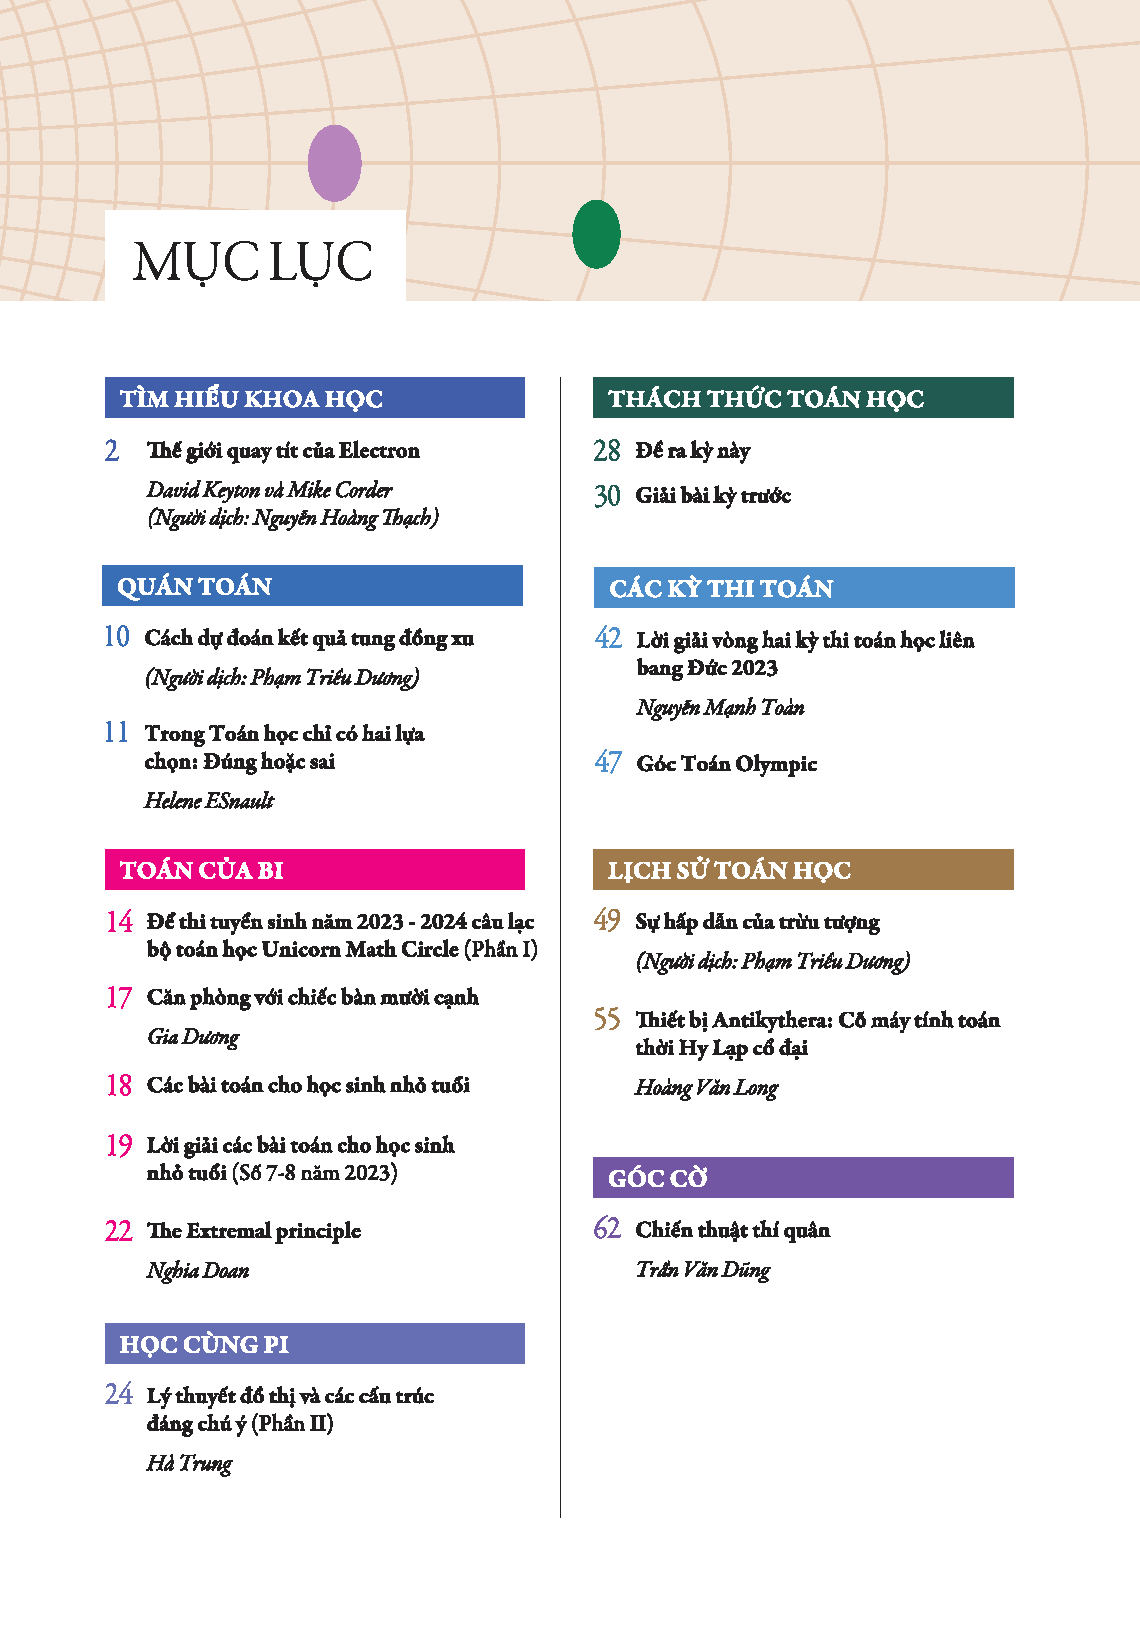
\includegraphics[scale=1]{ML.pdf}}}
%	 \centering
%	 \vspace*{0cm}
%	 \endgroup
%	 \newpage	  
%	 \pagestyle{empty}
%
%	\setcounter{page}{2}
%
%	\setcounter{figure}{0}
%	\thispagestyle{doisongtoanhocnone}
\pagestyle{doisongtoanhoc}
\everymath{\color{doisongtoanhoc}}
\graphicspath{{../doisongtoanhoc/pic/}}
%\blfootnote{$^1$\color{doisongtoanhoc}Viện Toán học.}
\begingroup
\AddToShipoutPicture*{\put(0,616){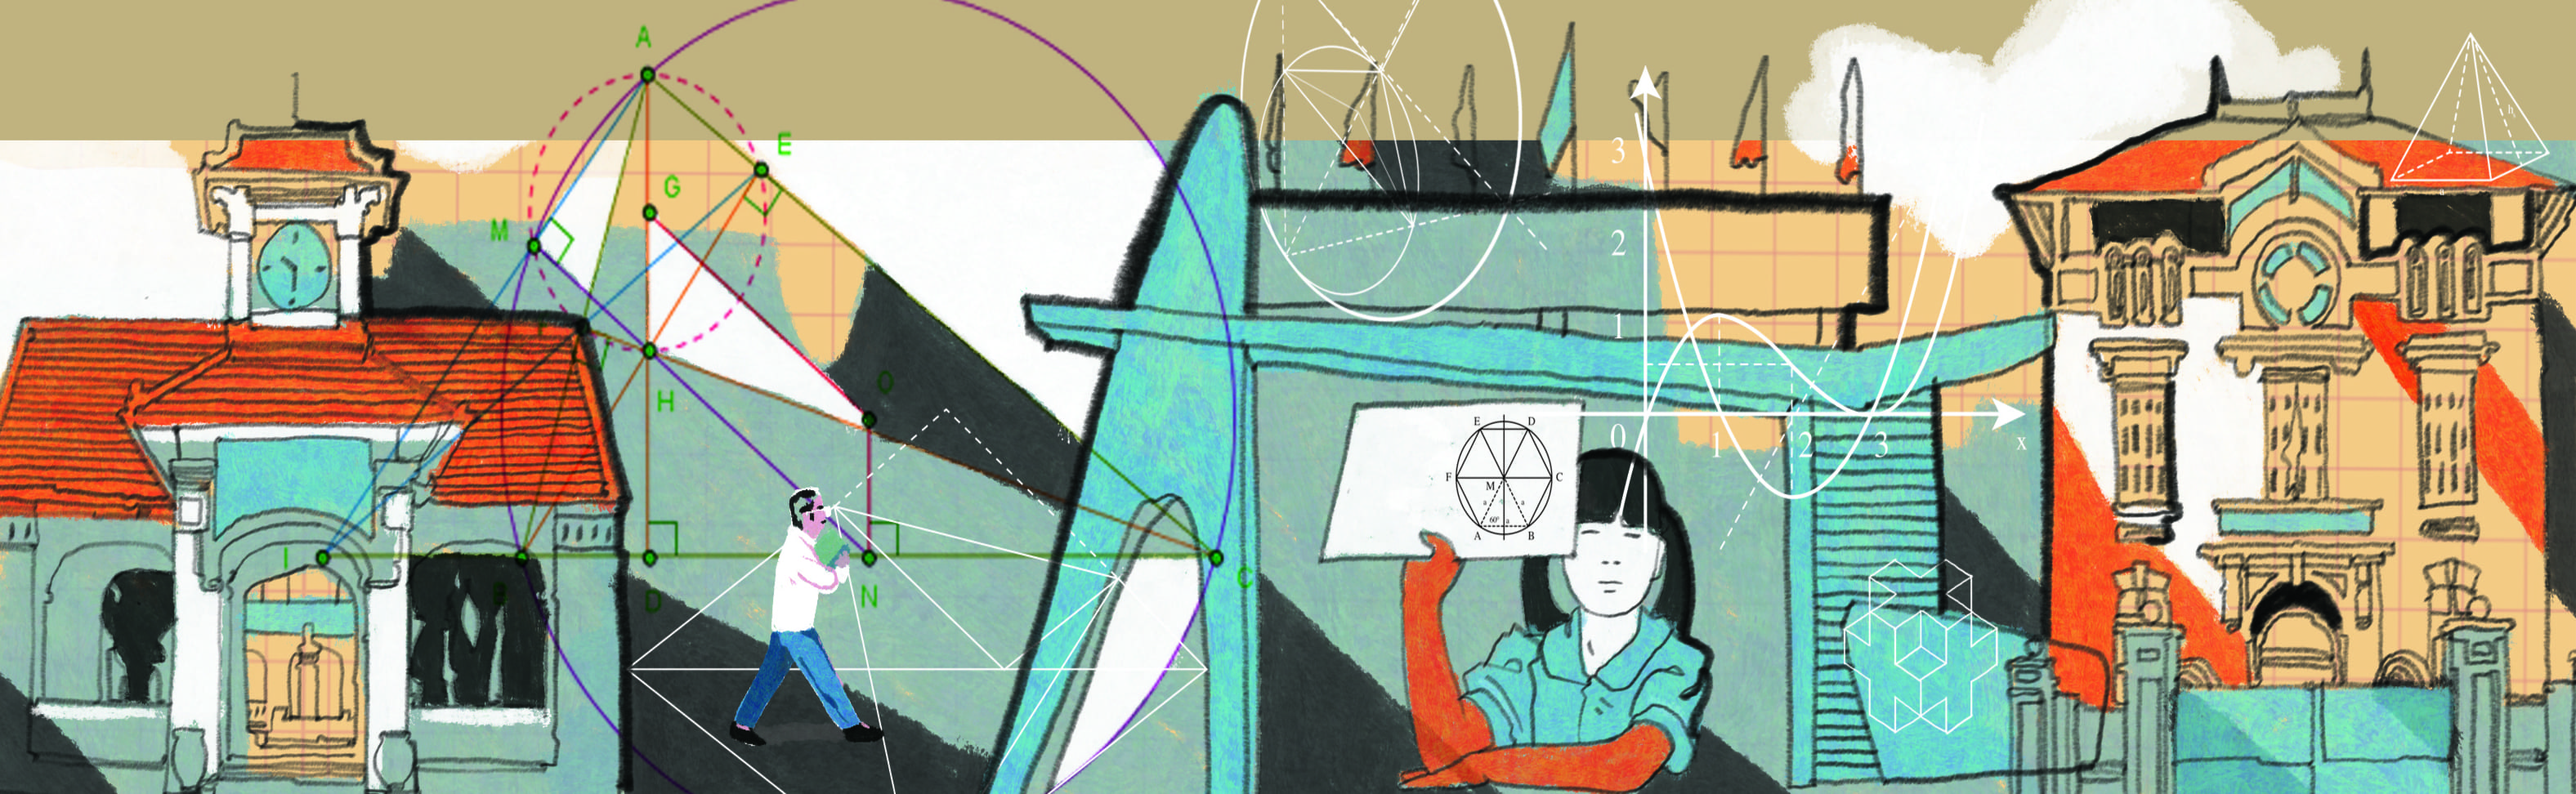
\includegraphics[width=19.3cm]{../bannerdoisong}}}
\AddToShipoutPicture*{\put(75,465){
\includegraphics[scale=1]{../tieude2.pdf}}}
\centering
\endgroup

\vspace*{245pt}

\begin{multicols}{2}
	\textbf{\color{doisongtoanhoc}I. Sơ lược tiểu sử}
	\vskip 0.1cm
	Giáo sư Hoàng Xuân Sính sinh ngày $5/9/1933$, là người gốc Làng Cót, Từ Liêm, Hà Nội. Khoảng những năm $40$, gia đình bà sinh sống tại $102$ Hàng Bông, và ngôi nhà của gia đình bà cũng chính là cơ sở xuất bản tờ báo Thanh Nghị, tiếng nói của trí thức yêu nước thời bấy giờ.
	\vskip 0.1cm
	Tốt nghiệp trường trung học Chu Văn An năm $1951$, bà được người cậu ruột đón sang học tiếp ở Pháp. Sau khi nhận bằng cử nhân toán học của Đại học Toulouse năm $1957$ và bằng thạc sỹ toán học năm $1959$, bà trở về nước đầu năm $1960$.
	\vskip 0.1cm
	``\textit{Tôi đã chọn con đường của nhiều trí thức yêu nước cùng thời, nhớ tới lời dạy của Bác Hồ đối với anh chị em Việt kiều: `Mỗi người cố học giỏi lấy một nghề, sau này trở về phục vụ Nhân dân'. Những lúc tổ quốc gian khó nhất, là những khi nhân dân cần chúng ta nhất. Tôi biết, trở về chính là yêu nước}".
	\vskip 0.1cm
	Năm $1975$ bà bảo vệ luận án tiến sỹ quốc gia\footnote[2]{\color{doisongtoanhoc}Tương đương với tiến sỹ
		khoa học ngày nay.} tại Paris, Pháp. Bản luận án ``Gr--Catégories" của bà là điểm khởi đầu của lý thuyết ``$n$--Catégories", một lý thuyết đang phát triển mạnh trên thế giới, có nhiều ứng dụng trong vật lý và khoa học tính toán. 
	\begin{figure}[H]
		\vspace*{-5pt}
		\centering
		\captionsetup{labelformat= empty, justification=centering}
		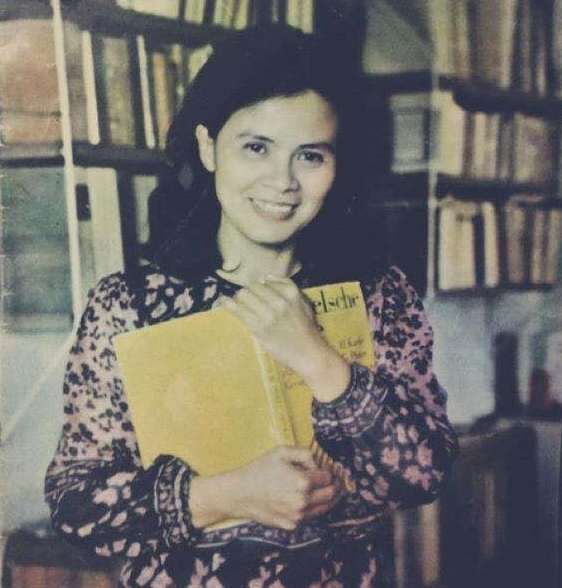
\includegraphics[width= 1\linewidth]{Anh1}
		%		\caption{\small\textit{\color{doisongtoanhoc}}}
		\vspace*{-15pt}
	\end{figure}
	Năm $1980$, bà được phong học hàm Giáo sư, và là nữ giáo sư toán học đầu tiên của Việt Nam.
	\vskip 0.1cm
	Năm $1998$, cùng với một số nhà toán học, bà thành lập Trung tâm Đại học Thăng Long, cơ sở giáo dục đại học ngoài công lập đầu tiên của Việt Nam, tiền thân của trường Đại học Thăng Long. 
	\vskip 0.1cm
	\textbf{\color{doisongtoanhoc}II. Bản luận án ``Gr-Catégories" }
	\vskip 0.1cm
	\textit{$1$. Gr--Categories.}
	\vskip 0.1cm
	Trong toán học, Hoàng Xuân Sính nổi tiếng với những kết quả trong lý thuyết phạm trù. Và cũng hơi có phần nghịch lý, khi hình như ở nước ngoài người ta biết rõ hơn cộng đồng toán học trong nước về những đóng góp của Hoàng Xuân Sính! Cũng có thể vì bà hầu như không nhắc đến những kết quả của mình.
	\vskip 0.1cm
	Phần này có mục tiêu giới thiệu sơ lược với những độc giả không là chuyên gia ngành toán về lý thuyết Gr--phạm trù và vị trí của nó trong toán học. Đây thực sự là nhiệm vụ rất khó khăn, bởi lẽ Gr--phạm trù là một lý thuyết rất sâu, không dễ tiếp cận ngay với những nhà toán học không trong chuyên ngành.  
	\vskip 0.1cm
	Trước tiên, xin đưa ra một định nghĩa không hình thức của \textit{phạm trù}.
	Khi mô tả bất kỳ một cấu trúc toán học nào, thậm chí bất kỳ một hiện tượng tự nhiên hay xã hội nào, ta đều cần chỉ ra hai điều mấu chốt: các \textit{đối tượng} được xét trong đó và \textit{quan hệ} giữa chúng.  
	\begin{figure}[H]
		\vspace*{-5pt}
		\centering
		\captionsetup{labelformat= empty, justification=centering}
		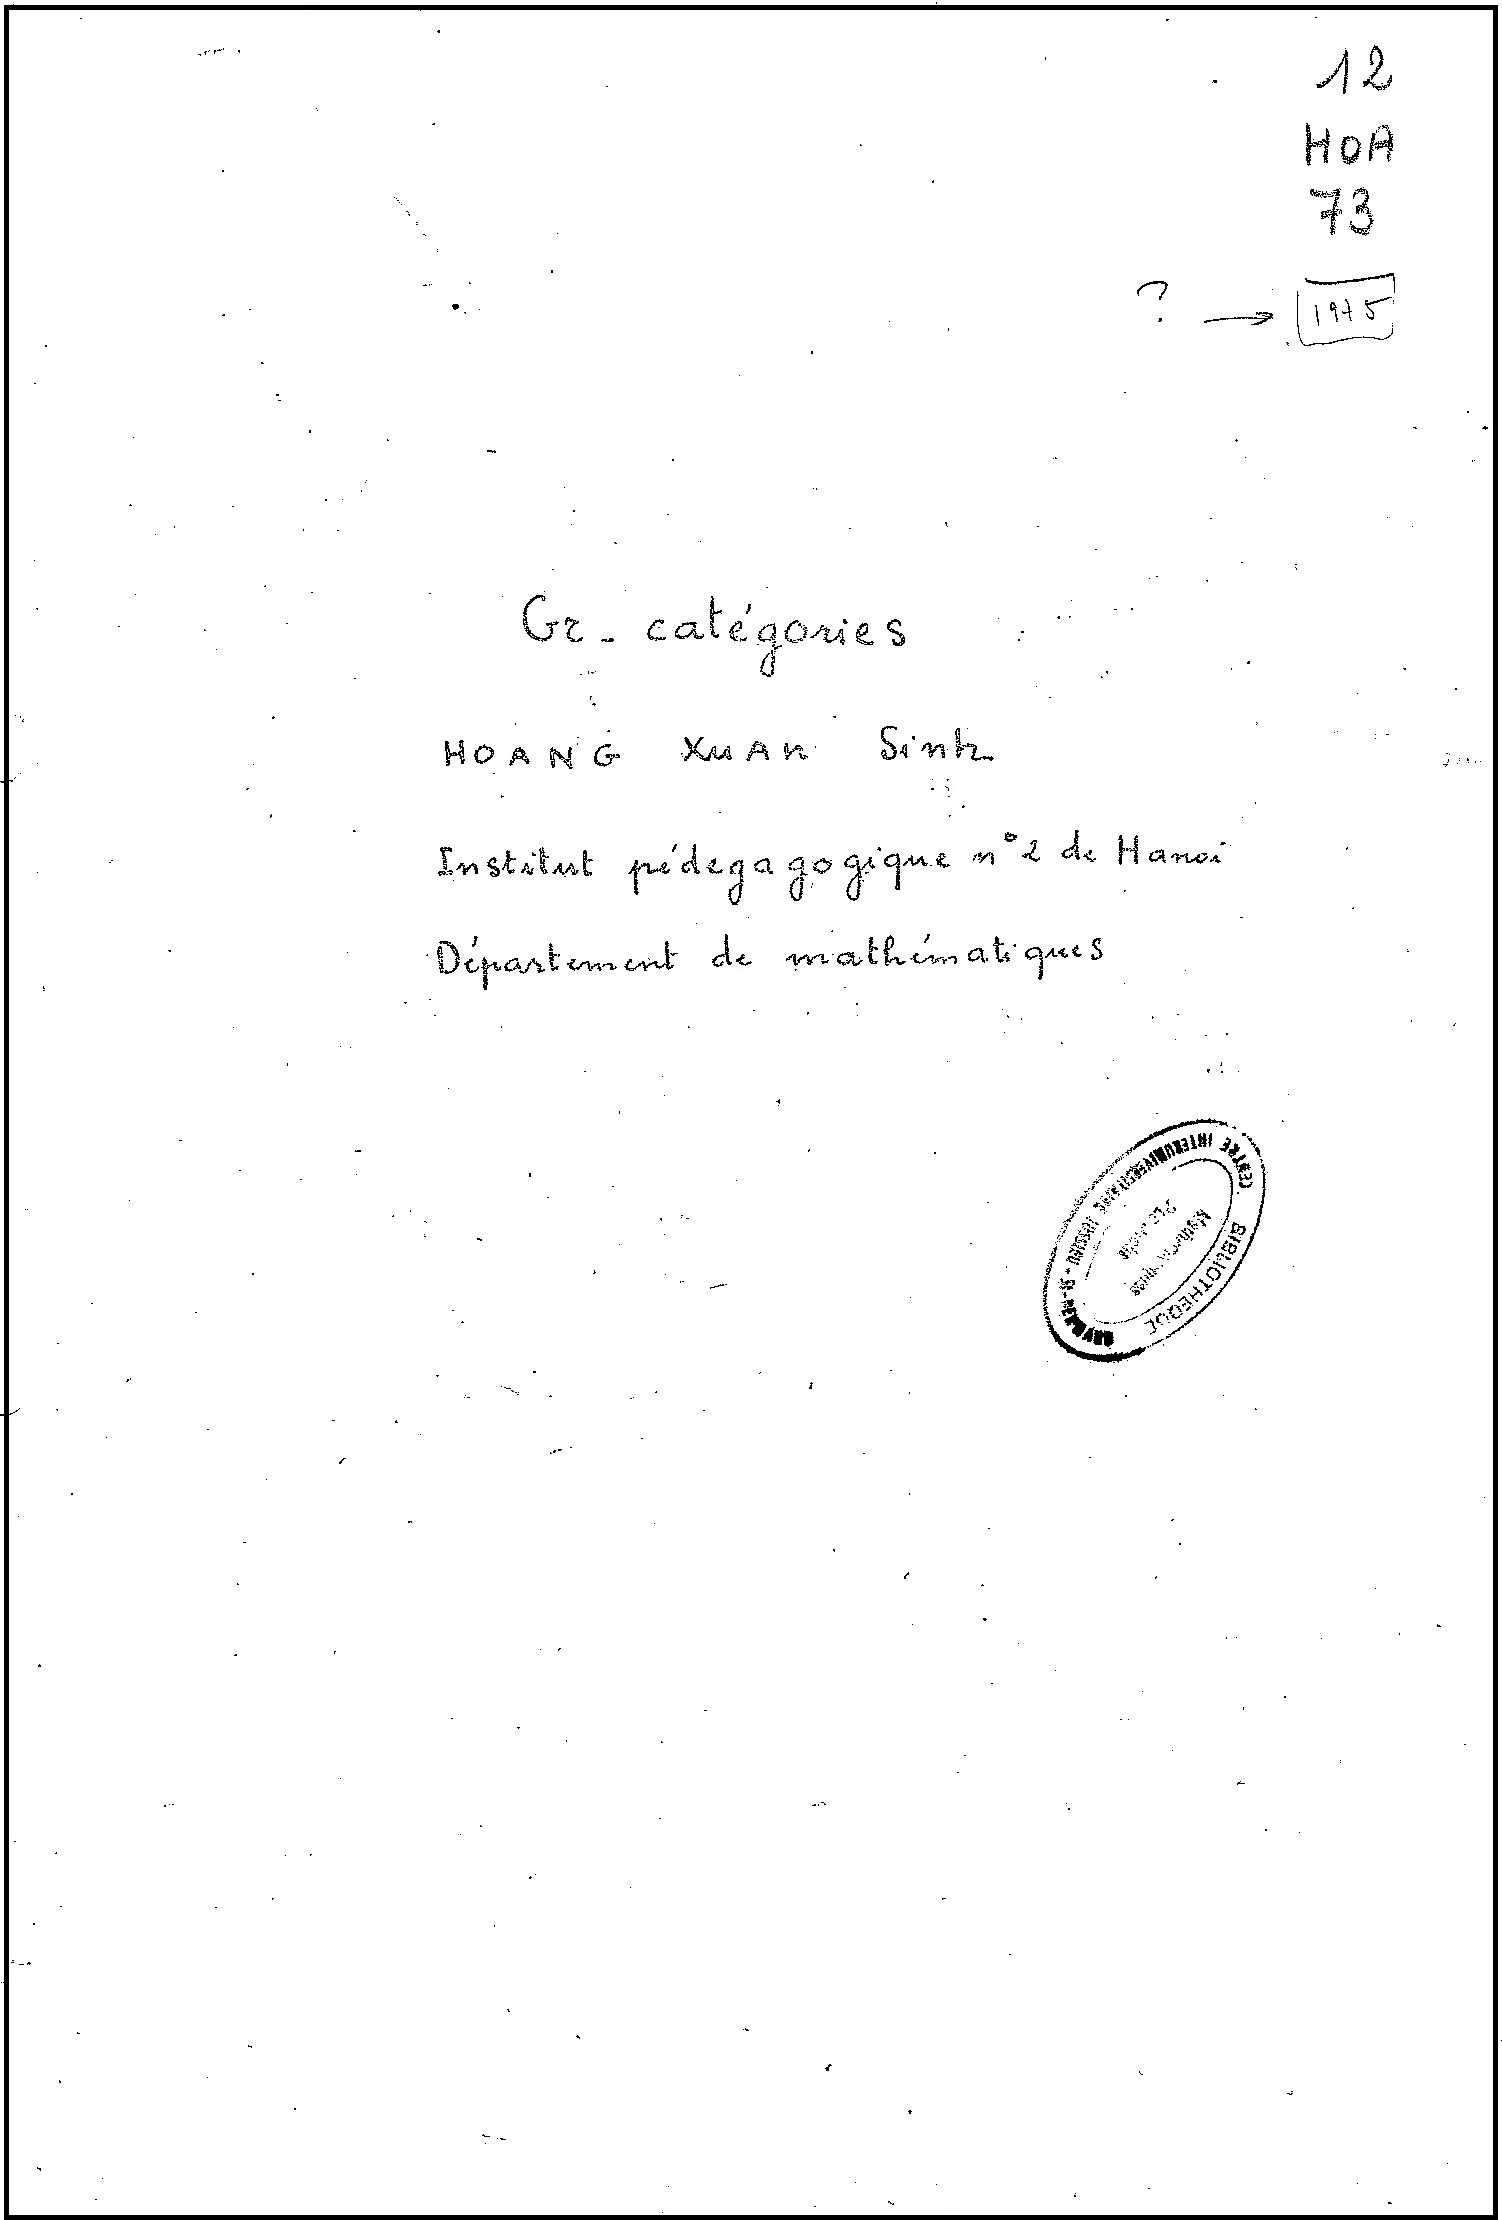
\includegraphics[height= 0.72\linewidth]{Anh21}
		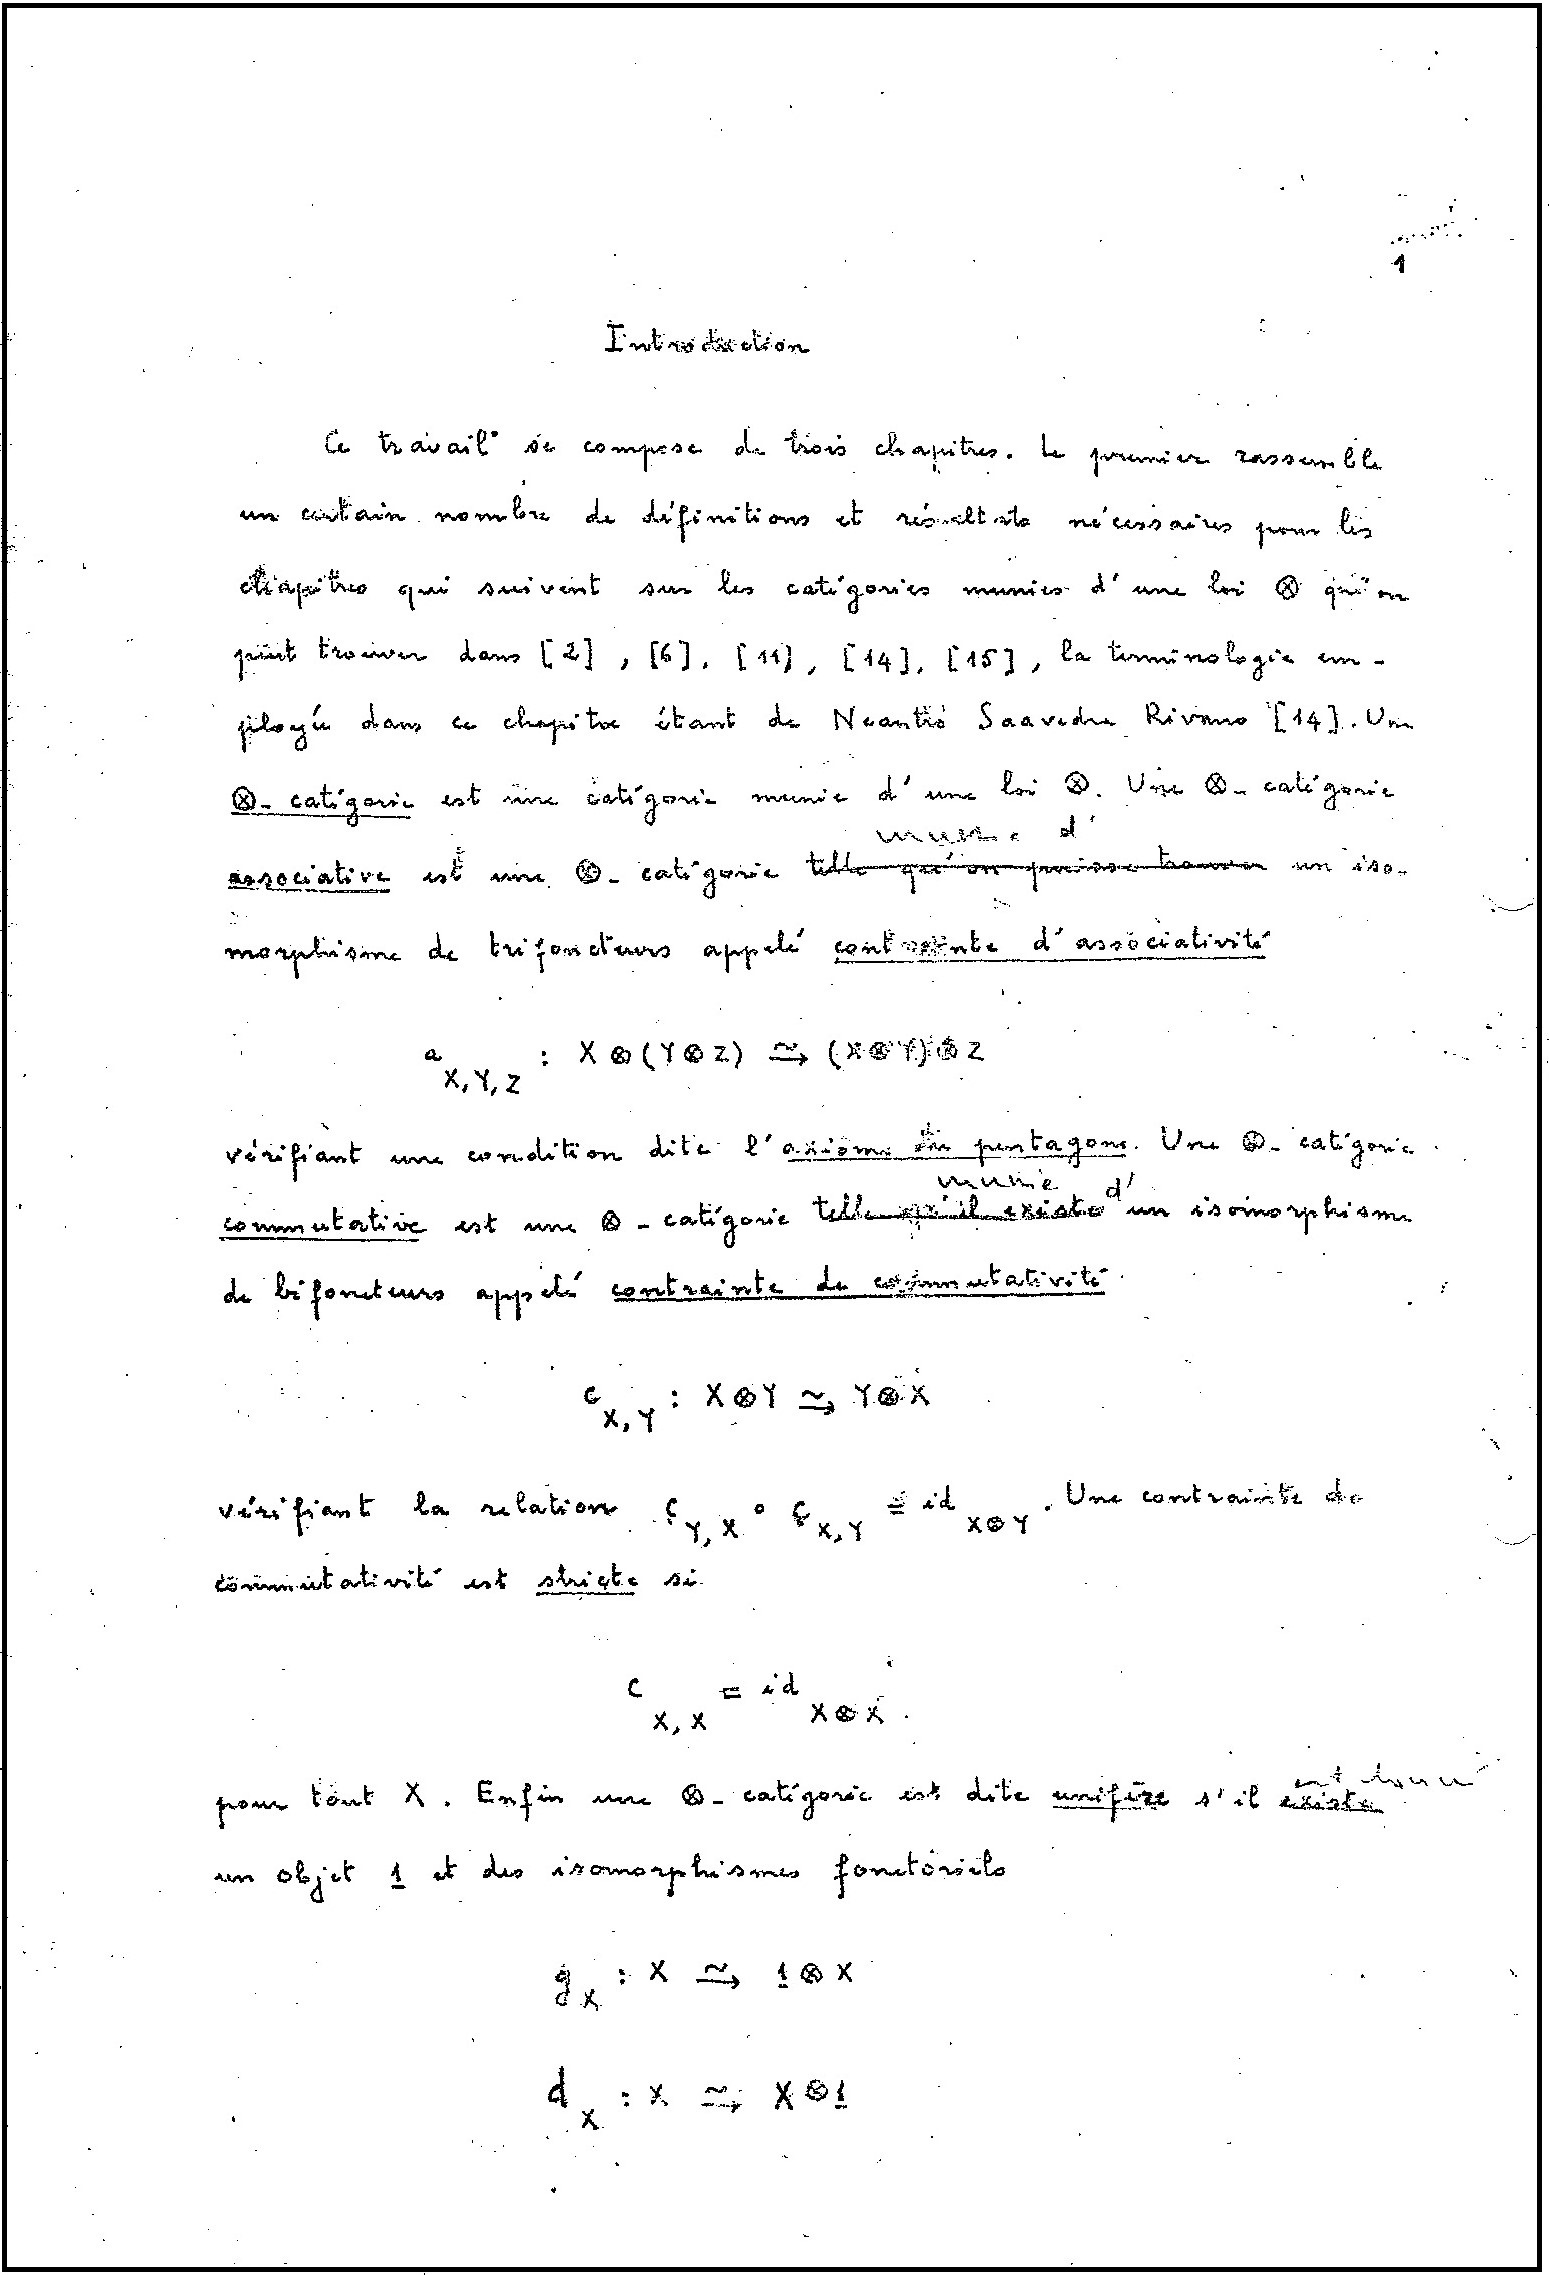
\includegraphics[height= 0.72\linewidth]{Anh22}
		%		\caption{\small\textit{\color{doisongtoanhoc}}}
		\vspace*{-10pt}
	\end{figure}
	Lý thuyết phạm trù ra đời nhằm cung cấp một ngôn ngữ tổng quát để nghiên cứu các cấu trúc toán học. Các đối tượng nghiên cứu ở đây được gọi là các ``vật", quan hệ giữa các vật được cho bởi những ``mũi tên" đi từ vật này đến vật khác. Nói đơn giản, phạm trù là một cặp gồm tập hợp các VẬT (objects), và tập hợp các MŨI TÊN giữa các  vật, gọi là các ``cấu xạ" (morphism).
	\vskip 0.1cm
	
	Có thể chỉ ra vài ví dụ:
	\vskip 0.1cm
	$1$/ \textit{Trong vật lý}: Tập hợp các \textit{trạng thái} của một  hệ vật lý nào đó lập thành tập hợp các ``vật". Quá trình \textit{chuyển trạng thái} cho ta ``cấu xạ" giữa các ``vật".
	\vskip 0.1cm
	$2$/ \textit{Trong tin học}: Các bộ \textit{dữ liệu} làm thành tập hợp các vật. \textit{Chương trình} là một cấu xạ chuyển bộ dữ liệu này thành bộ dữ liệu khác.
	\vskip 0.1cm
	$3$/ \textit{Trong logic}: Các \textit{mệnh đề} lập thành tập hợp các vật, \textit{chứng minh} là cấu xạ từ mệnh đề này đến mệnh đề khác.
	\vskip 0.1cm
	Như vậy, hầu hết cấu trúc trong toán học, và rộng hơn, trong tự nhiên và xã hội, có thể mô tả bằng ngôn ngữ phạm trù. Tuy nhiên, cũng chính vì phạm trù là cấu trúc quá tổng quát nên từ những kết quả của lý thuyết phạm trù, khó suy ra được những kết quả sâu sắc của các đối tượng thuộc những cấu trúc toán học khác. Vì thế, một yêu cầu tự nhiên là cần đưa vào cấu trúc phạm trù những phép toán nào đó để nó vẫn đủ tổng quát, nhưng có thể chứa đựng, và hơn nữa,  phát hiện những kết quả sâu sắc, chứ không chỉ đóng vai trò như một ngôn ngữ mô tả.
	\vskip 0.1cm
	Một trong những cấu trúc toán học quan trọng nhất là \textit{nhóm}. Khởi đầu từ công trình của Evariste Galois, lý thuyết nhóm đã trở thành công cụ không thể thiếu trong vật lý. Giáo sư Hoàng Xuân Sính đã đưa ra khái niệm \textit{Gr--phạm trù} và mô tả cấu trúc của chúng. Nói một cách ngắn gọn,  Gr--phạm trù là một phạm trù trong đó trang bị phép tính với ràng buộc kết hợp, đồng thời các vật và các cấu xạ đều có tính chất khả nghịch. Do đó, Gr--phạm trù ``giống như" một nhóm (chữ ``Gr" xuất phát từ ``group", là \textit{nhóm}).
	\vskip 0.1cm
	$2$. \textit{Sinh's Invariant.}
	\vskip 0.1cm
	Một bài toán lớn trong toán học, cũng như trong những ngành khoa học khác, là bài toán phân loại. Để xác định một đối tượng có những tính chất cơ bản gì, chúng ta cần biết chúng thuộc loại nào. Điều này chỉ làm được nếu tìm ra thuộc tính của các đối tượng cùng một  loại, tức là tìm ``bất biến" của lớp đối tượng đó. Nếu một đối tượng mang ``bất biến" của lớp nào, ta biết nó thuộc lớp đó,  tương tự như vân tay là ``bất biến" để nhận biết mỗi người.
	\vskip 0.1cm
	Trong luận án của mình, giáo sư Hoàng Xuân Sính đã tìm ra một bất biết để nhận biết một lớp các không gian ``đủ tốt", gọi là các \textit{CM--complex}. Cụ thể hơn, khi cho một Gr--phạm trù, ta được hai nhóm: nhóm $G$ các lớp đẳng cấu của các vật, và nhóm $A$ các tự đẳng cấu của vật đơn vị (cũng vì thế, ngày nay người ta gọi Gr--phạm trù là $2$--\textit{nhóm}, và phát triển lý thuyết này thành lý thuyết các \textit{$n$--nhóm}). Một Gr--phạm trù có thể đặc trưng hoàn toàn bởi lớp [$a$] trong nhóm đối đồng điều $H^3(G, A)$. Lớp này ngày nay được mang tên là \textit{bất biến Sính} (Sinh's invariant).
	\vskip 0.1cm
	Theo John Baez, một nhà toán học nổi tiếng, ``\textit{kết quả của Hoàng Xuân Sính rọi ánh sáng lên vấn đề nghiên cứu kiểu đồng luân của các không gian tương đối `đẹp', chẳng hạn các CW--complex}"\footnote[3]{\color{doisongtoanhoc}John Baez, Hoang Xuan Sinh's thesis: categorifying Group Theory, Thang Long Journal of Mathematics and Mathematical Sciences, Vol.3, N–1, 2023.}.   
	\vskip 0.1cm
	Hướng nghiên cứu mà giáo sư Hoàng Xuân Sính khởi đầu từ những năm $1967-1975$ ngày nay đang phát triển mạnh, gọi là $n$--\textit{phạm trù} ($n$--\textit{Category}). Gần đây, những kết quả trong lý thuyết $n$--category được sử dụng trong tính toán lượng tử, cơ sở lý thuyết của các máy tính lượng tử trong tương lai.
	\vskip 0.1cm
	Lý thuyết Gr--phạm trù được xây dựng trong bản luận án \textit{Gr--Catégories} của Giáo sư Hoàng Xuân Sính, một bản luận án có số phận đặc biệt trong lịch sử toán học. 
	\vskip 0.1cm
	Trong đợt làm việc tại Việt Nam cuối năm $1967$, A. Grothendieck -- một trong những nhà toán học vĩ đại nhất thế kỷ XX -- gợi ý giáo sư Hoàng Xuân Sính nghiên cứu xây dựng một kiểu phạm trù sao cho nó gần như một nhóm. Ý tưởng của Grothendieck được thực hiện thành công, và Gr--phạm trù ra đời. Thực ra, ý đồ của Grothendieck xa hơn nhiều: trong tài liệu dày $600$ trang (\textit{Pursuing Stacks}, $1984$. arXiv:$2111.010000$) Grothendieck đưa ra \textit{giả thuyết đồng luân} như sau: ``\textit{Một CW--complex $X$ gọi là kiểu $n$ nếu nhóm $\pi_k(X)$ là tầm thường với $k > n$. Có thể phân lớp sai khác tương đương đồng luân các CW kiểu $n$ bởi các cấu trúc gọi là $n$--nhóm}". Cho đến nay, mới có hai trường hợp được thực hiện hoàn chỉnh là $n =1$ với phạm trù monoidal của Eilenberg -- Mac Lane và  $n = 2$ trong luận án của giáo sư Hoàng Xuân Sính. Trường hợp $n > 2$ vẫn đang được quan tâm nghiên cứu và mới có những kết quả riêng rẽ.
	\begin{figure}[H]
		\vspace*{-5pt}
		\centering
		\captionsetup{labelformat= empty, justification=centering}
		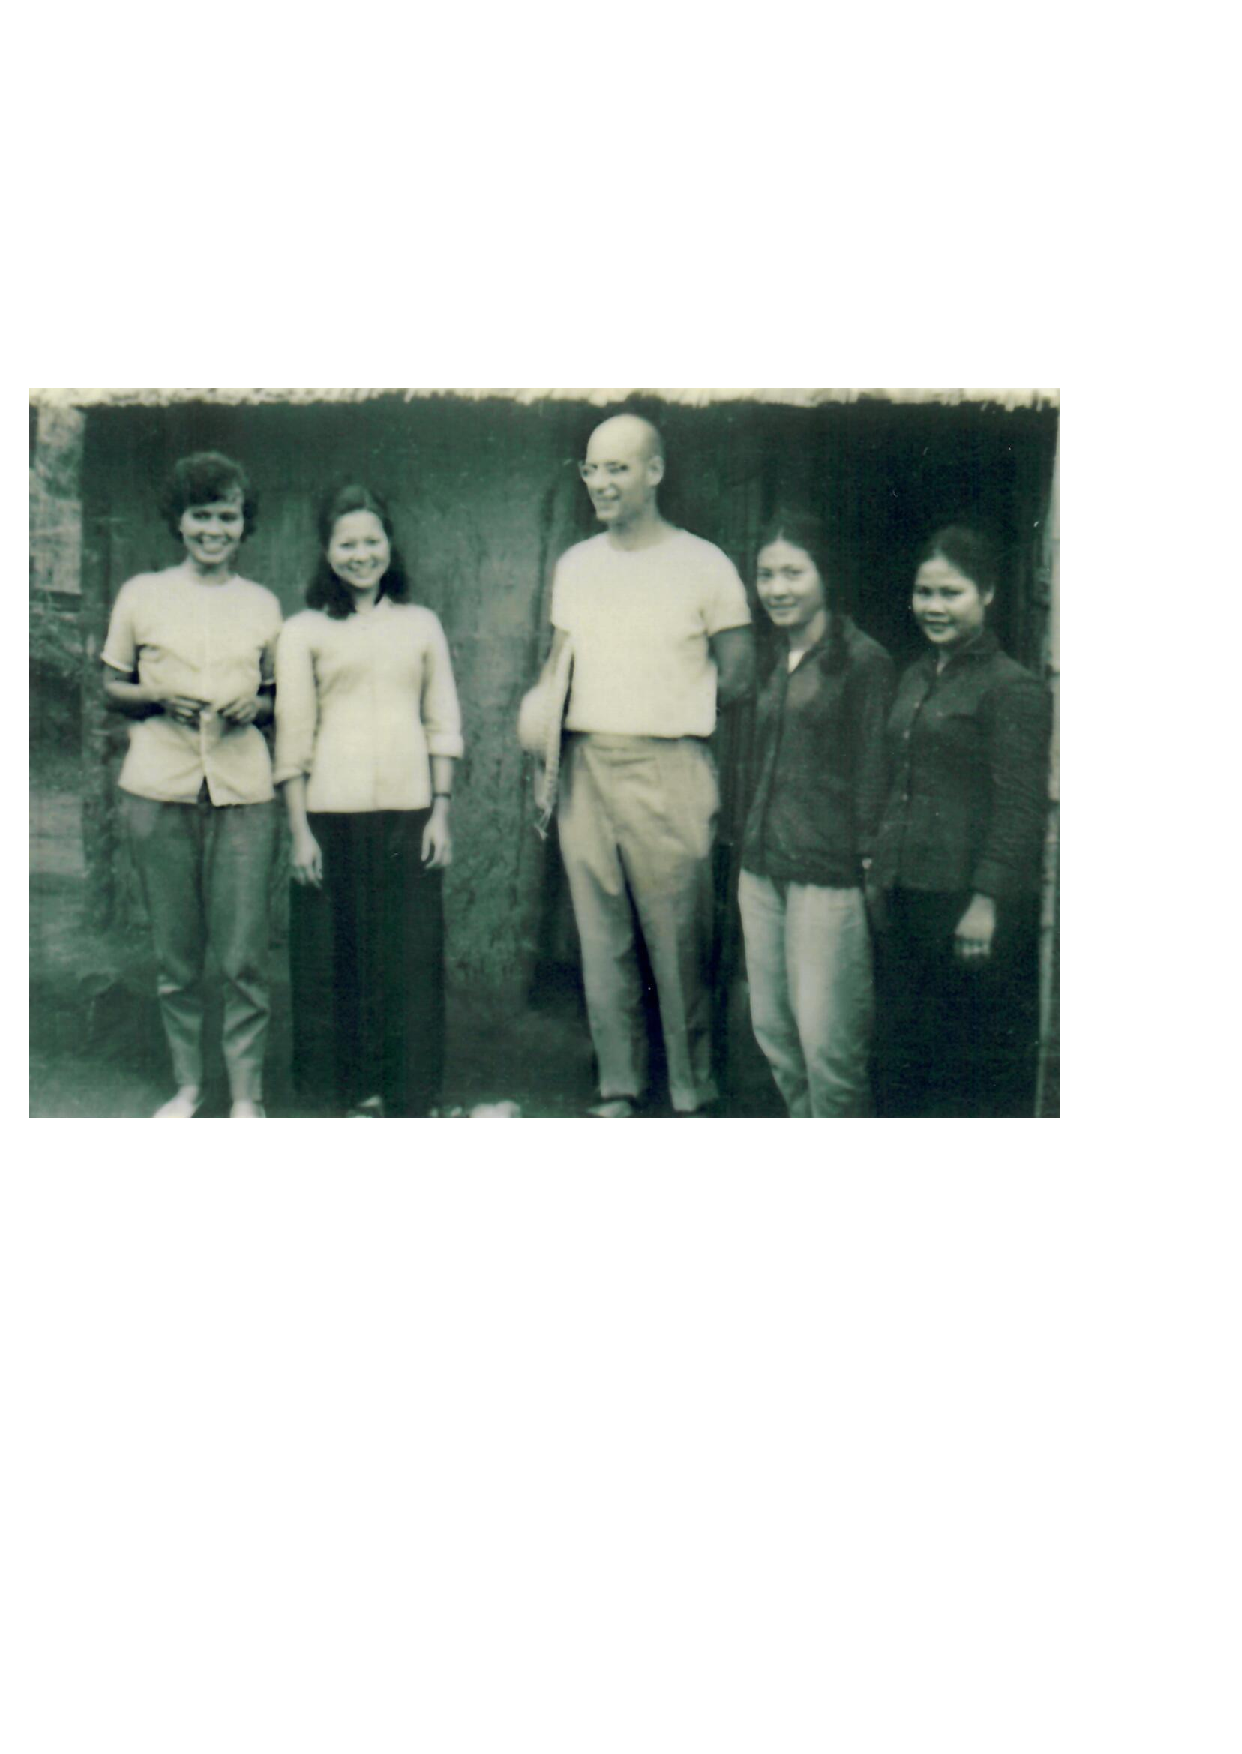
\includegraphics[width= 1\linewidth]{Anh3}
%		\caption{\small\textit{\color{doisongtoanhoc}}}
		\vspace*{-10pt}
	\end{figure}
	Trong suốt thời gian làm luận án, giáo sư Hoàng Xuân Sính chỉ liên hệ với Grothendieck $3$ lần, qua những bức thư ngắn chỉ đến được với người nhận sau hơn nửa năm! Thật khó tìm được luận án tiến sỹ nào khác trên thế giới được viết trong chiến tranh, trong điều kiện hoàn toàn cô lập với thế giới toán học, không có nhóm nghiên cứu, thiếu tài liệu, và thậm chí thiếu cả những điều kiện tối thiểu như giấy bút, ánh sáng và những bữa ăn no! Giáo sư Hoàng Xuân Sính kể rằng, khi ở khu sơ tán, ước mơ của bà nhiều khi chỉ là làm sao có đủ pin để ngồi làm việc trong màn, tránh được đàn muỗi dày đặc quanh chiếc đèn dầu!
	\vskip 0.1cm
	Bản luận án \textit{Gr--Catégories} làm thế giới toán học quan tâm và ngạc nhiên, không chỉ vì nội dung, mà còn ở sự ra đời đặc biệt của nó. 
	\vskip 0.1cm
	Luận án được hoàn thành năm $1973$, và bản \textit{viết tay} của nó được gửi cho Grothendieck. Sau nhiều trắc trở, năm $1975$ Hoàng Xuân Sính được phép ghé Paris trên đường trở về từ Đại hội Toán học Thế giới ở Vancouver để bảo vệ luận án tiến sỹ quốc gia. Hội đồng chấm luận án của bà cũng thật hiếm thấy, khi gồm những nhà toán học nổi tiếng nhất: H. Cartan, A. Grothendieck,  J. L. Verdier, L. Schwartz, M. Zisman.
	\vskip 0.1cm
	Những tháng gần đây, nhân sinh nhật lần thứ $90$ của giáo sư Hoàng Xuân Sính,   trên báo chí có nhiều có nhiều bài viết về ``sự trở về kỳ diệu" của bản luận án viết tay \textit{Gr--Catégories}. Tuy nhiên, với những nhà toán học thì sự trở về kỳ diệu chỉ thực sự xẩy ra khi những kết quả của họ được nhắc đến, được tiếp tục phát triển sau hơn nửa thế kỷ! Bản luận án của giáo sư Hoàng Xuân Sính đã trở về, và ở lại mãi mãi với toán học, trong những nghiên cứu về \textit{Sinh's invariant và $n$--phạm trù.}
	\vskip 0.1cm
	Xin dẫn vài lời đánh giá của  J. Baez:
	\vskip 0.1cm
	``\textit{Sẽ là thiếu sót nếu không đề cập đến việc các Gr--phạm trù,  ngày nay thường được gọi là $2$--nhóm,  đã có một sức sống mới trong vật lý lý thuyết và toán học.
	\vskip 0.1cm
	Lý do là vì} Lý thuyết trường chuẩn (Gauge Theory), \textit{cách tiếp cận thành công ngoạn mục của vật lý dựa trên các nhóm, có thể được khái quát hóa thành lý thuyết trường chuẩn bậc cao bằng cách sử dụng $2$--nhóm.
	\vskip 0.1cm
	Hơn nữa, không có lý do gì để dừng lại ở $2$ nhóm ... Có những hy vọng rằng một ngày nào đó các nhà vật lý sẽ tổng hợp các pha của vật chất được mô tả bởi lý thuyết trường chuẩn bậc cao. Đó sẽ là sự hiện thực hóa tuyệt vời tầm nhìn của Hoàng Xuân Sính.}"
	\vskip 0.1cm
	Những năm sau này, giáo sư Hoàng Xuân Sính không còn thời gian dành cho nghiên cứu toán học, khi dồn hết sức lực và tâm huyết để xây dựng trường Đại học Thăng Long. 
	\begin{figure}[H]
		\vspace*{-5pt}
		\centering
		\captionsetup{labelformat= empty, justification=centering}
		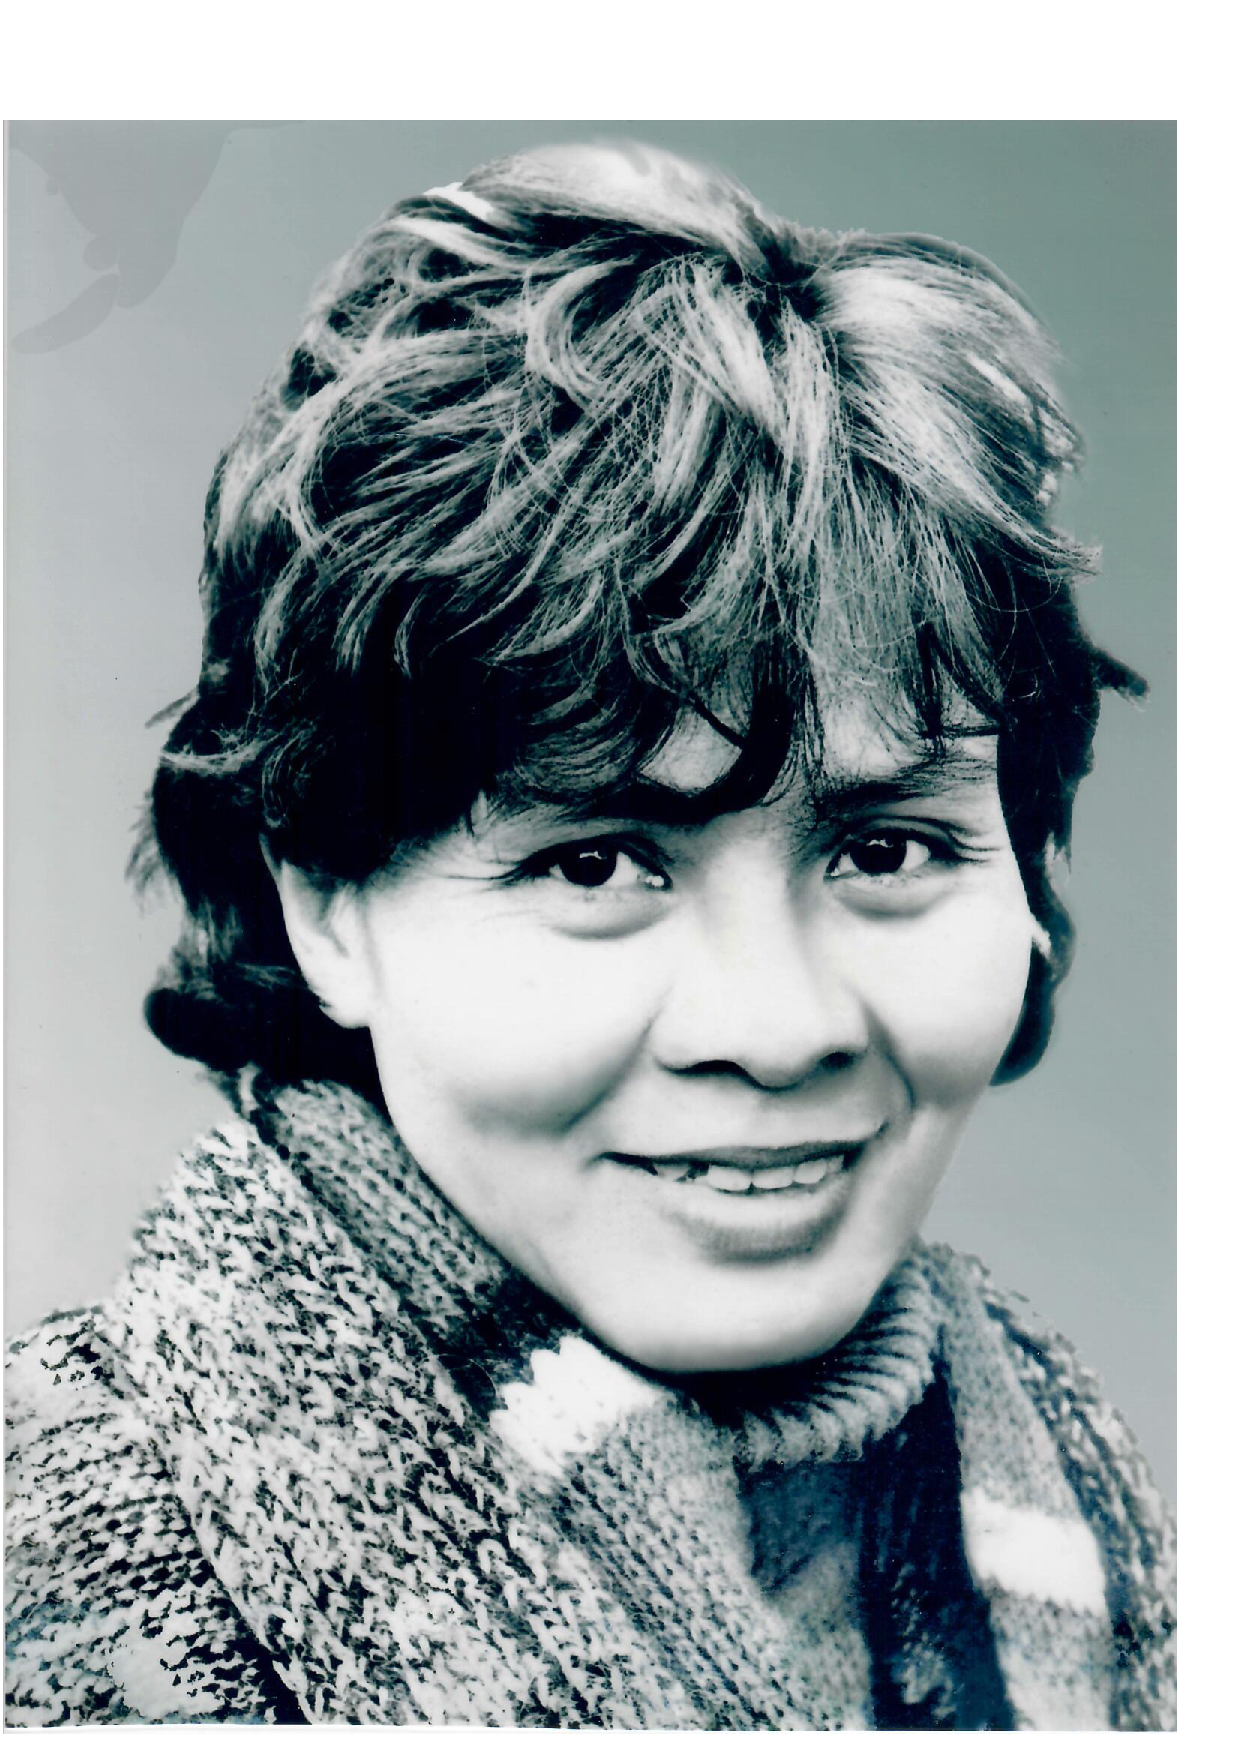
\includegraphics[width= 1\linewidth]{Anh12}
		\caption{\small\textit{\color{doisongtoanhoc}}}
		\vspace*{-20pt}
	\end{figure} 
	Cuộc đời bà là hành trình nhất quán của một trí thức yêu nước và nhà khoa học đầy tài năng: từ quyết định rời bỏ cuộc sống tiện nghi ở nước Pháp để trở về đóng góp cho nền giáo dục Việt Nam trong những năm chiến tranh ác liệt, quyết tâm vươn lên đỉnh cao khoa học trong những điều kiện đặc biệt khó khăn, cho đến những cố gắng và nghị lực phi thường để vượt qua biết bao thử thách, xây dựng trường đại học ngoài công lập đầu tiên trong hệ thống giáo dục của Việt Nam.
	\vskip 0.1cm
	Nếu như trong toán học, ``bất biến Sính" là một lớp đối đồng điều, thì ``bất biến Sính" trong cuộc đời chính là tình yêu của bà với tổ quốc và khoa học. 
\end{multicols}
%	\newpage
%
%	\thispagestyle{empty}


%	\begingroup 
%	\AddToShipoutPicture*{\put(0,0){\includegraphics[width=19.5cm]{MV.pdf}}}
%	\centering
%	\vspace*{0cm}
%	\endgroup
%	\newpage	
%	\pagestyle{empty}
%
%	\thispagestyle{empty}
%	\begingroup 
%	\AddToShipoutPicture*{\put(0,0){\includegraphics[width=19.45cm]{QC}}}
%	\centering
%	\vspace*{0cm}
%	\endgroup
%	\newpage	 
%	\pagestyle{empty}
%
	\setcounter{figure}{0}
	\thispagestyle{toancuabinone}
\pagestyle{toancuabi}
\everymath{\color{toancuabi}}
\blfootnote{$^1$\color{toancuabi}Trường Liên cấp Hội nhập Quốc tế iSchool Quảng Trị.}
\graphicspath{{../toancuabi/mecung/}}
\begingroup
\AddToShipoutPicture*{\put(0,616){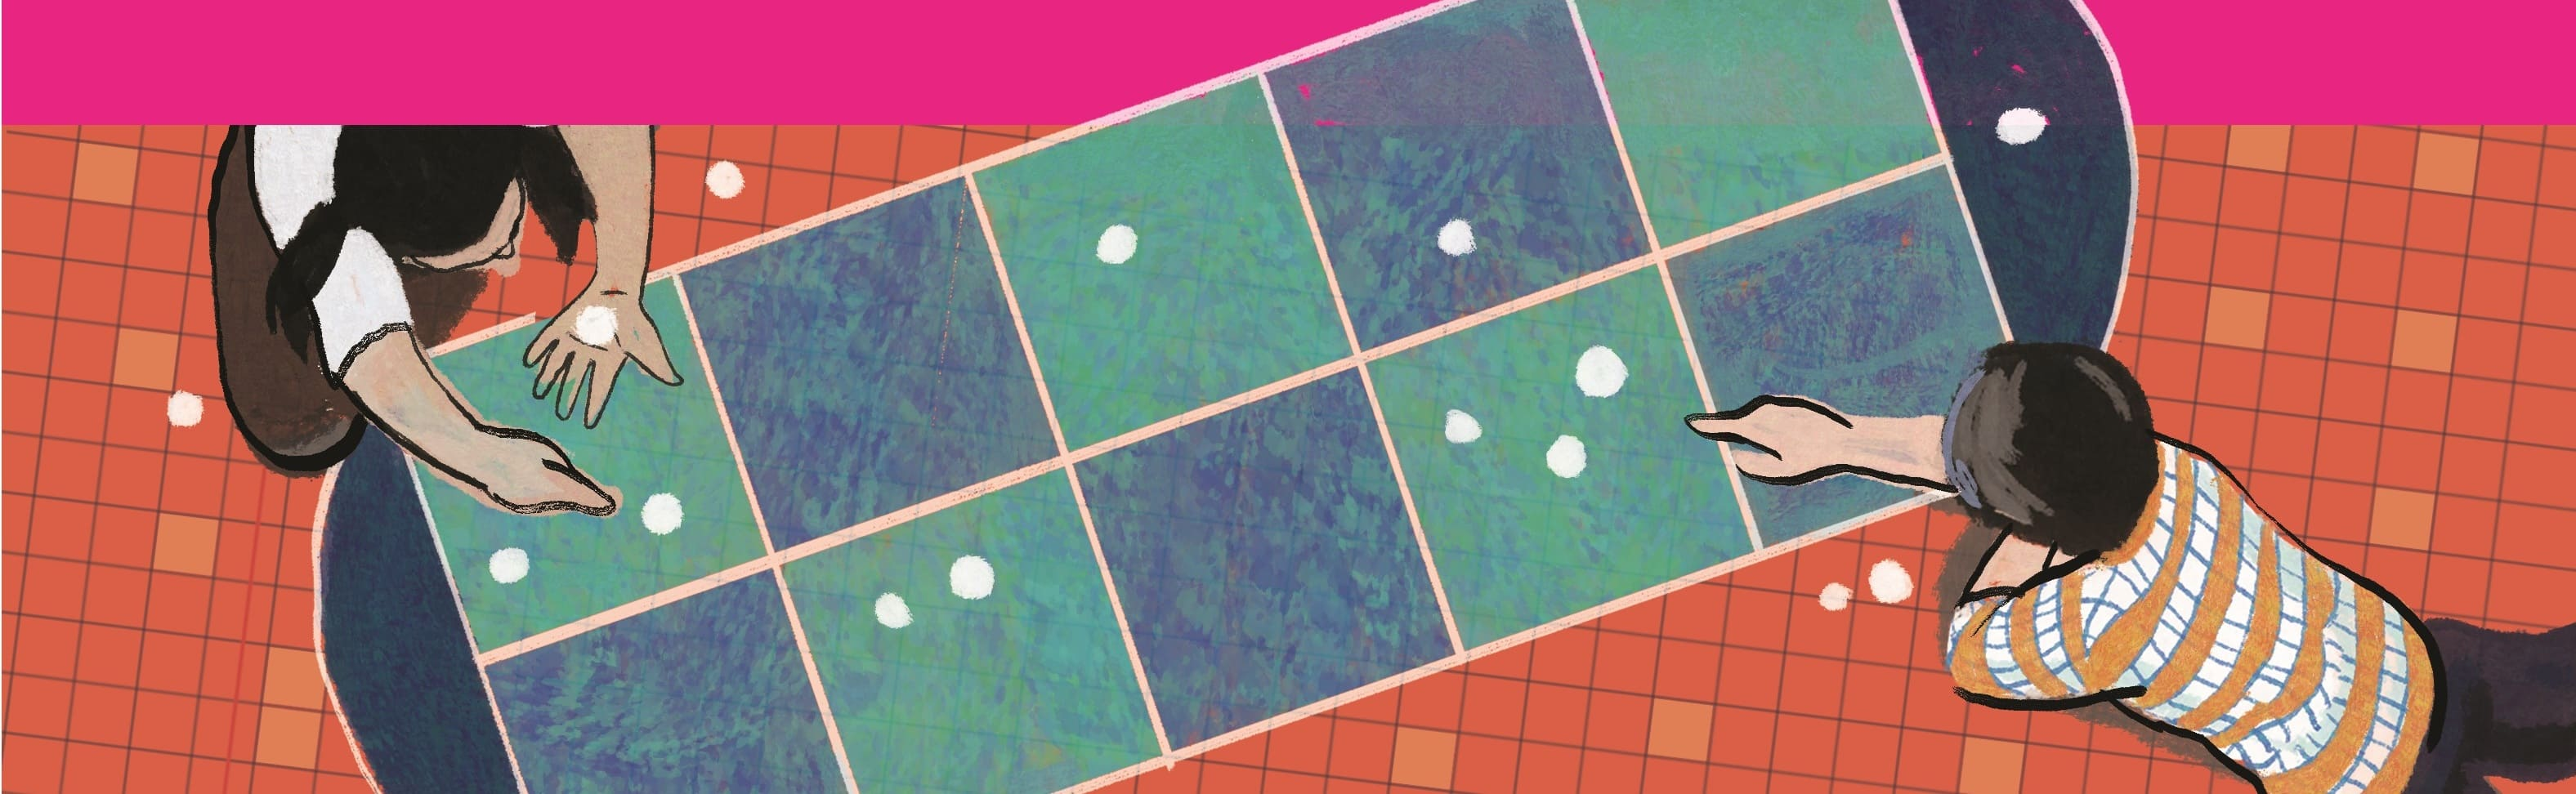
\includegraphics[width=19.3cm]{../bannertoancuabi}}}  
\AddToShipoutPicture*{\put(68,525){
\includegraphics[scale=1]{../tieudehihi2.pdf}}}  
\centering
\endgroup
\vspace*{185pt} 

\definecolor{bulgarianrose}{rgb}{0.28, 0.02, 0.03}
\begin{multicols}{2}
	$\pmb{2.}$ \textbf{\color{toancuabi}Làm trò chơi mê cung từ bìa giấy}
	\vskip 0.1cm
	\textbf{\color{toancuabi}Bước $\pmb{1}$:} Cắt các miếng bìa giấy hình chữ nhật với kích thước như hình bên dưới (đơn vị: cm).
	\begin{figure}[H]
		\vspace*{-5pt}
		\centering
		\captionsetup{labelformat= empty, justification=centering}
		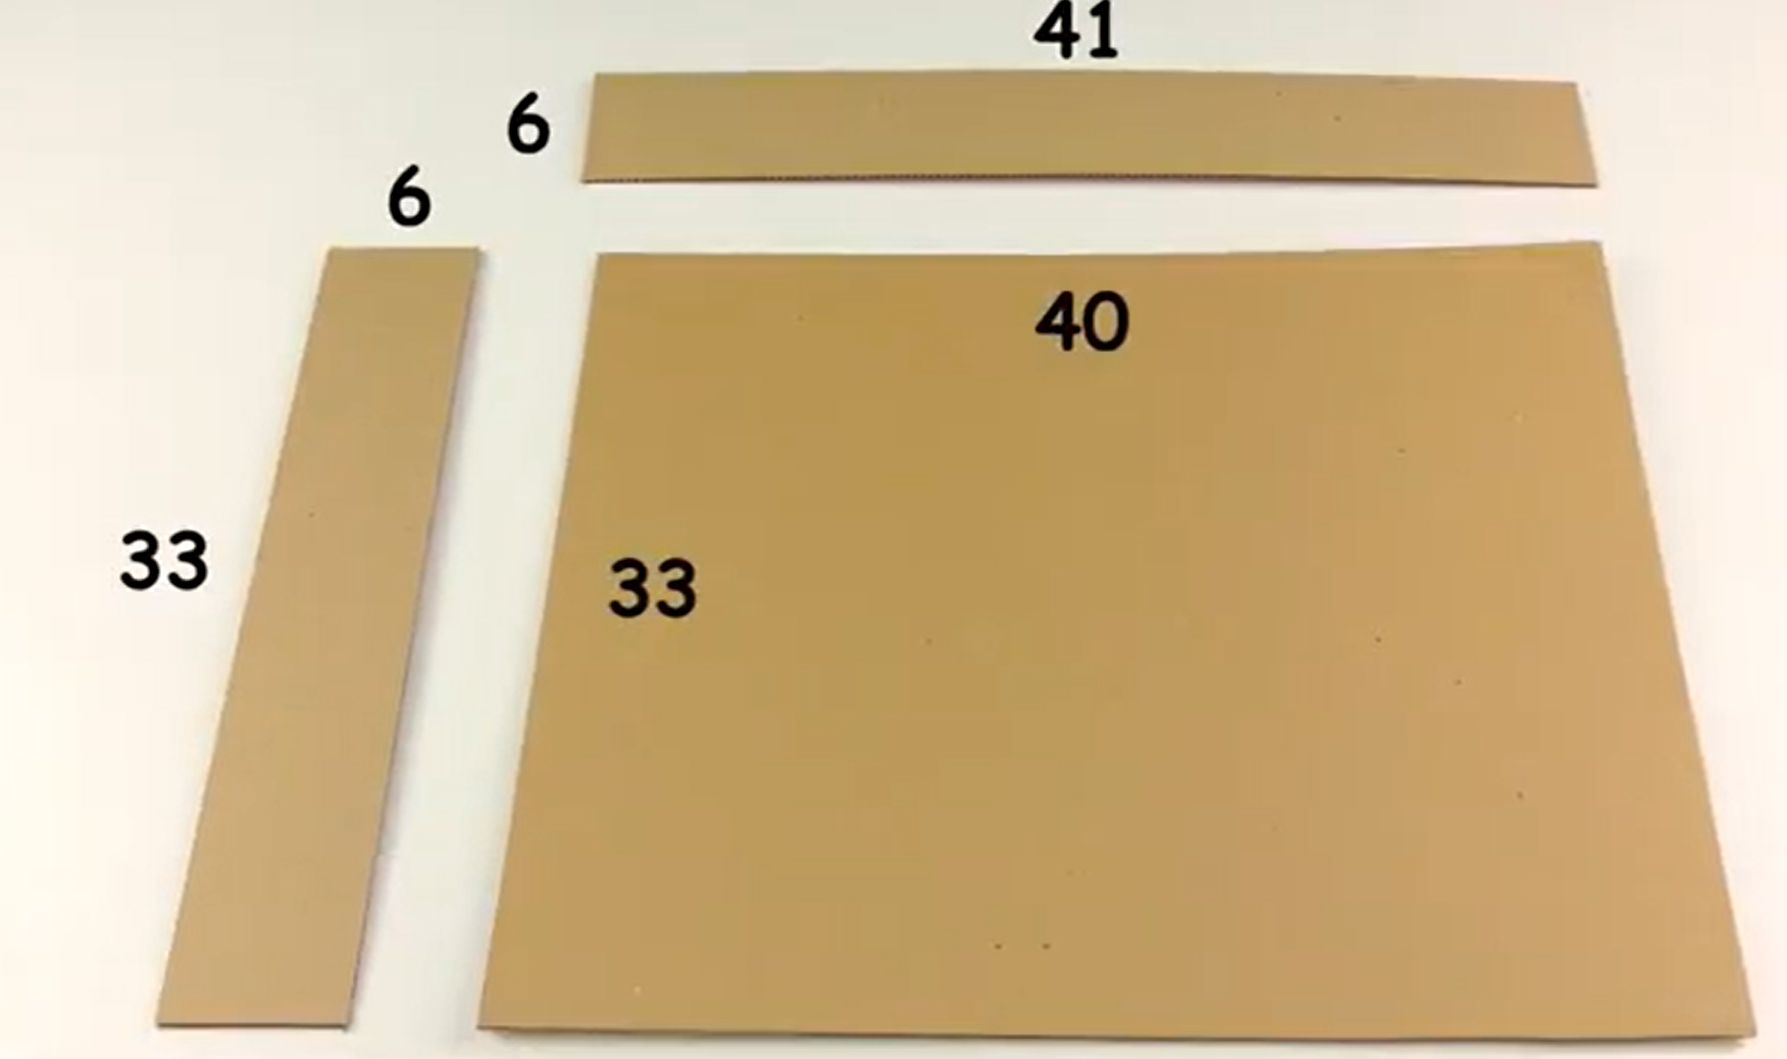
\includegraphics[width= 0.85\linewidth]{1}
%		\caption{\small\textit{\color{}}}
		\vspace*{-10pt}
	\end{figure}
	\textbf{\color{toancuabi}Bước $\pmb{2}$:} Sử dụng hồ dán để dán hai miếng bìa giấy lớn nhất với nhau nhằm tăng độ dày của miếng bìa giấy.
	\begin{figure}[H]
		\vspace*{-5pt}
		\centering
		\captionsetup{labelformat= empty, justification=centering}
		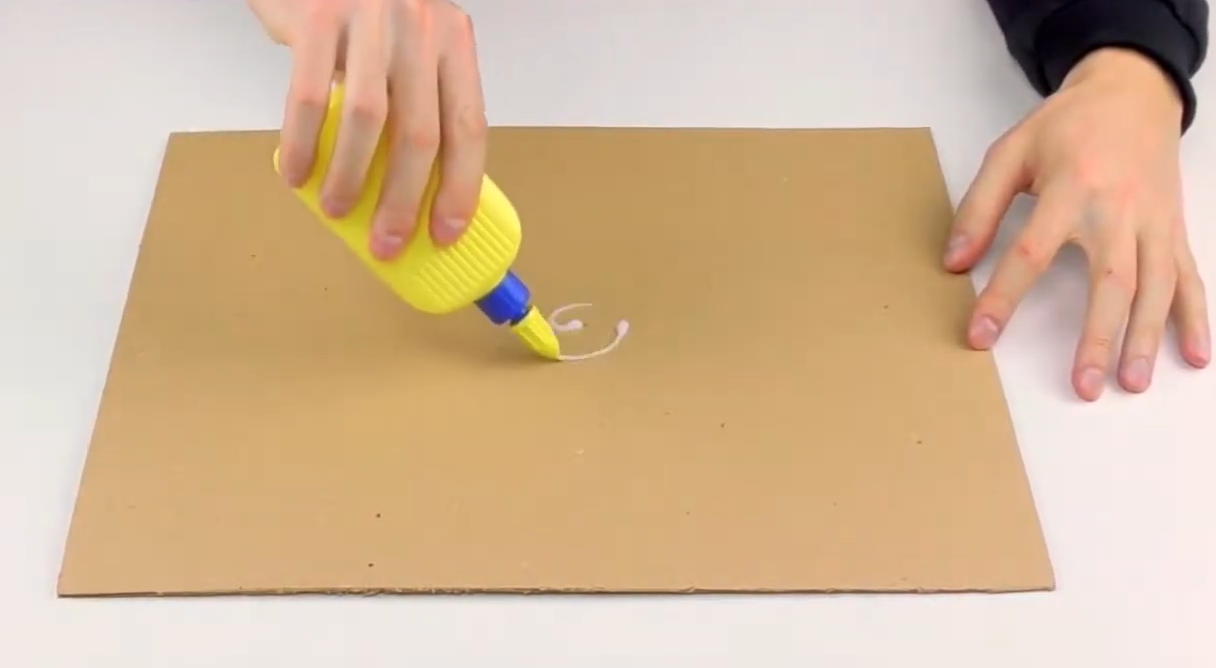
\includegraphics[width=0.85\linewidth]{2}
		
		\vspace*{1pt}
		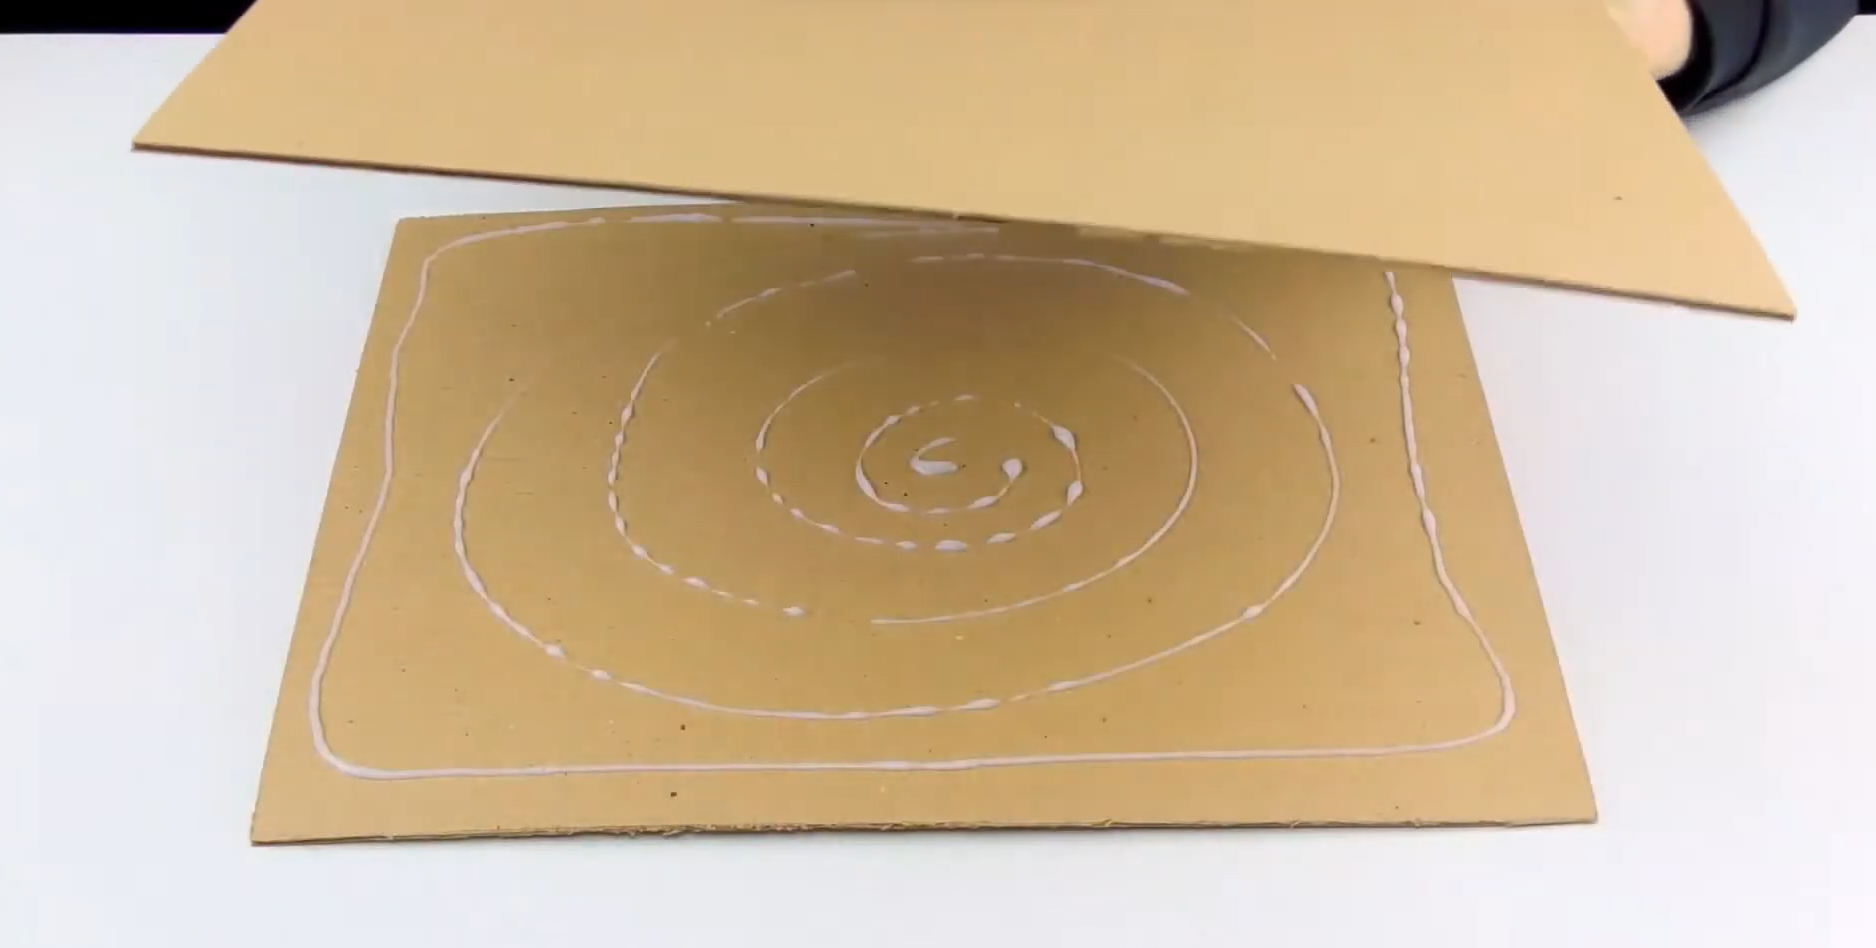
\includegraphics[width=0.85\linewidth]{3}
		\vspace*{-5pt}
	\end{figure}
	\textbf{\color{toancuabi}Bước $\pmb{3}$:} Tương tự, các em hãy làm tăng độ dày của cả $4$ miếng bìa giấy nhỏ nhé!
	\begin{figure}[H]
		\vspace*{-5pt}
		\centering
		\captionsetup{labelformat= empty, justification=centering}
		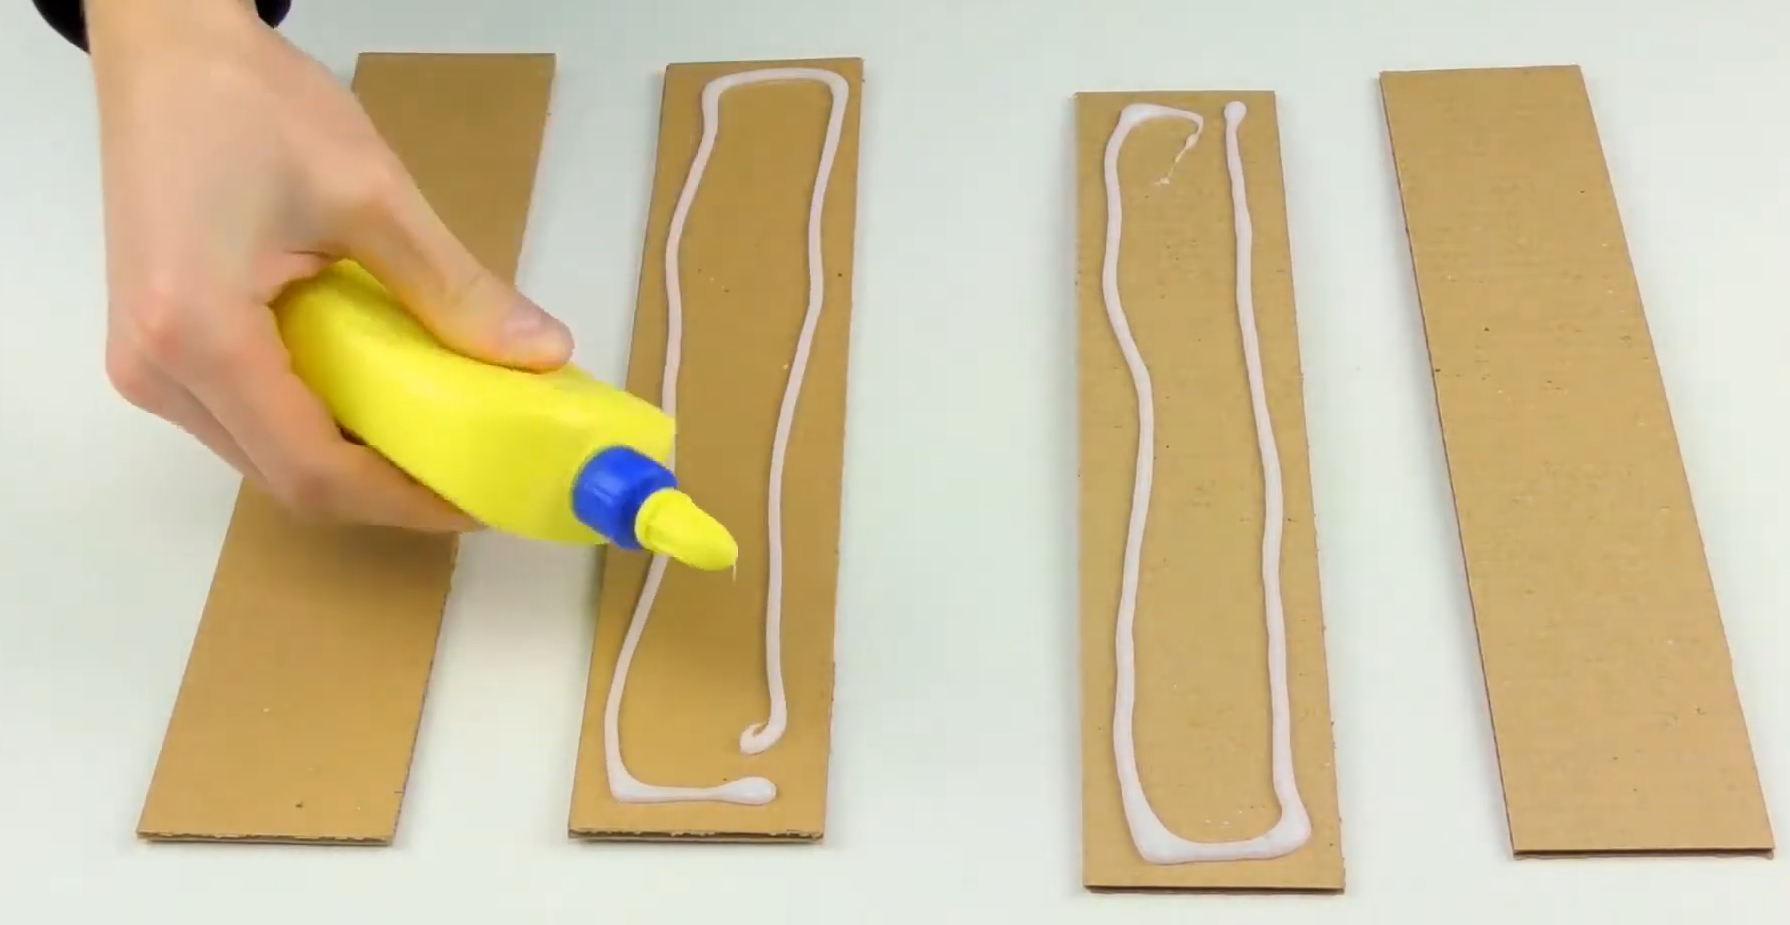
\includegraphics[width= 0.8\linewidth]{4}
		
		\vspace*{1pt}
		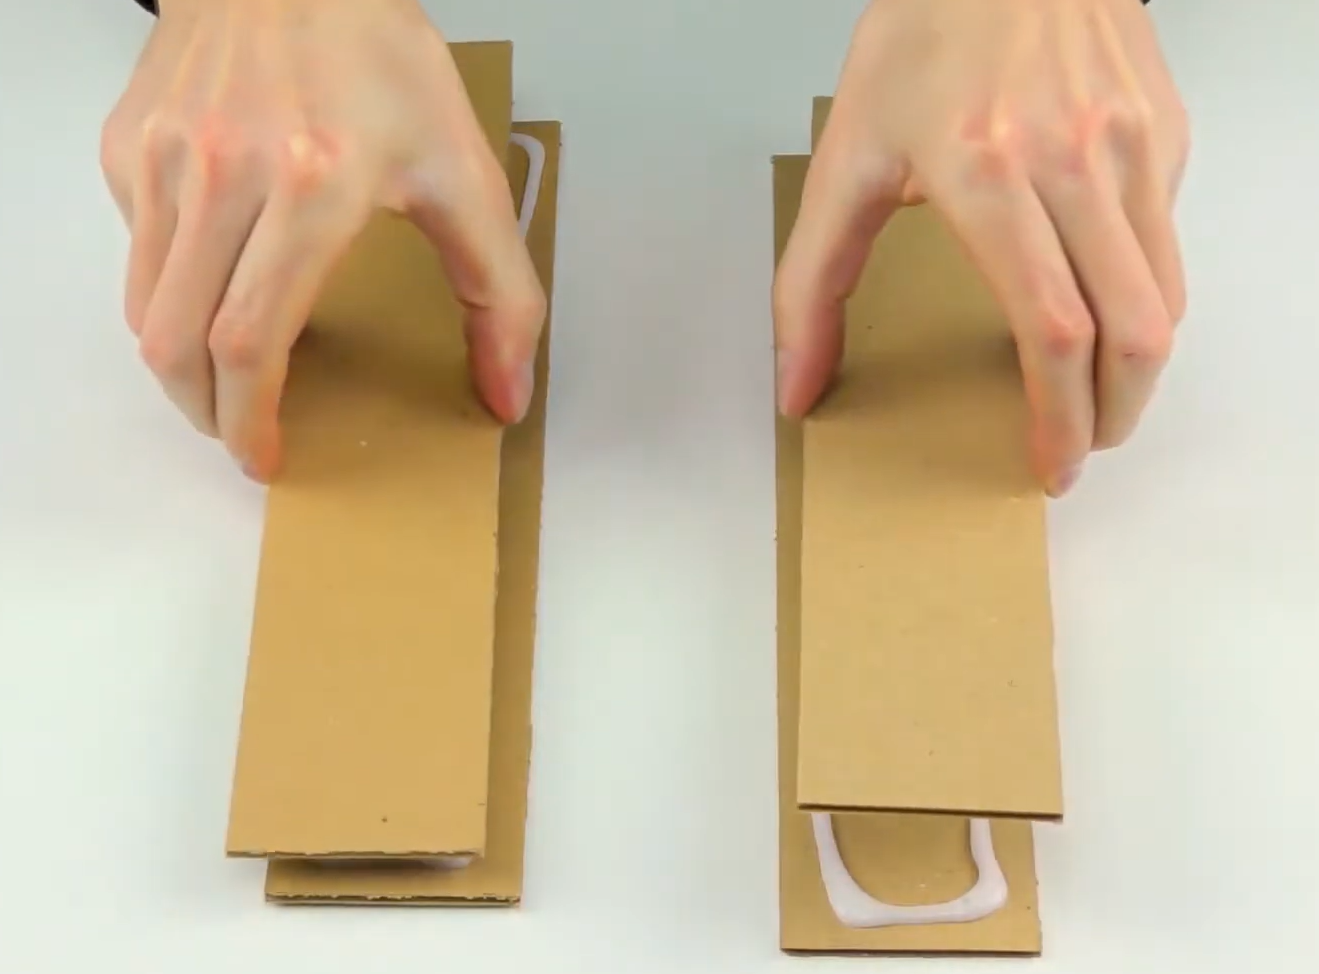
\includegraphics[width= 0.8\linewidth]{5}
		\vspace*{-10pt}
	\end{figure}
	\textbf{\color{toancuabi}Bước $\pmb{4}$:} Vẽ một hình vuông nhỏ lên phía trên của một miếng bìa giấy (miếng bìa giấy đó có kích thước $6$cm $\times$ $41$cm) rồi dùng dao rọc giấy cắt đi miếng hình vuông nhỏ đó. 
	\begin{figure}[H]
		\vspace*{-5pt}
		\centering
		\captionsetup{labelformat= empty, justification=centering}
		
\includegraphics[width= 0.8\linewidth]{6}
		\vspace*{-5pt}
	\end{figure}
	\textbf{\color{toancuabi}Bước $\pmb{5}$:} Sử dụng súng bắn keo để dán $4$ miếng bìa giấy nhỏ xung quanh miếng bìa giấy lớn.
	\begin{figure}[H]
		\vspace*{-5pt}
		\centering
		\captionsetup{labelformat= empty, justification=centering}
		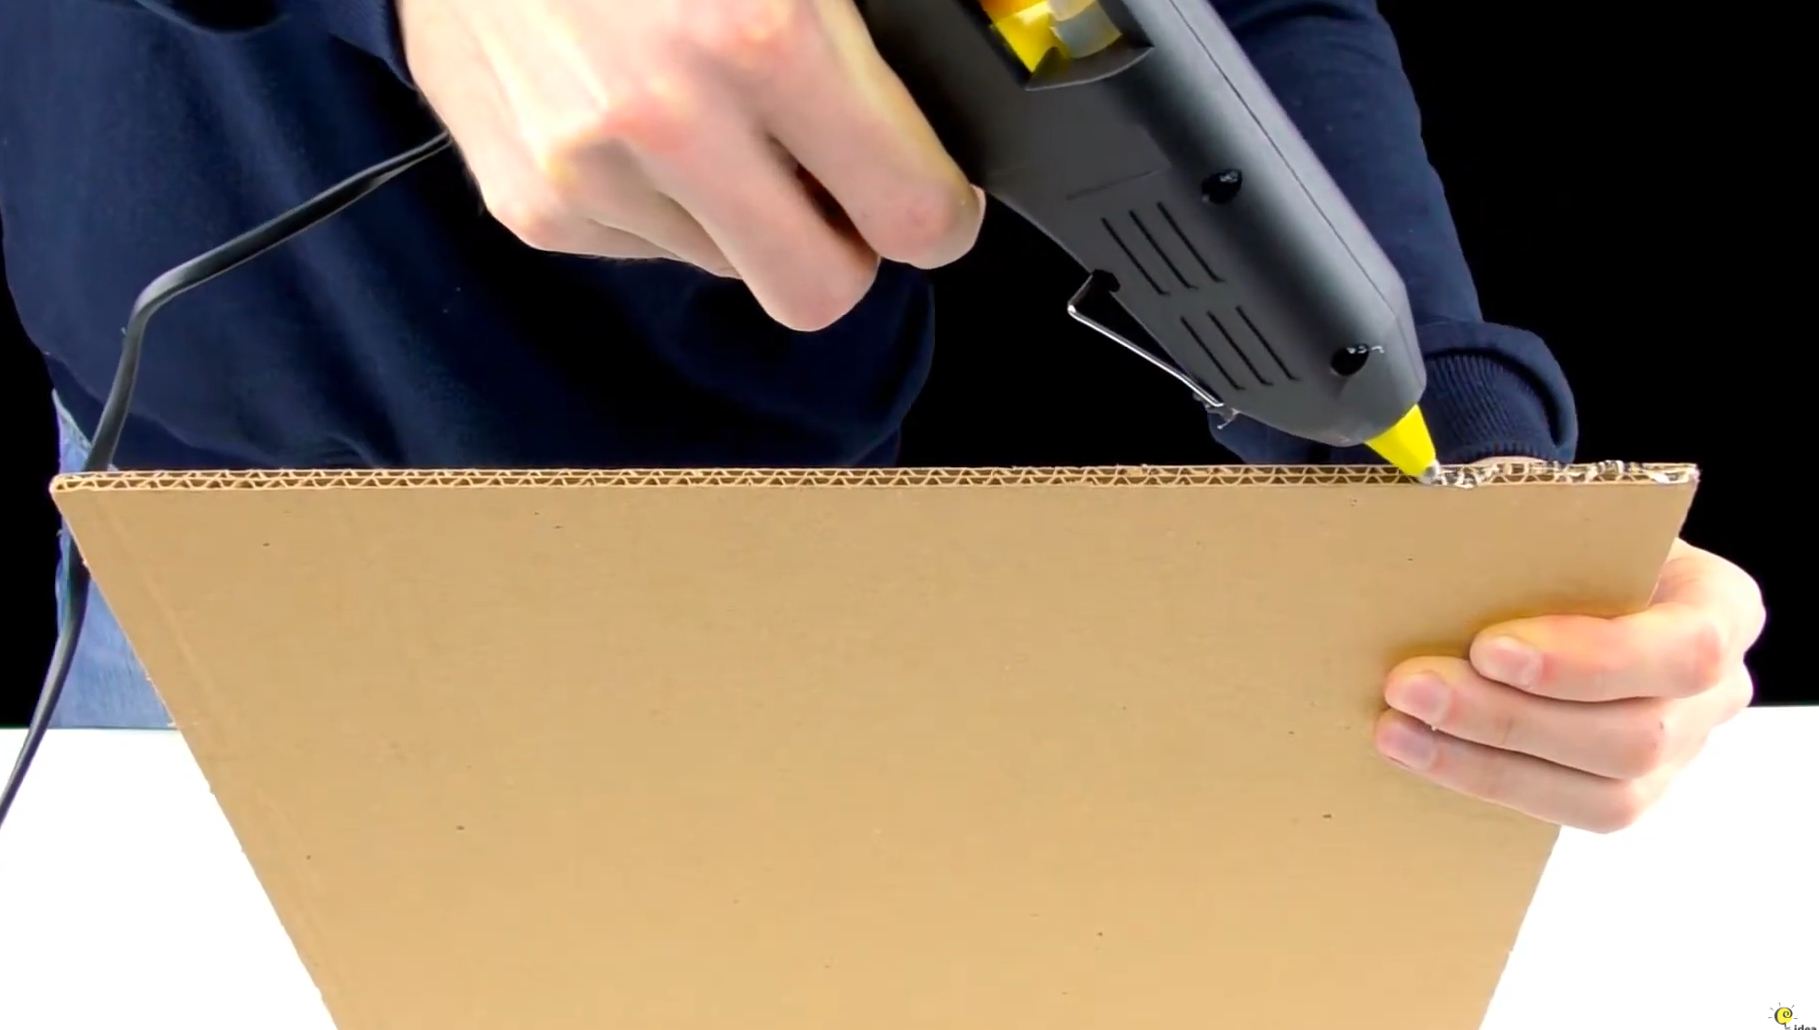
\includegraphics[width= 0.8\linewidth]{7}
		
		\vspace*{1pt}
		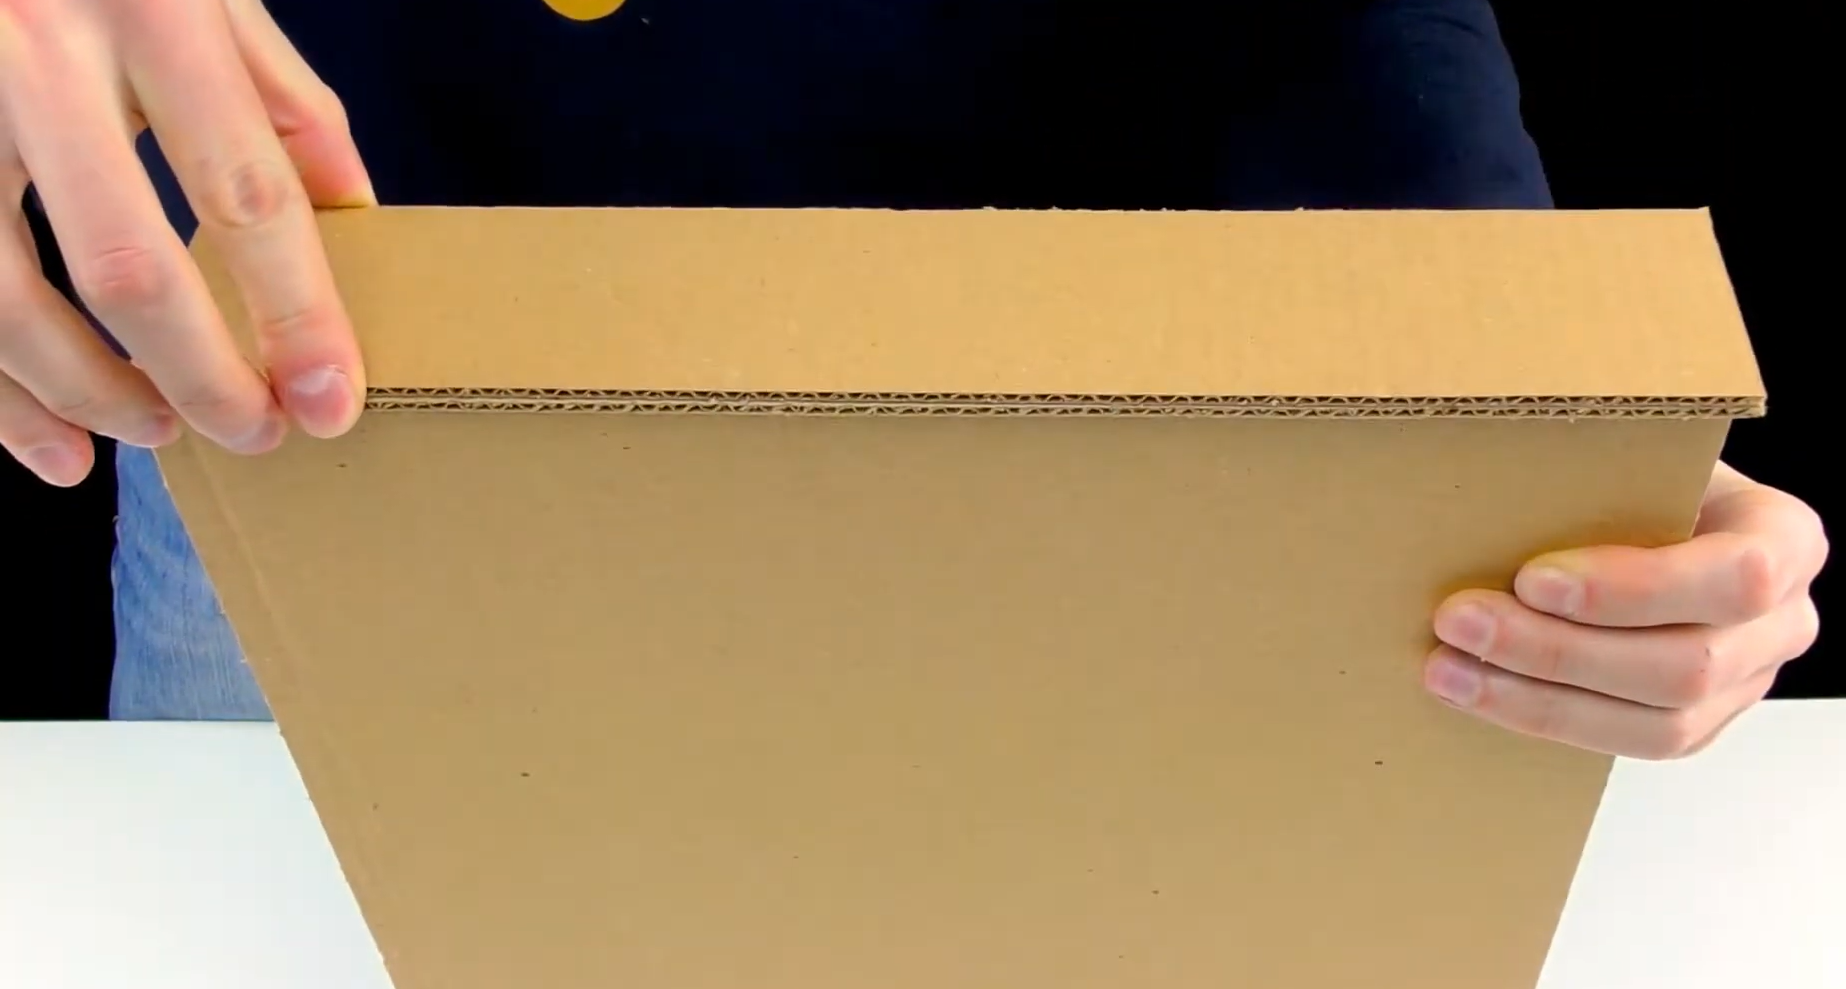
\includegraphics[width= 0.8\linewidth]{8}
		
		\vspace*{1pt}
		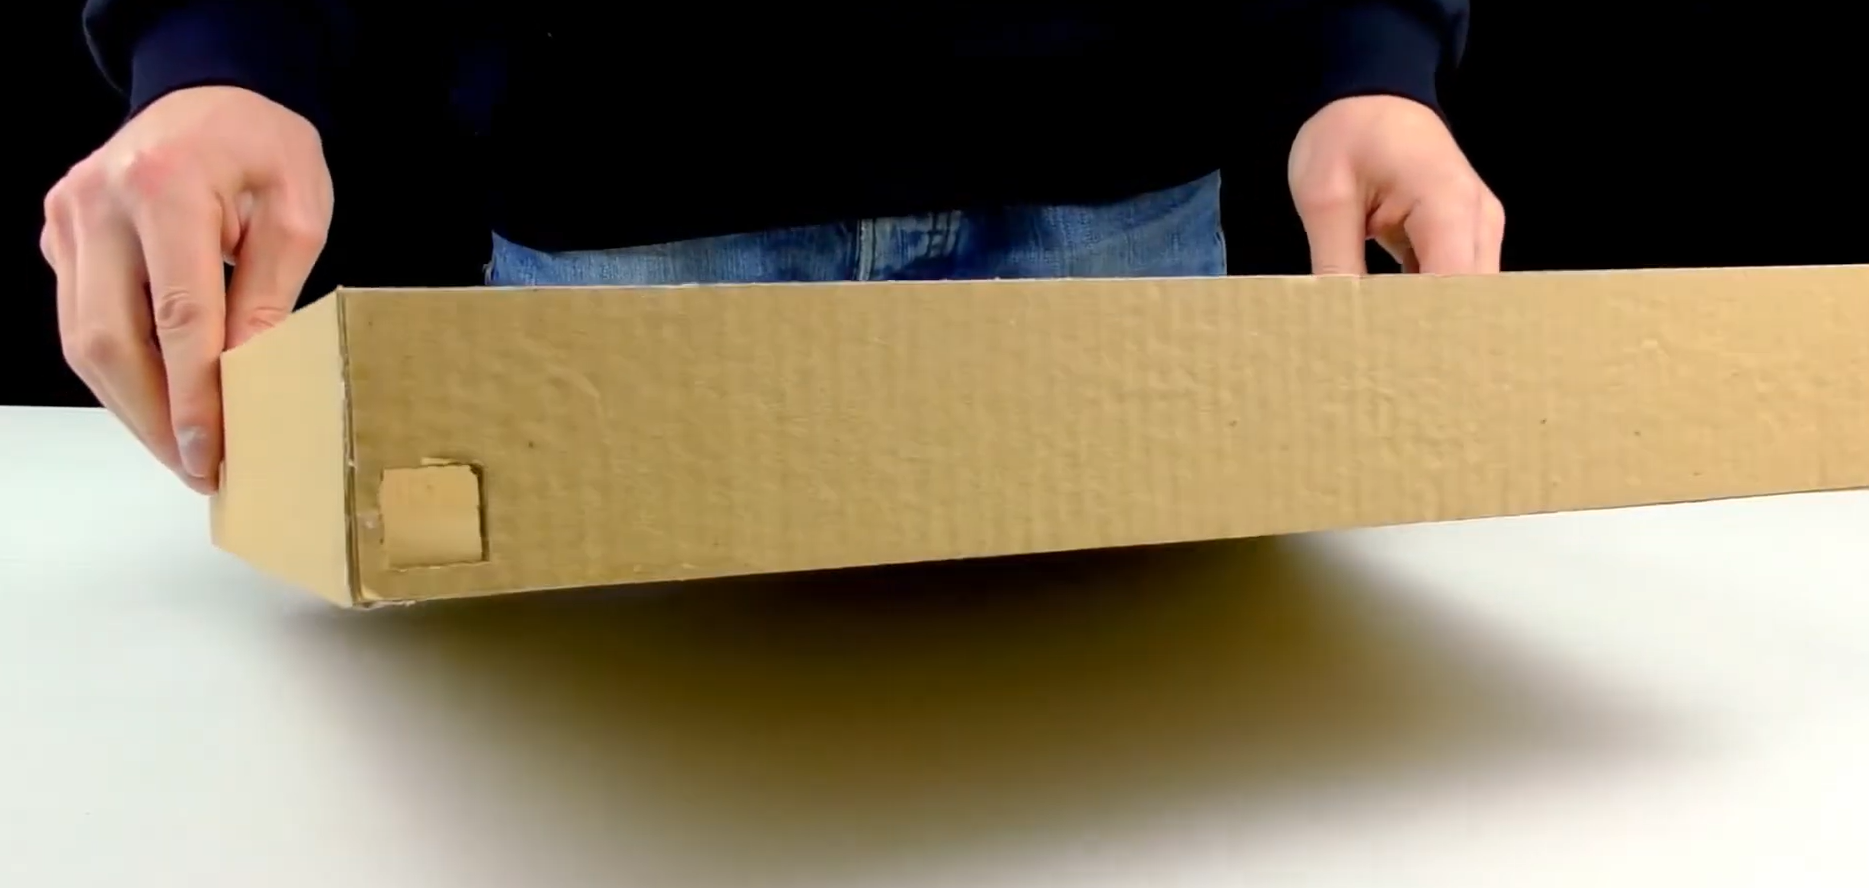
\includegraphics[width= 0.8\linewidth]{9}
		\vspace*{-10pt}
	\end{figure}
	\textbf{\color{toancuabi}Bước $\pmb{6}$:} Tiếp tục cắt các miếng bìa giấy hình chữ nhật có kích thước như hình bên dưới (đơn vị: cm).
	\begin{figure}[H]
		\vspace*{-5pt}
		\centering
		\captionsetup{labelformat= empty, justification=centering}
		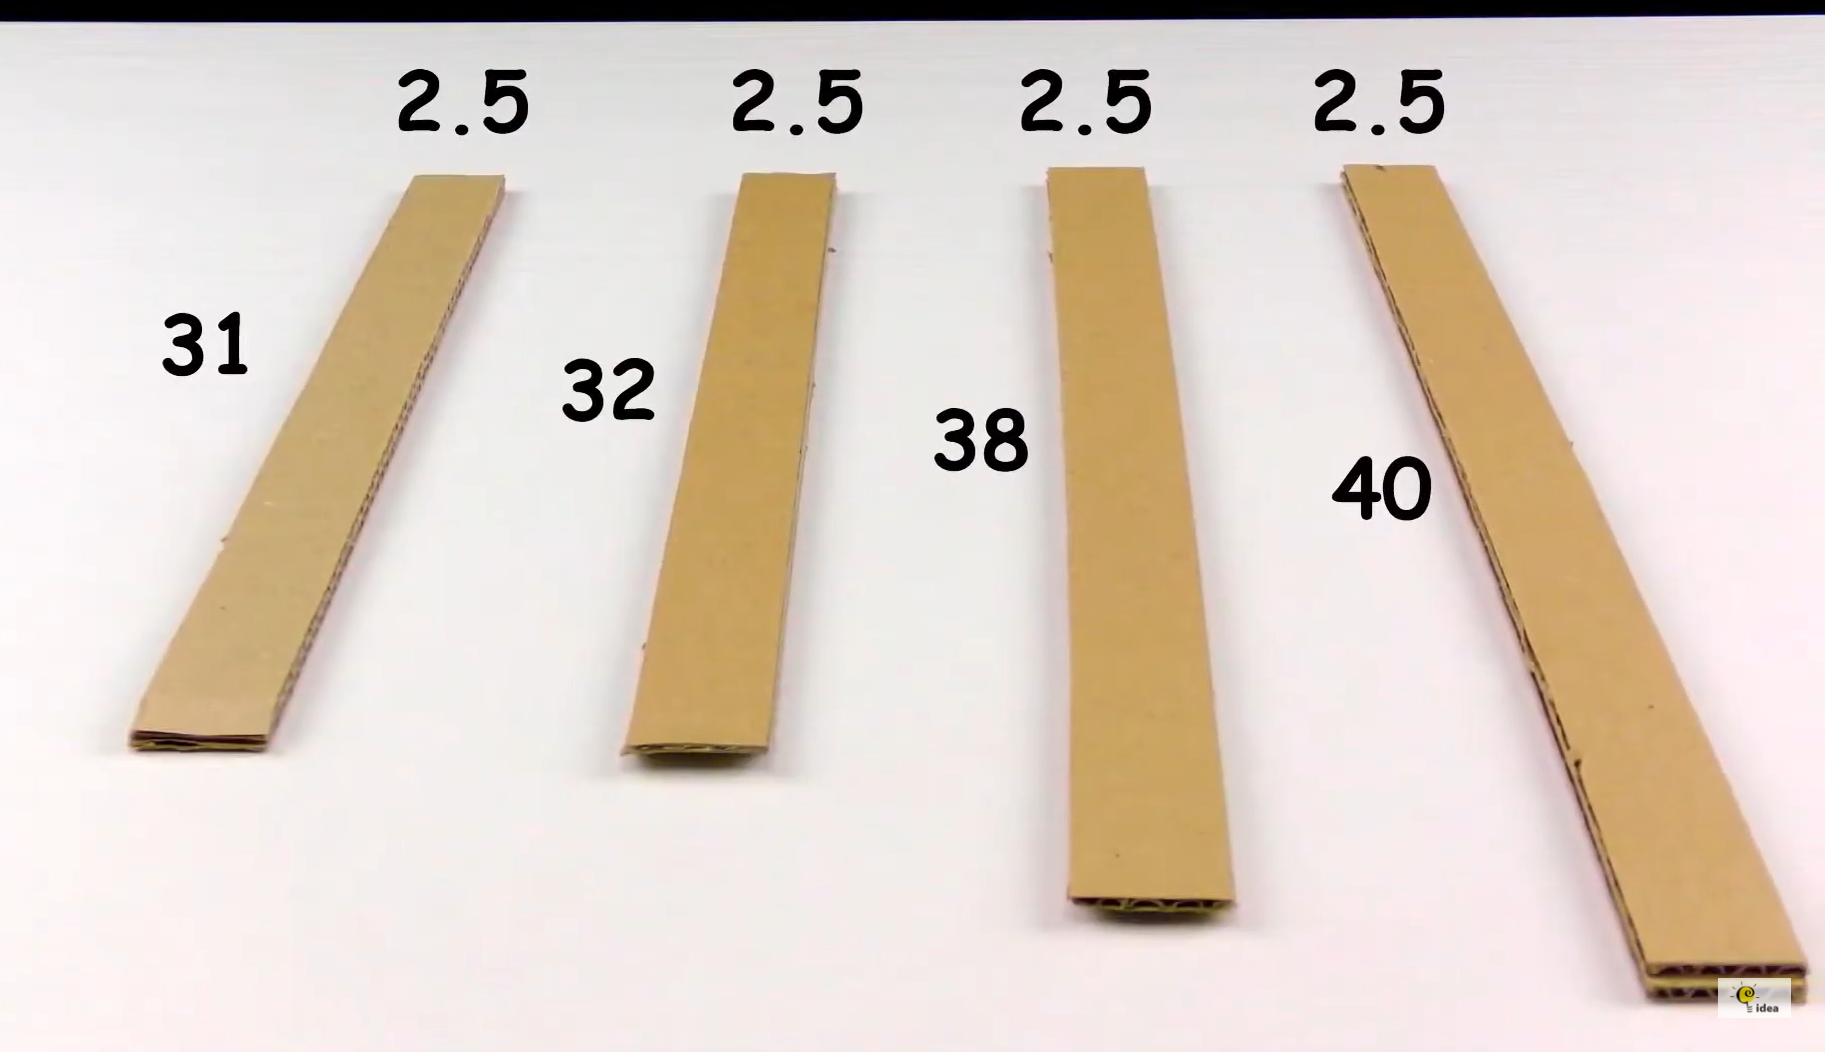
\includegraphics[width= 0.8\linewidth]{10}
		\vspace*{-10pt}
	\end{figure}
	\textbf{\color{toancuabi}Bước $\pmb{7}$:} Dán các miếng bìa nhỏ này (đã được làm dày gấp đôi tương tự như ở bước $2$) vào xung quanh phần bên trong hộp.
	\begin{figure}[H]
		\vspace*{-5pt}
		\centering
		\captionsetup{labelformat= empty, justification=centering}
		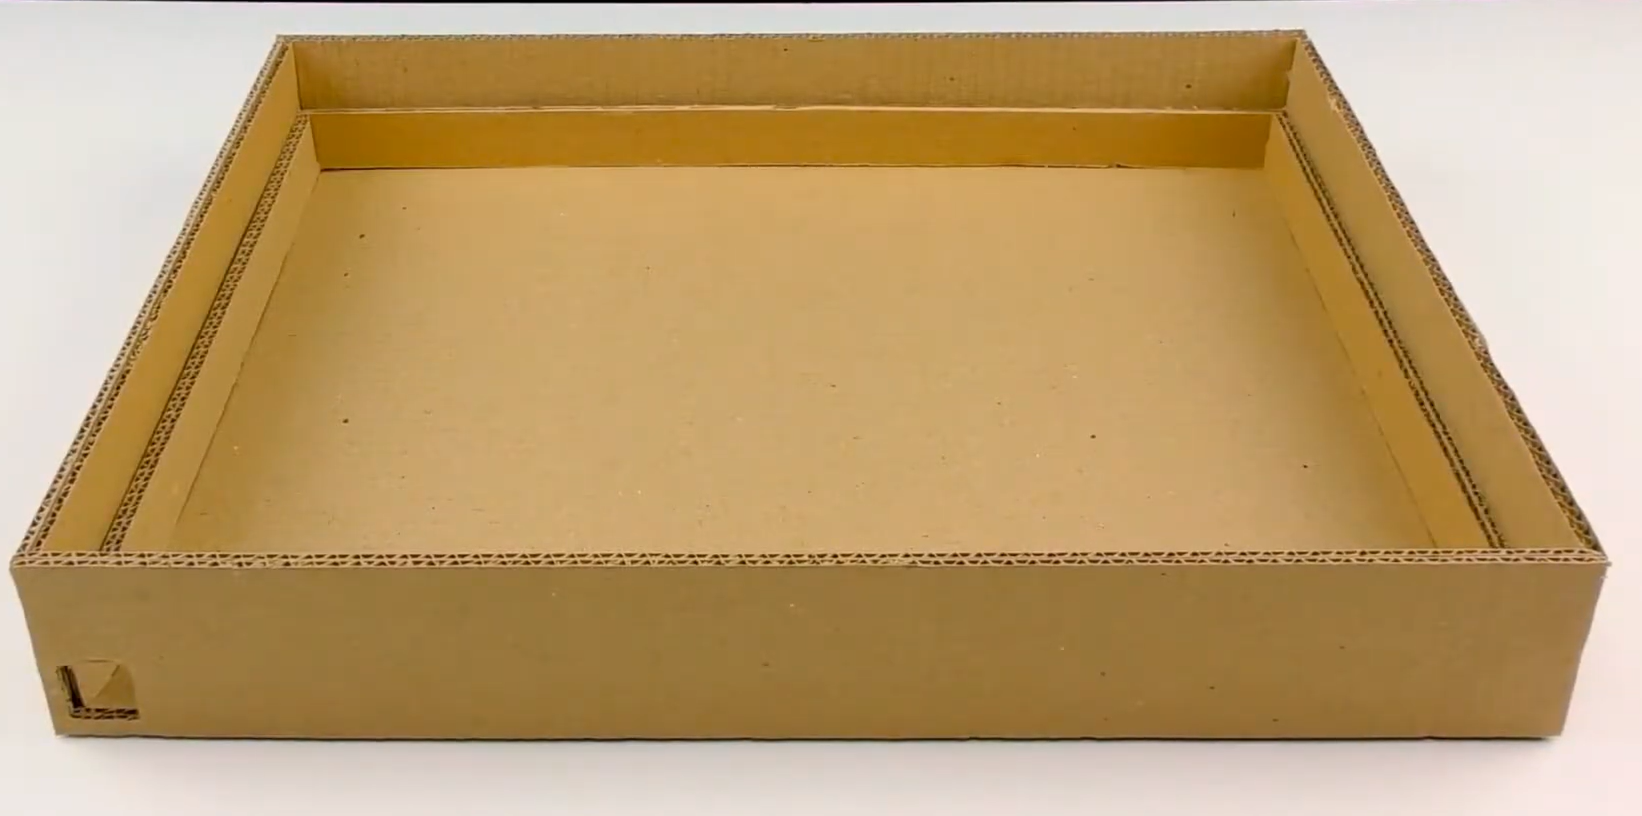
\includegraphics[width= 0.8\linewidth]{11}
		\vspace*{-10pt}
	\end{figure}
	\textbf{\color{toancuabi}Bước $\pmb{8}$:} Vẽ mê cung vào tấm bìa hình chữ nhật có kích thước $32$cm $\times$ $39$cm.
	\begin{figure}[H]
		\vspace*{5pt}
		\centering
		\captionsetup{labelformat= empty, justification=centering}
		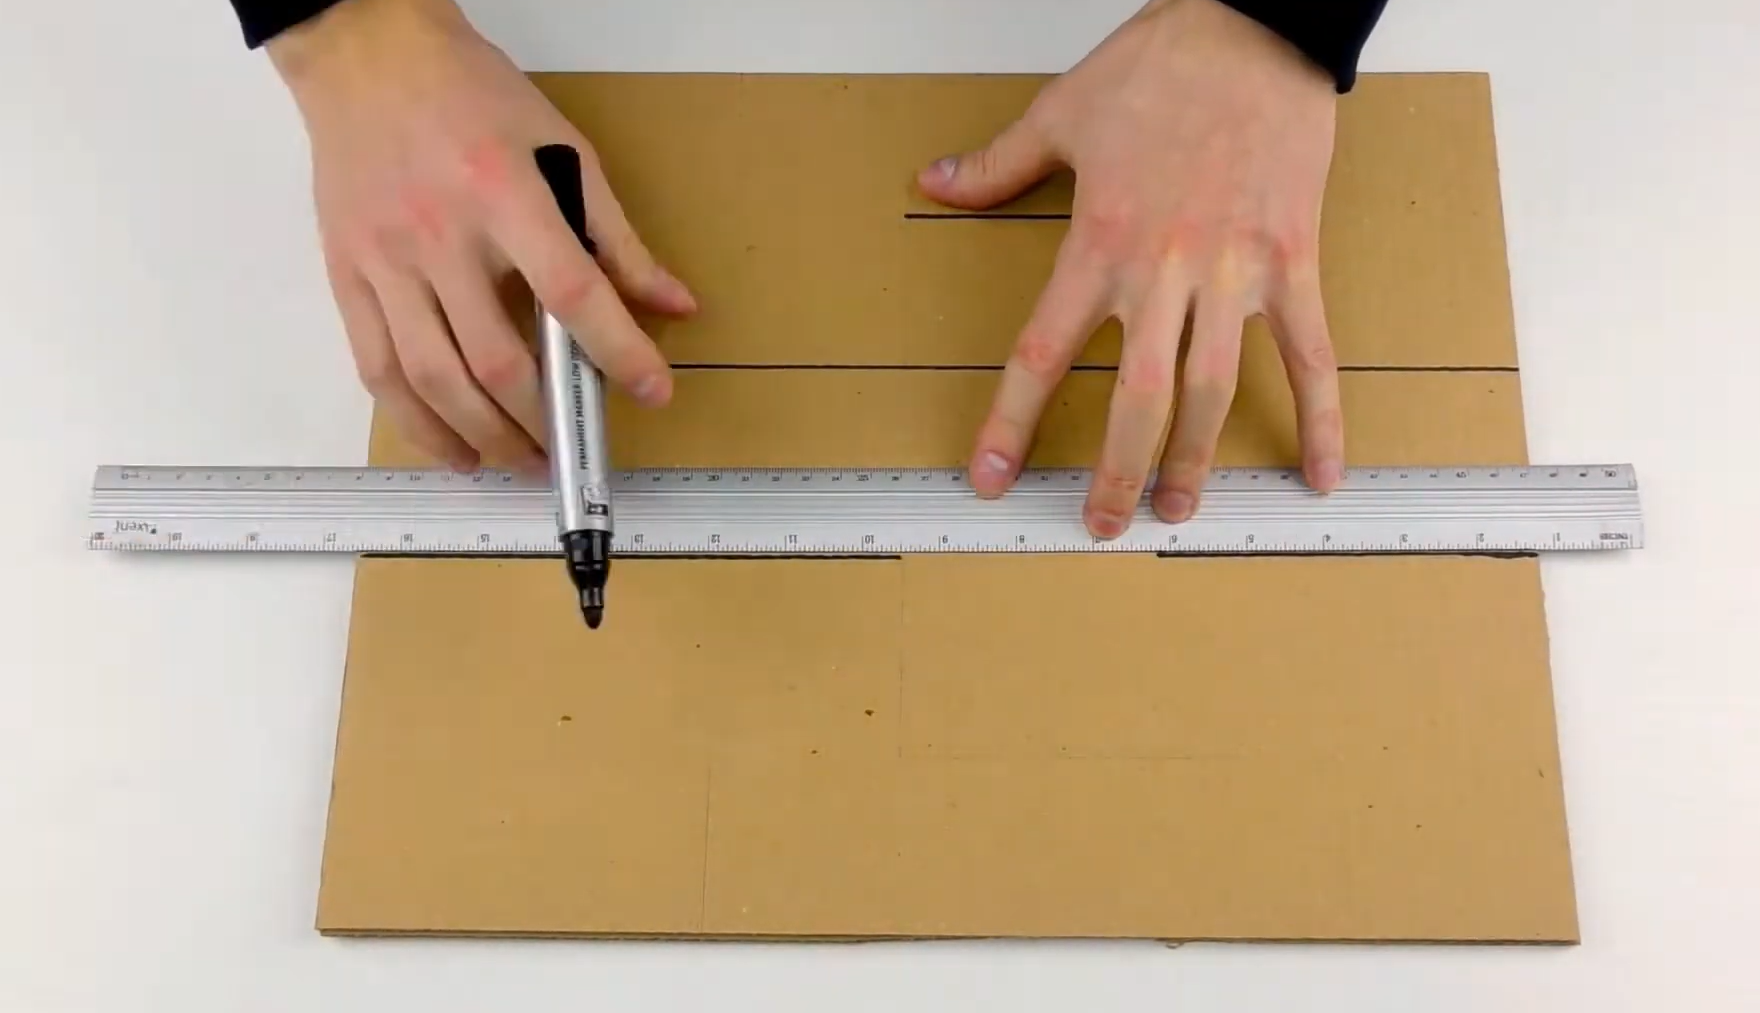
\includegraphics[width= 0.8\linewidth]{12}
		
		\vspace*{1pt}
		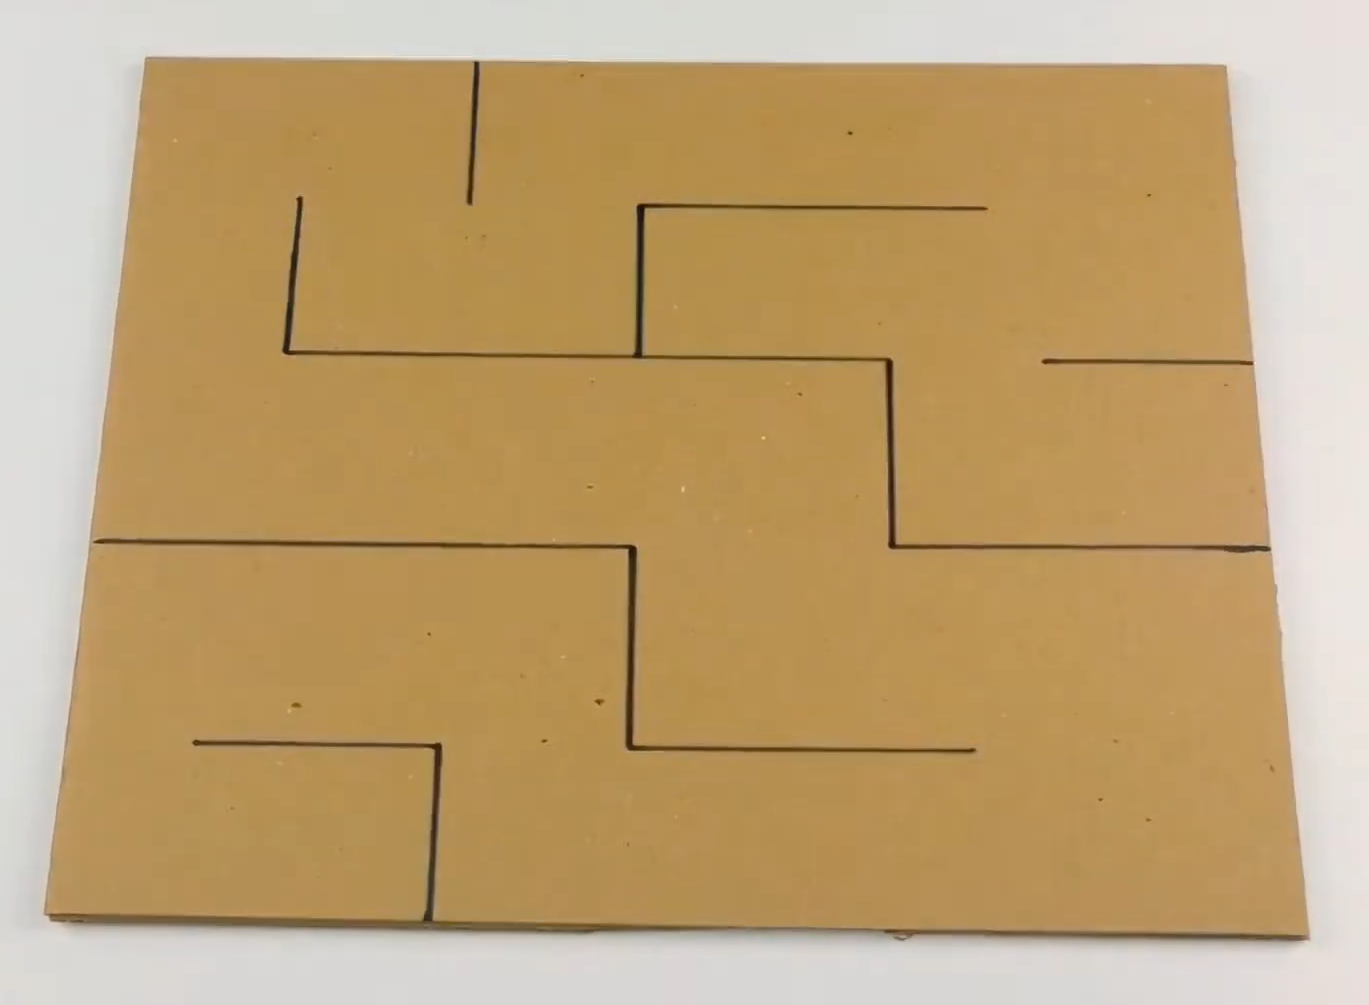
\includegraphics[width= 0.8\linewidth]{13}
		\vspace*{-10pt}
	\end{figure}
	\textbf{\color{toancuabi}Bước $\pmb{9}$:} Sử dụng lõi keo dán hoặc com-pa để vẽ các hình tròn như hình minh họa bên dưới, sau đó dùng dao rọc giấy cắt đi các hình tròn.
	\begin{figure}[H]
		\vspace*{-5pt}
		\centering
		\captionsetup{labelformat= empty, justification=centering}
		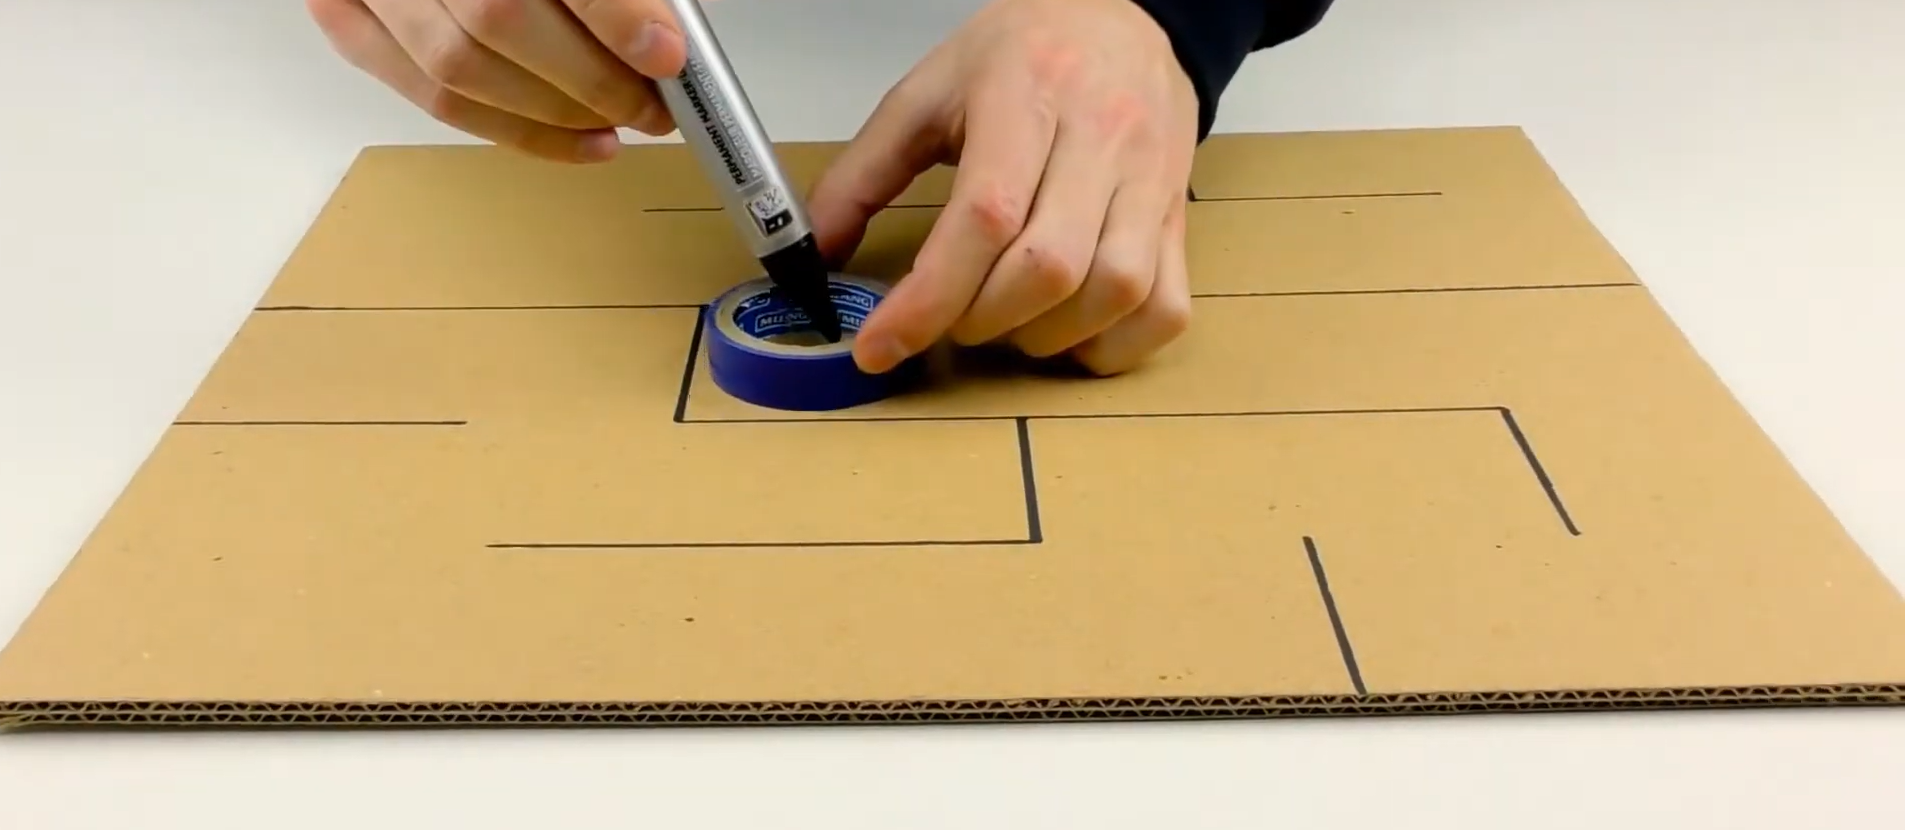
\includegraphics[width= 0.8\linewidth]{14}
		
		\vspace*{1pt}
		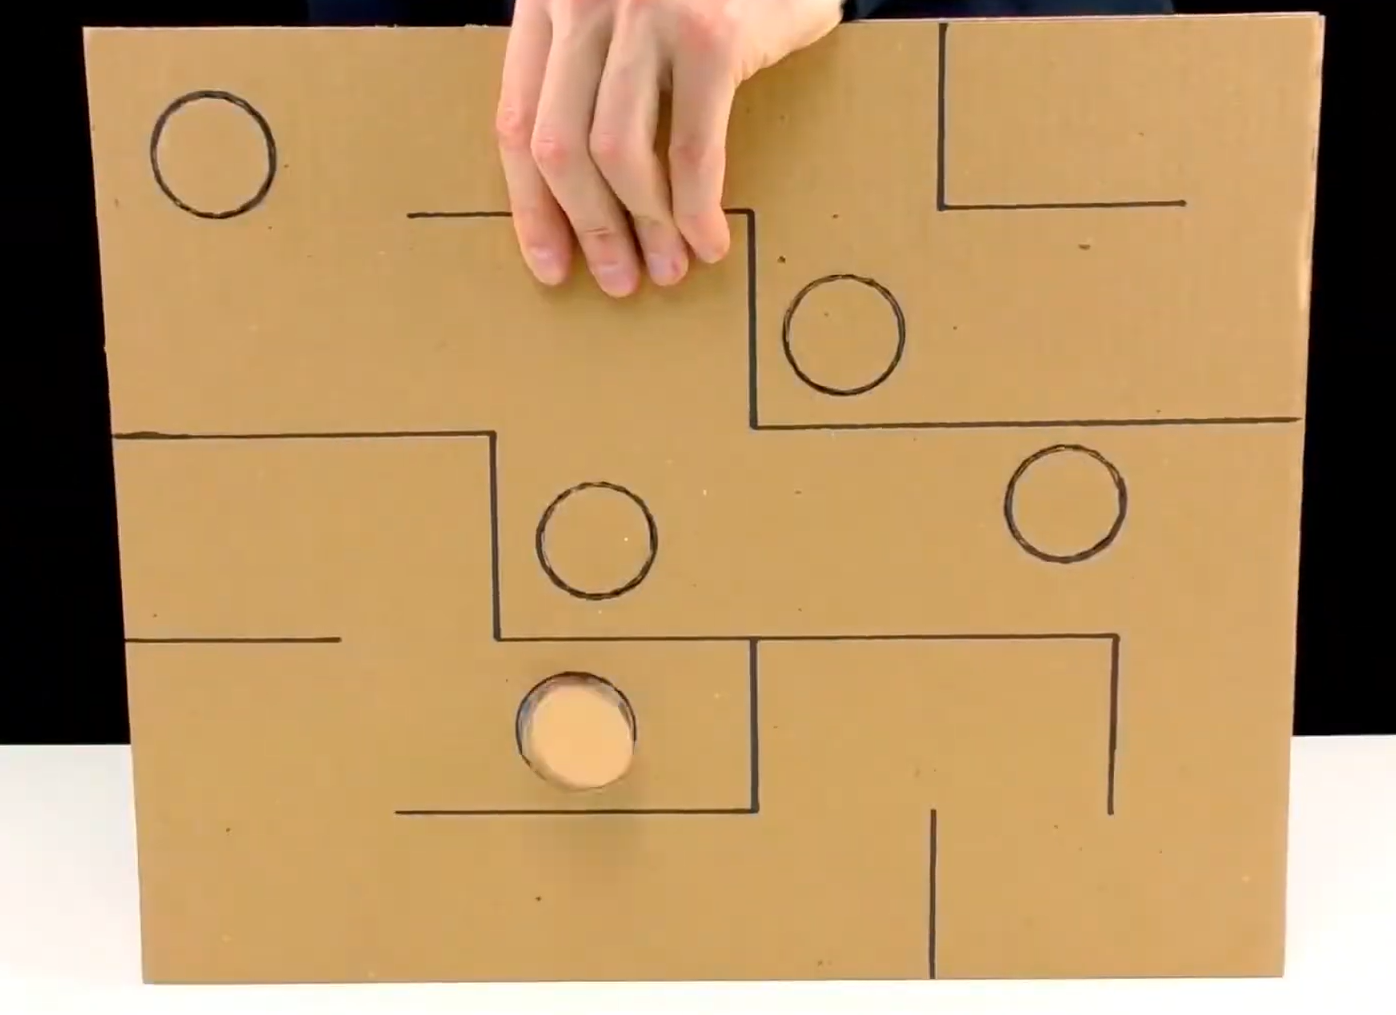
\includegraphics[width= 0.8\linewidth]{15}
		\vspace*{-10pt}
	\end{figure}
	\textbf{\color{toancuabi}Bước $\pmb{10}$:} Dán các miếng bìa giấy nhỏ lên mê cung như hình minh họa.
	\begin{figure}[H]
		\vspace*{-5pt}
		\centering
		\captionsetup{labelformat= empty, justification=centering}
		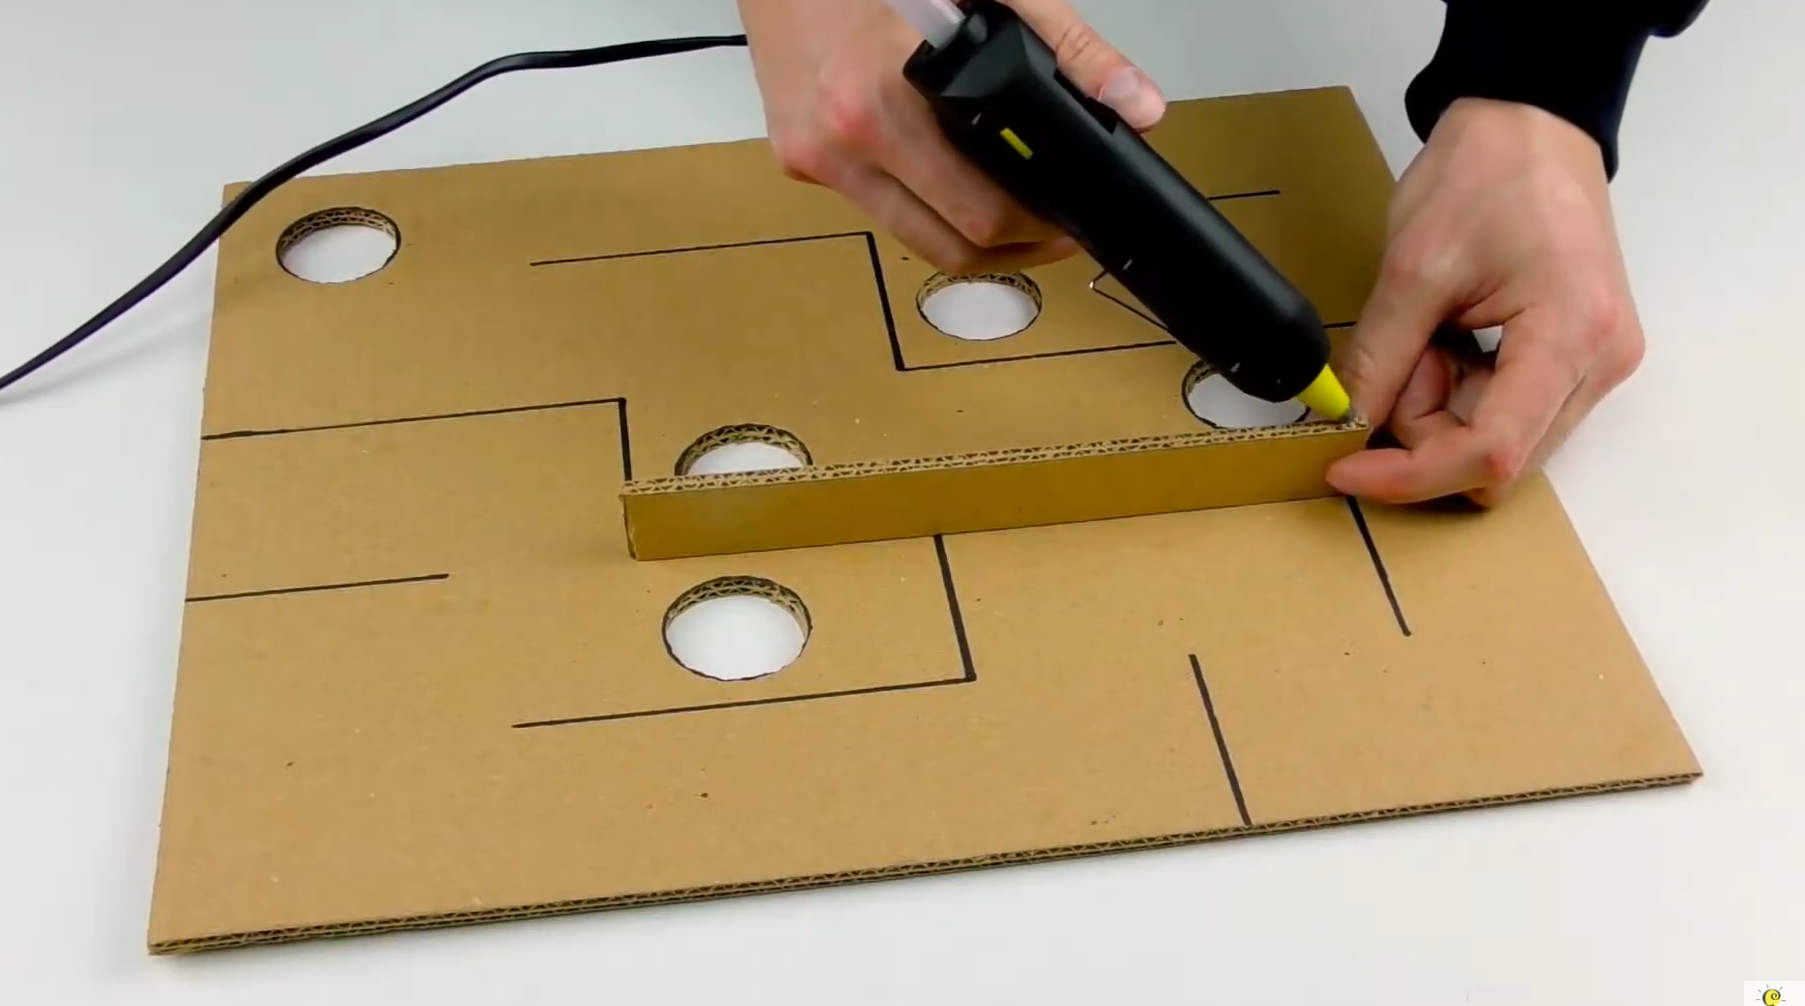
\includegraphics[width= 0.8\linewidth]{16}
%		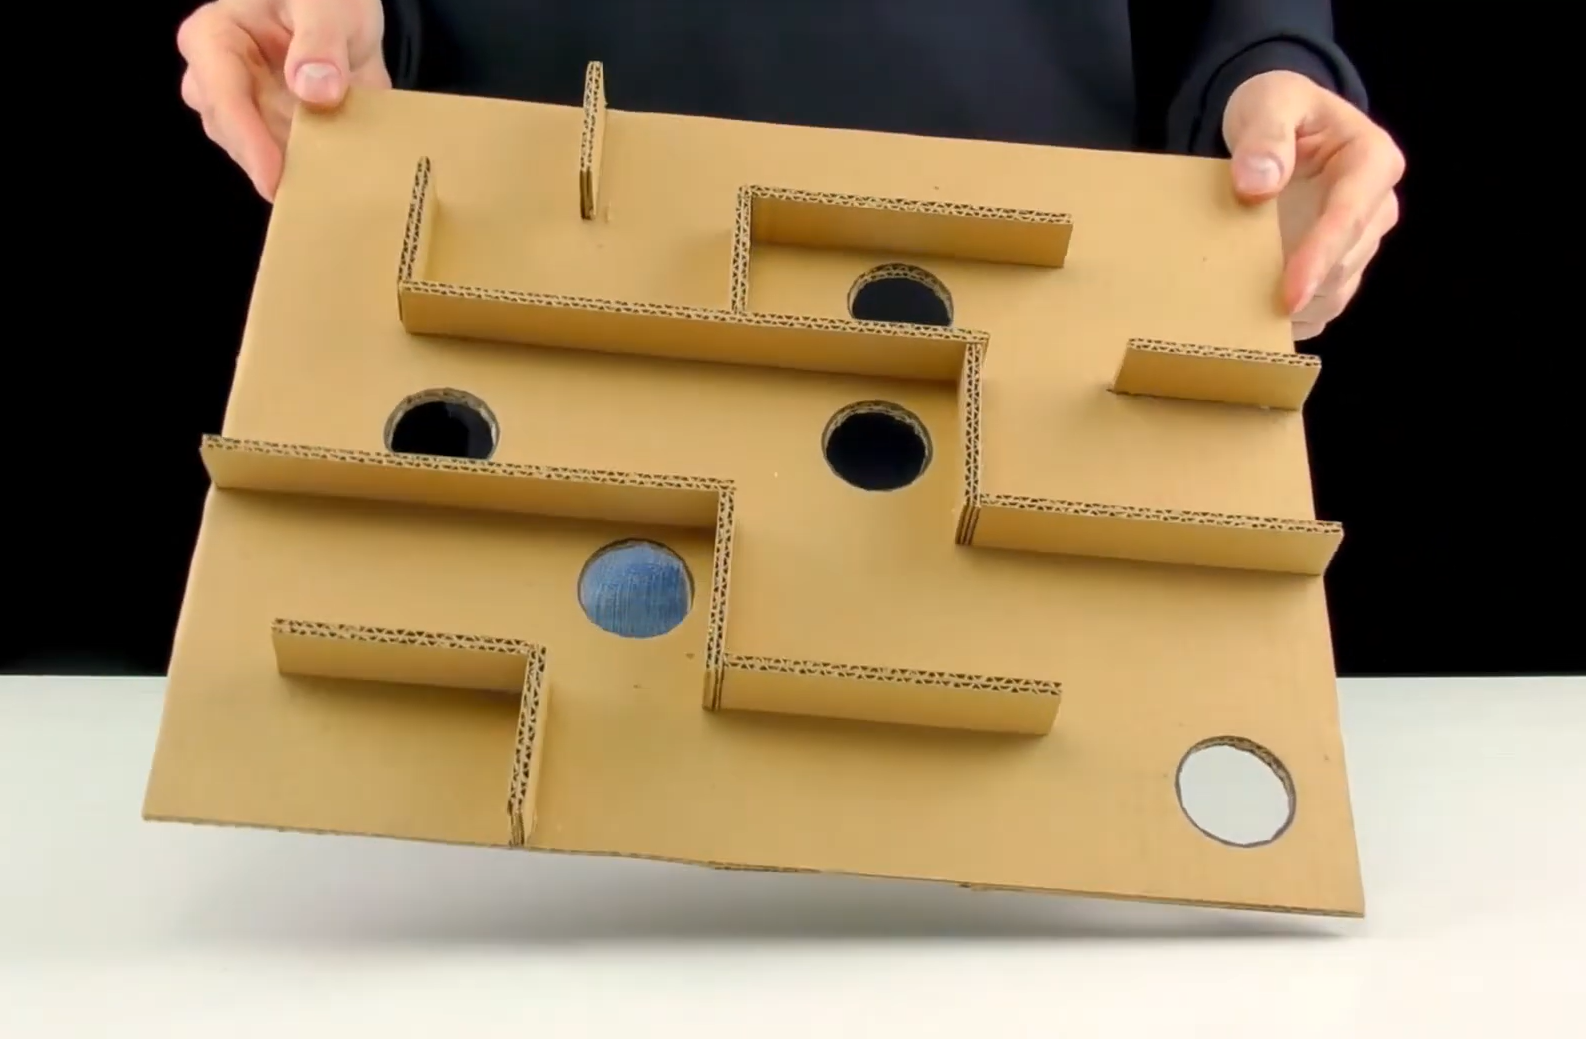
\includegraphics[width= 0.8\linewidth]{17}
		\vspace*{-5pt}
	\end{figure}
		\begin{figure}[H]
		\vspace*{5pt}
		\centering
		\captionsetup{labelformat= empty, justification=centering}
%		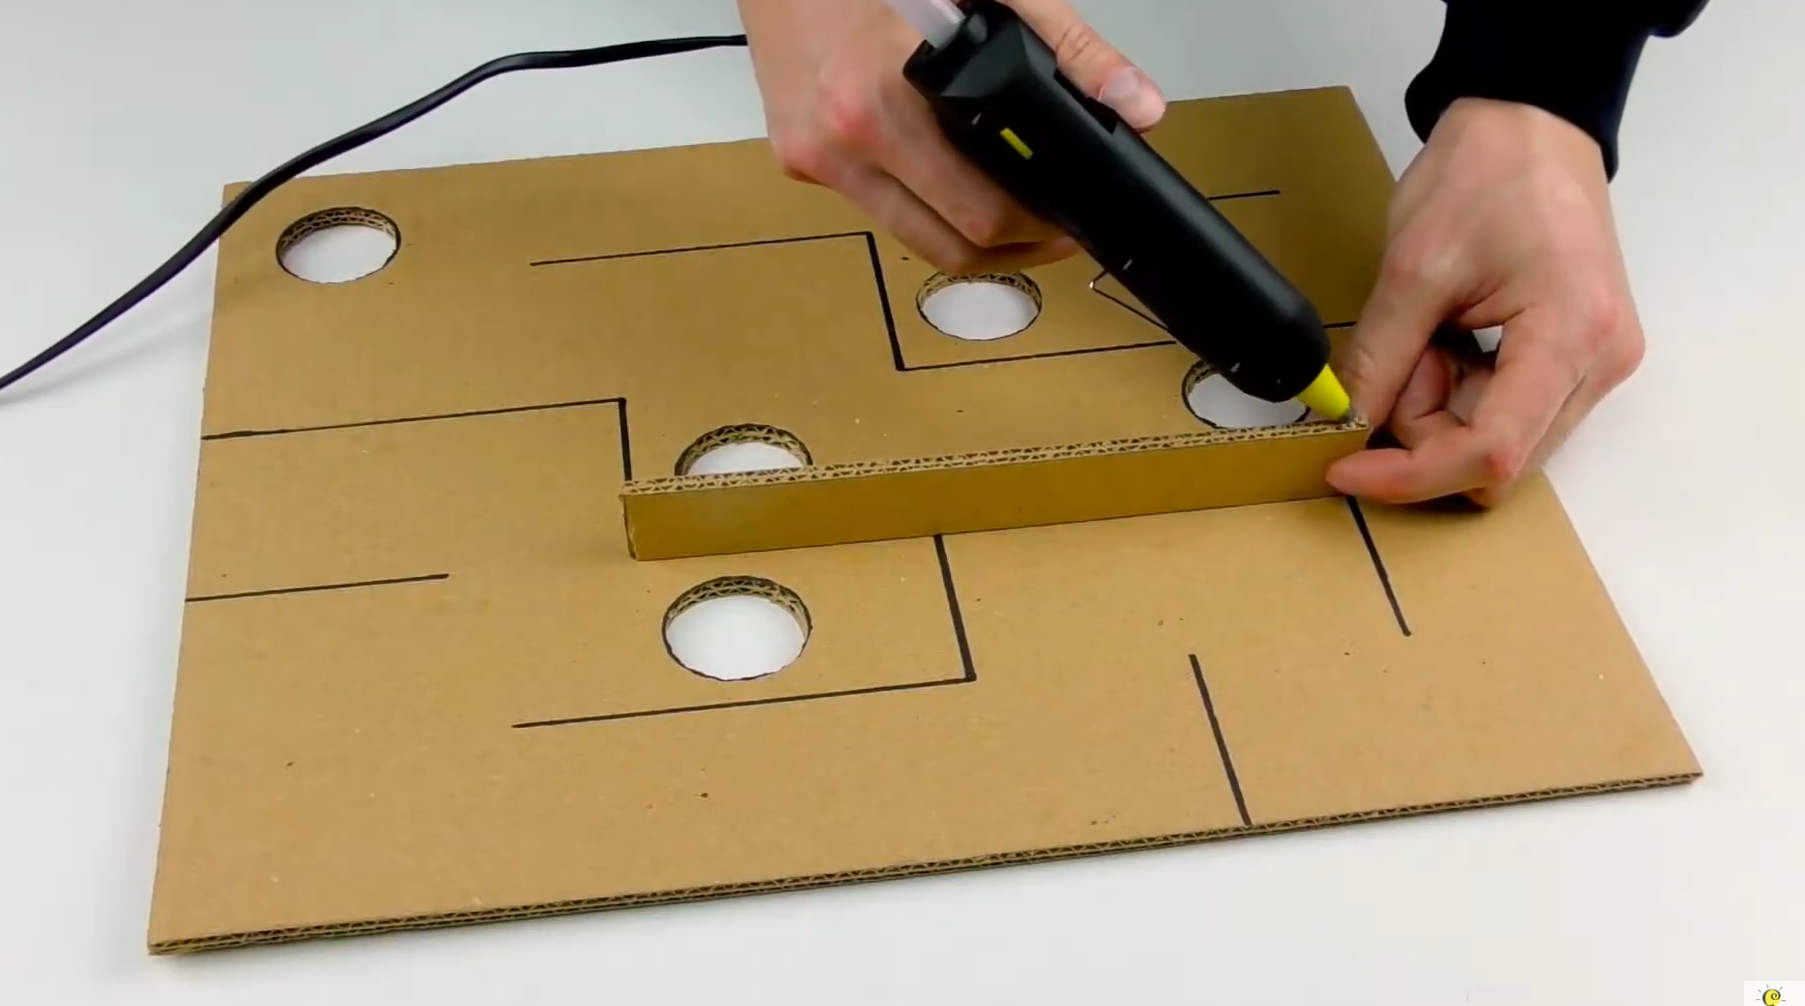
\includegraphics[width= 0.8\linewidth]{16}
		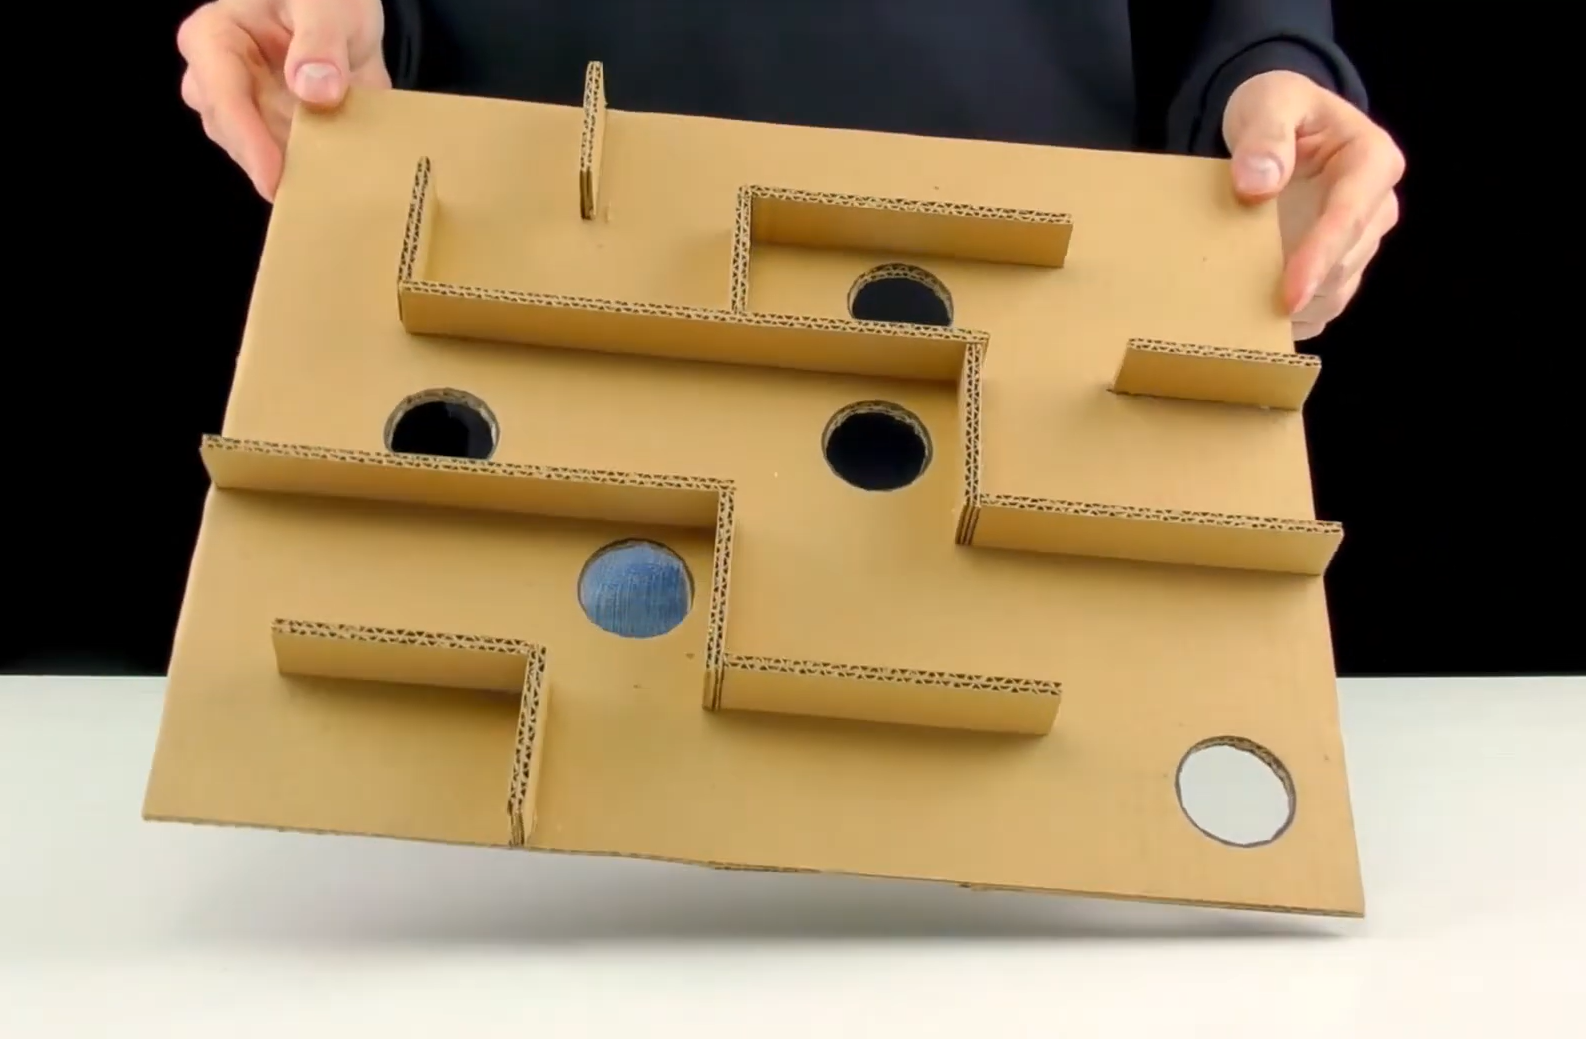
\includegraphics[width= 0.8\linewidth]{17}
		\vspace*{-10pt}
	\end{figure}
	\textbf{\color{toancuabi}Bước $\pmb{11}$:} Tiếp tục dán $4$ miếng bìa nhỏ xung quanh mê cung, dùng bút viết chữ START và FINISH ở vị trí như hình minh họa, sau đó đặt mê cung vào trong hộp đã được làm ở bước $7$.
	\begin{figure}[H]
		\vspace*{-5pt}
		\centering
		\captionsetup{labelformat= empty, justification=centering}
		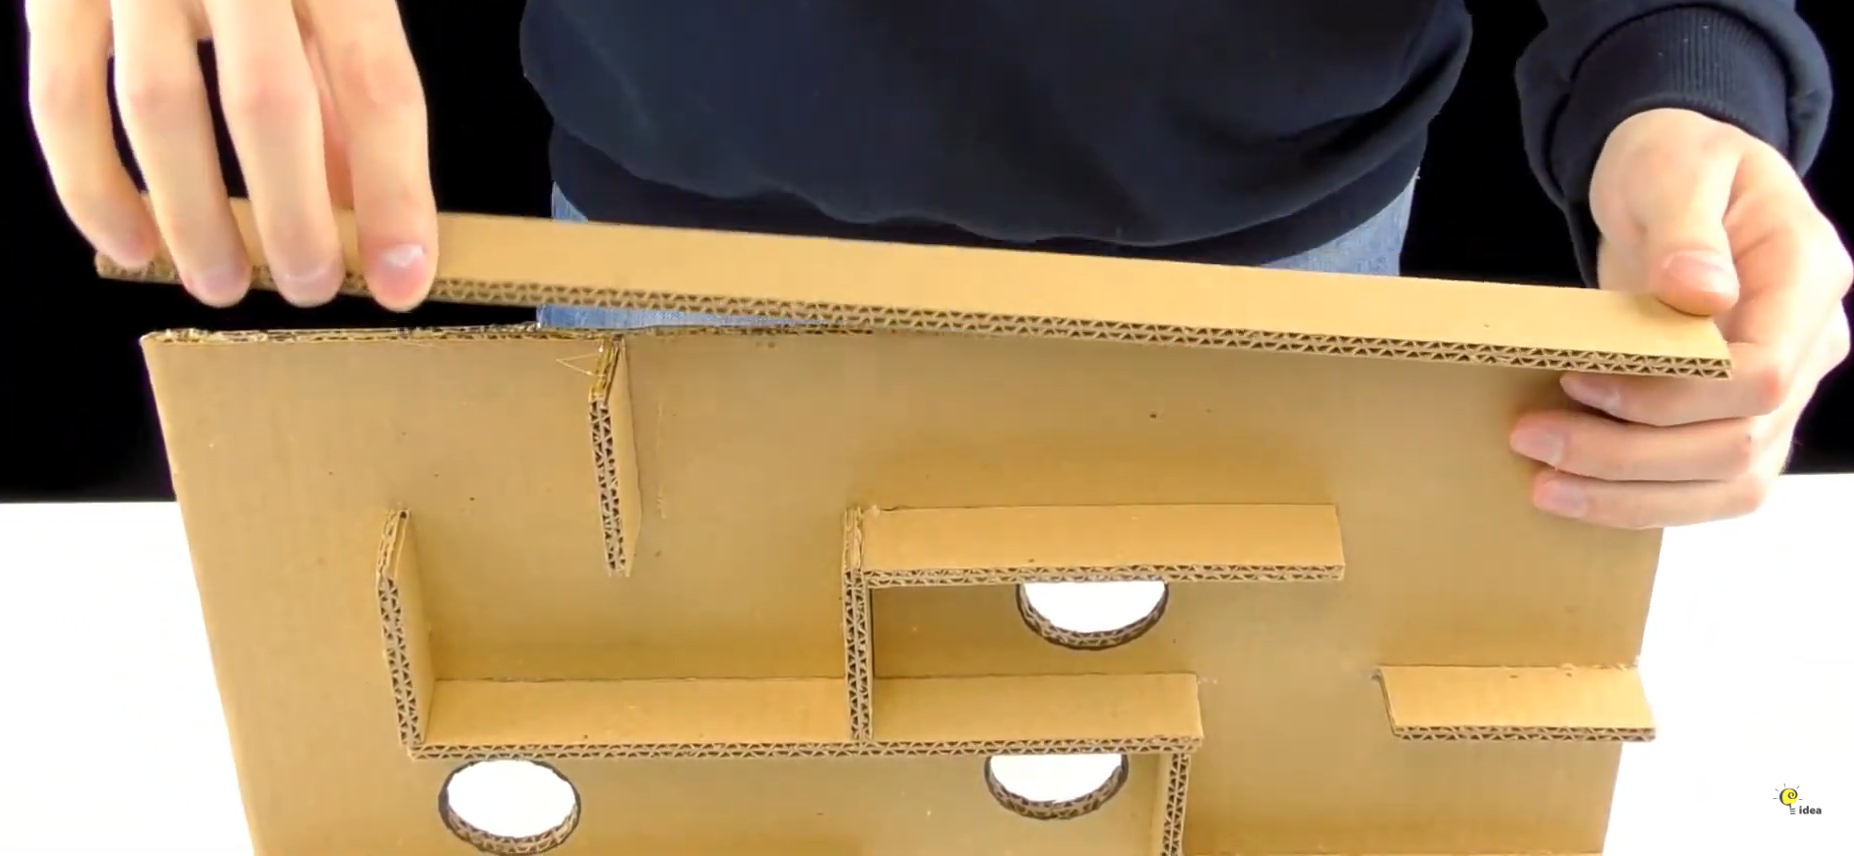
\includegraphics[width= 0.8\linewidth]{18}
		
		\vspace*{1pt}
		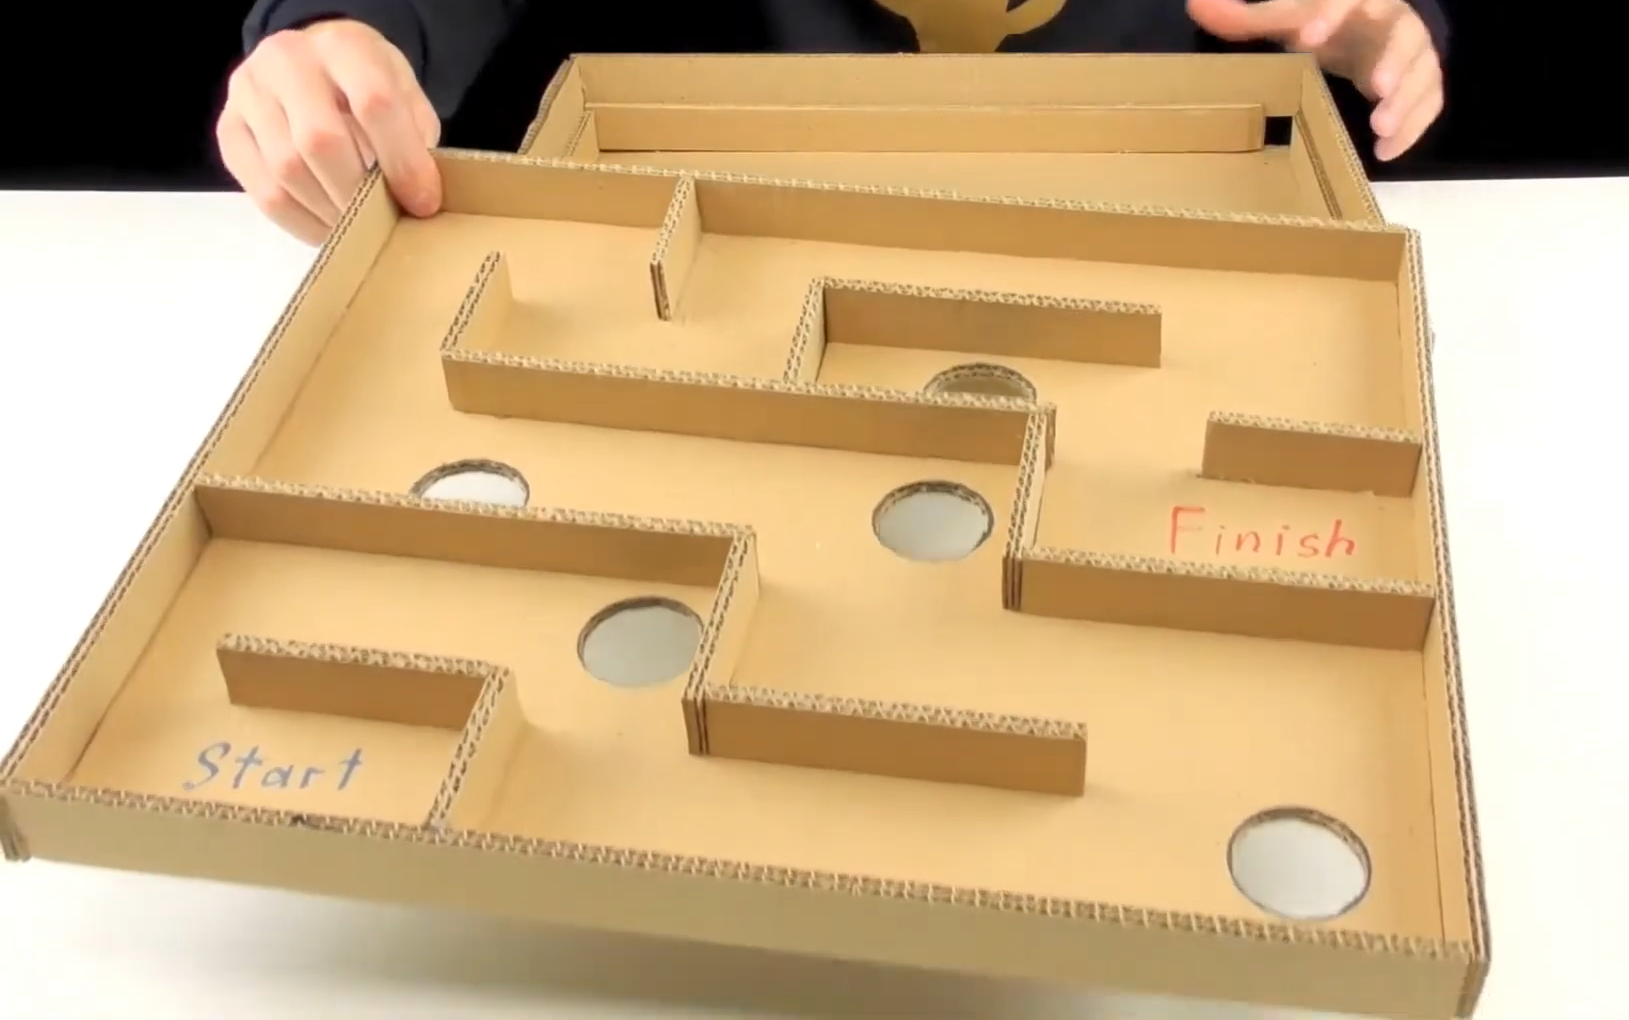
\includegraphics[width= 0.8\linewidth]{19}
		
		\vspace*{1pt}
		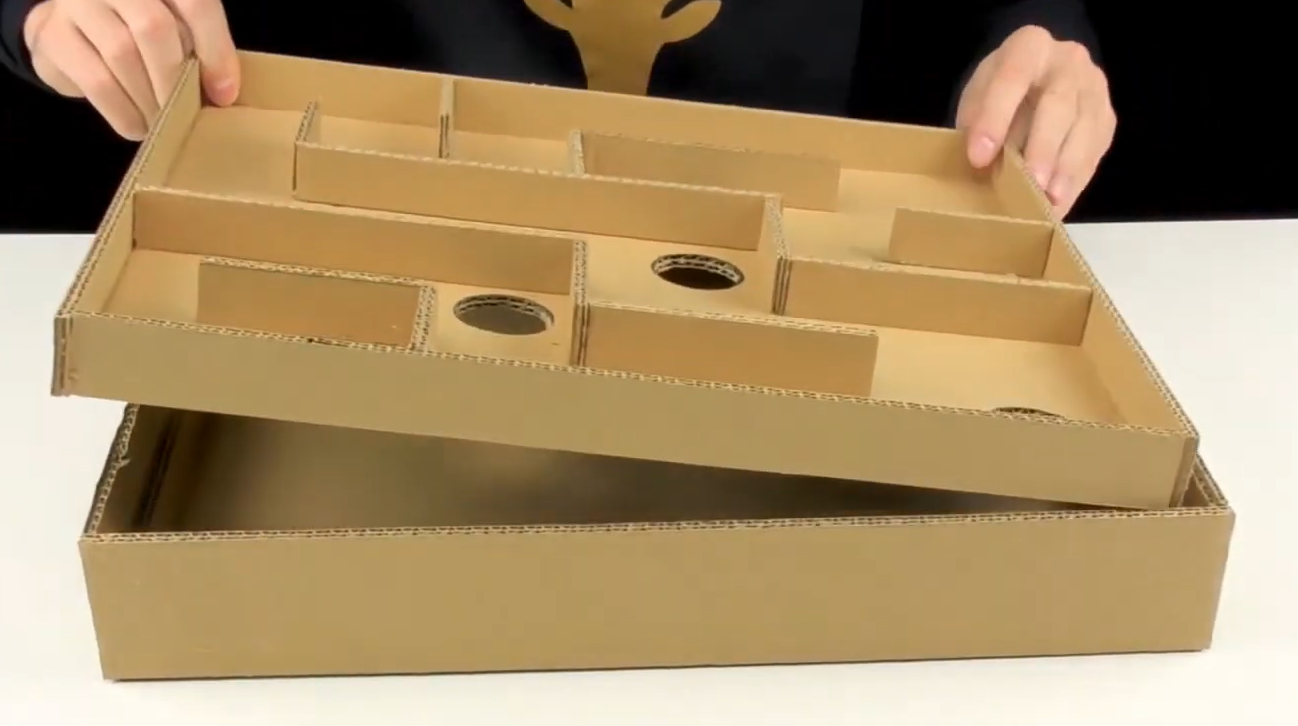
\includegraphics[width= 0.8\linewidth]{20}
		\vspace*{-10pt}
	\end{figure}
	\textbf{\color{toancuabi}Bước $\pmb{12}$:} Bỏ một viên bi vào vị trí START, nhiệm vụ của các em bây giờ là hãy di chuyển viên bi đến chữ FINISH. Các em hãy cẩn thận kẻo viên bi bị rơi xuống lỗ trên đường đi nhé!
	\begin{figure}[H]
		\vspace*{-5pt}
		\centering
		\captionsetup{labelformat= empty, justification=centering}
		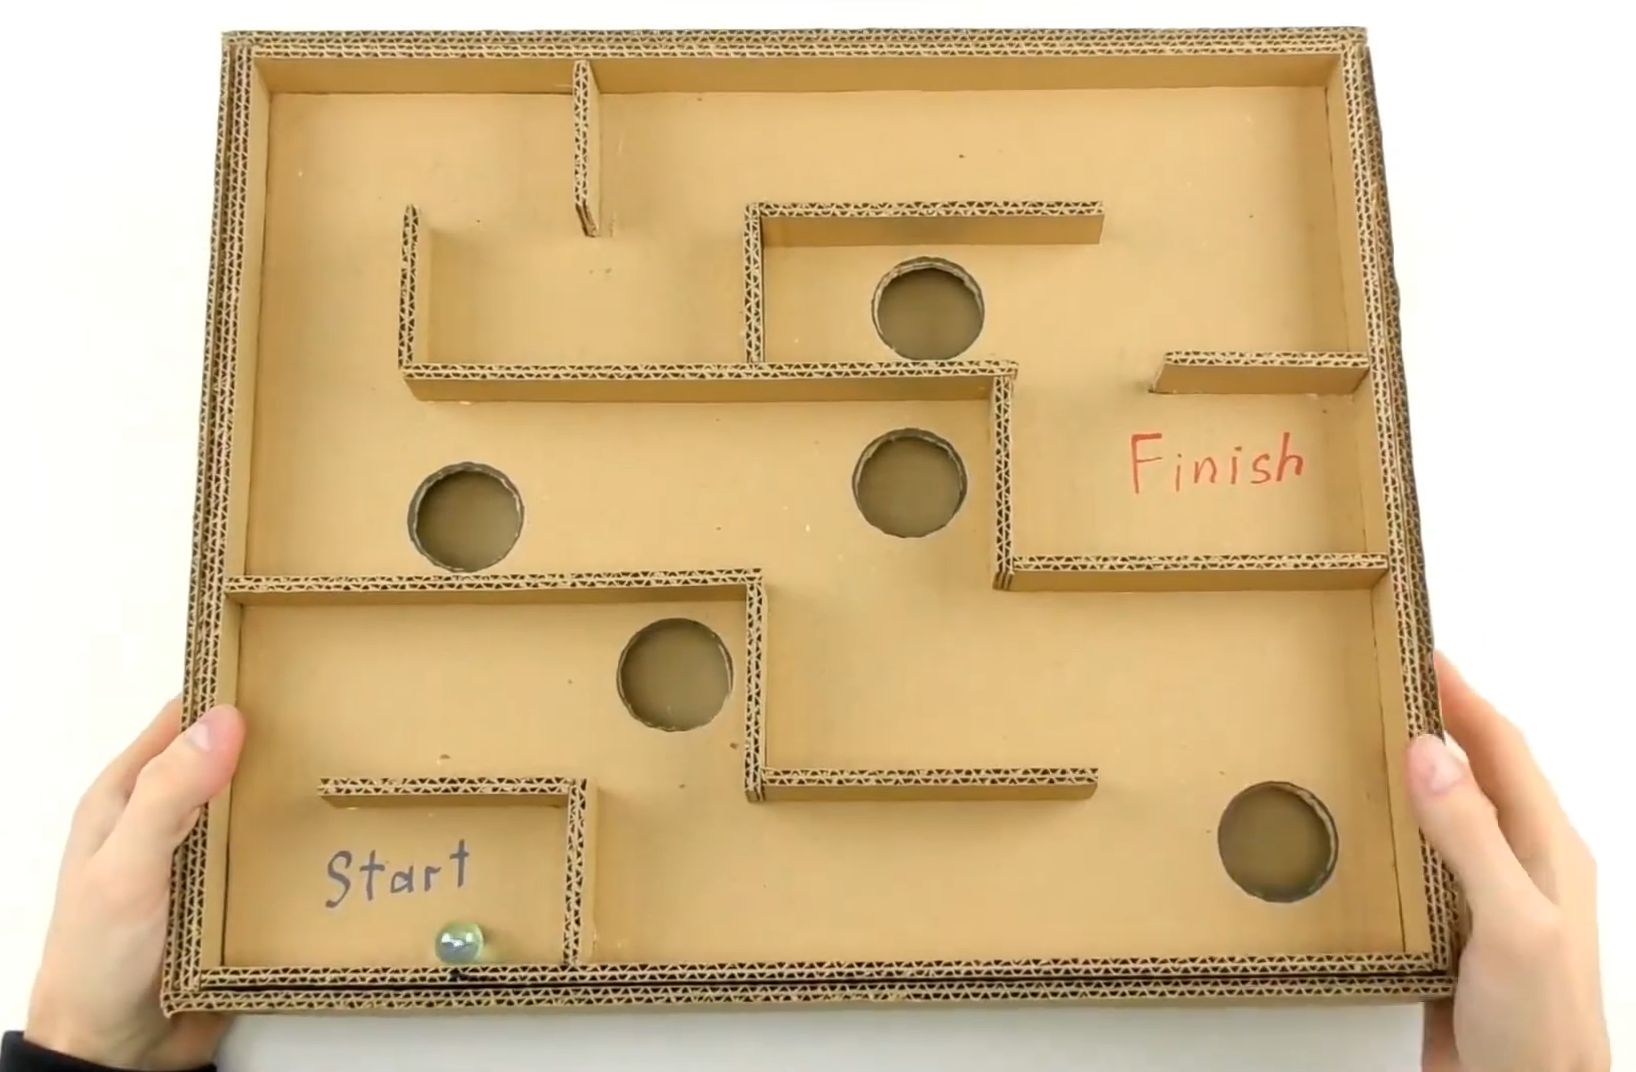
\includegraphics[width= 0.8\linewidth]{21}
		\vspace*{-10pt}
	\end{figure}
	Nếu chẳng may viên bi bị rơi xuống lỗ thì các em có thể lấy lại viên bi đó thông qua ô vuông ở trên hộp đã được tạo ra ở bước $4$.
	\begin{figure}[H]
		\vspace*{-5pt}
		\centering
		\captionsetup{labelformat= empty, justification=centering}
		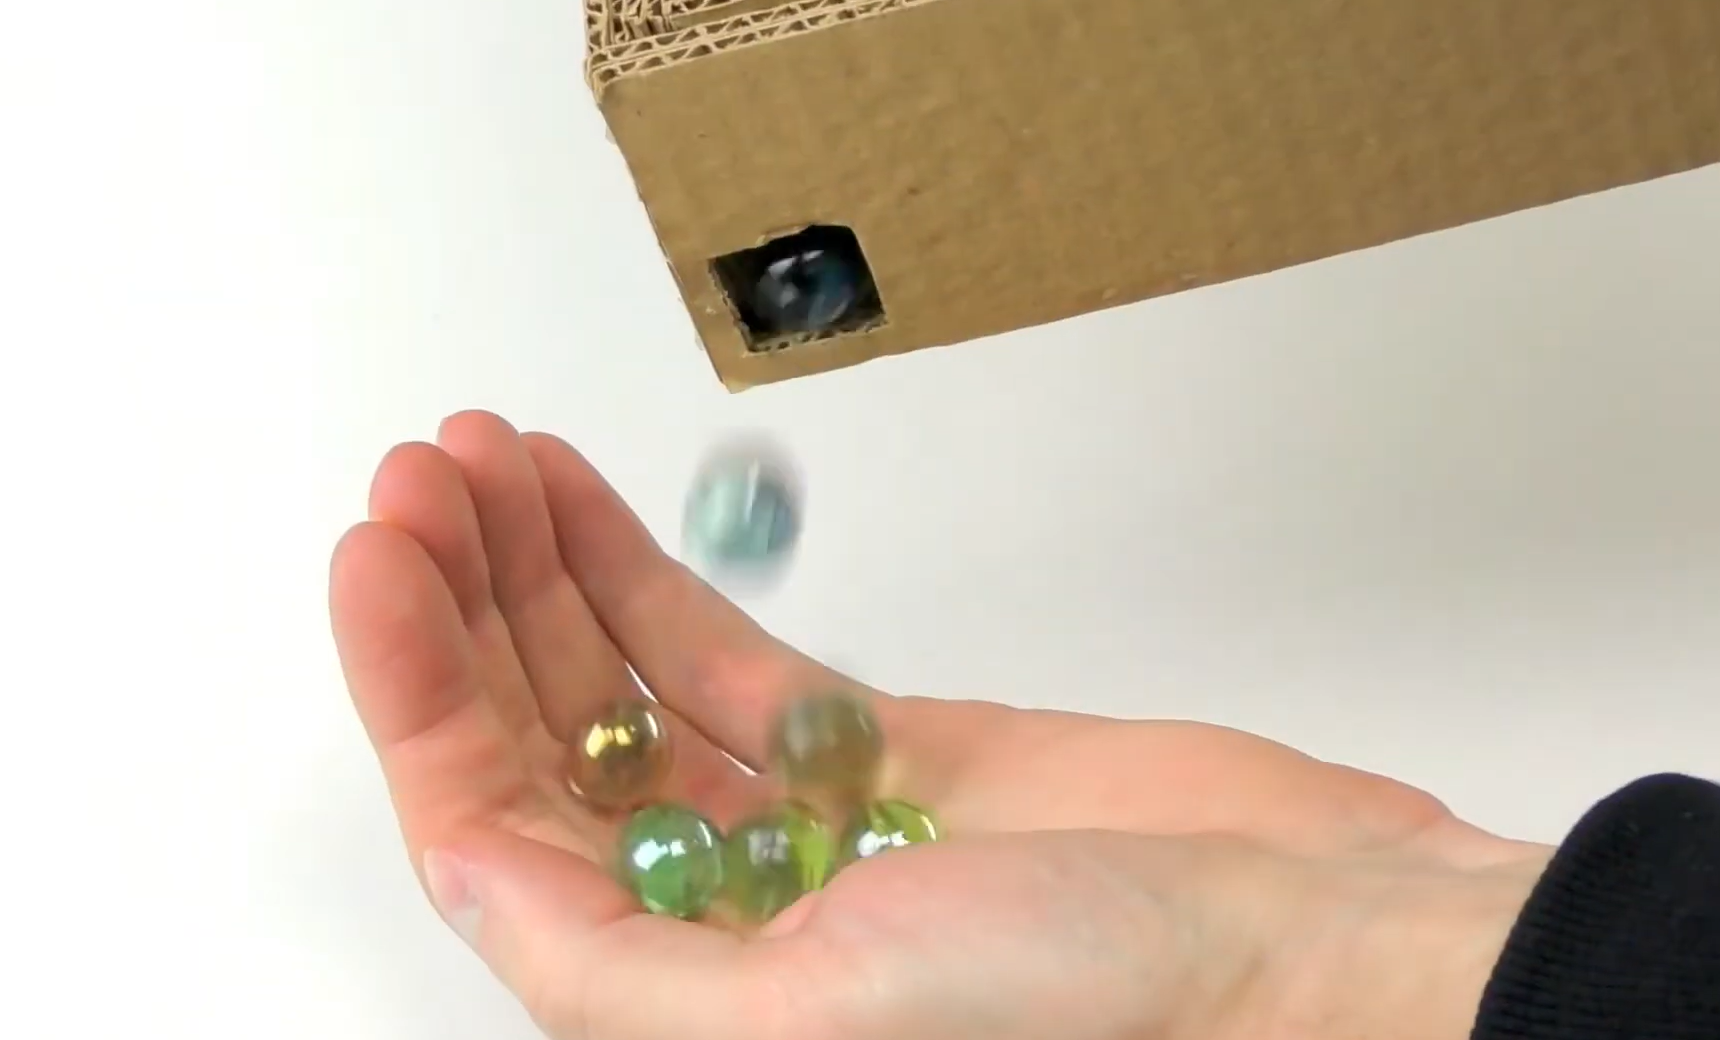
\includegraphics[width= 0.8\linewidth]{22}
		\vspace*{-10pt}
	\end{figure}
	\textbf{\color{toancuabi}Tài liệu tham khảo}
	\vskip 0.1cm
	\url{https://www.youtube.com/watch?v=5KN-foyuQa0&ab_channel=CityLofi}
\end{multicols}
%\newpage
%\graphicspath{{../toancuabi/pic/}}
%\begingroup
%\AddToShipoutPicture*{\put(122,680){
\includegraphics[scale=1]{../tieude.pdf}}}  
%\centering
%\endgroup
%\vspace*{25pt} 
%\begin{multicols}{2}
%	Thám tử Xuân Phong phải cải trang thành một nhà báo để tìm hiểu về một công ty nước giải khát có uy tín, tuy nhiên mới đây đã bất ngờ bị lộ bí mật về công thức pha chế với đối thủ cạnh tranh. Trong vai trò của một nhà báo, Xuân Phong tham gia một buổi họp đặc biệt gồm $n$ nhân viên chủ chốt của công ty. Xuân Phong được biết rằng, trong số $n$ người này có một người, có bí danh là Z, biết toàn bộ mọi nhân viên còn lại, tuy nhiên không một ai trong số $n-1$ người còn lại lại biết anh ta. Người có bí danh Z này có thể cho Xuân Phong đầu mối vì sao công thức pha chế bị lộ ra ngoài.
%	\vskip 0.1cm
%	Xuân Phong có thể tới cạnh mỗi một người bất kỳ trong buổi họp, và hỏi anh ta câu hỏi sau: ``Anh có biết <một người nào đó> không?" (trong ngoặc < > là một người cụ thể nào đó trong số những người còn lại). Rất may, khác với mọi lần, lần này  tất cả $n$ người đều nói thật, và Xuân Phong có thể hỏi một người nhiều hơn một lần.
%	\vskip 0.1cm
%	$a)$ Hỏi Xuân Phong có thể xác định được ai là Z sau khi đưa ra ít hơn $n$ câu hỏi được hay không?
%	\vskip 0.1cm
%	$b)$ Tìm số câu hỏi ít nhất đủ để Xuân Phong luôn tìm được nhân viên Z. Em hãy chứng minh rằng không thể hỏi ít hơn số câu hỏi như vậy được.
%	
%	\begin{figure}[H]
%		\centering
%		\vspace*{-5pt}
%		\captionsetup{labelformat= empty, justification=centering}
%		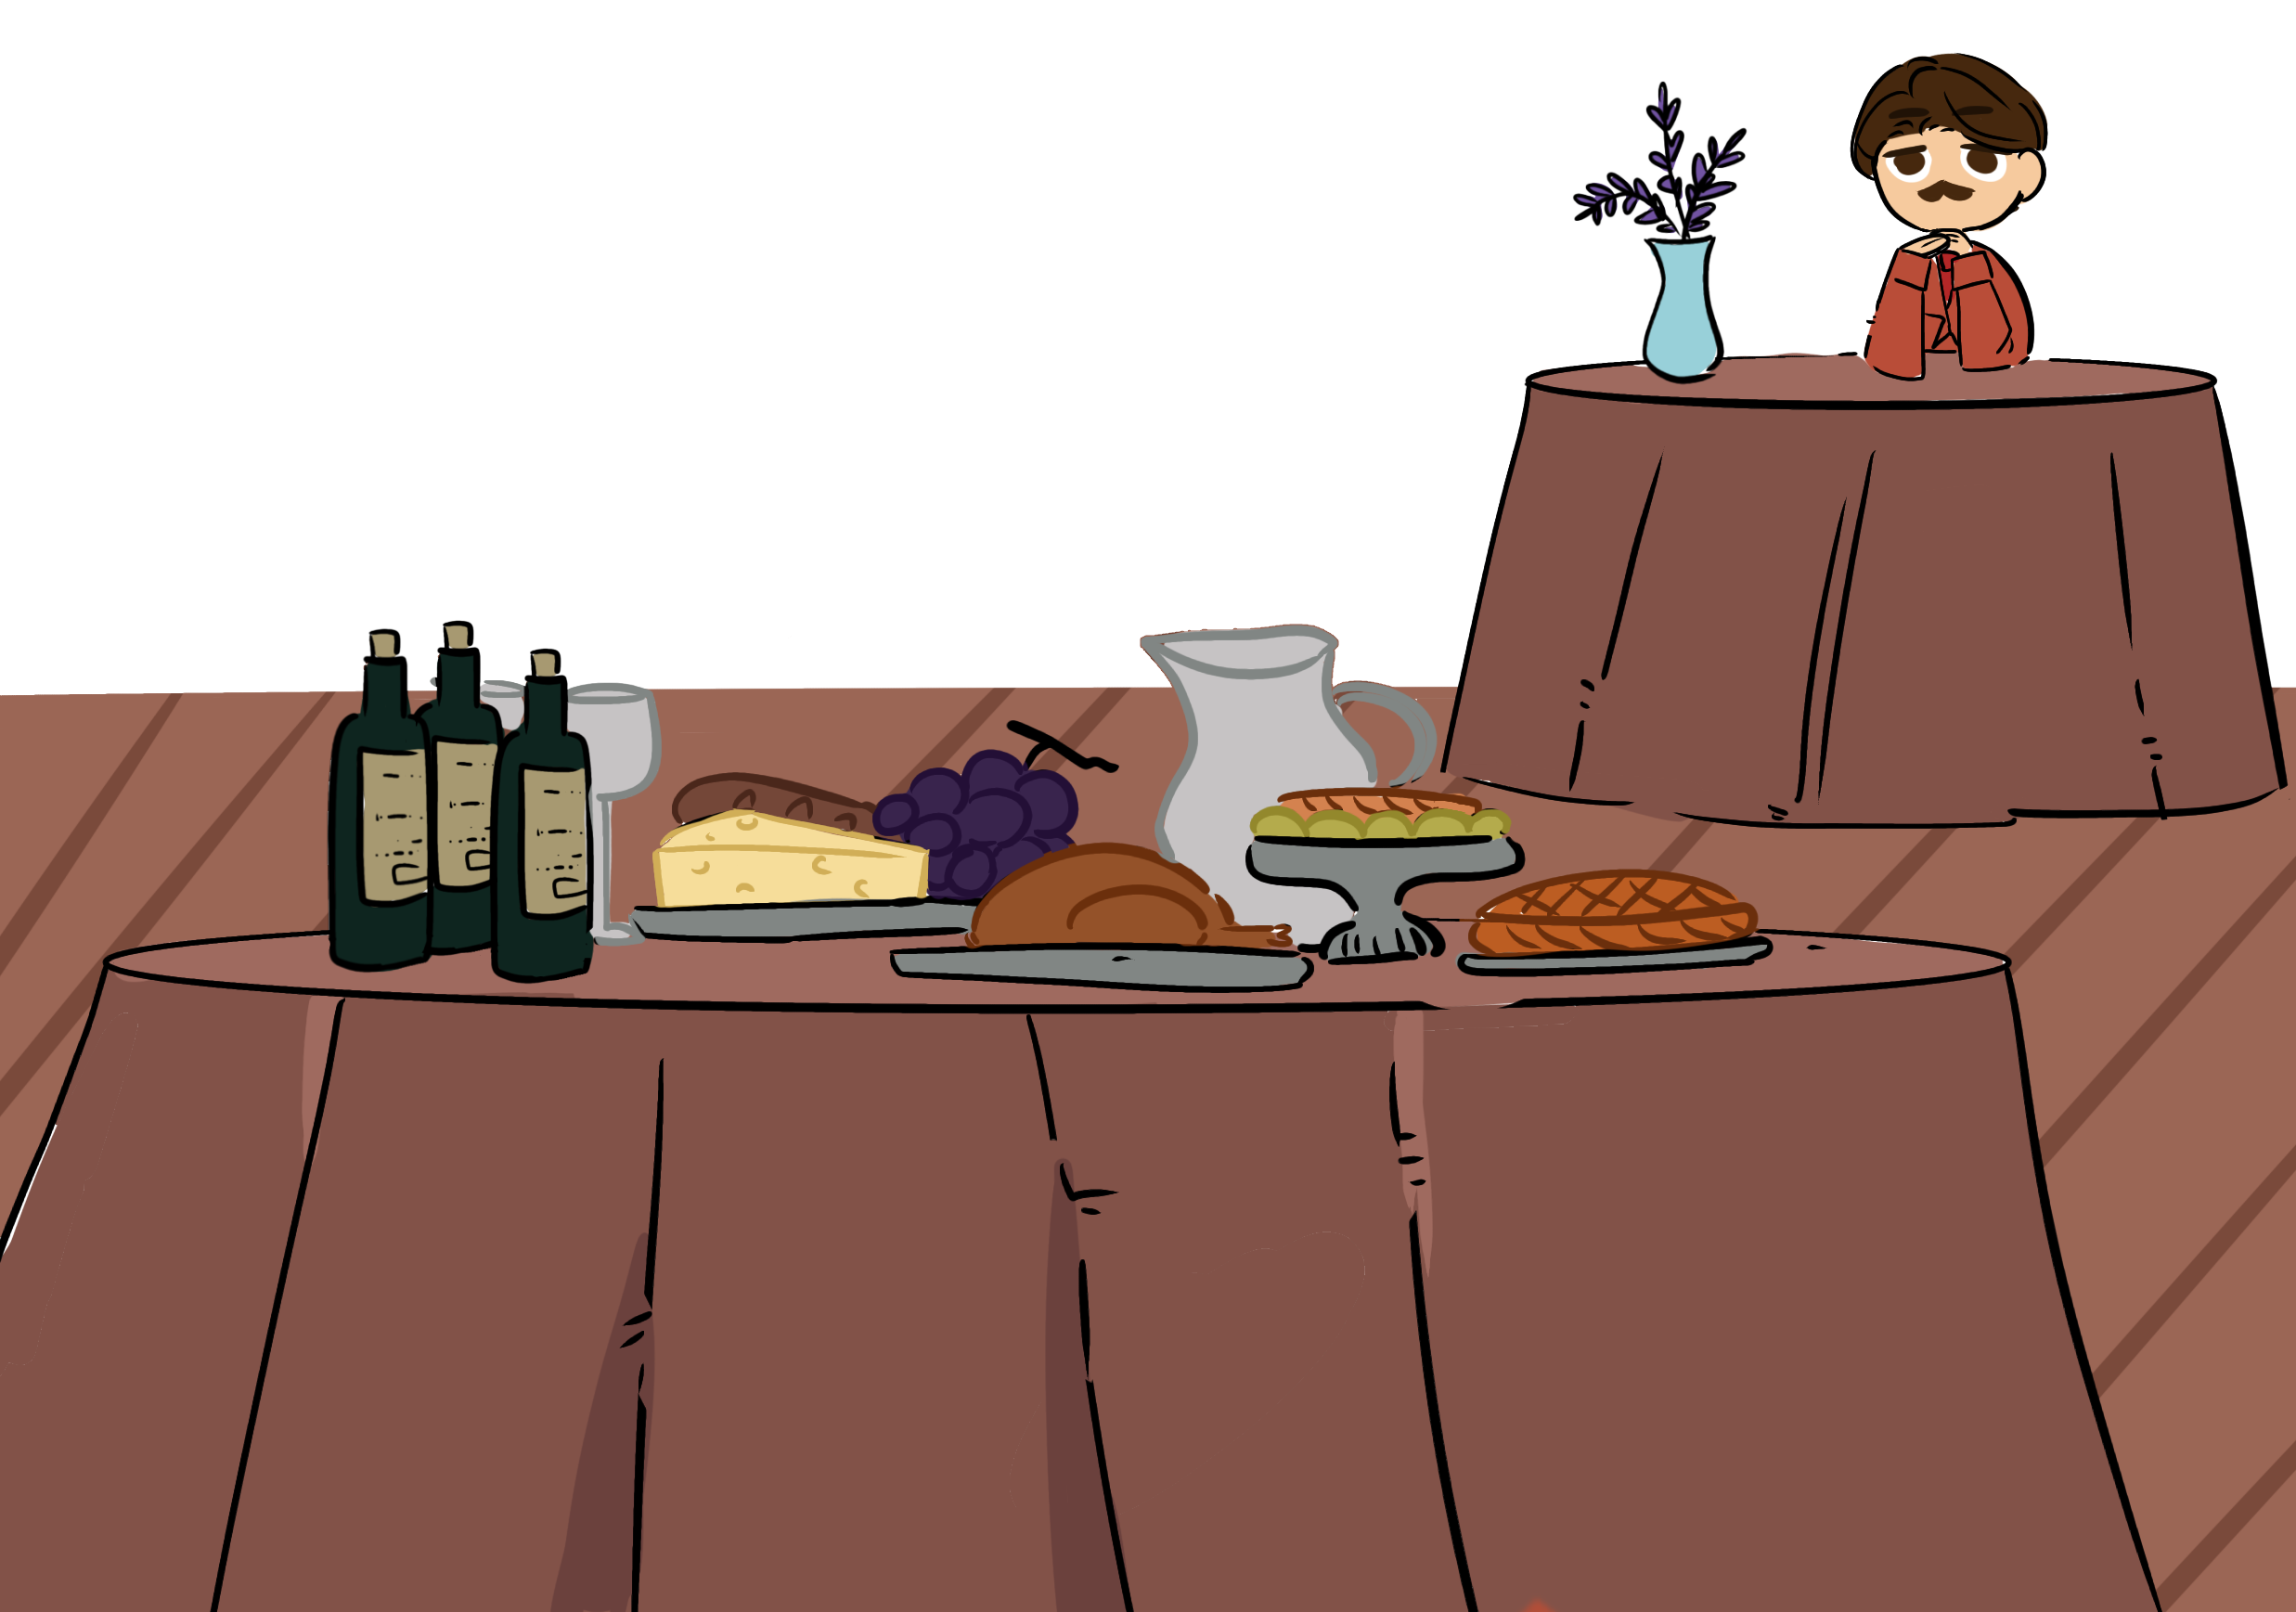
\includegraphics[width=1\linewidth]{xp}
%		\vspace*{-15pt}
%	\end{figure}
%\end{multicols}
%\newpage
%\begingroup
%\AddToShipoutPicture*{\put(120,670){
\includegraphics[scale=1]{../tieude11.pdf}}} 
%\centering
%\endgroup
%\vspace*{35pt}
%
%\begin{multicols}{2}
%	$\pmb{1.}$ Nàng Lọ Lem đi lạc vào trong rừng. Theo lời khuyên của bà tiên, nàng tìm thấy ba chiếc rương đựng những hạt dẻ có thể đem lại điều ước. Chiếc rương thứ nhất có ít hơn $6$ hạt dẻ so với  tổng số hạt dẻ ở hai chiếc rương còn lại. Chiếc rương thứ hai có ít hơn $10$ hạt dẻ so với tổng số hạt dẻ ở chiếc rương thứ nhất và thứ ba. Hỏi trong chiếc rương thứ ba có bao nhiêu hạt dẻ?
%	\begin{figure}[H]
%		\centering
%		\vspace*{-5pt}
%		\captionsetup{labelformat= empty, justification=centering}
%		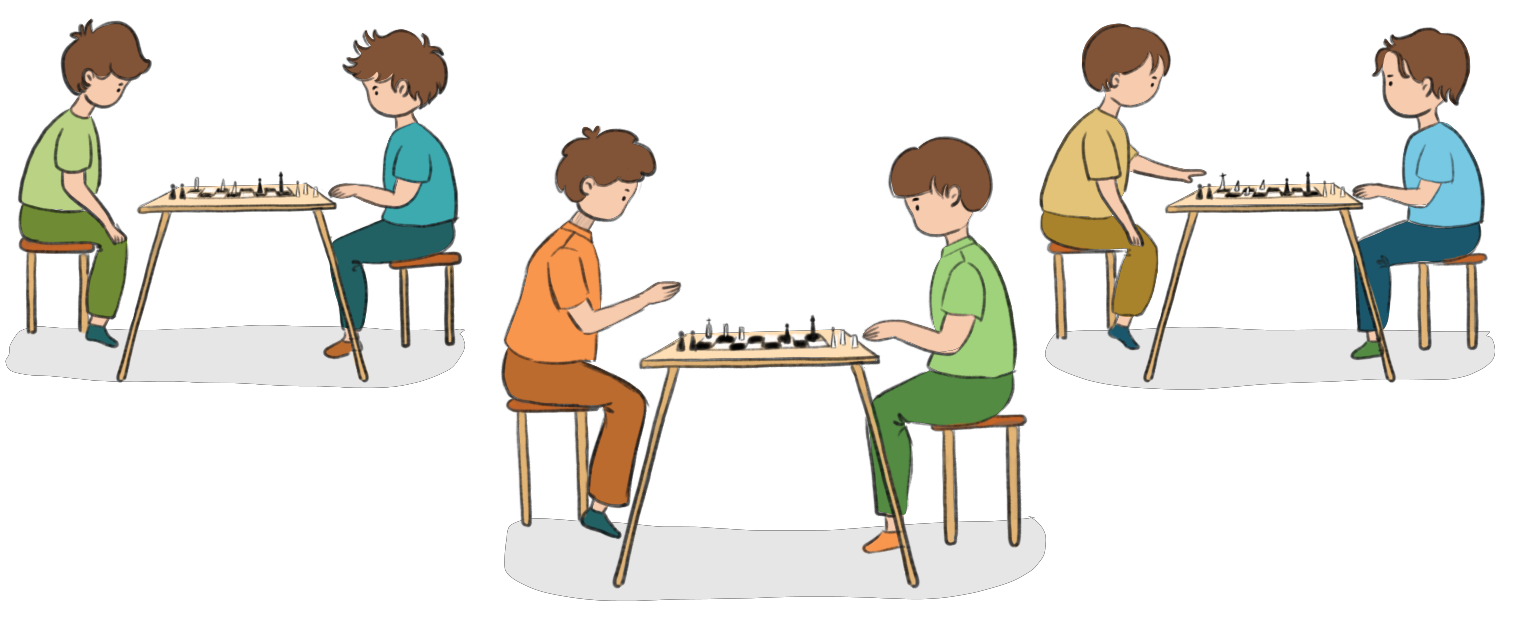
\includegraphics[width=0.85\linewidth]{Hinh1}
%		\vspace*{-10pt}
%	\end{figure}
%	$\pmb{2.}$ Bạn Vân viết $150$ chữ số xung quanh một vòng tròn. Nếu đọc $150$ chữ số này theo chiều kim đồng hồ bắt đầu từ một chỗ nào đó bất kì, thì Vân thấy số nhận được chia hết cho $27$. Em hãy chứng minh rằng, nếu Vân bắt đầu từ bất kỳ một chỗ khác và đọc ngược chiều kim đồng hồ toàn bộ $150$ chữ số đã viết, thì bạn cũng nhận được một số chia hết cho $27$.
%	\begin{figure}[H]
%		\centering
%		\vspace*{-5pt}
%		\captionsetup{labelformat= empty, justification=centering}
%		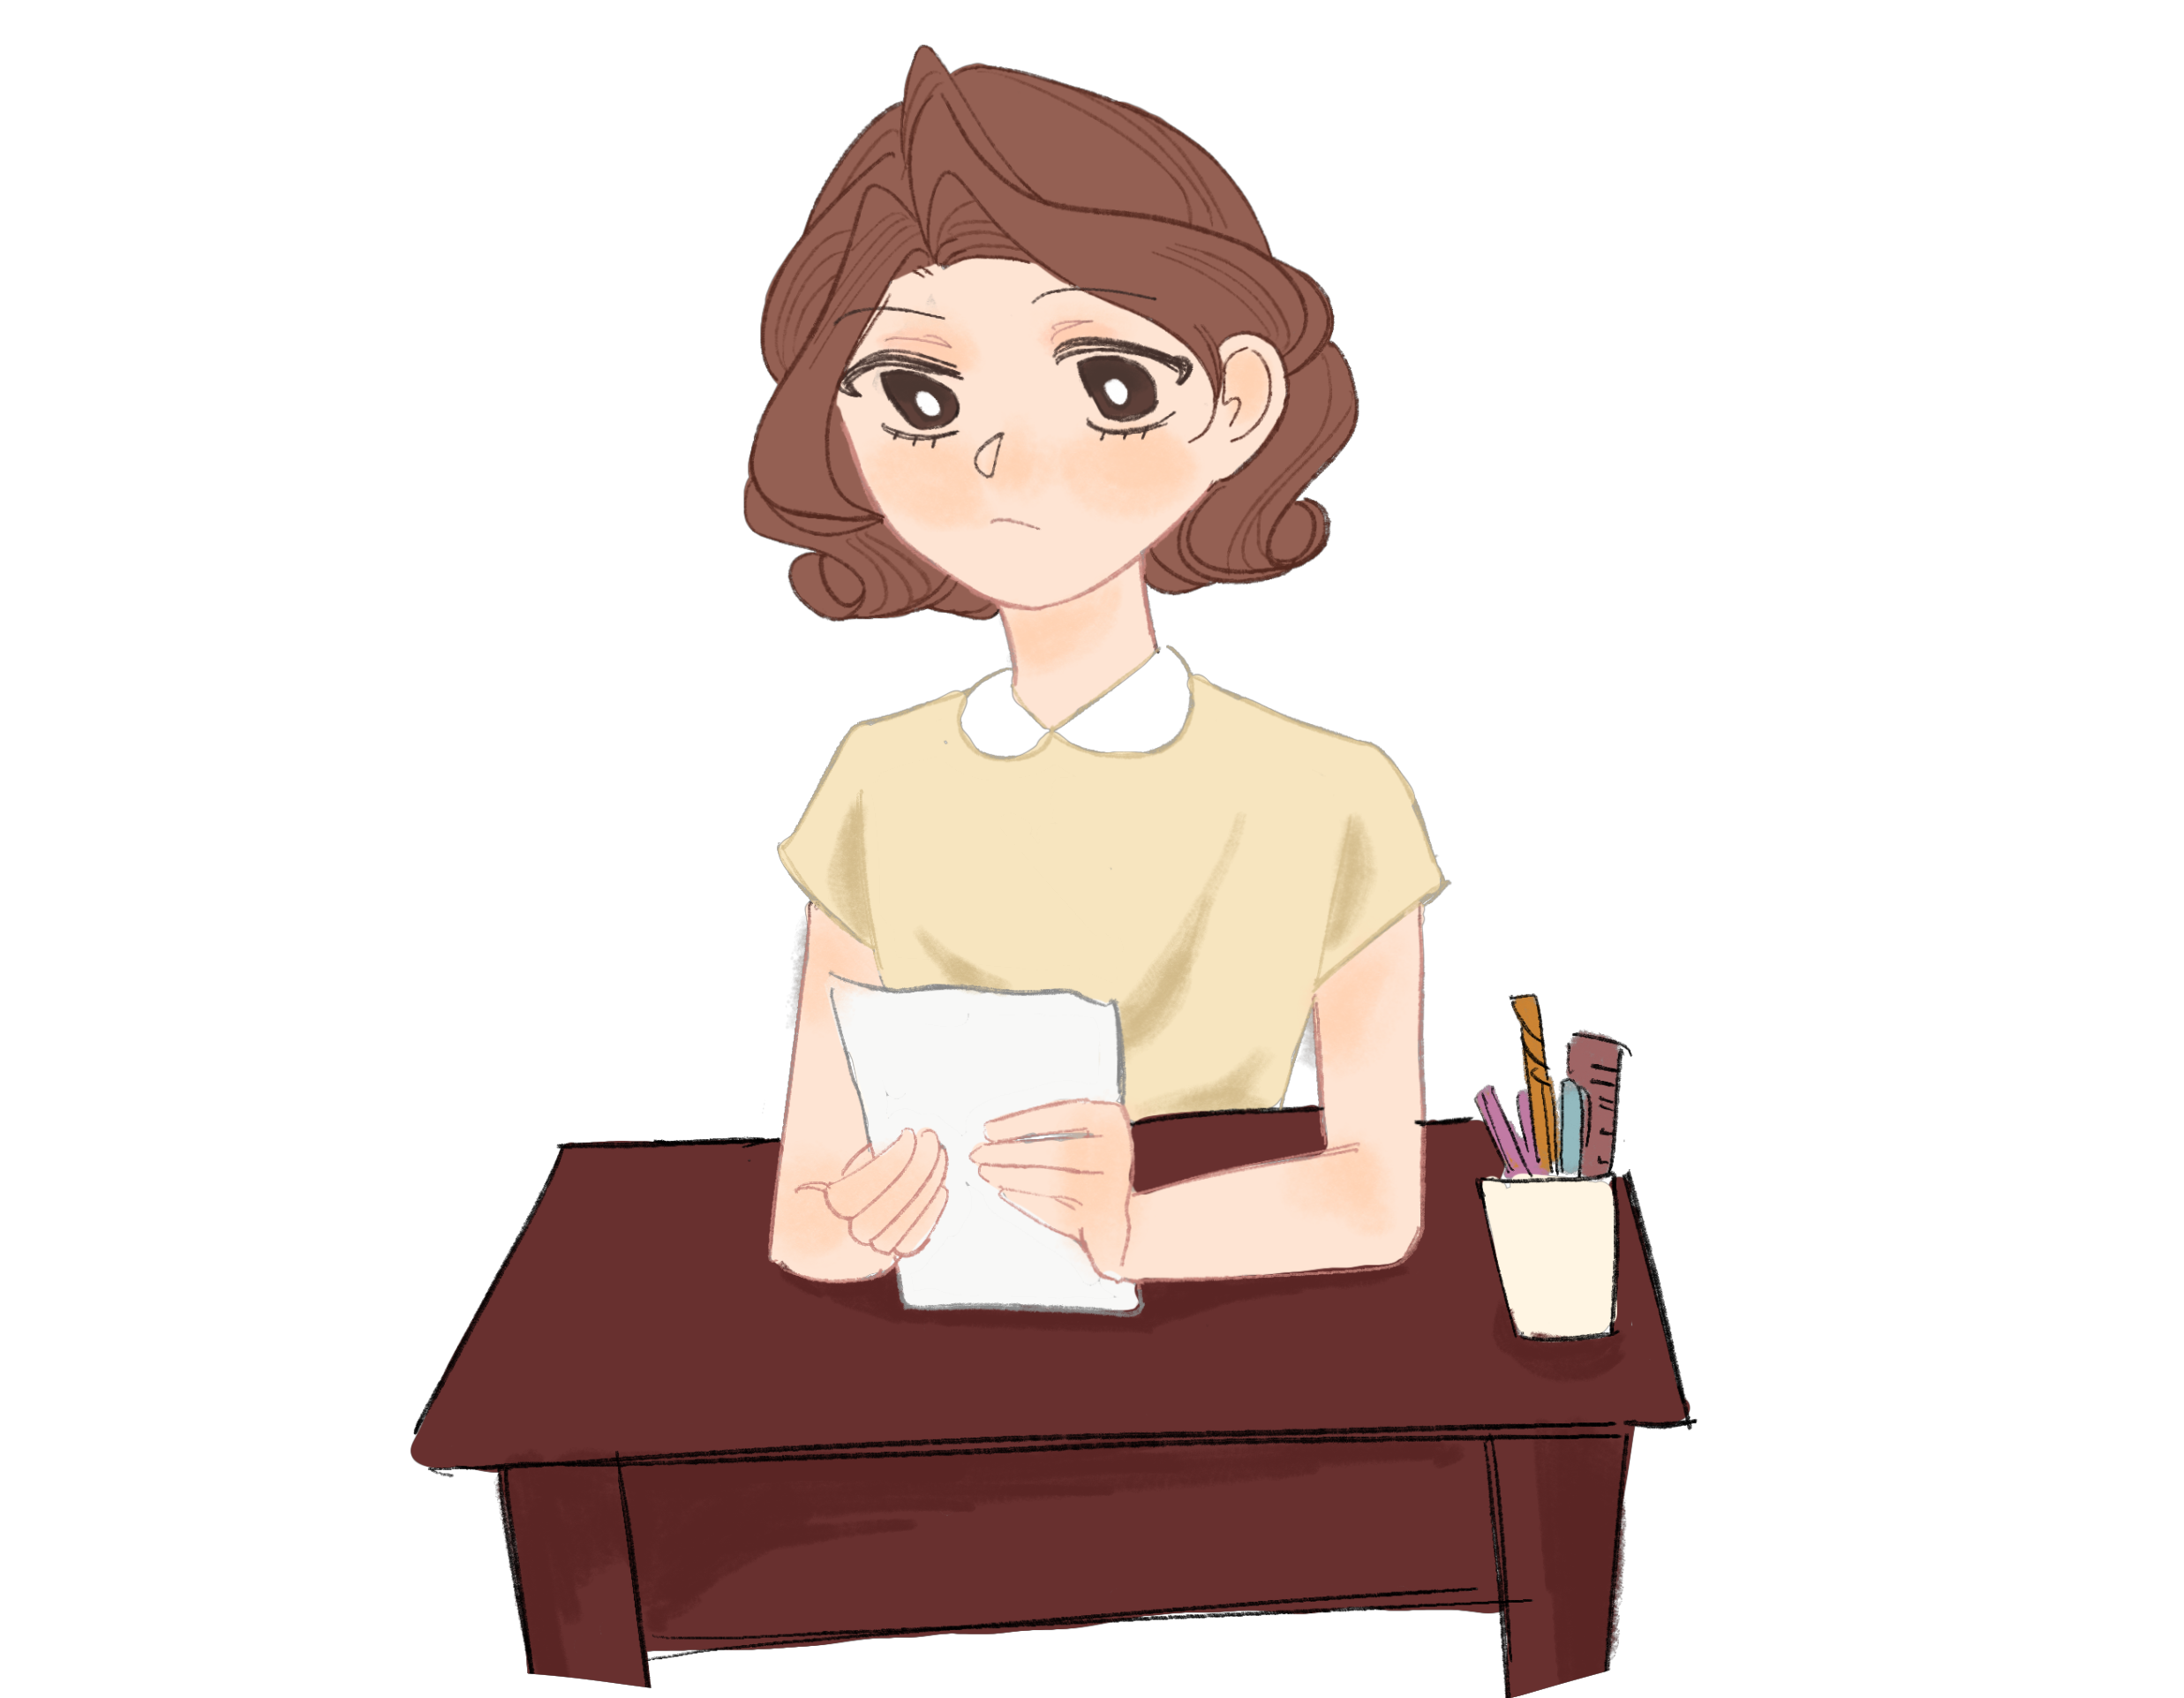
\includegraphics[width=0.85\linewidth]{Hinh2}
%		\vspace*{-5pt}
%	\end{figure}
%	$\pmb{3.}$ Có ba tên cướp ăn trộm được $10$ viên kim cương trong một két sắt với tổng giá trị là $4 000 000$ dollar. Chúng dự định sẽ phân chia những viên kim cương này cho nhau để mỗi tên có được ít nhất $1 000 000$ dollar. Khi bị cảnh sát truy đuổi, một viên kim cương trị giá $600 000$ dollar bị rơi mất, và vì thế chúng không thể chia được những viên kim cương như dự định ban đầu. Hỏi ba tên cướp này có bị nhầm lẫn ở đâu không, hay là trước khi bị rơi viên kim cương, việc chia đồ ăn trộm của chúng đã không thể thực hiện được theo như dự định?
%	\begin{figure}[H]
%		\centering
%		\vspace*{-5pt}
%		\captionsetup{labelformat= empty, justification=centering}
%		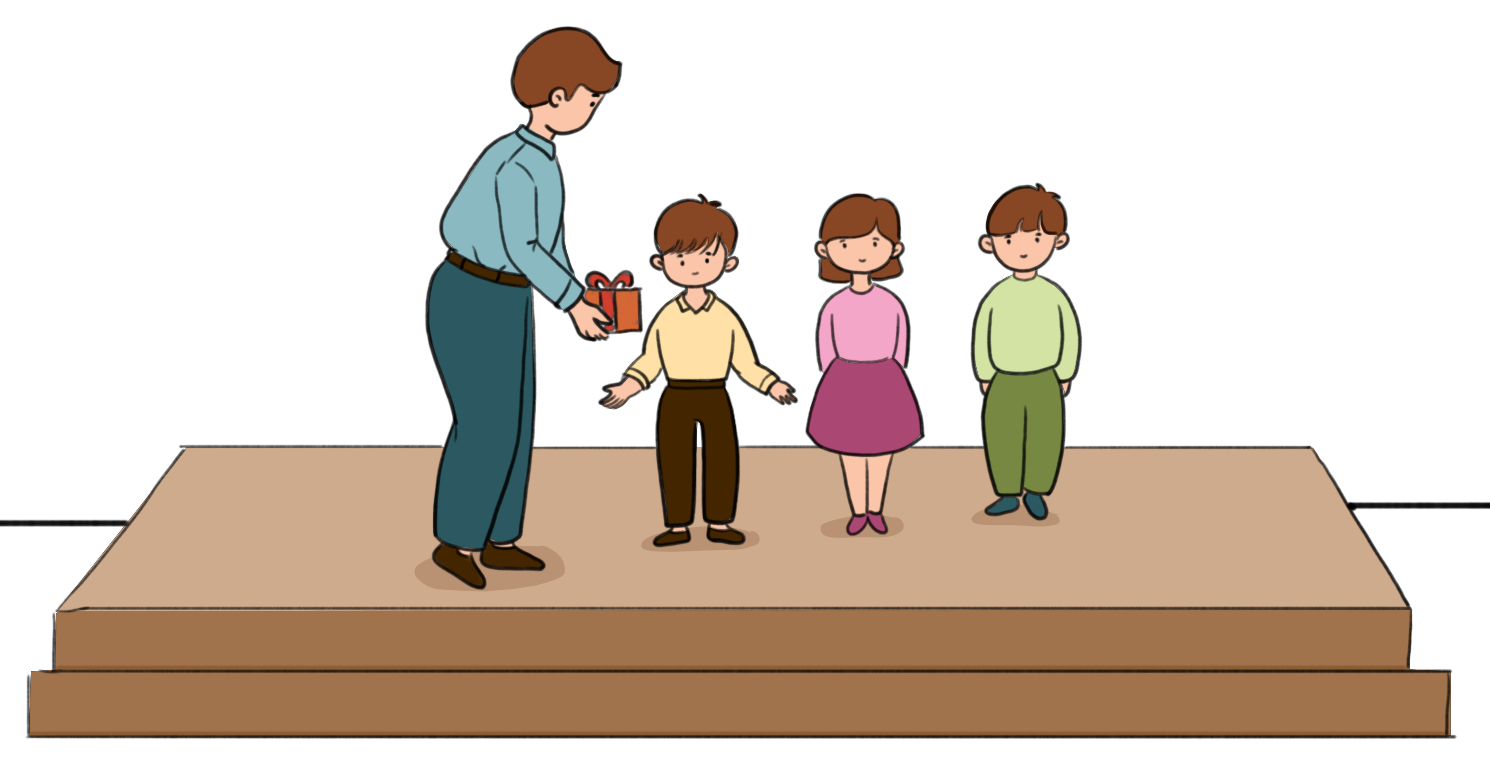
\includegraphics[width=1\linewidth]{Hinh3}
%		\vspace*{-15pt}
%	\end{figure}
%	$\pmb{4.}$ 	Bác Tâm mua một bao tải gạo nặng $9$ kg. Bác muốn chia ra thành hai túi nhỏ hơn, một túi nặng $2$ kg, còn túi kia nặng $7$ kg. Bác chỉ có một bàn cân đĩa thăng bằng với hai quả cân, một quả nặng $50$ g, còn quả kia nặng $200$ g. Em hãy giúp bác Tâm thực hiện phép san gạo ra hai túi nhỏ như trên chỉ tối đa sau ba lần cân.
%	\begin{figure}[H]
%		\centering
%%		\vspace*{-5pt}
%		\captionsetup{labelformat= empty, justification=centering}
%		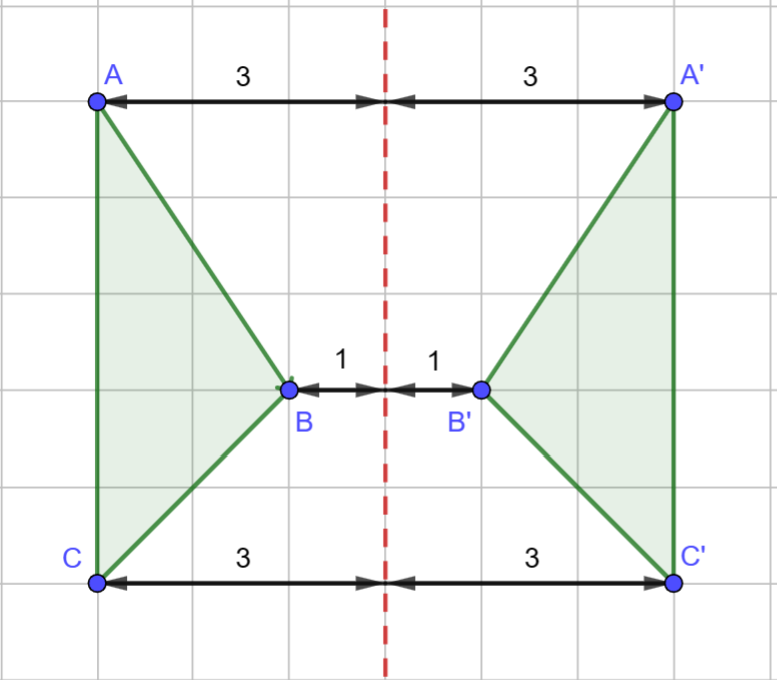
\includegraphics[width=1\linewidth]{Hinh4}
%		\vspace*{-10pt}
%	\end{figure}
%	\vskip 0.1cm
%	$\pmb{5.}$ 	Có $6$ đồng xu hình thức bên ngoài giống hệt nhau. Bốn đồng xu trong số đó là thật, mỗi đồng có khối lượng đúng $4$ g, còn hai đồng xu là giả có tổng khối lượng là $8$ g nhưng có một đồng nặng hơn một chút, còn một đồng nhẹ hơn một chút. Hỏi có thể sử dụng một bàn cân thăng bằng (không có quả cân) để sau tối đa bốn lần cân phát hiện được hai đồng xu giả được hay không?
%	\begin{figure}[H]
%		\centering
%		\vspace*{-5pt}
%		\captionsetup{labelformat= empty, justification=centering}
%		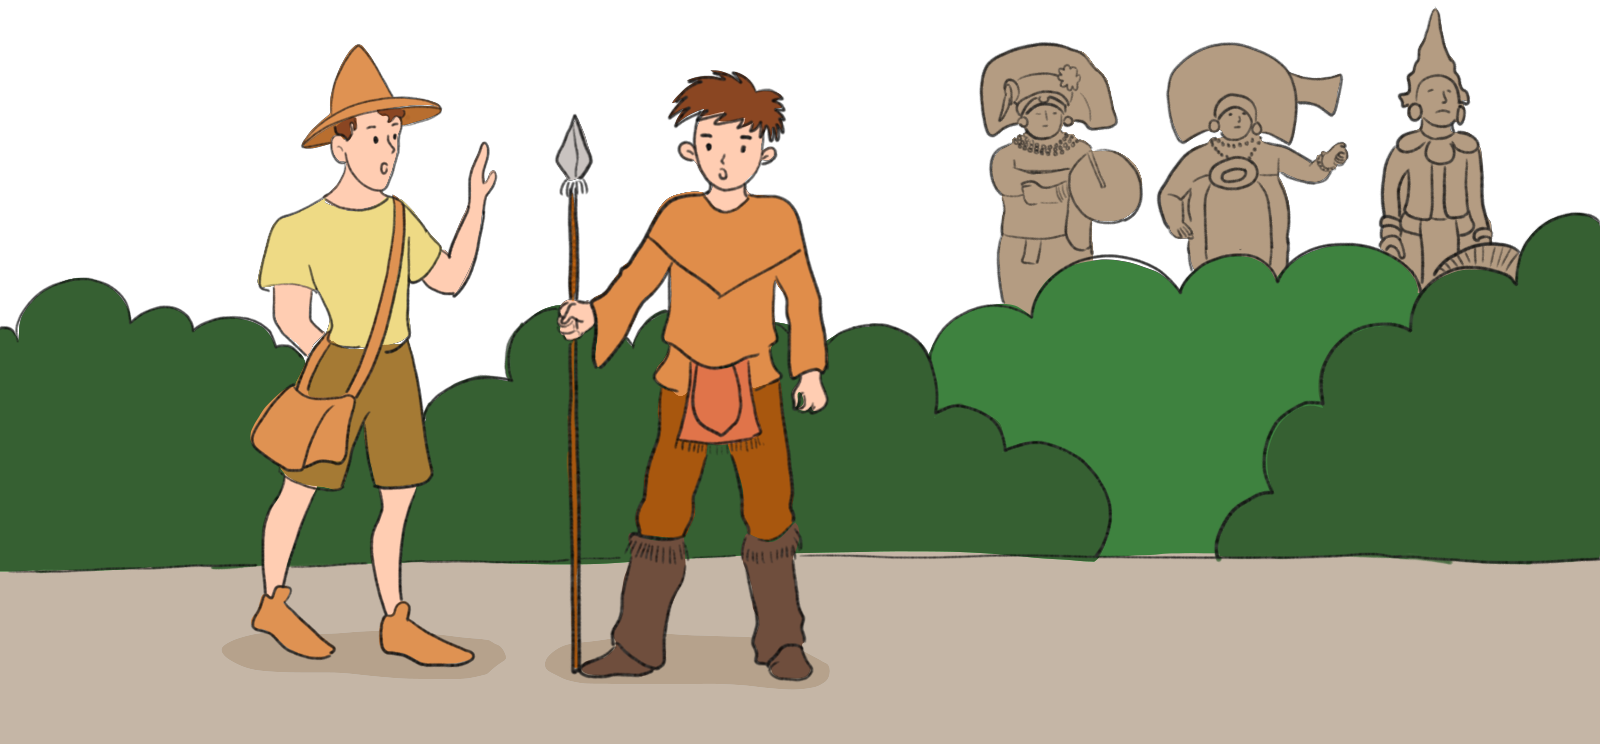
\includegraphics[width=1\linewidth]{Hinh5}
%		\vspace*{-20pt}
%	\end{figure}
%	$\pmb{6.}$ 	Trong một giải vô địch đá bóng của trường, đội dành huy chương vàng có được tổng số điểm là $7$, đội dành huy chương bạc có tổng số điểm là $5$, còn đội dành huy chương đồng có tổng số điểm là $3$. Biết rằng trong giải đấu này các đội thi đấu theo hình thức vòng tròn $1$ lượt, mỗi đội thi đấu với một đội khác đúng một trận, và trong mỗi trận mỗi đội sẽ nhận được $2$ điểm nếu thắng, $1$ điểm nếu hoà, $0$ điểm nếu thua. Nếu hai đội có cùng tổng số điểm thì vị trí thứ tự sẽ được xác định bằng hiệu số bàn thắng và bàn thua. Hỏi 
%	\vskip 0.1cm
%	$a)$ Đội đứng ở vị trí thấp nhất có được tổng số điểm là bao nhiêu?
%	\vskip 0.1cm
%	$b)$	Có bao nhiêu đội tham gia giải vô địch.
%	\begin{figure}[H]
%		\centering
%		\vspace*{-10pt}
%		\captionsetup{labelformat= empty, justification=centering}
%		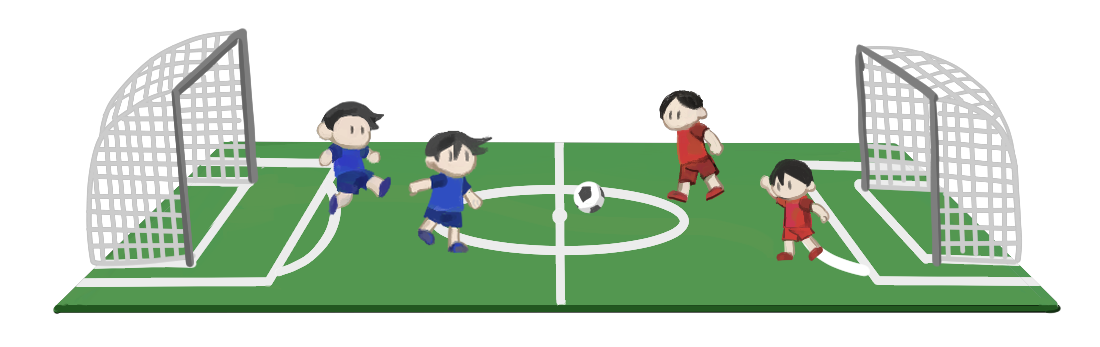
\includegraphics[width=1\linewidth]{Hinh6}
%		\vspace*{-10pt}
%	\end{figure}
%\end{multicols}
%\vspace*{-10pt}
%{\color{toancuabi}\rule{1\linewidth}{0.1pt}}
%\begingroup
%\AddToShipoutPicture*{\put(116,342){
\includegraphics[scale=1]{../tieude2.pdf}}} 
%\centering
%\endgroup
%\vspace*{75pt}
%
%\begin{multicols}{2}
%	$\pmb{1.}$ 	Tại thành phố Hoa Hướng Dương, trong số các cậu bé tí hon có $5$ cậu ngày nào cũng ăn bánh rán ngọt, có $7$ cậu bé cứ cách một ngày lại ăn bánh rán ngọt, còn tất cả các cậu bé tí hon còn lại không bao giờ ăn bánh rán ngọt. Ngày hôm qua có $9$ cậu bé tí hon đã ăn bánh rán ngọt. Hỏi trong ngày hôm nay sẽ có bao nhiêu cậu bé tí hon ăn bánh rán ngọt?
%	\begin{figure}[H]
%		\centering
%		\vspace*{-5pt}
%		\captionsetup{labelformat= empty, justification=centering}
%		\includegraphics[width=1\linewidth]{Pi9_bai1}
%		\vspace*{-15pt}
%	\end{figure}
%	\textit{Lời giải.} 	Trong số $9$ cậu bé tí hon ăn bánh rán ngọt ngày hôm qua có $5$ cậu ăn bánh rán mỗi ngày, như vậy $4$ cậu còn lại ăn bánh rán cách $1$ ngày. Do đó trong ngày hôm nay $4$ cậu này sẽ không ăn bánh rán, còn những cậu bé còn lại (có $3$ cậu) trong số các cậu ăn bánh cách $1$ ngày lại sẽ ăn bánh. Vì thế $3$ cậu này sẽ ăn bánh trong ngày hôm nay, cùng với cả $5$ cậu ăn bánh rán mỗi ngày. Ta có đáp số là: $3+5 = 8$ (cậu bé tí hon).
%	\vskip 0.1cm
%	$\pmb{2.}$ Một cửa hàng bán hoa tươi có ba loại hoa hồng: hồng tím, hồng vàng và hồng đỏ. Số hoa hồng tím bằng một nửa tổng số hoa hồng vàng và hồng đỏ. Số hoa hồng đỏ lại bằng một phần ba tổng số hoa hồng vàng và số hoa hồng tím. Biết rằng số hoa hồng vàng là $45$ bông. Hỏi cửa hàng có bao nhiêu hoa hồng tím và hoa hồng đỏ?
%	\vskip 0.1cm
%	\textit{Lời giải.} 	Số hoa hồng tím bằng một nửa tổng số hoa hồng vàng và hồng đỏ, có nghĩa là số hoa hồng tím bằng $1/3$ tổng số hoa hồng. Tương tự, số hoa hồng đỏ chiếm $1/4$ tổng số hoa hồng. Ta có thể vẽ sơ đồ đoạn thẳng, có độ dài bằng $12$ đoạn nhỏ (cho thuận tiện việc biểu diễn $1/3$ và $1/4$ tổng số). Số hoa hồng tím tương ứng $4$ đoạn nhỏ, còn số hoa hồng đỏ tương ứng $3$ đoạn. Suy ra số hoa hồng vàng tương ứng với $12 - 3 - 4 = 5$ (đoạn). Như vậy mỗi đoạn nhỏ tương ứng với $45/5 = 9$ (bông hoa). Do đó, số hoa hồng tím là $4\times 9=36$ (bông) và số hoa hồng đỏ là $3\times 9=27$ (bông).
%	\begin{figure}[H]
%		\centering
%		\vspace*{-5pt}
%		\captionsetup{labelformat= empty, justification=centering}
%		\includegraphics[width=1\linewidth]{Pi9_bai2}
%		\vspace*{-15pt}
%	\end{figure}
%	$\pmb{3.}$ Thỏ Hồng đi đón $3$ cậu bạn của mình là Ngựa Đốm, Ngựa Bạch và Gấu Nâu lặn lội đến thăm nhà mình. Vừa ra tới bìa rừng, Thỏ Hồng đã thấy lờ mờ ba bạn đứng hàng ngang ở xa xa ngoài bãi cỏ, nhưng vì sương mù dày đặc, Thỏ Hồng không thể nhận ra ai với ai. Thỏ Hồng bèn kêu các bạn tự giới thiệu để biết được từng vị khách. Cậu bạn đứng ở ngoài cùng bên trái từ vị trí quan sát của Thỏ Hồng nói rằng: ``Có Gấu Nâu đứng cạnh tôi đấy". Cậu bạn đứng ở ngoài cùng bên tay phải, lại tuyên bố rằng: ``Đó là Ngựa Bạch vừa nói với cậu đấy". Cuối cùng, cậu bạn đứng ở giữa, thông báo rằng: ``Bên tay trái của tôi là Ngựa Đốm đấy". Các em hãy tìm ra bạn nào đứng ở đâu trong số $3$ người bạn của Thỏ Hồng, biết rằng Ngựa Đốm thì chuyên nói dối, Ngựa Bạch thì thỉnh thoảng nói dối, còn Gấu Nâu thì không bao giờ nói dối Thỏ Hồng.
%	\vskip 0.1cm
%	\textit{Lời giải.} Nếu như Gấu Nâu đứng ở ngoài cùng bên trái (từ vị trí quan sát của Thỏ Hồng), thì cậu bạn đứng giữa cũng phải là Gấu Nâu -- điều này là mâu thuẫn. Nếu như Gấu Nâu đứng ở giữa, thì bên tay phải (theo Thỏ Hồng quan sát) sẽ là Ngựa Đốm, còn bên ngoài cùng tay trái sẽ là Ngựa Bạch. Nhưng như vậy, Ngựa Đốm sẽ nói thật, ta lại suy ra mâu thuẫn.
%	\begin{figure}[H]
%		\centering
%		\vspace*{-5pt}
%		\captionsetup{labelformat= empty, justification=centering}
%		\includegraphics[width=1\linewidth]{Pi9_bai3}
%		\vspace*{-15pt}
%	\end{figure}
%	Cuối cùng, chỉ khi Gấu Nâu đứng ngoài cùng bên phải ta mới không gặp mâu thuẫn. Khi đó ngoài cùng tay trái là Ngựa Bạch, ở giữa là là Ngựa Đốm -- hai cậu bạn này đều nói dối.
%	\vskip 0.1cm
%	\textit{Đáp số}: Từ chỗ quan sát của Thỏ Hồng, ngoài cùng tay trái là Ngựa Bạch, ở giữa là Ngựa Đốm, còn đứng ngoài cùng bên phải là Gấu Nâu.
%	\vskip 0.1cm
%	$\pmb{4.}$ Có $7$ quả táo, khối lượng mỗi quả có thể khác nhau để ở trên bàn. Bạn Thanh nhận thấy rằng có thể đặt $3$ quả trên một đĩa cân và $4$ quả còn lại trên đĩa cân bên kia sao cho hai bên cân thăng bằng. Bạn Thịnh lại thấy rằng có thể đặt $2$ quả táo trên một đĩa cân, và $5$ quả còn lại trên đĩa cân bên kia và hai bên cân cũng thăng bằng. Em hãy chỉ ra rằng có thể đặt trên một đĩa cân bên này $1$ quả táo và đặt trên đĩa cân bên kia $3$ quả táo trong số $7$ quả đã cho, sao cho hai bên cân cũng vẫn thăng bằng.
%	\begin{figure}[H]
%		\centering
%		\vspace*{-5pt}
%		\captionsetup{labelformat= empty, justification=centering}
%		\includegraphics[width=1\linewidth]{Pi9_bai4}
%		\vspace*{-15pt}
%	\end{figure}
%	\textit{Lời giải.} 	Để dễ dàng hình dung, ta có thể giả sử rằng Thanh đặt được $3$ quả táo đỏ ở đĩa cân bên trái và $4$ quả táo xanh ở đĩa cân bên phải để cân thăng bằng. Vì vậy nếu Thịnh đặt bất kỳ hai quả táo cùng màu ở một bên và $5$ quả còn lại ở đĩa bên kia thì $5$ quả này sẽ luôn nặng hơn (điều này cũng tương đương với việc có những quả táo nào đó sau lần cân thăng bằng của Thanh đã bị chuyển sang đĩa cân bên kia).
%	\vskip 0.1cm
%	Vì vậy để cho cân thăng bằng, Thịnh chỉ có thể đặt hai quả táo khác màu trên một đĩa cân, và $5$ quả còn lại sang đĩa bên kia. Nhưng điều này cũng tương đương với việc sau khi Thanh đã cân được thăng bằng, Thịnh đã đổi chỗ $2$ quả táo đỏ với $1$ quả táo xanh. Nếu như bỏ $3$ quả này đi, thì trên một đĩa cân có $1$ quả táo đỏ và trên đĩa bên kia có $3$ quả táo xanh, và hơn nữa cân hai bên vẫn thăng bằng.
%	\vskip 0.1cm
%	Các em có thể làm bài này bằng lập luận theo dạng của biểu thức đại số, lập ra hai phương trình và tìm hiệu của chúng.
%	\vskip 0.1cm
%	$\pmb{5.}$ Có $20$ chiếc túi nilon, mỗi túi đựng $26$ quả mận. Biết rằng tổng khối lượng của mỗi túi không vượt quá $1$ kg. Em hãy chỉ ra rằng có thể xếp số mận trên vào $26$ chiếc túi nilon, mỗi túi có đúng $20$ quả mận, sao cho tổng khối lượng của mỗi túi nhỏ hơn $1$ kg.
%	\begin{figure}[H]
%		\centering
%		\vspace*{-5pt}
%		\captionsetup{labelformat= empty, justification=centering}
%		\includegraphics[width=0.8\linewidth]{Pi9_bai5}
%		\vspace*{-5pt}
%	\end{figure}
%	\textit{Lời giải.} 	Ta nhặt ra từ mỗi túi ban đầu quả mận nhẹ nhất và xếp chúng vào chiếc túi thứ $21$. Do mỗi quả nhẹ nhất này có khối lượng không quá $\dfrac{1}{26}$ kg, nên tổng khối lượng của $20$ quả được nhặt ra này không quá $\dfrac{20}{26} <1$ (kg). Hơn nữa khối lượng của mỗi túi ban đầu giờ đều nhẹ hơn $1$ kg, và trong mỗi túi có đúng $25$ quả. Ta lại lặp lại quá trình trên: nhặt ra trong mỗi túi trong số $20$ túi ban đầu quả mận nhẹ nhất (tức là quả mận nhẹ thứ nhì, sau khi đã nhặt ra lần đầu tiên), và đưa $20$ quả này vào chiếc túi thứ $22$, khi đó tổng khối lượng mận ở chiếc túi thứ $22$ này sẽ nhỏ hơn $\dfrac{20}{25}$ (kg). Ta cứ làm như vậy, cho đến khi đạt đến chiếc túi thứ $26$ (sau $6$ lần nhặt ra).
%	\vskip 0.1cm
%	$\pmb{6.}$ 	Có $100$ số $1, 2, 3, \ldots, 100$ được viết ra thành hàng ngang từ trái qua phải theo thứ tự tăng dần. Bạn Long và bạn Lâm chơi một trò chơi như sau. Hai bạn lần lượt đến lượt chơi của mình sẽ đặt duy nhất một trong các dấu $+$, $-$ hoặc $\times$ vào vị trí bất kỳ xen kẽ giữa hai số trong $100$ số nói trên. Bạn đi lượt cuối cùng sẽ thắng nếu số nhận được bằng cách thực hiện phép tính bởi $100$ số và các phép tính đã điền giữa chúng là một số lẻ. Em hãy chỉ ra rằng nếu Long là người đi đầu tiên (và cũng sẽ là người đi cuối cùng) thì Long luôn có cách chơi để thắng.
%	\begin{figure}[H]
%		\centering
%		\vspace*{-5pt}
%		\captionsetup{labelformat= empty, justification=centering}
%		\includegraphics[width=0.7\linewidth]{Pi9_bai6}
%		\vspace*{-5pt}
%	\end{figure}
%	\textit{Lời giải.} 	Trước tiên, trong lượt đi đầu tiên, Long sẽ đặt dấu $+$ vào bên tay phải số $1$. Sau đó cứ mỗi lượt chơi của mình, Long sẽ đặt dấu $\times$ (vào bên trái hoặc bên phải) bên cạnh mỗi số lẻ trong số các số lẻ từ $3$ đến $99$. Để ý rằng Long sẽ luôn làm được như vậy, do mỗi số lẻ có hai vị trí bên cạnh có thể điền dấu. Bằng cách đặt dấu $\times$ giữa một số lẻ và một số chẵn đứng cạnh nó, Long làm cho biểu thức đứng bên phải số $1$ là một biểu thức chỉ chứa phép cộng, trừ, hoặc nhân các số chẵn với nhau, tức là biểu thức đó là một số chẵn. Vì thế kết quả nhận được ở lượt đi cuối cùng của Long sẽ luôn là một số lẻ sau khi cộng thêm $1$. 
%\end{multicols}
%\newpage
%\graphicspath{{../toancuabi/toantienganh/}}
%\begingroup
%\thispagestyle{toancuabinone}
%\blfootnote{$^1$\color{toancuabi}Ottawa, Canada.}
%\AddToShipoutPicture*{\put(60,733){\includegraphics[width=17.2cm]{../mathc.pdf}}}
%%\AddToShipoutPicture*{\put(-2,733){\includegraphics[width=17.2cm]{../mathl.pdf}}} 
%\AddToShipoutPicture*{\put(106,650){\includegraphics[scale=1]{../tieudeb.pdf}}} 
%\centering
%\endgroup
%\vspace*{60pt}
%
%\begin{multicols}{2}
%	\setlength{\abovedisplayskip}{6pt}
%	\setlength{\belowdisplayskip}{6pt}
%	In this article, we will investigate a number of ways to \textit{prove area equality without writing lengthy proofs.}
%	While it sounds simple, easy, and exciting, it is important that you need to improve your creative thinking in order to 
%	first understand the examples, and then use them as tools, guidelines, or ideas to solve the problems.
%	\vskip 0.2cm
%	\PIbox{
%	\textbf{\color{toancuabi}Example $\pmb1$.}
%	Let $E$ be a point inside the parallelogram $ABCD$. Prove that
%	\begin{align*}
%		[AEB] + [CED] = \half [ABCD].
%	\end{align*}
%	Here, we denote the area of a region $\pazocal{R}$ by $\pazocal{R}$.}
%%	\begin{figure}[H]
%%		\vspace*{-5pt}
%%		\centering
%%		\captionsetup{labelformat= empty, justification=centering}
%%		\begin{tikzpicture}[toancuabi]
%%			\draw (0,0) -- (4,0) -- (6,3) -- (2,3) -- (0,0) -- (3.2,1) -- (4,0) (2,3) -- (3.2,1) -- (6,3);
%%			\draw[fill=white] (3.2,1) circle (2pt) node [above=5pt] {$E$};
%%			\draw[fill=white] (2,3) circle (2pt) node [anchor = south east] {$A$};
%%			\draw[fill=white] (0,0) circle (2pt) node [anchor = north east] {$B$};
%%			\draw[fill=white] (4,0) circle (2pt) node [anchor = north west] {$C$};
%%			\draw[fill=white] (6,3) circle (2pt) node [anchor = south west] {$D$};
%%		\end{tikzpicture}
%%		\begin{tikzpicture}[toancuabi]
%%			\draw (0,0) -- (4,0) -- (6,3) -- (2,3) -- (0,0) -- (3.2,1) -- (4,0) (2,3) -- (3.2,1) -- (6,3) (2.53,0) -- (4.53,3) (0.66,1) --(4.66,1);
%%			\draw[fill=white] (3.2,1) circle (2pt) node [above=5pt] {$E$};
%%			\draw[fill=white] (2,3) circle (2pt) node [anchor = south east] {$A$};
%%			\draw[fill=white] (0,0) circle (2pt) node [anchor = north east] {$B$};
%%			\draw[fill=white] (4,0) circle (2pt) node [anchor = north west] {$C$};
%%			\draw[fill=white] (6,3) circle (2pt) node [anchor = south west] {$D$};
%%			\draw[fill=white] (4.53,3) circle (2pt) node [anchor = south west] {$J$};
%%			\draw[fill=white] (0.66,1) circle (2pt) node [left] {$K$};
%%		\end{tikzpicture}
%%		\vspace*{-10pt}
%%	\end{figure}
%	\begin{figure}[H]
%		\vspace*{-10pt}
%		\centering
%		\captionsetup{labelformat= empty, justification=centering}
%		\includegraphics[width= 0.8\linewidth]{23-24-s3-i-p1.pdf}
%%		\includegraphics[width= 0.8\linewidth]{23-24-s3-i-p1-s.pdf}
%		\vspace*{-20pt} 
%	\end{figure}
%	\textit{Solution.}
%	Draw lines through $E,$ parallel with sides of $ABCD,$ dividing the parallelogram into four smaller parallelograms.
%	Any of the smaller parallelogram, say $AKEJ$, consists of a brown triangle from the shaded triangle and a green triangle with the same area.
%	Thus, the area of the shaded triangles is the sum of the area of all smaller brown triangles, which is half of the sum of the area of all smaller parallelograms,
%	or half of the $ABCD$ parallelogram.
%	\begin{figure}[H]
%%		\vspace*{-10pt}
%		\centering
%		\captionsetup{labelformat= empty, justification=centering}
%		\includegraphics[width= 0.85\linewidth]{23-24-s3-i-p1-s.pdf}
%		\vspace*{-10pt} 
%	\end{figure}
%	\textbf{\color{toancuabi}Remark.} Here's how we use the techniques:
%	\vskip 0.1cm
%	$1.$ First, divide the given figure into smaller figures.
%	\vskip 0.1cm
%	$3$. Deal with each of them, if they have the same shape, then work in the same way.
%	\vskip 0.1cm
%	$3.$ Use all partial results to arrive at the overall result.
%	\vskip 0.2cm
%%	\begin{figure}[H]
%%		\vspace*{-5pt}
%%		\centering
%%		\captionsetup{labelformat= empty, justification=centering}
%%		\includegraphics[width= 0.8\linewidth]{23-24-s3-i-p1-s.pdf}
%%		\vspace*{-15pt}
%%	\end{figure}
%	\PIbox{\textbf{\color{toancuabi}Example $\pmb2$.}
%	Let $E$ and $F$ be the midpoints of $BC$ and $DA$ in the convex quadrilateral $ABCD$. Prove that
%	\begin{align*}
%		[AECF] = \half [ABCD].
%	\end{align*}}
%%\begin{figure}[H]
%%	\vspace*{-5pt}
%%	\centering
%%	\captionsetup{labelformat= empty, justification=centering}
%%	\begin{tikzpicture}[toancuabi]
%%		\draw  (5.,0.)-- (3.75,3.);
%%		\draw  (5.,-4.)-- (3.75,-1.);
%%		\draw  (0.,0.)-- (1.25,2.165063509461097);
%%		\draw  (1.25,2.165063509461097)-- (2.5,2.5825317547305486);
%%		\draw  (1.7922093978532345,2.468742834111641) -- (1.8658796296660776,2.248156500157986);
%%		\draw  (1.884120370333924,2.499438764033659) -- (1.957790602146767,2.278852430080004);
%%		\draw  (2.5,2.5825317547305486)-- (3.75,3.);
%%		\draw  (3.0422093978532336,2.8862110793810927) -- (3.1158796296660767,2.6656247454274378);
%%		\draw  (3.134120370333923,2.9169070093031104) -- (3.207790602146766,2.6963206753494555);
%%		\draw  (5.,-4.)-- (2.5,-4.);
%%		\draw  (3.75,-4.11628159117254) -- (3.75,-3.8837184088274594);
%%		\draw  (2.5,-4.)-- (0.,-4.);
%%		\draw  (1.25,-4.11628159117254) -- (1.25,-3.8837184088274594);
%%		\draw  (0.,-4.)-- (1.25,-1.8349364905389032);
%%		\draw  (1.25,-1.8349364905389032)-- (5.,-4.);
%%		\draw  (5.,0.)-- (2.5,0.);
%%		\draw  (3.75,-0.11628159117254047) -- (3.75,0.11628159117254047);
%%		\draw  (2.5,0.)-- (0.,0.);
%%		\draw  (1.25,-0.11628159117254047) -- (1.25,0.11628159117254047);
%%		\draw  (1.25,-1.8349364905389032)-- (2.5,-1.4174682452694516);
%%		\draw  (1.7922093978532345,-1.53125716588836) -- (1.8658796296660776,-1.7518434998420143);
%%		\draw  (1.884120370333924,-1.5005612359663414) -- (1.957790602146767,-1.7211475699199956);
%%		\draw  (2.5,-1.4174682452694516)-- (3.75,-1.);
%%		\draw  (3.0422093978532336,-1.1137889206189073) -- (3.1158796296660767,-1.3343752545725616);
%%		\draw  (3.134120370333923,-1.0830929906968887) -- (3.207790602146766,-1.303679324650543);
%%			\draw [fill=white] (0.,0.) circle (2.0pt);
%%			\draw (-0.3177952991732108,-0.09743478291470092) node {$B$};
%%			\draw [fill=white] (5.,0.) circle (2.0pt);
%%			\draw (5.224960546717885,-0.21371637408724142) node {$C$};
%%			\draw [fill=white] (2.5,0.) circle (2.0pt);
%%			\draw (2.6280050105311474,0.3289310513846141) node {$E$};
%%			\draw [fill=white] (1.25,2.165063509461097) circle (2.0pt);
%%			\draw (1.0000627341155812,2.5964220792491535) node {$A$};
%%			\draw [fill=white] (3.75,3.) circle (2.0pt);
%%			\draw (3.8877222482336693,3.3522524218706664) node {$D$};
%%			\draw [fill=white] (2.5,2.5825317547305486) circle (2.0pt);
%%			\draw (2.6280050105311474,2.906506322375928) node {$F$};
%%			\draw [fill=white] (0.,-4.) circle (2.0pt);
%%			\draw (-0.33717556436863416,-4.206051004344464) node {$B$};
%%			\draw [fill=white] (5.,-4.) circle (2.0pt);
%%			\draw (5.283101342304154,-4.244811534735311) node {$C$};
%%			\draw [fill=white] (3.75,-1.) circle (2.0pt);
%%			\draw (3.94586304381994,-0.6400822083865565) node {$D$};
%%			\draw [fill=white] (2.5,-4.) circle (2.0pt);
%%			\draw (2.492343154163184,-4.283572065126157) node {$E$};
%%			\draw [fill=white] (1.25,-1.8349364905389032) circle (2.0pt);
%%			\draw (1.0000627341155812,-1.4540533465943397) node {$A$};
%%			\draw [fill=white] (2.5,-1.4174682452694516) circle (2.0pt);
%%			\draw (2.5117234193586073,-0.8695467167087544) node {$F$};
%%			\draw [fill=white] (2.5,-1.4174682452694516) circle (2.0pt);
%%	\end{tikzpicture}
%%	\vspace*{-10pt}
%%\end{figure}
%		\begin{figure}[H]
%		\vspace*{-10pt}
%		\centering
%		\captionsetup{labelformat= empty, justification=centering}
%		\includegraphics[width= 0.8\linewidth]{23-24-s3-i-p2.pdf}
%%		\includegraphics[width= 0.8\linewidth]{23-24-s3-i-p2-s.pdf}
%		\vspace*{-20pt}
%	\end{figure}
%
%	\textit{Solution.}
%	Connect $AC.$ Since $E$ is the midpoint of $BC$, the triangles $ABE$ and $AEC$ have the same area. The triangles $ABE$ and $AEC$ have the same area.
%	Similarly triangles $CDF$ and $CFA$ have the same area. Thus the area of $AECF$ is half of $ABCD.$
%%	\vskip 0.2cm
%	\begin{figure}[H]
%		\vspace*{-5pt}
%		\centering
%		\captionsetup{labelformat= empty, justification=centering}
%		\includegraphics[width= 0.8\linewidth]{23-24-s3-i-p2-s.pdf}
%		\vspace*{-10pt}
%	\end{figure}
%	\PIbox{\textbf{\color{toancuabi}Example $\pmb3$.}
%		Let $I$ be an arbitrary point on the diagonal $BD$ in the parallelogram $ABCD$. Lines through $I$ parallel with the sides of $ABCD$ intersect $AB,$ $BC,$ $CD,$ and $DA$ at $E, F, G,$ and $H,$ respectively. Prove that
%		\begin{align*}
%			[AEIH] = [FCGI].
%		\end{align*}}
%	\begin{figure}[H]
%		\vspace*{-5pt}
%		\centering
%		\captionsetup{labelformat= empty, justification=centering}
%		\includegraphics[width= 0.8\linewidth]{23-24-s3-i-p3.pdf}
%		\vspace*{-10pt}
%	\end{figure}
%	\textit{Solution.}
%	First, since $BD$ is the diagonal in parallelogram $ABCD,$ $[ABD] = [BCD].$
%	Now, $BEIF$ is also a parallelogram, thus $[BEI] = [BFI],$ similarly $[HID] = [IGD].$
%	Therefore 
%	\begin{align*}
%		[AEIH] &= [ABD] - [BEI] - [HID] \\
%		&= [BCD] - [BFI] - [IGD] \\
%		&= [FCGI].
%	\end{align*}
%	\begin{figure}[H]
%		\vspace*{-5pt}
%		\centering
%		\captionsetup{labelformat= empty, justification=centering}
%		\includegraphics[width= 0.8\linewidth]{23-24-s3-i-p3-s.pdf}
%		\vspace*{-10pt}
%	\end{figure}
%	\PIbox{\textbf{\color{toancuabi}Example $\pmb4$.} 
%	Let $G$ and $H$ be the midpoints of $BC$ and $CD$ in the regular hexagon $ABCDEF$. The lines $EG$ and $FG$ intersect at $I$.  Prove that
%	\begin{align*}
%		[GCHI] = [EFI].
%	\end{align*}}
%	\begin{figure}[H]
%		\vspace*{-5pt}
%		\centering
%		\captionsetup{labelformat= empty, justification=centering}
%		\includegraphics[width= 0.8\linewidth]{23-24-s3-i-p4.pdf}
%		\vspace*{-10pt}
%	\end{figure}
%	\textit{Solution.}
%		It is easy to see that the quadrilaterals $GCDE$ and $HDEF$ are congruent, thus have the same area, or $[GCDE] = [HDEF].$
%		Taking $HDEI$ away, we have $[GCHI] = [EFI].$ 
%	\vskip 0.2cm
%	\PIbox{\textbf{\color{toancuabi}Example $\pmb5$.}
%		Let $E, F, G$ and $H$ are the midpoints of the sides $AB, BC, CD$ and $DA$ in the convex quadrilateral $ABCD$.
%		Prove that
%		\begin{align*}
%			[EFGH] = \half [ABCD].
%		\end{align*}}
%	\begin{figure}[H]
%		\vspace*{-5pt}
%		\centering
%		\captionsetup{labelformat= empty, justification=centering}
%		\includegraphics[width= 0.8\linewidth]{23-24-s3-i-p5.pdf}
%		\vspace*{-10pt}
%	\end{figure}
%	\textit{Solution.}
%		Note that $EH$ is the midsegment (the segment joining two midpoints) in the triangle $ABD$, therefore $[AEH] = \frac{1}{4}[ABD].$
%		Similarly $[BEF] = \frac{1}{4}[ABC],$ $[CFG] = \frac{1}{4}[BCD],$ and $[GDH] = \frac{1}{4}[CDA],$ therefore:
%		\begin{align*}
%			&[AEH] + [BEF] + [CFG] + [GDH] \\
%			&= \half [ABCD]\\
%			 \Rightarrow  &[EFGH] = \half [ABCD].
%		\end{align*} 
%\end{multicols}
%\vskip 0.1cm
%\PIbox{
%	\centerline{\textbf{\color{toancuabi}Vocabulary}}
%\vskip 0.2cm
%\begin{multicols}{2}
%	{\color{toancuabi}Arbitrary:} (tt) bất kỳ, tùy ý.
%	\vskip 0.1cm	
%	{\color{toancuabi}Area:} (dt) diện tích.
%	\vskip 0.1cm
%	{\color{toancuabi}Congruent:} (tt) bằng nhau.
%	\vskip 0.1cm
%	{\color{toancuabi}Connect:} (đt) nối.
%	\vskip 0.1cm
%	{\color{toancuabi}Convex:} (tt) lồi.
%	\vskip 0.1cm
%	{\color{toancuabi}Diagonal:} (dt) đường chéo
%	\vskip 0.1cm
%	{\color{toancuabi}Divide:} (đt) chia.
%	\vskip 0.1cm
%	{\color{toancuabi}Draw:} (đt) kẻ, vẽ.
%	\vskip 0.1cm
%	{\color{toancuabi}Figure:} (dt) hình.
%	\vskip 0.1cm
%	{\color{toancuabi}Hexagon:} (dt) lục giác,
%	\vskip 0.1cm
%	{\color{toancuabi}regular hexagon:} lục giác đều.
%	\vskip 0.1cm
%	{\color{toancuabi}Intersect:} (đt) cắt nhau, giao nhau.
%	\vskip 0.1cm
%	{\color{toancuabi}Line:} (dt) đường thẳng.
%	\vskip 0.1cm
%	{\color{toancuabi}Midpoint:} (dt) trung điểm. 
%	\vskip 0.1cm
%	{\color{toancuabi}Midsegment:} (dt) đường trung bình.
%	\vskip 0.1cm
%	{\color{toancuabi}Point:} (dt)  điểm.
%	\vskip 0.1cm
%	{\color{toancuabi}Parallelogram:} (dt) hình bình hành.
%	\vskip 0.1cm
%	{\color{toancuabi}Quadrilateral:} (dt)  tứ giác.
%	\vskip 0.1cm
%	{\color{toancuabi}Segment:} (dt) đoạn thẳng.
%	\vskip 0.1cm
%	{\color{toancuabi}Shape:} (dt) hình dáng.
%	\vskip 0.1cm
%	{\color{toancuabi}Side:} (dt) cạnh.
%	\vskip 0.1cm
%	{\color{toancuabi}Triangle:} (dt)  tam giác.
%	\vskip 0.1cm
%	{\color{toancuabi}Technique:} (dt) kỹ thuật.
%\end{multicols}
%}

	\newpage 
%
%	\setcounter{figure}{0}
%	\thispagestyle{hoccungpinone}
\pagestyle{hoccungpi}
\everymath{\color{hoccungpi}}
\graphicspath{{../hoccungpi/pic/}}
\blfootnote{\color{hoccungpi}\color{hoccungpi}$^1$Sinh viên Trường ĐH Sư phạm TP.HCM.}
\begingroup
\AddToShipoutPicture*{\put(0,616){\includegraphics[width=19.3cm]{../bannerhoccungpi}}}
\AddToShipoutPicture*{\put(56,522){\includegraphics[scale=1]{../tieude.pdf}}}
\centering
\endgroup
\vspace*{190pt}

\begin{multicols}{2}
	$\pmb{1.}$	\textbf{\color{hoccungpi}Giới thiệu}
	\vskip 0.1cm
	Những bài toán phương trình hàm trên tập hợp số thực dương đã không còn quá xa lạ đối với các bạn học sinh chuyên Toán và ngày càng xuất hiện nhiều hơn trong các đề thi Olympic dạo gần đây. Trong số đó, có thể kể đến bài toán nằm trong đề thi chọn đội tuyển Quảng Ninh tham dự kỳ thi học sinh giỏi cấp quốc gia môn Toán (VMO) năm học $2022-2023$ dưới đây: 
	\vskip 0.1cm
	\textbf{\color{hoccungpi}Bài toán:} [Quảng Ninh $2022 - 2023$]
	\vskip 0.1cm
	Tìm tất cả hàm số $f: \mathbb{R^+} \to \mathbb{R^+}$ thỏa mãn: 
	\begin{align*}
		f(3f(x) + 3y) = f(3x + y) + 2y,\tag{$1$}
	\end{align*}
	với mọi $x,y$ thuộc $\mathbb{R^+}$.
	\vskip 0.1cm
	Bài viết này bàn về bảy lời giải cho bài toán trên qua đó giới thiệu cho bạn đọc những kỹ năng, kỹ thuật cơ bản để giải quyết những bài toán phương trình hàm trên tập hợp số thực dương nói riêng và những bài toán phương trình hàm nói chung.
	\vskip 0.1cm
	$\pmb{2.}$	\textbf{\color{hoccungpi}Lời giải bài toán}
	\vskip 0.1cm
	Giả sử rằng tồn tại hàm $f$ thỏa mãn các yêu cầu bài toán. Trước hết ta có các nhận xét sau:
	\vskip 0.1cm
	\textbf{\color{hoccungpi}Nhận xét $\pmb1$.} $f(x) \ge x, \forall x > 0$.
	\vskip 0.1cm   
	\textit{Chứng minh.}  Giả sử tồn tại $x_0 > 0$  sao cho $f(x_0) < x_0$. Trong ($1$) cho $x = x_0$  và  $y = \dfrac{3\left(x_0 -f(x_0)\right)}{2}$ ta được: 
	\begin{align*}
		3({x_0} - f({x_0})) = 0 \Rightarrow f({x_0}) = {x_0}, \text{ vô lý!}
	\end{align*}
	Do đó $f(x) \ge x, \forall x > 0$.
	\vskip 0.1cm  
	\textbf{\color{hoccungpi}Bình luận.}  Lý do nào khiến ta nghĩ ra được đánh giá trên? Quan sát phương trình ($1$), ta mong muốn triệt tiêu $f$  ở cả hai vế bằng cách lựa chọn $x, y > 0$  sao cho: 
	\begin{align*}
		3f(x) + 3y = 3x + y.
	\end{align*}
	Chuyển vế, thu được $y = \dfrac{3\left(x - f(x)\right)}{2}$.  Ý đồ của ta sẽ thành công nếu ta tìm được $x > 0$  sao cho  $f(x) < x$. Tuy nhiên với $x,y$  như vậy thì ($1$) trở thành: $2y = 0$, vô lý! Do đó phép chọn này không thể thực hiện được, và vì thế điều ngược lại là $f(x) \ge x , \forall x > 0$  ắt phải đúng!
	\vskip 0.1cm
	\textbf{\color{hoccungpi}Nhận xét $\pmb2$.} $f$ là đơn ánh.
	\vskip 0.1cm
	\textit{Chứng minh.}  Giả sử tồn tại $a > b > 0$  sao cho $f(a) = f(b) = c$.  Trong ($1$) lần lượt cho $x = a $ và $x = b$  thì được: 
	\begin{align*}
		f(y + 3a) + 2y &= f(3y + 3c) \\
		&= f(y + 3b) + 2y,\forall y > 0.
	\end{align*}
	Suy ra: 
	\begin{align*}
		f(y + 3a) = f(y + 3b),\forall y > 0.
	\end{align*}
	Từ đây thay $y$  bởi $y - 3b$  và đặt $T = 3a - 3b > 0$  thì được:
	\begin{align*}
		f(y) = f(y + T),\forall y > 3b.
	\end{align*}
	Bằng quy nạp ta chứng minh được: 
	\begin{align*}
		f(y) = f(y + nT),\forall y > 3b,n \in \mathbb{N^*}.
	\end{align*}
	Trong đẳng thức trên chọn $y = 3b + 1$  và sử dụng \textbf{\color{hoccungpi}Nhận xét $\pmb1$} ta được: 
	\begin{align*}
		f(3b + 1) &= f(3b + 1 + nT) \\
		&\ge 3b + 1 + nT,\forall n \in \mathbb{N^*}
	\end{align*}
	Đến đây cho  $n \to +\infty$ ta thu được điều vô lý. Do vậy $f$  là đơn ánh.
	\vskip 0.1cm
	\textbf{\color{hoccungpi}Bình luận.} Đối với những bài toán tìm hàm  $f: \mathbb{R^+} \to \mathbb{R^+}$, ta thường chú ý đến tính đơn điệu, đơn ánh, tuần hoàn, bị chặn, cộng tính, \ldots\, của hàm  $f$. Đặc biệt, kỹ thuật phản chứng, xây dựng hàm tuần hoàn nhằm chứng minh $f$  đơn ánh đã trở thành ý tưởng quen thuộc khi giải quyết những bài toán dạng này.
	\vskip 0.1cm 
	Sau khi thu được hai nhận xét trên, tôi xin trình bày bảy lời giải cho bài toán gốc như sau:
	\vskip 0.1cm
	\textbf{\color{hoccungpi}Cách $\pmb{1}$:}
	\vskip 0.1cm
	Trong ($1$) thay $x$  bởi $3f(x) + 3z$ thì được: 
	\begin{align*}
		&f(3f(3f(x) + 3z) + 3y) \\
		&=f(9f(x) + 9z + y) + 2y,\forall x,y,z > 0
	\end{align*}
	suy ra, theo ($1$)
	\begin{align*}
		&f(3f(3x + z) + 6z + 3y) \\
		=&f(9f(x) + 9z + y) + 2y,\forall x,y,z > 0
	\end{align*}
	suy ra, theo ($1$)
	\begin{align*}
	&f(3(3x + z) + 2z + y) + 4z + 2y \\
	= &f(9f(x) + 9z + y) + 2y,\forall x,y,z > 0
	\end{align*}
	suy ra
	\begin{align*}
		&f(9x + 5z + y) + 4z \\
		&= f(9f(x) + 9z + y),\forall x,y,z > 0. \tag{$2$}
	\end{align*}
	Đến đây thay $y$  và $z$  bởi $\dfrac{z}{2}$  ta được: 
	\begin{align*}
		f(9x + 3z) + 2z 
		= f(9f(x) + 5z),\forall x,z > 0
	\end{align*}
	suy ra
	\begin{align*}
		f(3(3x + \frac{{2z}}{3}) + z) + 2z =f(9f(x) + 5z),
	\end{align*}
	với mọi $x,z > 0$.
	Suy ra, theo ($1$)
	\begin{align*}
		f(3f(3x + \frac{{2z}}{3}) + 3z) = f(9f(x) + 5z),
	\end{align*}	
	với mọi $x,z > 0$. Mặt khác $f$  là đơn ánh nên: 
	\begin{align*}
		3f(3x + \frac{{2z}}{3}) + 3z = 9f(x) + 5z,\forall x,z > 0.
	\end{align*}
	Dẫn đến:
	\begin{align*}
		f(3x + \frac{{2z}}{3}) = 3f(x) + \frac{{2z}}{3},\forall x,z > 0.
	\end{align*}
	Đến đây thay $z$  bởi $\dfrac{9z}{2}$  thì được:
	\begin{align*}
		f(3x + 3z) = 3f(x) + 3z,\forall x,z > 0.
	\end{align*}
	Trong đẳng thức trên hoán đổi vị trí của $x$  và $z$ cho nhau ta được: 
	\begin{align*}
		&3f(z) + 3x = 3f(x) + 3z,\forall x,z > 0\\
		\Rightarrow &f(x) - x = f(z) - z,\forall x,z > 0.
	\end{align*}
	Suy ra: 
	\begin{align*}
		f(x) = x + C,\forall x > 0 \text{ ($C$ là hằng số).}
	\end{align*}
	Thay công thức trên vào ($1$) ta được: 
	\begin{align*}
		&3x + 3y + 4C = 3x + 3y + C,\forall x,y > 0.
	\end{align*}
	Vậy $C = 0$. Vậy bài toán đã cho có duy nhất một nghiệm hàm là $f(x) = x, \forall x >0$.
	\vskip 0.1cm
	\textbf{\color{hoccungpi}Cách $\pmb2$:} (tiếp nối từ ($2$))
	\vskip 0.1cm 
	Trong ($2$) cho $z = x$ thì được: 
	\begin{align*}
	f(14x + y) + 4x = f(9f(x) + 9x + y),
	\end{align*}
	với mọi $x,y > 0$. Đến đây thay $y$  bởi $y - 14x$  thì được: 
	\begin{align*}
		f(y) + 4x = f(y + 9f(x) - 5x), 
	\end{align*}
	với mọi $x > 0,y > 14x$.
	\vskip 0.1cm
	Với mọi  $x > 0$, đặt  $g(x) = 9f(x) - 5x \ge 4x > 0.$ Lúc này đẳng thức trên trở thành: 
	\begin{align*}
		&f(y) + 4x \\
		= &f(y + g(x)),\forall x > 0,y > 14x. \tag{$3$}
	\end{align*}
	Đến đây thay $x$  bởi $x + z$  thì được: 
	\begin{align*}
		f(y + g(x + z))
		= &f(y) + 4x + 4z\\
		\mathop  = \limits^{(3)} &f(y + g(x)) + 4z\\
		\mathop  = \limits^{(3)} &f(y \!+\! g(x) \!+\! g(z)),
	\end{align*}
	với mọi $ x,z > 0,y > 14(x + z)$.
	Lại có $f$ là đơn ánh nên: 
	\begin{align*}
		y + g(x + z) = y + g(x) + g(z),
	\end{align*}
	với mọi $x,z > 0,y > 14(x + z).$ Dẫn đến: 
	\begin{align*}
		g(x) + g(z) = g(x + z),\forall x,z > 0.
	\end{align*}
	Như vậy $g: \mathbb{R^+} \to \mathbb{R^+}$  và $g$ cộng tính trên $\mathbb{R^+}$  nên $g(x) = xg(1),\forall x > 0.$  Nói cách khác, 
	\begin{align*}
		9f(x) - 5x = xg(1),\forall x > 0,
	\end{align*}
	suy ra
	\begin{align*}
		f(x) = \alpha x,\forall x > 0. \text{ ($\alpha$ là hằng số)}
	\end{align*}
	Thay công thức trên vào ($1$) ta được: 
	\begin{align*}
		\alpha (3\alpha x + 3y) = \alpha (3x + y) + 2y,\forall x,y > 0,
	\end{align*}
	suy ra $\alpha = 1.$
	Vậy bài toán đã cho có duy nhất nghiệm hàm  $f(x)= x, \forall x > 0$.
	\vskip 0.1cm
	\textbf{\color{hoccungpi}Cách $\pmb3$:} (tiếp nối từ ($3$))
	\vskip 0.1cm 
	Trong ($1$) thay $y$ bởi $2y$ thì được: 
	\begin{align*}
		f(3f(x) \!+\! 6y) \!=\! f(3x \!+\! 2y) \!+\! 4y,\forall x,y > 0
	\end{align*}
	suy ra, theo ($3$)
	\begin{align*}
		f(3f(x) + 6y) = f(3x + 2y + g(y)),
	\end{align*}
	với mọi $y > 0,3x + 2y > 14y.$ 
	\vskip 0.1cm
	Lại có  $f$ là đơn ánh nên: 
	\begin{align*}
		3f(x) + 6y = 3x + 2y + g(y),
	\end{align*}
	với mọi $y > 0,x > 4y.$
	Nói cách khác, 
	\begin{align*}
		f(x) - x = 3(f(y) - y),
	\end{align*}
	với mọi $y > 0,x > 4y.$
	\vskip 0.1cm
	Với mọi $x > 0$, đặt $h(x) = f(x) - x$. Từ đẳng thức trên ta có ngay: 
	\begin{align*}
		h(x) = 3h(y),
	\end{align*}
	với mọi $y > 0,x > 4y.$
	\vskip 0.1cm
	Giả sử ta cố định $y > 0$  thì lập tức $h$ là hàm hằng trên khoảng $(4y, + \infty)$. Bằng cách cho $y \to 0^+$  ta sẽ thu được $h$ là hàm hằng trên toàn bộ khoảng $(0 , + \infty)$. Dựa trên phân tích này, ta có thể giải tiếp bài toán như sau:
	\vskip 0.1cm
	Lấy $x > z > 0$  tùy ý. Ta sẽ chứng minh $h(x) = h(z)$.
	\vskip 0.1cm 
	Thật vậy, chọn $y = \dfrac{z}{5}$  thì $x > 4y$  và  $z > 4y$. Khi đó $h(x) = 3h(y) = h(z)$.  Do đó  $h$ là hàm hằng trên $\mathbb{R^+}$. Nói cách khác, 
	\begin{align*}
		f(x) - x = C,
	\end{align*}
	với mọi $x > 0$. $C$ là hằng số.
	\vskip 0.1cm
	Thay công thức trên vào ($1$) ta tìm được: $C = 0.$
	\vskip 0.1cm
	\textbf{\color{hoccungpi}Cách $\pmb4$:} (tiếp nối từ ($3$))
	\vskip 0.1cm     
	Điểm mấu chốt của \textbf{\color{hoccungpi}Cách $\pmb2$} và \textbf{\color{hoccungpi}Cách $\pmb3$} là dựa vào phương trình ($3$) và tìm cách vận dụng tính đơn ánh của hàm $f$. Tuy nhiên trong một số trường hợp, nếu ta không chỉ ra được hàm $f$  đơn ánh thì liệu có cách nào giải quyết được phương trình ($3$) hay không? Bổ đề sau đây sẽ giúp chúng ta trả lời câu hỏi đó.  
	\vskip 0.1cm
	\textbf{\color{hoccungpi}Bổ đề.}  Cho các hàm  $f,g,h,q: \mathbb{R^+} \to \mathbb{R^+}$ thỏa mãn: 
	\begin{align*}
		f(y + g(x)) = f(y) + h(x), \tag{$4$}
	\end{align*}
	với mọi $x > 0,y > q(x)$.
	Khi đó $\dfrac{g(x)}{h(x)}$  là hàm hằng.
	\vskip 0.1cm
	\textit{Chứng minh.}  Trong ($4$) thay $y$ bởi $y - g(x)$  thì được: 
	\begin{align*}
		f(y - g(x)) = f(y) - h(x),
	\end{align*}
	với mọi $x > 0,y > q(x) + g(x).$
	\vskip 0.1cm
	Bằng quy nạp ta thu được: 
	\begin{align*}
		f(y - ng(x)) = f(y) - nh(x), \tag{$5$}
	\end{align*}
	với mọi $n \in \mathbb{N^*},x > 0,y > q(x) + ng(x)$. 
	\vskip 0.1cm
	Từ ($4$) bằng quy nạp ta cũng có: 
	\begin{align*}
		f(y + mg(x)) = f(y) + mh(x), \tag{$6$}
	\end{align*}
	với mọi $m \in \mathbb{N^*},x > 0,y > q(x)$.
	\vskip 0.1cm 
	Lấy $x, y > 0$  tùy ý, ta hoàn toàn chọn được $m,n \in \mathbb{N^*}$  sao cho $mg(x) > ng(y)$. Đặt  $z = q(x) + q(y)$, khi đó với mọi $k \in \mathbb{N^*}$  thì: 
	\begin{align*}
		&f(z + kmg(x) - kng(y))\\
		\mathop  = \limits^{(5)} &f(z + kmg(x)) - knh(y)\\
		&(\text{do } z + kmg(x) > q(y) + kng(y))\\
		\mathop  = \limits^{(6)} &f(z) + kmh(x) - knh(y) (\text{do } z > q(x))\\
		= &f(z) + k[mh(x) - nh(y)].
	\end{align*}
	Nếu $mh(x) - nh(y) < 0$  thì $\mathop {\lim }\limits_{k \to  + \infty } k[mh(x) - nh(y)] =  - \infty$. Vì thế khi  $k$ đủ lớn thì $f(z + kmg(x) - kng(y)) < 0,$
	vô lý! Do đó  $mh(x) \ge nh(y)$.
	\vskip 0.1cm
	Nói tóm lại, ta thu được kết luận sau: 
	\vskip 0.1cm
	\centerline{``Nếu  $\frac{{g(x)}}{{g(y)}} > \frac{n}{m}$ thì  $\frac{{h(x)}}{{h(y)}} \ge \frac{n}{m}$."}
	\vskip 0.1cm
	Bây giờ giả sử $\frac{{g(x)}}{{h(x)}}$  không phải hàm hằng, tức là tồn tại $x,y > 0$  sao cho $\frac{{g(x)}}{{h(x)}} > \frac{{g(y)}}{{h(y)}}$. Suy ra  $\frac{{g(x)}}{{g(y)}} > \frac{{h(x)}}{{h(y)}}.$
	\vskip 0.1cm
	Mặt khác do $\mathbb{Q}$ trù mật trong  $\mathbb{R}$ nên tồn tại số hữu tỷ dương  $\dfrac{m}{n}$ sao cho: 
	\begin{align*}
		\frac{{g(x)}}{{g(y)}} > \frac{n}{m} > \frac{{h(x)}}{{h(y)}}.
	\end{align*}
	Điều này mâu thuẫn với kết luận ở trên. Vậy  $\frac{{g(x)}}{{h(x)}}$  phải là hàm hằng.
	\vskip 0.1cm
	\textbf{\color{hoccungpi}Trở lại bài toán:} Áp dụng bổ đề trên cho phương trình ($3$) ta có ngay điều cần chứng minh.
	\vskip 0.1cm
	\textbf{\color{hoccungpi}Cách $\pmb5$:} 
	\vskip 0.1cm    
	Giả sử tồn tại $x_0 > 0$  để mà $f({x_0}) > {x_0}.$  Trong ($1$) cho $x = {x_0}$  ta được: 
	\begin{align*}
		f(3f({x_0}) + 3y)
		= f(3{x_0} + y) + 2y, \tag{$7$}
	\end{align*}
	với mọi $=y > 0.$
	\vskip 0.1cm
	Đặt $A = 3f\left(x_0\right) - 3{x_0} > 0$.  Bằng quy nạp, ta sẽ chứng minh bất đẳng thức sau: 
	\begin{align*}
		f(y) \ge y + nA,\forall y > 3{x_0},\forall n \in \mathbb{N}
	\end{align*}
	Theo \textbf{\color{hoccungpi}Nhận xét $1$} thì bất đẳng thức ($8$) đúng với  $n = 0$. Giả sử ta đã có $f(y) \ge y + kA$ với mọi $y > 3x_0$ và  $k$ là một số tự nhiên nào đó. Nhiệm vụ của ta bây giờ là chứng minh: 
	\begin{align*}
		f(y) \ge y + (k + 1)A,\forall y > 3{x_0}.
	\end{align*}
	Rõ ràng $3f({x_0}) + 3y > 3{x_0}$  với mọi $y > 0$ nên theo giả thiết quy nạp thì:
	\begin{align*}
		f(3f({x_0}) \!+\! 3y) \!\ge\! 3f({x_0}) \!+\! 3y \!+\! kA,\forall\! y \!>\! 0,
	\end{align*}
	suy ra, theo ($7$)
	\begin{align*}
		f(3{x_0} \!+\! y) \!+\! 2y \!\ge\! 3f({x_0}) \!+\! 3y \!+\! kA,\forall \!y \!>\! 0,
	\end{align*}
	suy ra
	\begin{align*}
			f(y + 3{x_0}) \ge y + 3f({x_0}) + kA,\forall y > 0.
	\end{align*}
	Đến đây thay  $y$ bởi $y - 3x_0$  ta được:
	\begin{align*}
		f(y) \ge y + A + kA,\forall y > 3{x_0},
	\end{align*}
	suy ra
	\begin{align*}
		f(y) \ge y + (k + 1)A,\forall y > 3{x_0}.
	\end{align*}
	Do đó bất đẳng thức ($8$) được chứng minh xong. Trong ($8$) chọn $y = 3x_0 + 1$  và cho  $n \to + \infty$ ta có ngay điều vô lý.
	\vskip 0.1cm
	Nói cách khác, không tồn tại $x_0 > 0$ sao cho $f(x_0) > x_0$.  Kết hợp với \textbf{\color{hoccungpi}Nhận xét $\pmb1$} ta có ngay $f(x) = x$  với mọi $x > 0$. Thử lại thấy đây là nghiệm hàm của bài toán.
	\vskip 0.1cm
	\textbf{\color{hoccungpi}Bình luận.} Bất đẳng thức ($8$) được tìm ra như sau: Sử dụng \textbf{\color{hoccungpi}Nhận xét $\pmb1$} trong ($7$) ta suy ra: 
	\begin{align*}
		f(3{x_0} + y) + 2y \ge 3f({x_0}) + 3y,\forall y > 0,
	\end{align*}
	suy ra
	\begin{align*}
		f(3{x_0} + y) \ge 3f({x_0}) + y,\forall y > 0.
	\end{align*}
	Đến đây thay $y$ bởi $y - 3x_0$, ta được: 
	\begin{align*}
		f(y) \ge y + A,\forall y > 3{x_0}.
	\end{align*}
	Lặp lại quá trình trên, ta sẽ thu được bất đẳng thức ($8$).
	\vskip 0.1cm
	\textbf{\color{hoccungpi}Cách $\pmb6$:}
	\vskip 0.1cm     
	Trước hết ta chứng minh  $f$ đồng biến (tăng ngặt) trên $\mathbb{R^+}$.
	\vskip 0.1cm 
	Sử dụng \textbf{\color{hoccungpi}Nhận xét $\pmb1$} ở ($1$) ta được:
	\begin{align*}
		f(3x + y) + 2y \ge 3f(x) + 3y,\forall x,y > 0
	\end{align*}
	suy ra
	\begin{align*}
	f(3y + x) \ge 2(f(x) - x) + f(x) + 3f(y), 
	\end{align*}
	với mọi $x,y > 0$.
	Đến đây thay $y$ bởi $3f(y)$  rồi sử dụng ($1$) ta được: 
	\begin{align*}
		f(3y \!+\! x) \!+\! 2x \ge 3f(x) \!+\! 3f(y),
	\end{align*}
	suy ra
	\begin{align*}
		f(3y + x) &\ge 2(f(x) - x) + f(x) + 3f(y),\\
		&\ge f(x) + 3f(y),\forall x,y > 0. \tag{$9$}
	\end{align*}
	Do đó với mọi $a,b > 0$  mà $a > b$  thì: 
	\begin{align*}
		f(a) &= f(3 \cdot \frac{{a - b}}{3} + b)\mathop  \ge \limits^{(9)} f(b) + 3f(\frac{{a - b}}{3})\\
		& > f(b).
	\end{align*}
	Như vậy $f$  đồng biến trên $\mathbb{R^+}$.
	\vskip 0.1cm 
	Trong ($9$)  thay $x$  bởi $3f(x)$  rồi sử dụng ($1$) và tính đồng biến của $f$ thì được: 
	\begin{align*}
		f(3x \!+\! y) \!+\! 2y 
		&\!\ge\! f(3f(x)) \!+\! 3f(y),\tag{$10$}\\
		&\!\ge\! f(3x) \!+\! 3f(y),\forall x,y > 0
	\end{align*}
	suy ra
	\begin{align*}
		f(3x + y) &\ge f(3x) \!+\! 2(f(y) \!-\! y) \!+\! f(y)\\
		&\ge f(3x) + f(y),\forall x,y > 0.
	\end{align*}
	Nói tóm lại, 
	\begin{align*}
		f(x + y) \ge f(x) + f(y),\forall x,y > 0.
	\end{align*}
	Sử dụng đánh giá trên, ta có (với mọi $x,y >0$): 
	\begin{align*}
		f(3f(x) + 3y) &= f(3f(x) + y + 2y)\\
		&\ge f(3f(x) + y) + f(2y)\\
		&\ge f(3f(x) + y) + 2y,
	\end{align*}
	suy ra, theo ($1$)
	\begin{align*}
		f(3x + y) + 2y &\ge f(3f(x) + y) + 2y,\\
		f(3x + y) &\ge f(3f(x) + y),
	\end{align*}
	Mặt khác $f$  đồng biến trên $\mathbb{R^+}$  nên từ bất đẳng thức trên ta có ngay: 
	\begin{align*}
		3x + y &\ge 3f(x) + y,\forall x,y > 0\\
		x &\ge f(x),\forall x > 0.
	\end{align*}
	Kết hợp với \textbf{\color{hoccungpi}Nhận xét} $\pmb1$ ta thu được $f(x) = x$.
	\vskip 0.1cm
	\textbf{\color{hoccungpi}Cách $\pmb7$:}
	\vskip 0.1cm  
	Ta sẽ chứng minh $f$  đồng biến trên $\mathbb{R^+}$  bằng phản chứng. 
	\vskip 0.1cm
	Giả sử tồn tại hai số dương $a> b$  sao cho $f(a) \le f(b).$  Đặt  $\varepsilon  = f(b) - f(a) \ge 0.$
	\vskip 0.1cm
	Trong ($1$) cho  $x = b$ thì được (với mọi $y>0$): 
	\begin{align*}
		f(3f(b) + 3y) = f(3b + y) + 2y,
	\end{align*}
	suy ra
	\begin{align*}
		f(3f(a) + 3(y + \varepsilon )) = f(3b + y) + 2y,
	\end{align*}
	suy ra, theo ($1$)
	\begin{align*}
		f(3a \!+\! y \!+\! \varepsilon ) \!+\! 2(y \!+\! \varepsilon ) \!=\! f(3b \!+\! y) \!+\! 2y,
	\end{align*}
	suy ra
	\begin{align*}
		f(y + 3b) = f(y + 3a + \varepsilon ) + 2\varepsilon,
	\end{align*}
	Đến đây thay $y$  bởi $y - 3b$  và đặt $T = 3a - 3b + \varepsilon$  thì được: 
	\begin{align*}
		f(y) = f(y \!+\! T) \!+\! 2\varepsilon  \ge f(y \!+\! T),\forall y \!>\! 3b.	
	\end{align*}
	Sử dụng đánh giá trên liên tiếp ta được: 
	\begin{align*}
		f(y) \ge f(y + nT),\forall y > 3b,n \in \mathbb{N^*}.
	\end{align*}
	Áp dụng \textbf{\color{hoccungpi}Nhận xét} $\pmb1$ vào bất đẳng thức trên ta có ngay:
	\begin{align*}
		f(y) \ge y + nT,\forall y > 3b,n \in \mathbb{N^*}.
	\end{align*}
	Từ đây chọn $y =3b + 1$ và cho $n \to + \infty$  ta có ngay điều vô lý. Do vậy $f$  đồng biến trên  $\mathbb{R^+}$.
	\vskip 0.1cm
	Sử dụng \textbf{\color{hoccungpi}nhận xét} $\pmb1$ trong ($1$) ta được: 
	\begin{align*}
		&f(3x + y) + 2y \ge 3f(x) + 3y,\forall x,y > 0
	\end{align*}
	suy ra
	\begin{align*}
		f(3x + y) \ge 3f(x) + y,\forall x,y > 0. \tag{$11$}
	\end{align*}
	Ta có $3f(x) + 3y \ge 3x + 3y,\forall x,y > 0$  và $f$  đồng biến trên $\mathbb{R^+}$  nên:
	\begin{align*}
		f(3f(x) + 3y) \ge f(3x + 3y),\forall x,y > 0
	\end{align*}
	suy ra, theo ($1$)
	\begin{align*}
		f(3x + y) + 2y \ge f(3x + 3y),\forall x,y > 0.
	\end{align*}
	Đến đây thay $x$ bởi $\dfrac{x}{3}$  thì được: 
	\begin{align*}
		&f(x + y) + 2y \\
		\ge &f(x + 3y)\mathop  \ge \limits^{(11)} 3f(y) + x,\forall x,y > 0.
	\end{align*}
	Trong đánh giá trên cho $x = 2y$  ta được:
	\begin{align*}
		f(3y) \ge 3f(y),\forall y > 0. \tag{$12$}
	\end{align*}
	Trong ($1$) thay  $y$ bởi $3f(y)$  rồi sử dụng ($1$) ta được:   
	\begin{align*}
		&f(3f(x) + 9f(y)) \\
		= &f(3y + x) + 6f(y) + 2x,\forall x,y > 0. \tag{$13$}
	\end{align*}
	Mặt khác $3f(x) + 9f(y) \ge 3(x + 3y),\forall x,y > 0$  và $f$  đồng biến trên $\mathbb{R^+}$   nên: 
	\begin{align*}
		&f(3f(x) + 9f(y)) \\
		\ge & f(3(x + 3y))\mathop  \ge \limits^{(12)} 3f(x + 3y),\forall x,y > 0.
	\end{align*}
	Sử dụng đánh giá này ở ($13$)  ta được:
	\begin{align*}
		f(3y + x) + 6f(y) + 2x \ge 3f(x + 3y),
	\end{align*}
	với mọi $x, y > 0$. Suy ra
	\begin{align*}
		x + 3f(y) \ge f(3y + x),\forall x,y > 0.
	\end{align*}
	Mặt khác theo ($11$) ta lại có $f(3y + x) \ge x + 3f(y),\forall x,y > 0.$  Do đó: 
	\begin{align*}
		f(3y + x) = x + 3f(y),\forall x,y > 0. 
	\end{align*}
	Đến đây thay $x$  bởi $3x$  ta được: 
	\begin{align*}
		f(3y + 3x) = 3x + 3f(y),\forall x,y > 0.
	\end{align*}
	Trong đẳng thức trên hoán đổi vị trí của $x$  và $y$ cho nhau ta được: 
	\begin{align*}
		3x + 3f(y) = 3y + 3f(x),\forall x,y > 0,
	\end{align*}
	suy ra
	\begin{align*}
		f(x) - x = f(y) - y,\forall x,y > 0.
	\end{align*}
	Nói cách khác, 
	\begin{align*}
		f(x) = x + C,\forall x > 0. 
	\end{align*}
	Thay công thức trên vào ($1$) ta tìm được: $C = 0$.
	\vskip 0.1cm  
	\columnbreak
	$\pmb{3.}$	\textbf{\color{hoccungpi}Lời kết}
	\vskip 0.1cm
	Vậy là chúng ta đã cùng nhau đi qua bảy lời giải cho bài toán phương trình hàm trên. Trong số các lời giải này, có $3$ cách sử dụng \textbf{\color{hoccungpi}Nhận xét} $\pmb2$ và cũng có $3$ cách lấy \textbf{\color{hoccungpi}Nhận xét} $\pmb1$ làm ý tưởng chủ đạo, xen vào giữa là lời giải sử dụng một bổ đề rất mạnh thường dùng để giải quyết những bài toán phương trình hàm trên tập hợp số thực dương. Sẽ là tuyệt vời hơn nữa nếu số lượng lời giải cho bài toán này không chỉ dừng lại ở con số $7$.  Nói đến đây, tôi chợt nhớ đến lời khuyên từ một người thầy của tôi: ``Làm toán không nhất thiết phải chạy theo số lượng bài tập, mà đôi khi chỉ cần hiểu sâu sắc một bài và dành thời gian đào sâu bản chất của bài toán đó." Hy vọng rằng với những gì tôi chia sẻ trên đây sẽ góp phần giúp bạn đọc tìm ra phương pháp học tập tốt nhất cho bản thân, đồng thời luôn nuôi giữ được niềm say mê Toán học của mình. 
	Mọi góp ý cho bài viết này xin vui lòng gửi về email quangchv$1234$@gmail.com.
	\vskip 0.1cm
	\textbf{\color{hoccungpi}Tài liệu tham khảo}
	\vskip 0.1cm
	[$1$] Nguyễn Tài Chung, Lê Hoành Phò, \textit{Chuyên khảo Phương trình hàm}. NXB Đại học Quốc gia Hà Nội: Hà Nội, $2016$.
	\vskip 0.1cm
	[$2$] Nguyễn Nhất Huy, Phạm Hoàng Sơn, ``Khai thác một lớp các hệ thức đặc biệt khi giải phương trình hàm" trong \textit{Các phương pháp giải toán qua các kỳ thi Olympic $2023$}, Trần Nam Dũng. Vũng Tàu, $2023$, tr.$93-116$.
	\vskip 0.1cm  
	[$3$] Group Facebook: \textit{Hướng tới Olympic Toán VN}.
\end{multicols}
\vspace*{-10pt}
\rule{1\linewidth}{0.1pt}
\vskip 0.2cm
\centerline{\LARGE{\textbf{\color{hoccungpi}LỜI GIẢI, ĐÁP ÁN}}}
\vskip 0.2cm
\begin{multicols}{2}
	\textbf{\color{hoccungpi}Cuộc thẩm tra đặc biệt}
	\vskip 0.1cm
	Lần phát câu hỏi thứ nhất, tất cả các đối tượng đến từ băng Mèo Rừng đều được phát câu hỏi trên tấm bìa màu xanh, còn các đối tượng đến từ băng Báo Hoa đều được phát câu hỏi trên tấm bìa màu hồng. Vậy tổng số tấm bìa màu hồng bằng số tên cướp của băng Báo Hoa. Ta gọi số này là $n$.
	\vskip 0.1cm
	Trong lần phát câu hỏi thứ hai, số các đối tượng đến từ băng Mèo Rừng nhận câu hỏi có màu hồng  bằng số các đối tượng đến từ băng Báo Hoa nhận câu hỏi có màu xanh (vì bằng bằng $n$ trừ đi số các đối tượng đến từ băng Báo Hoa nhận câu hỏi có màu  hồng). 
	\vskip 0.1cm
	Có tất cả $10$ đối tượng tuyên bố ``lần này tôi nhận được câu hỏi in trên tấm bìa màu hồng". $10$ đối tượng này gồm những tên đến từ băng Mèo Rừng nhận tấm bìa màu hồng và những tên đến từ băng Báo Hoa nhận tấm bìa màu xanh. Suy ra có đúng $10:2 = 5$ đối tượng đến từ từ băng Mèo Rừng đã nhận được câu hỏi in trên tấm bìa màu hồng trong lần phát câu hỏi thứ hai.
	\vskip 0.1cm
	\textbf{\color{hoccungpi}Đố vui}
	\vskip 0.1cm
	Giả sử có thể trả được $a$ xu bằng $b$ đồng xu, bao gồm $x$ đồng $1$ xu, $y$ đồng $2$ xu, $z$ đồng $5$ xu, $t$ đồng $1$ hào, $u$ đồng $2$ hào, $v$ đồng $5$ hào và $w$ đồng $1$ đồng. Nghĩa là $x+y+z+t+u+v+w=b$ và
	\begin{align*}
		x+ 2y + 5z+ 10t + 20u+ 50v + 100w=a.
	\end{align*}
	Suy ra, bằng cách nhân cả hai vế của phương trình đầu với $100$, ta được 
	\begin{align*}
		&100x \!+\!100y\!+\!100z\!+\!100t\!+\! 100u \!+\! 100v \\
		&+\!100w\!=\!100b.
	\end{align*}
	Hay,
	\begin{align*} 
		&x\!\cdot\! 100 \!+\! 2y\!\cdot\! 50 \!+\! 5z\!\cdot\! 20 \!+\! 10 t \!\cdot\! 10 \!+\! 20u \!\cdot\! 5 \!\\
		&+\! 50v\!\cdot\! 2 \!+\! 100w \!\cdot\! 1\!=\! 100b.
	\end{align*} 
	Điều này có nghĩa là có thể trả $b$ đồng bằng $x+ 2y + 5z+ 10t +20u + +50v+ 100w=a$ đồng xu, gồm $x$ đồng $1$ đồng, $2y$ đồng $5$ hào, $5z$ đồng $2$ hào, $10t$ đồng $1$ hào, $20u$ đồng $5$ xu, $50v$ đồng $2$ xu và $100w$ đồng $1$ xu.
\end{multicols}
%	\newpage
%	
%	\setcounter{figure}{0}
%	\thispagestyle{thachthuctoanhocnone}
\pagestyle{thachthuctoanhoc}
\everymath{\color{thachthuctoanhoc}}
\graphicspath{{../thachthuctoanhoc/pic/}}
\begingroup
\AddToShipoutPicture*{\put(0,616){\includegraphics[width=19.3cm]{../thachthuctoanhoc/bannerthachthuc}}}
\centering
\vspace*{4cm}
\endgroup
\vspace*{-8pt}
\begin{tBox}
	\begin{itemize}[leftmargin = 13pt, itemsep = 1.0pt] 
		\item Mỗi bài toán đề xuất (kèm theo lời giải) cần được nêu rõ là bài sáng tác hay bài sưu tầm.
		%		\item Mỗi bài toán đề xuất (kèm theo lời giải) cần được nêu rõ là bài sáng tác hay bài sưu tầm (nếu là bài sưu tầm, cần ghi rõ nguồn).
		\item Bài giải cho mỗi bài toán cần được trình bày trong một file riêng hoặc
		một tờ giấy riêng.
		\item  Người đề xuất bài toán hoặc gửi bài giải cho các bài toán trong mục ``Thách thức kỳ này" cần ghi rõ họ, đệm, tên và nơi làm việc/học tập, số điện thoại liên hệ. Nếu là học sinh (hoặc sinh viên) cần ghi rõ là học sinh lớp mấy (hoặc sinh viên năm thứ mấy).
		\item Các bài toán trong mục Thách thức kỳ này hướng tới các độc giả là học sinh phổ thông; được phân chia thành các mức độ $B$, $A$, và được sắp xếp theo độ khó tăng dần, theo đánh giá chủ quan của Ban biên tập. Các bài toán mức độ $B$ không đòi hỏi các kiến thức vượt quá chương trình môn Toán cấp THCS; các bài toán mức độ $A$ không đòi hỏi các kiến thức vượt quá chương trình môn Toán cấp THPT.
		\item Cách thức gửi bài toán đề xuất hoặc lời giải: gửi file thu được bằng cách scan, ảnh chụp (rõ nét) của bản viết tay, hoặc được soạn thảo bằng các phần mềm Latex, Word tới \url{bbt@pi.edu.vn} hoặc gửi qua đường bưu điện tới Tòa soạn (xem địa chỉ tại bìa $2$).
		\item Hạn gửi lời giải cho các bài toán P$791$--P$800$: trước ngày $15/4/2024$.
	\end{itemize}
\end{tBox}
\begin{center}
	\vspace*{-5pt}
	\textbf{\color{thachthuctoanhoc}\color{thachthuctoanhoc}\color{thachthuctoanhoc}\color{thachthuctoanhoc}\color{thachthuctoanhoc}THÁCH THỨC KỲ NÀY}
	\vspace*{-5pt}
\end{center}
\begin{multicols}{2}
	\setlength{\abovedisplayskip}{4pt}
	\setlength{\belowdisplayskip}{4pt}
	{\color{thachthuctoanhoc}{\usefont{T5}{qag}{b}{n} P791.}}
	(Mức $B$) Trong một nhóm $21$ thành phố, mỗi thành phố đều có đều có tuyến bay hai chiều tới ít nhất $3$ thành phố khác. Chứng minh rằng có một thành phố mà từ đó có thể bay tới $4$ thành phố khác. 
	\begin{flushright}
		\textit{Bằng Linh, Phú Thọ (st)}
	\end{flushright}
	{\color{thachthuctoanhoc}{\usefont{T5}{qag}{b}{n} P792.}}
	(Mức $B$) Tìm chữ số đầu tiên khác không, tính từ phải sang trái, trong biểu diễn thập phân của số $A=30!$.
	\begin{flushright}
		\textit{Nguyễn Phùng Đức Hiệp, Hà Nội }
	\end{flushright}
	{\color{thachthuctoanhoc}{\usefont{T5}{qag}{b}{n} P793.}}
	(Mức $B$) Tìm tất cả các  số nguyên $a,b$ sao cho $(ax+by)^2$ chia hết cho $x^2+y^2$, với mọi số nguyên dương $x,y$.
	\begin{flushright}
		\textit{Tô Trung Hiếu, Nghệ An}
	\end{flushright}
	
	{\color{thachthuctoanhoc}{\usefont{T5}{qag}{b}{n} P794.}}
	(Mức $B$) Xét các số nguyên dương $a,b,c$ thỏa mãn $2a+3b+5c=100$. Tìm giá trị lớn nhất và nhỏ nhất của biểu thức $P=abc$.
	\begin{flushright}
		\textit{Hoàng Ngọc Minh, Hà Nội}
	\end{flushright}
	{\color{thachthuctoanhoc}{\usefont{T5}{qag}{b}{n} P795.}}
	(Mức $B$) Hai bạn Vinh và Tùng mỗi bạn có $n$ tấm thẻ, trên mỗi tấm thẻ ghi các số nguyên dương từ 1 đến $n$ (mỗi thẻ ghi đúng $1$ số). Bạn Hưng có $n$ cái hộp trống. Hưng bảo Vinh và Tùng lần lượt bỏ ngẫu nhiên vào mỗi hộp một thẻ của mình. Sau đó, Hưng ghi lên mỗi hộp giá trị tuyệt đối của hiệu hai số trong hộp. Tùng khẳng định: Chắc chắn có hai hộp sẽ được Hưng ghi cùng một số.  Hỏi bạn Tùng nói đúng hay sai trong các tình huống dưới đây.
	\vskip 0.05cm
	$a)$ $n=99.$
	\vskip 0.05cm
	$b)$ $n=100.$
	\begin{flushright}
		\textit{Nguyễn Đình Tùng, Hà Nội}
	\end{flushright}
	{\color{thachthuctoanhoc}{\usefont{T5}{qag}{b}{n} P796.}}
	(Mức $B$) Cho hai hình vuông $XYZT, PQRS$ có cạnh bằng nhau.  Các cạnh của chúng cắt nhau tạo thành một bát giác lồi $ABCDEFGH$ như hình vẽ. Chứng minh rằng  
	\begin{align*}
		AB \!+\! CD \!+\! EF \!+\! GH \!=\! BC \!+\! DE \!+\! FG \!+\! HA.
	\end{align*}
	\begin{figure}[H]
		\vspace*{-5pt}
		\centering
		\captionsetup{labelformat= empty, justification=centering}
		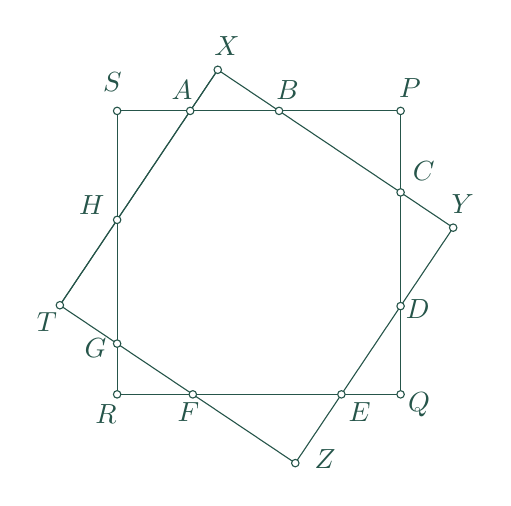
\begin{tikzpicture}[thachthuctoanhoc,scale=0.9]
			\draw  (0.,4.)-- (0.,0.);
			\draw  (0.,0.)-- (4.,0.);
			\draw  (4.,0.)-- (4.,4.);
			\draw  (4.,4.)-- (0.,4.);
			\draw  (1.42,4.58)-- (-0.8078121195006047,1.2578240323236605);
			\draw  (1.42,4.58)-- (-0.8078121195006047,1.2578240323236605);
			\draw  (-0.8078121195006047,1.2578240323236605)-- (2.514363848175734,-0.9699880871769437);
			\draw  (2.514363848175734,-0.9699880871769437)-- (4.742175967676339,2.352187880499395);
			\draw  (4.742175967676339,2.352187880499395)-- (1.42,4.58);
			\draw [fill=white] (0.,4.) circle (1.5pt);
			\draw (-0.06727272727272707,4.4018181818181805) node {$S$};
			\draw [fill=white] (0.,0.) circle (1.5pt);
			\draw (-0.15818181818181798,-0.2709090909090915) node {$R$};
			\draw [fill=white] (4.,0.) circle (1.5pt);
			\draw (4.26,-0.14363636363636423) node {$Q$};
			\draw [fill=white] (4.,4.) circle (1.5pt);
			\draw (4.132727272727273,4.329090909090908) node {$P$};
			\draw [fill=white] (1.42,4.58) circle (1.5pt);
			\draw (1.550909090909091,4.91090909090909) node {$X$};
			\draw [fill=white] (-0.8078121195006047,1.2578240323236605) circle (1.5pt);
			\draw (-0.9909090909088,1.02) node {$T$};
			\draw [fill=white] (2.514363848175734,-0.9699880871769437) circle (1.5pt);
			\draw (2.932727272727273,-0.9072727272727279) node {$Z$};
			\draw [fill=white] (4.742175967676339,2.352187880499395) circle (1.5pt);
			\draw (4.878181818181818,2.6927272727272724) node {$Y$};
			\draw [fill=white] (1.0310588235294116,4.) circle (1.5pt);
			\draw (0.9145454545454548,4.292727272727272) node {$A$};
			\draw [fill=white] (2.2849122807017546,4.) circle (1.5pt);
			\draw (2.4054545454545457,4.292727272727272) node {$B$};
			\draw [fill=white] (4.,2.849882352941175) circle (1.5pt);
			\draw (4.32727272727273,3.1472727272727266) node {$C$};
			\draw [fill=white] (4.,1.2454342444908202) circle (1.5pt);
			\draw (4.241818181818182,1.2018181818181812) node {$D$};
			\draw [fill=white] (3.164826447812038,0.) circle (1.5pt);
			\draw (3.423636363636364,-0.25272727272727336) node {$E$};
			\draw [fill=white] (1.0678903848416958,0.) circle (1.5pt);
			\draw (1.0054545454545456,-0.25272727272727336) node {$F$};
			\draw [fill=white] (0.,0.716114728658549) circle (1.5pt);
			\draw (-0.30363636363636337,0.6563636363636357) node {$G$};
			\draw [fill=white] (0.,2.4624561403508776) circle (1.5pt);
			\draw (-0.35818181818181793,2.674545454545454) node {$H$};
		\end{tikzpicture}
		\vspace*{-10pt}
	\end{figure}
	\begin{flushright}
		\textit{Nguyễn Thúy Quỳnh, Hà Nội (st)}
	\end{flushright}
	{\color{thachthuctoanhoc}{\usefont{T5}{qag}{b}{n} P797.}}
	(Mức $A$) Có bao nhiêu bộ sắp thức tự các số nguyên dương $(a,b,c)$ thỏa mãn $abc=2023^{2024}$.
	\begin{flushright}
		\textit{Vũ Hồng Sơn, Phú Thọ}
	\end{flushright}
	{\color{thachthuctoanhoc}{\usefont{T5}{qag}{b}{n} P798.}}
	(Mức $A$) Cho $f(x)$ là một đa thức hệ số thực có bậc là một số nguyên dương $n \ge 2$. Giả sử rằng, $f(x)$ có $n$ nghiệm thực là $ \alpha_{1},\cdots,\alpha_{n}$ và $f^\prime(x)$ có $n-1$ nghiệm thực là $\alpha_1^\prime,\ldots,\alpha_{n-1}^\prime$ (không nhất thiết phân biệt).  Chứng minh rằng
	\begin{align*}
		\prod_{\substack{1\le k,\ell \le n \\ k \ne \ell}}(\alpha_{k}-\alpha_{\ell})=n^{n}\prod_{\substack{1\le i \le n\\ 1\le j \le n-1}}(\alpha_{i}-\alpha'_{j}).
	\end{align*}
	(Chú ý: Các nghiệm của $f(x)$ và $f^\prime(x)$ không nhất thiết phân biệt).
	\begin{flushright}
		\textit{Dương Hồng Sơn, England }
	\end{flushright}
	{\color{thachthuctoanhoc}{\usefont{T5}{qag}{b}{n} P799.}}
	(Mức $A$) Tìm tất cả các số nguyên tố $p$ thoả mãn
	\begin{align*}
		\sum_{i=1}^{\left[\frac p2\right]} i \cdot C_p^i \equiv 0\pmod{p^2}.
	\end{align*}
	\begin{flushright}
		\textit{Trần Minh Hiền, Bình Phước}
	\end{flushright}
	{\color{thachthuctoanhoc}{\usefont{T5}{qag}{b}{n} P800.}}
	(Mức $A$) Cho tứ giác lồi $ABCD$ có $AB + CD > BC + DA$. Các đường chéo $AC$, $BD$ cắt nhau tại $O$. Gọi $x, y, z, t$ lần lượt là khoảng cách từ điểm $O$ đến các đường thẳng $AB, BC, CD, DA$. Chứng minh rằng 
	\begin{align*}
		\dfrac{1}{x} + \dfrac{1}{z} > \dfrac{1}{y} + \frac{1}{t}.
	\end{align*}
	\definecolor{ffqqqq}{rgb}{1,0,0}
	\definecolor{qqzzcc}{rgb}{0,0.6,0.8}
	\definecolor{qqqqff}{rgb}{0,0,1}
	\definecolor{qqqqffa}{rgb}{1,1,1}
	\begin{tikzpicture}[thachthuctoanhoc,scale=0.78]
		\draw[color=ffqqqq] (-1.933047864809872,1.6169496023416794) -- (-1.6595434766014723,1.6890283761294527) -- (-1.7316222503892453,1.9625327643378525) -- (-2.005126638597645,1.8904539905500792) -- cycle; 
		\draw[color=ffqqqq] (1.808456113111784,1.4401828355632256) -- (1.9130003775568354,1.177370170777749) -- (2.1758130423423117,1.2819144352228005) -- (2.0712687778972603,1.544727100008277) -- cycle; 
		\draw[color=ffqqqq] (-1.5358683620315439,-2.317157287525381) -- (-1.818711074506163,-2.317157287525381) -- (-1.818711074506163,-2.6) -- (-1.5358683620315439,-2.6) -- cycle; 
		\draw[color=ffqqqq] (-3.8368552706185506,0.4807837728633495) -- (-3.791839649886504,0.7600212952168265) -- (-4.071077172239981,0.8050369159488732) -- (-4.116092792972028,0.5257993935953962) -- cycle; 
		\draw  (-4.62,-2.6)-- (3.72,-2.6);
		\draw  (3.72,-2.6)-- (1.56,2.83);
		\draw  (1.56,2.83)-- (-3.98,1.37);
		\draw  (-3.98,1.37)-- (-4.62,-2.6);
		\draw  (-3.98,1.37)-- (3.72,-2.6);
		\draw  (-4.62,-2.6)-- (1.56,2.83);
		\draw [dashed,color=qqzzcc] (-2.005126638597645,1.8904539905500792)-- (-1.5358683620315436,0.10984381782665315);
		\draw [dashed,color=qqzzcc] (-1.5358683620315436,0.10984381782665315)-- (2.0712687778972603,1.544727100008277);
		\draw [dashed,color=qqzzcc] (-1.5358683620315436,0.10984381782665315)-- (-1.5358683620315439,-2.6);
		\draw [dashed,color=qqzzcc] (-4.116092792972028,0.5257993935953962)-- (-1.5358683620315436,0.10984381782665315);
		\draw (-1.84,1.55) node[anchor=north west] {$x$};
		\draw (0.58,1.05) node[anchor=north west] {$y$};
		\draw (-2,-1.01) node[anchor=north west] {$z$};
		\draw (-3.56,0.4) node[anchor=north west] {$t$};
		\draw [fill=white] (-3.98,1.37) circle (1.5pt);
		\draw[color=qqqqff] (-4.42,1.94) node {$A$};
		\draw [fill=white] (1.56,2.83) circle (1.5pt);
		\draw[color=qqqqff] (1.72,3.14) node {$B$};
		\draw [fill=white] (3.72,-2.6) circle (1.5pt);
		\draw[color=qqqqff] (3.64,-2.98) node {$C$};
		\draw [fill=white] (-4.62,-2.6) circle (1.5pt);
		\draw[color=qqqqff] (-4.74,-2.96) node {$D$};
		\draw [fill=white] (-1.5358683620315436,0.10984381782665315) circle (1.5pt);
		\draw[color=qqqqff] (-2.16,-0.1) node {$O$};
		\draw [fill=white] (-2.005126638597645,1.8904539905500792) circle (1.5pt);
		\draw [fill=white] (2.0712687778972603,1.544727100008277) circle (1.5pt);
		\draw [fill=white] (-1.5358683620315439,-2.6) circle (1.5pt);
		\draw [fill=white] (-4.116092792972028,0.5257993935953962) circle (1pt);
	\end{tikzpicture}
	\begin{flushright}
		\textit{George Apostolopoulos, Greece}
	\end{flushright}
\end{multicols}
\newpage
\centerline{{\large{\textbf{\color{thachthuctoanhoc}\color{thachthuctoanhoc}\color{thachthuctoanhoc}GIẢI BÀI KỲ TRƯỚC}}}}
\vspace*{-5pt}
\begin{multicols}{2}
	\setlength{\abovedisplayskip}{5pt}
	\setlength{\belowdisplayskip}{5pt}
	{\color{thachthuctoanhoc}{\usefont{T5}{qag}{b}{n} P761.}}
	(Mức $B$) Mỗi bạn An, Bình, Huệ, Nga đều có một khoản tiền tiết kiệm. Biết rằng, tiền tiết kiệm của tất cả các nhóm hai bạn, có thể lập được từ bốn bạn đó, là $1,9$ triệu đồng, $2,07$ triệu đồng, $2,11$ triệu đồng, $2,33$ triệu đồng, $2,5$ triệu đồng, và $x$ triệu đồng. Hãy tìm $x$.
	\vskip 0.05cm
	(Tiền tiết kiệm của một nhóm hai bạn là tổng tiền tiết kiệm của hai bạn đó.)
	\vskip 0.05cm
	\textbf{Lời giải} (\textit{dựa theo ý giải của bạn Lê Nguyễn Hoàng Nhật Đình, lớp $9$C, trường THCS Nguyễn Thái Bình, Tp. Cà Mau, tỉnh Cà Mau})\textbf{.}
	\vskip 0.05cm
	Gọi $a, b, c, d$ (triệu đồng), tương ứng, là số tiền tiết kiệm của các bạn An, Bình, Huệ, Nga.
	\vskip 0.05cm
	Theo giả thiết của bài ra, ta có:
	\begin{align*}
		\{a + b; a + c; a + d; b + c; b + d; c + d\} = \{1,9; 2,07; 2,11; 2,33; 2,5; x\}. \tag{$1$}
	\end{align*}
	Dễ thấy, có thể phân chia sáu số $a + b$, $a + c$, $a + d$, $b + c$, $b + d$, $c + d$ thành ba nhóm, mỗi nhóm hai số, sao cho các tổng hai số cùng nhóm bằng nhau (và cùng bằng $a + b + c + d$).
	\vskip 0.05cm
	Vì thế, theo ($1$), có thể phân chia sáu số $1,9$; $2,07$; $2,11$; $2,33$; $2,5$; $x$ thành ba nhóm, mỗi nhóm hai số, sao cho các tổng hai số cùng nhóm bằng nhau. \hfill ($2$)
	\vskip 0.05cm
	Suy ra, trong năm số $1,9$; $2,07$; $2,11$; $2,33$; $2,5$ phải có bốn số có tính chất: Có thể phân chia bốn số đó thành hai nhóm, mỗi nhóm hai số, sao cho các tổng hai số cùng nhóm bằng nhau. \hfill ($3$)
	\vskip 0.05cm
	Từ năm số nêu trên, có thể lập được năm nhóm bốn số. Bằng cách kiểm tra trực tiếp từng nhóm, trong năm nhóm đó, ta thấy chỉ có duy nhất nhóm bốn số $1,9$; $2,07$; $2,33$; $2,5$ có tính chất nêu ở ($3$); cụ thể, ta có:
	\begin{align*}
		1,9 + 2,5 = 2,07 + 2,33 = 4,4.
	\end{align*}
	Vì nhóm bốn số nói trên là nhóm duy nhất có tính chất nêu ở ($3$), nên từ đây và ($2$) suy ra, phải có
	\begin{align*}
		2,11 + x = 4,4;
	\end{align*}
	Vì thế, $x = 4,4 - 2,11 = 2,29$.
	\vskip 0.05cm
	Ta có điều cần tìm theo yêu cầu đề bài.
	\vskip 0.05cm
	\textbf{Bình luận và Nhận xét}
	\vskip 0.05cm	
	Trong số các lời giải Tạp chí đã nhận được từ bạn đọc, chỉ có hai lời giải đúng. Các lời giải còn lại là lời giải sai, do người giải bài đã ngộ nhận rằng, với các ký hiệu ở Lời giải trên và với giả sử $a + b = x$, ta có
	\begin{align*}
		(1) \Leftrightarrow \begin{cases}
			c\,\, + \,\,d\,\, \in \,\,\left\{ {1,9;\,\,2,07;\,\,2,11;\,\,2,33;\,\,2,5} \right\}\\
			x\,\, + \,\,c\,\, + \,\,d\,\, = \,\,\frac{{1,9\,\, + \,\,2,07\,\, + \,\,2,11\,\, + \,\,2,33\,\, + \,\,2,5\,\, + \,\,x}}{3}.
		\end{cases}
	\end{align*}
	\begin{flushright}
		\textbf{Nguyễn Khắc Minh}
	\end{flushright}
	{\color{thachthuctoanhoc}{\usefont{T5}{qag}{b}{n} P762.}}
	(Mức $B$) Cho tam giác $ABC$ với trọng tâm $G$. Dựng ra phía ngoài tam giác đó các tam giác $ABM$ và $ACN$, sao cho $\angle BAM = 45^\circ$, $AB = 3\sqrt{2}AM$, $\angle NAC = 90^\circ$, và $AC = 3AN$. Chứng minh rằng, $\angle GMN = 90^\circ$.
	\vskip 0.05cm  
	\textbf{Lời giải} (\textit{phỏng theo đa số lời giải Tạp chí đã nhận được từ bạn đọc})\textbf{.}
	\vskip 0.05cm
	
	%%%%
	Dựng ra phía ngoài tam giác $ABC$, tam giác $ABE$ vuông cân tại $E$, và tam giác $ACF$ vuông cân tại $A$.
	\vskip 0.05cm
	Gọi $I$ là trung điểm của $BC$; dựng hình bình hành $ABDC$.
	\vskip 0.05cm
	Từ việc dựng nêu trên và các giả thiết của bài ra, ta có:
	\vskip 0.05cm
	($i$) $M$ thuộc tia $AE$, và $\sqrt{2}AE = AB = 3\sqrt{2}AM$;
	\vskip 0.05cm 
	($ii$) $N$ thuộc tia $AF$, và $AF = AC = 3AN$;
	\vskip 0.05cm
	($iii$) $G$ thuộc tia $AD$, và $AG\,\, = \,\,\frac{2}{3}AI\,\, = \,\,\frac{2}{3} \cdot \left( {\frac{1}{2}AD} \right)\,\, = \,\,\frac{1}{3}AD$;
	\vskip 0.05cm
	($iv$) $BD = AC = AF$;
	\vskip 0.05cm
	($v$)  
	\begin{align*}
		\angle EBD\,\, = \,\,{45^{\rm{o}}}\, + \,\,\angle ABD\,\, = \,\,{45^{\rm{o}}}\, + \,\,\left( {{{180}^{\rm{o}}}\, - \,\,\angle CAB} \right)\,\, = \,\,{225^{\rm{o}}}\, - \,\,\angle CAB\\
			= \,\,\left( {{{360}^{\rm{o}}}\, - \,\,\left( {{{45}^{\rm{o}}}\, + \,\,{{90}^{\rm{o}}}} \right)} \right)\,\, - \,\,\angle CAB\\
			= \,\,{360^{\rm{o}}}\, - \,\,\left( {{{45}^{\rm{o}}}\, + \,\,\angle CAB\,\, + \,\,{{90}^{\rm{o}}}} \right)\,\, = \,\,\angle EAF.
	\end{align*}
	Từ ($i$) và ($ii$) suy ra, $M$ thuộc tia $AE$, $N$ thuộc tia $AF$, và $\dfrac{AM}{AE} = \frac{AN}{AF}$. Vì thế, theo định lý Thales,
	\begin{align*}
		MN \parallel EF.       \tag{$1$}                 
	\end{align*}                          
	Từ ($i$) và ($iii$) suy ra, $M$ thuộc tia $AE$, $G$ thuộc tia $AD$, và $\dfrac{AM}{AE} = \dfrac{AG}{AD}$  Vì thế, theo định lý Thales,
	\begin{align*}
		MG \parallel ED.  \tag{$2$}
	\end{align*}                  
	Từ ($1$) và ($2$) suy ra, hai góc $GMN$ và $DEF$ hoặc bằng nhau, hoặc bù nhau.                                           \hfill  ($3$)
	\vskip 0.05cm
	Tiếp theo, do tam giác $ABE$ cân tại $E$ nên $BE = AE$. Từ đây và ($iv$), ($v$), suy ra 
	\begin{align*}
		\Delta EBD = \Delta EAF.
	\end{align*}
	Do đó, $\angle BED = \angle AEF$. Vì thế
	\begin{align*}
		\angle DEF\,\, = \,\,\angle BEF\,\, - \,\,\angle BED\,\, = \,\,\left( {\angle BEA\,\, + \,\,\angle AEF} \right)\,\, - \,\,\angle BED\,\, = \,\,\angle BEA\,\, = \,\,{90^{\circ}}. \tag{$4$}
	\end{align*}
	Từ ($3$) và ($4$), suy ra  $\angle GMN = 90^\circ$.
	\vskip 0.05cm
	Ta có điều phải chứng minh theo yêu cầu đề bài.
	\vskip 0.05cm
	\textbf{Bình luận và Nhận xét}
	\vskip 0.05cm
	Tất cả các lời giải Tạp chí đã nhận được từ bạn đọc đều là lời giải đúng.
	\begin{flushright}
		\textbf{Hạ Vũ Anh}
	\end{flushright}
	{\color{thachthuctoanhoc}{\usefont{T5}{qag}{b}{n} P763.}}
	(Mức $B$) Cho một đa giác đều có $2024$ đỉnh; tại mỗi đỉnh, người ta viết một số nguyên dương không vượt quá $1011$. Chứng minh rằng, tồn tại bốn đỉnh $A$, $B$, $C$, $D$ của đa giác đó, sao cho $ABCD$ là một hình chữ nhật, và $a + b = c + d$; trong đó, $a$, $b$, $c$, $d$, tương ứng, là số được viết tại các đỉnh $A$, $B$, $C$, $D$.
	\vskip 0.05cm
	\textbf{Lời giải} (\textit{dựa theo ý giải của bạn Lê Nguyễn Hoàng Nhật Đình, lớp $9$C, trường THCS Nguyễn Thái Bình, Tp. Cà Mau, tỉnh Cà Mau})\textbf{.}
	\vskip 0.05cm
	Ký hiệu ($H$) là đa giác đều đã cho trong đề bài.
	\vskip 0.05cm
	Vì ($H$) là đa giác đều, nên nó có đường tròn ngoại tiếp; ký hiệu đường tròn này là ($O$).
	\vskip 0.05cm
	Vì đa giác đều ($H$) có $2024$ đỉnh nên ($O$) có $1012 (= 2024 : 2)$ đường kính đôi một khác nhau, mà mỗi đường kính đều có cả hai đầu mút là đỉnh của ($H$). Vì vậy, ($O$) có $1012$ đường kính, mà ở mỗi đầu mút của mỗi đường đều có ghi một số nguyên dương không vượt quá $1011$.
	\vskip 0.05cm
	Xét $1012$ đường kính vừa nêu trên.
	\vskip 0.05cm
	Gán cho mỗi đường kính một số, bằng trị tuyệt đối của hiệu của hai số được ghi ở hai đầu mút của đường kính ấy.
	\vskip 0.05cm
	Khi đó, do số được ghi ở mỗi đầu mút của mỗi đường kính là một số nguyên dương không vượt quá $1011$, nên mỗi đường kính được gán một số tự nhiên không vượt quá $1010 (= 1011 - 1)$.
	\vskip 0.05cm
	Từ đó, do trong phạm vi từ $0$ đến $1010$ chỉ có $1011$ số tự nhiên đôi một khác nhau, và $1012 > 1011$, nên trong các số đã gán cho $1012$ đường kính phải có ít nhất hai số bằng nhau. Nói cách khác, trong số $1012$ đường kính phải có hai đường kính được gán cùng một số; gọi hai đường kính này là ($I$), ($II$).
	\vskip 0.05cm
	Ký hiệu $a$, $c$, với $a \ge c$, là hai số được ghi ở hai đầu mút của ($I$); và gọi $A$ là đầu mút được ghi số $a$, $C$ là đầu mút được ghi số $c$.
	\vskip 0.05cm
	Ký hiệu $b$, $d$, với $d \ge b$, là hai số được ghi ở hai đầu mút của ($II$); và gọi $B$ là đầu mút được ghi số $b$, $D$ là đầu mút được ghi số $d$.
	\vskip 0.05cm
	Khi đó:
	\vskip 0.05cm
	-- Vì tất cả các đầu mút của ($I$) và ($II$) đều là đỉnh của ($H$), và vì ($I$), ($II$) là hai đường kính khác nhau của cùng một đường tròn, nên $A$, $B$, $C$, $D$ là bốn đỉnh của ($H$) và tứ giác $ABCD$ là một hình chữ nhật;
	\vskip 0.05cm
	-- $|a - c|$ và $|b - d|$, tương ứng, là số được gán cho đường kính $AC$ và đường kính $BD$. Do đó
	\begin{align*}
		a - c = |a - c| = |b - d| = d - b.
	\end{align*}
	Suy ra, $a + b = c + d$.
	\vskip 0.05cm
	Vì vậy, ta có điều phải chứng minh theo yêu cầu đề bài.
	\vskip 0.05cm
	\textbf{Bình luận và Nhận xét}
	\vskip 0.05cm
	Tất cả các bạn đọc đã gửi lời giải tới Tạp chí đều có ý tưởng giải đúng. Tuy nhiên, ngoại trừ bạn \textit{Lê Nguyễn Hoàng Nhật Đình}, tất cả các bạn còn lại đều diễn đạt rất chưa ổn quá trình triển khai thực hiện ý tưởng giải của mình. Chẳng hạn, có bạn đã viết: Ở hai đầu của đường kính có ghi hai số $x$, $y$, nên đường kính có độ dài là $|x - y|$; ...
	\begin{flushright}
		\textbf{Nguyễn Khắc Minh}
	\end{flushright}
	{\color{thachthuctoanhoc}{\usefont{T5}{qag}{b}{n} P763.}}
	(Mức $B$) Tìm tất cả các bộ ba số thực $(x, y, z)$ thỏa mãn: $x,\,\,y,\,\,z\,\, \in \,\,\left( {0;\,\,\frac{1}{2}} \right)$  và
	\begin{cases}
			\left( {3{x^2}\, + \,\,{y^2}} \right) \sqrt{1\,\, - \,\,4{z^2}} \,\, \ge \,\,z\\
			\left( {3{y^2}\, + \,\,{z^2}} \right)\sqrt {1\,\, - \,\,4{x^2}} \,\, \ge \,\,x\\
			\left( {cases3{z^2}\, + \,\,{x^2}} \right)\sqrt {1\,\, - \,\,4{y^2}} \,\, \ge \,\,y.
	\end{cases}
	Lời giải (dựa theo Đáp án của BBT Tạp chí).
	• Giả sử (x, y, z) là bộ ba số thực thỏa mãn các yêu cầu của đề bài.
	Do   nên từ bất đẳng thức thứ nhất của hệ đã cho trong đề bài, ta có:
	
	Suy ra
	(1)
	dấu “=” xảy ra khi và chỉ khi
	
	Bằng cách hoàn toàn tương tự, từ bất đẳng thức thứ hai, bất đẳng thức thứ ba của hệ đã cho trong đề bài, ta được:
	(2)
	dấu “=” xảy ra khi và chỉ khi
	
	(3)
	dấu “=” xảy ra khi và chỉ khi
	
	Cộng ba bất đẳng thức (1), (2), (3), vế theo vế, ta được:
	(4)
	dấu “=” xảy ra khi và chỉ khi dấu “=” xảy ra đồng thời ở (1), (2) và (3).
	Từ đó, do ở (4) xảy ra dấu “=” nên ở (1), (2), (3) phải đồng thời xảy ra dấu “=”.
	Từ các điều kiện cần và đủ để xảy ra dấu “=” ở mỗi bất đẳng thức (1), (2), (3), đã nêu ở trên, dễ thấy, dấu “=” đồng thời xảy ra ở ba bất đẳng thức đó khi và chỉ khi
	
	Như vậy, nếu (x, y, z) là bộ ba số thực thỏa mãn các yêu cầu của đề bài thì
	(5)
	• Ngược lại, bằng cách kiểm tra trực tiếp, dễ thấy, bộ ba số thực (x, y, z), được nêu ở (5), thỏa mãn các yêu cầu của đề bài.
	Vậy, có duy nhất bộ ba số thực cần tìm theo yêu cầu đề bài: bộ (x, y, z) được nêu ở (5).
	Bình luận và Nhận xét
	Tất cả các lời giải Tạp chí đã nhận được từ bạn đọc, rất tiếc, đều là lời giải sai, do người giải bài đã ngộ nhận rằng, không mất tính tổng quát, có thể giả sử x  y  z.
	Nguyễn Khắc Minh
	P765. (Mức B) Cho số nguyên dương n. Gọi A là tích tất cả các số nguyên dương không vượt quá 2n + 1, B là tích tất cả các số nguyên dương lẻ không vượt quá 2n + 1, và C là tích tất cả các số nguyên dương chẵn không vượt quá 2n. Chứng minh rằng,   không là số chính phương.
	Lời giải (dựa theo ý giải của bạn Đỗ Duy Quang, lớp 12T1, trường THPT chuyên Nguyễn Quang Diêu, tỉnh Đồng Tháp).
	Đặt  
	Do   (vì mỗi số đều là tích của các số nguyên dương), nên S là một số nguyên dương.
	Từ giả thiết của bài ra, hiển nhiên có A = BC.
	Do đó
	
	Theo giả thiết của bài ra, ta có:
	
	Từ đó, do   nên B - C \ge 1. Vì vậy, từ (1) ta được:
	(3)
	(2) và (3) cho thấy, số nguyên dương S nằm giữa hai số chính phương liên tiếp. Vì thế, S không là số chính phương.
	Ta có điều phải chứng minh theo yêu cầu đề bài.
	Bình luận và Nhận xét
	1. Lời giải trên cho thấy, bài đã ra là một trường hợp đặc biệt của kết quả sau:
	“Nếu x, y là các số nguyên dương, thỏa mãn x > y, thì
	
	không là số chính phương.”
	2. Lời giải của bạn Đỗ Duy Quang là lời giải duy nhất Tạp chí đã nhận được từ bạn đọc.
	Lưu Thị Thanh Hà
	P766. (Mức B) Cho a, b, c là các số dương. Chứng minh rằng
	
	Lời giải (của người chấm bài).
	Kí hiệu A là vế trái của bất đẳng thức cần chứng minh theo yêu cầu đề bài.
	Đặt
	
	Do a, b, c  0 (theo giả thiết) nên
	
	(theo bất đẳng thức Cauchy - Schwarz).
	Do a, b, c > 0 (giả thiết), nên
	
	Ta có điều phải chứng minh theo yêu cầu đề bài.
	Bình luận và Nhận xét
	1. Từ lời giải trên, dễ thấy, dấu “=” ở bất đẳng thức của đề bài xảy ra khi và chỉ khi a = b = c.
	2. Có nhiều hướng tiếp cận để chứng minh bất đẳng thức của đề bài. Các hướng được sử dụng nhiều trong các lời giải Tạp chí đã nhận được từ bạn đọc, là:
	- Đưa việc chứng minh bất đẳng thức của đề bài về việc chứng minh bất đẳng thức
	
	bằng cách đặt      
	- Sử dụng các bất đẳng thức
	
	
	3. Trong số các lời giải Tạp chí đã nhận được từ bạn đọc, rất tiếc, có một lời giải sai, do người giải bài đã mắc lỗi sai kiến thức cơ bản về bất đẳng thức.
	4. Kết quả dưới đây là một trong các khái quát có thể từ bài đã ra:
	Kết quả khái quát. Với mọi số thực dương a, b, c, và với mọi số thực không âm k, ta có:
	
	Bạn đọc có thể chứng minh kết quả trên, bằng cách sử dụng kết quả sau của Vasile Cirtoaje:
	“Với mọi số thực a, b, c, ta đều có:
	”
	Võ Quốc Bá Cẩn
	P767. (Mức A) Cho x, y, z là các số thực không âm, thỏa mãn   Chứng minh rằng
	
	Lời giải (của người chấm bài).
	Trong phần trình bày dưới đây, cụm từ “trung bình cộng - trung bình nhân” được viết tắt là “tbc - tbn”.
	Không mất tính tổng quát, giả sử x \ge y \ge z.
	Khi đó, (y - z)(y - x)  0; do đó
	
	Suy ra
	
	Vì thế
	
	Ta có điều phải chứng minh theo yêu cầu đề bài.
	Bình luận và Nhận xét
	1. Trong Lời giải trên, ta đã sử dụng bất đẳng thức Schur bậc ba ở dạng:
	
	2. Dễ thấy, dấu “=” ở bất đẳng thức của đề bài xảy ra khi và chỉ khi hai trong ba số x, y, z bằng   và số còn lại bằng 0.
	3. Ngoài cách đã trình bày ở Lời giải trên, còn có thể chứng minh bất đẳng thức
	
	bằng cách sử dụng đồng nhất thức
	
	và bất đẳng thức trung bình cộng - trung bình nhân.
	4. Bài đã ra là một bài toán khó. Hầu hết các lời giải Tạp chí đã nhận được từ bạn đọc đều khá cồng kềnh, có nhiều tính toán phức tạp.
	5. Trong số các lời giải Tạp chí đã nhận được từ bạn đọc, rất tiếc, có một lời giải sai, do người giải bài đã mắc lỗi sai kiến thức cơ bản về bất đẳng thức.
	Võ Quốc Bá Cẩn
	P768. (Mức A) Cho a là một số nguyên dương lẻ và không là số chính phương. Chứng minh rằng
	
	với mọi số nguyên dương m, n.
	Lời giải (dựa theo Đáp án của BBT Tạp chí).
	Giả sử, ngược lại, tồn tại các số nguyên dương m, n, sao cho
	(1)
	Đặt  
	Do a là số nguyên dương không chính phương (giả thiết), nên   và   là các số vô tỉ. Vì thế
	
	và do (1) nên
	
	Suy ra
	(2)
	(3)
	Cộng các bất đẳng thức kép (2) và (3), vế theo vế, ta được:
	
	suy ra
	
	là điều vô lí, do với a là số nguyên dương lẻ không chính phương,   là một số nguyên dương.
	Điều vô lý nhận được ở trên cho ta điều phải chứng minh theo yêu cầu đề bài.
	Bình luận và Nhận xét
	1. Bài đã ra là một trường hợp đặc biệt của kết quả kinh điển sau:
	“Nếu ,  là các số vô tỉ dương, có tổng nghịch đảo bằng 1 (tức  ), thì với mọi    ”
	Cụ thể, bạn sẽ thu được kết luận của bài đã ra, từ kết quả kinh điển nêu trên, khi chọn   và   với a là một số nguyên dương lẻ không chính phương.
	2. Trong số các lời giải Tạp chí đã nhận được từ bạn đọc, rất tiếc, có một lời giải sai, do người giải bài đã ngộ nhận rằng, với x, y là các số vô tỉ dương, nếu [x] = [y] thì x = y.
	Lưu Thị Thanh Hà
	P769. (Mức A) Cho tam giác không cân ABC nội tiếp đường tròn (O). Trên tiếp tuyến tại A của (O), lấy điểm K tùy ý, khác A. Một đường thẳng , đi qua K, cắt các đường thẳng BC, CA, AB, tương ứng, tại D, E, F. Chứng minh rằng, tâm đẳng phương của đường tròn đường kính EF, đường tròn đường kính DK và đường tròn (O) nằm trên đường thẳng .
	Lời giải (dựa theo lời giải của bạn Vương Khánh Toàn, lớp 11A1 Toán, trường THPT chuyên Tự nhiên, ĐH Khoa học Tự nhiên - ĐHQG Hà Nội).
	Gọi I, J, tương ứng, là trung điểm của EF, DK; ta có, I, J, tương ứng, là tâm đường tròn đường kính EF, đường tròn đường kính DK.
	Kí hiệu (I), (J), tương ứng, là đường tròn đường kính EF, đường tròn đường kính DK.
	Theo bài ra, ta phải chứng minh tâm đẳng phương của ba đường tròn (I), (J), (O) thuộc đường thẳng .
	Vì bài ra đề cập đường tròn đường kính EF, nên ta hiểu E, F phải là hai điểm phân biệt. Do đó, đường thẳng  phải không trùng với tiếp tuyến AK của (O). Vì vậy, chỉ có thể xảy ra hai trường hợp sau đối với vị trí của :
	-  đi qua tâm O của (O);
	-  không đi qua O và không trùng với AK.
	• Xét trường hợp 1:  đi qua tâm O của (O) (xem Hình 1).
	
	Hình 1
	Trong trường hợp này, hiển nhiên, ba điểm I, J, O thẳng hàng. Vì thế, ba đường tròn (I), (J), (O) không có tâm đẳng phương.
	• Xét trường hợp 2:  không đi qua O và không trùng với AK.
	Gọi M là giao điểm thứ hai, khác A, của (O) và đường tròn (AEF).
	
	Hình 2
	Ta có, M là điểm Miquel của tứ giác toàn phần BCEFAD. Do đó, M thuộc đường tròn (CDE). Vì vậy
	
	Suy ra, bốn điểm A, K, D, M cùng thuộc một đường tròn.
	Xảy ra hai trường hợp sau:
	• Trường hợp 2.1: AM \parallel  (xem Hình 3).
	
	Hình 3
	Trong trường hợp này, do AMDK và AMEF là các tứ giác nội tiếp, nên chúng là các hình thang cân. Do đó, I, J cùng thuộc đường trung trực của AM; suy ra, I  J và OI  . Vì thế, ba đường tròn (I), (J), (O) không có tâm đẳng phương.
	• Trường hợp 2.2: AM cắt  (xem Hình 2).
	Gọi T là giao điểm của AM và . Xét phương tích của T đối với các đường tròn, ta có:
	
	Do đó, T là tâm đẳng phương của ba đường tròn (I), (J), (O). Từ đây, do T thuộc  nên ta có điều phải chứng minh theo yêu cầu đề bài.
	Bình luận và Nhận xét
	1. Lời giải trên cho thấy, để đảm bảo tính chuẩn xác của một bài toán, kết luận của bài ra nên được phát biểu là: Chứng minh rằng, nếu đường tròn đường kính EF, đường tròn đường kính DK và đường tròn (O) có tâm đẳng phương thì tâm ấy nằm trên đường thẳng .
	2. Lời giải của bạn Vương Khánh Toàn là lời giải duy nhất, trong số các lời giải Tạp chí đã nhận được từ bạn đọc, đề cập đầy đủ các trường hợp có thể xảy ra đối với vị trí của đường thẳng .
	Hạ Vũ Anh
	P770. (Mức A) Cho phép thực hiện việc đổi chỗ các số hạng trong một hoán vị, theo qui tắc: Mỗi lần, lấy ra khỏi hoán vị tám số hạng tùy ý của nó, rồi lại xếp tám số hạng đó vào tám vị trí mà chúng đã nằm, nhưng theo thứ tự ngược lại.
	Hỏi, nhờ việc thực hiện liên tiếp một số hữu hạn lần phép đổi chỗ nói trên đối với hoán vị (1, 2, …, 2023) của 2023 số nguyên dương đầu tiên, ta có thể nhận được hoán vị (2023, 2022, …, 1) hay không?
	Lời giải (dựa theo ý giải của bạn Trần Minh Hoàng, lớp 11T1, trường THPT chuyên Hà Tĩnh, tỉnh Hà Tĩnh).
	Gọi   là phép đổi chỗ đã cho trong đề bài, và gọi   là phép đổi chỗ hai số hạng tùy ý trong một hoán vị.
	Giả sử n là một số nguyên dương lớn hơn 1, và   là một hoán vị của n số thực đôi một khác nhau.
	Ta gọi cặp số hạng   là một nghịch thế của hoán vị a, nếu i  j và  
	Với i, j là hai số khác nhau thuộc tập hợp {1; 2; …; n},   kí hiệu việc hoán đổi vị trí của   cho nhau, trong hoán vị a.
	Xét hoán vị   bất kì của 2023 số nguyên dương đầu tiên.
	Ta có các Nhận xét sau:
	Nhận xét 1. 
	Bình luận và Nhận xét
	1. Từ Lời giải trên dễ thấy, kết quả của bài ra không thay đổi, nếu trong giả thiết thay 8 bởi   với k là số nguyên dương tùy ý lớn hơn 1 và không vượt quá  
	2. Lời giải của bạn Trần Minh Hoàng là lời giải duy nhất Tạp chí nhận được từ bạn đọc.
	Nguyễn Khắc Minh
\end{multicols}


%	\newpage 
	
%	\thispagestyle{empty}
%	\begingroup 
%	\AddToShipoutPicture*{\put(0,0){\includegraphics[width=19.5cm]{thumoi.pdf}}}
%	\centering
%	\vspace*{0cm}
%	\endgroup
%	\newpage	
%	\pagestyle{empty}
%	
%	\setcounter{figure}{0}
%	\thispagestyle{cackithitoannone}
\pagestyle{cackithitoan}
\everymath{\color{cackithi}}
\graphicspath{{../cackithi/pic/}}
\blfootnote{\color{cackithi}$^1$Trường Phổ thông Năng khiếu, ĐHQG TpHCM.}
\begingroup
\AddToShipoutPicture*{\put(0,616){\includegraphics[width=19.3cm]{../bannercackithi}}}
\AddToShipoutPicture*{\put(52,522){\includegraphics[scale=1]{../tieude3.pdf}}}
\centering
\endgroup
\vspace*{190pt}

\begin{multicols}{2}
	Kỳ thi chọn học sinh giỏi quốc gia năm học $2023-2024$ đã diễn ra trong hai ngày $5, 6/1/2024$. Bài viết giới thiệu đề thi môn Toán của kỳ thi năm nay cùng một số bình luận và nhận định của tác giả bài viết về đề thi này.
	\vskip 0.1cm
	Đề thi năm nay có ưu điểm là đặt các vấn đề thú vị, không theo lối mòn, đặc biệt là không đi theo một mô--típ cũ suốt hơn mười năm nay là đề thi lúc nào cũng có hai bài hình. Điều này sẽ giúp cho việc dạy và học đều hơn, hướng đến cơ bản hơn, tránh bắt tủ. Tuy vậy, đề thi cũng có những nhược điểm về cấu trúc, diễn đạt và sắp xếp làm giảm đi đáng kể những điểm tích cực. Trước khi đi đến những đánh giá chung, chúng ta đi chi tiết vào từng bài toán thi.
	\vskip 0.1cm
	\textbf{\color{cackithi}Bài $\pmb1$:} Với mỗi số thực $x$, ta gọi $\lfloor x\rfloor$ là số nguyên lớn nhất không vượt quá $x$.
	\vskip 0.1cm
	Cho dãy số $\{a_n\}_{n=1}^\infty$ xác định bởi: $a_n = \dfrac{1}{4^{\lfloor-\log_4 n\rfloor}}, \forall n \ge 1$. Đặt $b_n =  \dfrac{1}{n^2}\left( {\sum\limits_{k = 1}^n {{a_k}}  - \frac{1}{{{a_1} + {a_2}}}} \right), \forall n \ge 1$. 
	\vskip 0.1cm
	$a)$ Tìm một đa thức $P(x)$ với hệ số thực sao cho $b_n = P\left(\dfrac{a_n}{n}\right), \forall n \ge 1$.
	\vskip 0.1cm
	\columnbreak
	$b)$ Chứng minh rằng tồn tại một dãy số nguyên dương $\{n_k\}_{k=1}^\infty$ tăng thực sự sao cho
	\begin{align*}
		\mathop {\lim }\limits_{k \to \infty } {b_{{n_k}}} = \frac{{2024}}{{2025}}. 
	\end{align*}
	Bài toán này có định dạng khá lạ so với các bài toán dãy số trong các kỳ thi năm trước, một dãy số dưới dạng tổng đòi hỏi phần xử lý đại số trước. Mặc dù đã có hướng dẫn trước để đi đến công thức mấu chốt
	\begin{align*}
		b_n = - \dfrac{1}{5}\left(\dfrac{a_n}{n}\right)^2 + \dfrac{a_n}{n}
	\end{align*}
	nhưng đây vẫn là một ý không hề hiển nhiên. Ý thứ hai thì không khó đối với một học sinh (hoặc sinh viên) được học bài bản về giới hạn và về tập số thực, nhưng với các em học sinh chỉ vừa làm quen với giải tích thì quả là quá tầm. 
	\vskip 0.1cm
	\textbf{\color{cackithi}Bài $\pmb2$:} Tìm tất cả các đa thức $P(x), Q(x)$ với hệ số thực sao cho với mỗi số thực $a$ thì $P(a)$ là nghiệm của phương trình: $x^{2023} + Q(a)\cdot x^2 + (a^{2024} + a)x + a^3 + 2025a = 0$.
	\vskip 0.1cm
	Đây là một bài phương trình hàm đa thức nhẹ nhàng, chủ yếu dựa vào sự chia hết, đồng dư đa thức.
	\vskip 0.1cm
	\textbf{\color{cackithi}Bài $\pmb3$:} Cho $ABC$ là tam giác nhọn với tâm đường tròn ngoại tiếp $O$. Gọi $A'$ là tâm của đường tròn đi qua $C$ và tiếp xúc $AB$ tại $A$, gọi $B'$ là tâm của đường tròn đi qua $A$ và tiếp xúc $BC$ tại $B$, gọi $C'$ là tâm đường tròn đi qua $B$ và tiếp xúc $CA$ tại $C$.
	\vskip 0.1cm
	$a)$ Chứng minh rằng diện tích tam giác $A'B'C'$ lớn hơn hoặc bằng diện tích tam giác $ABC$.
	\vskip 0.1cm
	$b)$ Gọi $X,Y,Z$ lần lượt là hình chiếu vuông góc của $O$ lên các đường thẳng $A'B',B'C', C'A'$. Biết rằng đường tròn ngoại tiếp tam giác $XYZ$ lần lượt cắt lại các đường thẳng $A'B', B'C', C'A'$ tại các điểm $X',Y',Z' (X' \ne X, Y' \ne Y, Z' \ne Z)$. Chứng minh rằng các đường thẳng $AX', BY', CZ'$ đồng quy.
	\vskip 0.1cm
	Bài toán hình học này khai thác một cấu hình khá thú vị, lời giải chủ yếu sử dụng phép biến đổi góc, tam giác đồng dạng. Bài này có hai ý khá độc lập nhưng đều có thể sử dụng chung phép đồng dạng (vị tự quay) biến $ABC$ thành $A'B'C'$. Đây là năm thứ hai xuất hiện bất đẳng thức hình học và nội dung này vẫn tiếp tục gây khó khăn cho các thí sinh. 
	\vskip 0.1cm
	\textbf{\color{cackithi}Bài $\pmb4$:} Người ta xếp $k$ viên bi vào các ô của một bảng $2024 \times 2024$ ô vuông sao cho hai điều kiện sau được thỏa mãn: mỗi ô không có quá một viên bi và không có hai viên bi nào được xếp ở hai ô kề nhau (hai ô được gọi là kề nhau nếu chúng có chung một cạnh).
	\vskip 0.1cm
	$a)$ Cho $k = 2024$. Hãy chỉ ra một cách xếp thỏa mãn cả hai điều kiện trên mà khi chuyển bất kỳ viên bi đã được xếp nào sang một ô tùy ý kề với nó thì cách xếp mới không còn thỏa mãn cả hai điều kiện nêu trên.
	\vskip 0.1cm
	$b)$ Tìm giá trị $k$ lớn nhất sao cho với mọi cách xếp $k$ viên bi thỏa mãn hai điều kiện trên ta có thể chuyển một trong số các viên bi đã được xếp sang một ô kề với nó mà cách xếp mới vẫn không có hai viên bi nào được xếp ở hai ô kề nhau.
	\vskip 0.1cm
	Bài $4$ là một bài cực trị tổ hợp có câu $a$ khá nhẹ nhàng, nhưng câu $b$ là một ý khó, dù không sử dụng kiến thức gì cao siêu nhưng tìm được $k$ đã khó, chứng minh lại càng khó hơn (một cách tiếp cận tự nhiên cho các bài toán kiểu thế này là thay $2024$ bằng một số nhỏ hơn để khảo sát). 
	\vskip 0.1cm
	\textbf{\color{cackithi}Bài $\pmb5$:} Với mỗi đa thức $P(x)$, ta đặt 
	\begin{align*}
		P_1(x) &= P(x), \forall x\in \mathbb{R};\\
		P_2(x) &= P\left(P_1(x)\right), \forall x\in \mathbb{R};\\
		&\ldots\\
		P_{2024}(x)&= P\left(P_{2023}(x)\right), \forall x \in \mathbb{R}.
	\end{align*}
	Cho $a$ là số thực lớn hơn $2$. Tồn tại hay không một đa thức $P(x)$ với hệ số thực thỏa mãn điều kiện: với mỗi $t\in (-a;a)$, phương trình $P_{2024} (x) = t$ có đúng $2^{2024}$ nghiệm thực phân biệt?
	\vskip 0.1cm
	Bài toán này khai thác một chủ đề truyền thống về nghiệm của đa thức. Bài này là bài nhẹ nhàng nhất của ngày $2$, chỉ cần bình tĩnh một chút sẽ thấy số $2024$ không có ý nghĩa gì ở đây, có thể thay bằng $n$ và từ đó thì sẽ nghĩ đến quy nạp. Với $n = 1$, một cách tự nhiên sẽ dẫn đến đa thức có dạng $x^2 - c$, với $c$ là hằng số dương. Bài này khai thác một ý không mới, nhưng phù hợp để đặt ở vị trí\linebreak Bài $5$.
	\vskip 0.1cm  
	\textbf{\color{cackithi}Bài $\pmb6$:} Với mỗi số nguyên dương $n$, gọi $\tau(n)$ là số các ước nguyên dương của $n$.
	\vskip 0.1cm
	$a)$ Giải phương trình nghiệm nguyên dương $\tau(n) + 2023 = n$ với $n$ là ẩn số.
	\vskip 0.1cm
	$b)$ Chứng minh rằng tồn tại vô số số nguyên dương $k$ sao cho có đúng hai số nguyên dương $n$ thỏa mãn phương trình $\tau(kn) + 2023 = n$. 
	\vskip 0.1cm
	Bài số học này khai thác một số tính chất cơ bản của hàm $\tau(n)$ -- số các ước số của số nguyên dương $n$. Bài này về ý tưởng thì nhẹ nhàng, phù hợp với một bài toán thi olympic, nhưng tính toán và xét trường hợp hơi phức tạp, nhất là trong bối cảnh thí sinh không được sử dụng máy tính cầm tay.
	\vskip 0.1cm 
	\textbf{\color{cackithi}Bài $\pmb7$:} Trong không gian, cho đa diện lồi $D$ sao cho tại mỗi đỉnh của $D$ có đúng một số chẵn các cạnh chứa đỉnh đó. Chọn ra một mặt $F$ của $D$. Giả sử ta gán cho mỗi cạnh của $D$ một số nguyên dương sao cho điều kiện sau được thỏa mãn: với mỗi mặt (khác mặt $F$) của $D$, tổng các số được gán với các cạnh của mặt đó là một số nguyên dương chia hết cho $2024$. Chứng minh rằng tổng các số được gán với các cạnh của mặt $F$ cũng là một số nguyên dương chia hết cho $2024$.
	\vskip 0.1cm
	Đây là bài tổ hợp có mô hình lý thuyết đồ thị. Với các thí sinh được học bài bản về lý thuyết đồ thị (đến mức có thể chuyển bài toán đề bài về bài toán đồ thị phẳng) thì Bài $7$ này còn nhẹ nhàng hơn Bài $4$. Nhưng ngược lại, nếu không được trang bị tốt thì chắc là cắn bút, nhất là trong áp lực của phòng thi. 
	\vskip 0.1cm
	Để bạn đọc cảm nhận được rõ hơn về đề thi cùng hướng giải, chúng tôi sẽ đi chi tiết hơn vào các bước giải cho các bài toán thi.
	\vskip 0.1cm
	Ở bài $1$, sau một lúc để định thần ta sẽ thấy dãy $a_n$ sẽ bắt đầu bởi $1$ số $1$, rồi $3$ số $4$, rồi $12$ số $16$ ... do ${a_n} = \frac{1}{{{4^{[ - {{\log }_4}n]}}}}$ nên một cách tự nhiên, ta chọn $s$ sao cho $4^s < n \le 4^{s+1}$  thì $a_n = 4^{s+1}$. Từ đó sẽ tính được tổng 
	\begin{align*}
			&\sum\limits_{i = 1}^n {a_i}\\
				 = &1 \!+\! (4 \!-\! 1)4 \!+\! (16 \!-\! 4){4^2} \!+\! ... \!+\! (n \!-\! {4^s}){4^{s \!+\! 1}} \\
			= &1 \!+\! 12\cdot(4^0 \!+\! 4^2 \!+\! ... \!+\! 4^{2s \!-\! 2}) \!+\! (n \!-\! 4^s)4^{s \!+\! 1}\\
			= &1 + \frac{3(4^{2s} - 1)}{5} + (n - 4^s)4^{s + 1}.
	\end{align*}
	Thay $4^s$ bởi $\frac{a_n}{4}$ vào và chú ý là  $\frac{1}{{{a_1} + {a_2}}} = \frac{1}{5}$  ta sẽ biến đổi về được ${b_n} =  - \frac{1}{5}{\left( {\frac{{{a_n}}}{n}} \right)^2} + \frac{{{a_n}}}{n}$. Ở ý $b)$, ta chỉ cần gọi $\alpha$ là nghiệm dương của phương trình  $- \frac{{{x^2}}}{5} + x = \frac{{2024}}{{2025}}$ và chứng minh tồn tại dãy con của dãy $\frac{a_n}{n}$  dần về $\alpha$. Với ý sau, chỉ cần dùng tính chất cơ bản sau đây về xấp xỉ:  $\lim \frac{{\lfloor{4^n}\alpha \rfloor}}{{{4^n}}} = \alpha$. 
	\vskip 0.1cm
	Ở bài $2$, từ điều kiện đề bài ta suy ra  $P(x)(P(x)^{2022} + Q(x)P(x) + x^{2024} + x) = - x(x^2+2025)$.
	\vskip 0.1cm
	Từ đây $P(x)$ là ước của $x(x^2+2025)$. Nếu $P(x)$ chia hết cho $x$ thì vế trái chia hết cho $x^2$, còn vế phải thì không, mâu thuẫn. Nếu $P(x) = k(x^2+2025)$ thì thay vào, ta suy ra $k(x^{2024}+x) + x$ chia hết cho $x^2 + 2025$. Sử dụng sự kiện $x^{2024} \equiv 2025^{1012} (\mod x^2 + 2025)$ ta sẽ suy ra ngay mâu thuẫn. Vậy chỉ còn lại trường hợp $P(x) = k$ với $k$ là hằng số, thay vào tính được $Q(x)$ tương ứng. 
	\vskip 0.1cm
	Ở bài $3$, ở câu $a)$ ta có thể chứng minh $\Delta CA'O \sim \Delta CAB$, suy ra $\frac{{{S_{COA'}}}}{{{S_{CAB}}}} = {\left( {\frac{{CO}}{{CB}}} \right)^2} = \frac{{{R^2}}}{{{a^2}}}$, từ đó  ${S_{C'OA'}} = {S_{COA'}} = \frac{{{R^2}}}{{{a^2}}} \cdot {S_{ABC}}$. Cùng các hệ thức tương tự, suy ra ${S_{A'B'C'}} = {S_{C'OA'}} + {S_{A'OB'}} + {S_{B'OC'}} = {S_{ABC}} \cdot {R^2}\left( {\frac{1}{{{a^2}}} + \frac{1}{{{b^2}}} + \frac{1}{{{c^2}}}} \right)$. Cuối cùng, sử dụng bất đẳng thức quen thuộc $a^2 + b^2 + c^2 \le 9R^2$ là hoàn tất chứng minh. Ở câu $b)$, ta chứng minh hai tam giác $ABC$  và $X'Y'Z'$  có các cạnh tương ứng song song bằng cách chẳng hạn $AB$  và $X'Y'$ cùng vuông góc với $OB'$. Khi đó $AX',BY',CZ'$  đồng quy tại tâm vị tự. 
	\vskip 0.1cm
	Với bài $4$, ta gọi một cách xếp $k$ viên bi là \textit{tốt} nếu nó thỏa mãn hai điều kiện đề bài và một cách xếp là \textit{cứng} nếu nó tốt nhưng nếu di chuyển bất kỳ một viên bi nào sang ô kề với nó thì cách xếp không còn tốt. Ý $a)$ là quá đơn giản vì ví dụ về đường chéo là rất hiển nhiên. Ở ý $b)$ điểm khó của bài toán nằm ở chỗ nếu có cách xếp cứng với $k$ viên bi thì chưa chắc đã có cách xếp cứng với $k+1$ viên bi. Ta cần tìm $k_0$ nhỏ nhất sao cho từ $k_0$  trở đi tồn tại cách xếp cứng. Được gợi ý bởi ý tưởng đường chéo, ta đưa ra thuật toán xây dựng cách xếp cứng cho mọi $k \ge 4046$ như sau. Đánh số các đường chéo song song với đường chéo chính là $D_1, D_2, \ldots, D_{4047}$. Đầu tiên ta đặt đầy bi vào hai đường chéo $D_{2022}$ và $D_{2026}$, cùng với hai viên bi ở đầu của đường chéo $D_{2024}$. Đây là một cách xếp cứng với $k = 4046$. Sau đó ta sẽ dùng các ô trên đường chéo chính $D_{2024}$ để tăng số bi dần dần (hành lang tạo bởi $D_{2022}$ và $D_{2026}$ sẽ đảm bảo tính cứng của cách xếp), khi đầy $D_{2024}$ rồi thì lại lấy bớt đi và thay bằng nguyên một đường chéo bên dưới (hay trên, cách $1$) đường chéo có bi. Như thế ta sẽ xây dựng được các cách xếp cứng cho mọi $k$ từ $4046$ cho đến $2024^2/2$. Với $k > 2024^2/2$ thì dễ dàng chứng minh sẽ phải có $2$ ô kề nhau, tức là không có cách xếp tốt. Để chứng minh $k = 4045$ là giá trị lớn nhất cần tìm gọi các ta tô màu các ô của hình vuông bằng hai màu đen trắng xen kẽ nhau. Ta lần lượt chứng minh các sự kiện sau $i)$ một cách xếp cứng sẽ chỉ có các viên bi trên các ô cùng một màu $ii)$ Nếu một cách xếp cứng có ít nhất $4045$ viên bi thì nó có ít nhất $4046$ viên bi. Ở ý $i)$ ta dùng phản chứng và nguyên lý cực hạn (xét hai đường chéo đen, trắng chứa bi gần nhau nhất), khi đó bi đứng đầu hàng của đường chéo ngắn hơn sẽ di chuyển được. Ở ý $ii)$, ta cũng sử dụng nguyên lý cực hạn, chọn ra đường chéo có chỉ số nhỏ nhất và lớn nhất có bi rồi chứng minh rằng toàn bộ các ô của $2$ đường chéo này đều có bi. Tiếp theo, ta phải cố gắng xử lý kỹ thuật, ``tránh" trường hợp toàn bộ đường chéo đều có bi ở câu $a)$. Câu $a)$ là một gợi ý quan trọng cho việc ``tránh" này. 
	\vskip 0.1cm
	Ở bài $5$, một cách tự nhiên ta nghĩ đến quy nạp. Điểm mấu chốt ở đây là ta phải làm mạnh mệnh đề lên thành $P_n(x)$ có $2^n$ nghiệm phân biệt thuộc $(-a, a)$ (lúc đó mới sử dụng giả thiết quy nạp được). Với $n = 1$, do tính đối xứng ta sẽ chọn $P(x) = P_1(x) = x^2 - c$. Để phương trình $P_1(x) = t$ có đúng $2$ nghiệm thực với mọi số thực $t \in (-a, a)$ ta sẽ cần có $c > a$ và để hai nghiệm này thuộc $(-a, a)$ ta cần có $c < a^2 - a$. Vì $a > 2$ nên chọn được $c$ như vậy. Đến đây thì mọi việc dễ dàng rồi:  $P_{k+1}(x) = 0 \Leftrightarrow P_k(P(x)) = 0$. Vì phương trình $P_k(x) = 0$ có $2^k$ nghiệm phân biệt thuộc $(-a, a)$ và ứng với mỗi nghiệm $x_i$ ấy phương trình $P(x) = x_i$ lại có $2$ nghiệm phân biệt dạng  $\pm\sqrt{x_i+c}$ nên dễ dàng suy ra phương trình $P_{k+1}(x)$ có $2^{k+1}$ nghiệm phân biệt.    
	\vskip 0.1cm
	Ở bài $6$, ý tưởng đầu tiên là sử dụng đánh giá $\tau (n) \le 2\sqrt n $  để chặn $n$. Bất đẳng thức này có thể chứng minh dễ dàng dựa vào nhận xét sơ đẳng: các ước số của $n$ chia thành các nhóm $(a, b)$ với $ab = n$. Từ đó áp dụng vào bài toán, ta suy ra được đánh giá $n < 2115$. Từ đây suy ra $2025 < n < 2115$ và như vậy $n$ không chính phương, suy ra $\tau(n)$ chẵn, suy ra $n$ lẻ. Dùng công thức tính $\tau(n) = (\alpha_1+1)\ldots(\alpha_r+1)$ với $n = p_1^{{\alpha _1}}...p_r^{{\alpha _r}}$  ta chứng minh được nếu $n$ lẻ và $2025 < n < 2115$ thì  $\tau(n) \le 18$  (chú ý do $3\cdot5\cdot7\cdot11\cdot13 > 2115$ nên $r \le 4$). Từ đây tiếp tục chặn được $n$ chặt hơn, thử các trường hợp ta đi đến kết luận không tồn tại $n$ sao cho  $\tau (n) + 2023 = n$. Với ý $b)$, ý tưởng cơ bản là chọn $k$ nguyên tố đủ lớn, khi đó thì $\tau (kn) \le \tau (k)\tau (n) \le 4\sqrt n$  từ đó cũng chặn được $n \le 2211$. Tương tự như ở trên, ta cũng đánh giá được $\tau(n) \le 18$. Lúc này do chọn $k$ nguyên tố lớn nên $(k, n) = 1$ và $\tau (kn) = \tau (k)\tau (n) = 2\tau (n)$. Vì $n$ không chính phương, $\tau(n)$ chẵn nên $n \equiv 3 \pmod 4$, từ đó thử từng trường hợp $n$ từ $2027$ đến $2059$ (cách $4$) ta tìm được đúng $2$ nghiệm là $2027$ và $2031$.
	\vskip 0.1cm 
	Ở bài $7$, đầu tiên ta chuyển mô hình đa diện thành mô hình đồ thị phẳng. Điều này có thể thực hiện bằng cách chiếu các đỉnh của đồ thị lên một mặt cầu nằm trong đa diện rồi dùng phép nghịch đảo có tâm $P$ (không trùng các đỉnh) nằm trên mặt cầu biến mặt cầu thành mặt phẳng. Sau đó ta xét đồ thị đối ngẫu của đồ thị phẳng, có đỉnh là các miền và hai miền có cạnh chung được sẽ được nối với nhau bởi một cạnh. Từ điều kiện đề bài suy ra đồ thị đối ngẫu cũng là đồ thị phẳng có các miền là các chu trình chẵn, từ đó chứng minh được mọi chu trình của nó đều chẵn, suy ra nó lưỡng phân, như vậy có thể tô màu các đỉnh bằng hai màu xanh, đỏ sao cho hai đỉnh kề nhau không cùng màu. Ngược trở lại với bài toán ban đầu, ta có thể tô màu các mặt của đa diện sao cho các mặt kề nhau không cùng màu. Đến đây thì mọi việc đơn giản. Giả sử $F$ được tô màu xanh. Xét $S_1$ là tổng các số viết trên các cạnh kề với mặt xanh khác $F$ và $S_2$ là tổng các số viết trên các cạnh kề với mặt đỏ. Vì mỗi cạnh không kề với $F$ sẽ xuất hiện trong cả hai tổng $S_1$ và $S_2$ đúng $1$ lần còn mỗi cạnh kề $F$ xuất hiện trong $S_2$ một lần nhưng không xuất hiện trong $F_1$. Từ đó tổng các số viết trên các cạnh kề với $F$ bằng $S_2 - S_1$. Vì mỗi cạnh chỉ kề với đúng một mặt xanh và một mặt đỏ nên $S_2$ chẳng qua là tổng các số trên các mặt đỏ và $S_1$ là tổng các số trên các mặt xanh khác $F$. Từ đây suy ra điều cần chứng minh.  
	\vskip 0.1cm
	Đề thi năm nay được đánh giá là khó, có nhiều bất ngờ gây ... sốc. Ở ngày thứ nhất, với bốn bài toán và bảy ý cần có sự sắp xếp và chọn lựa phù hợp hơn. Bài số $1$ nên là một bài nhẹ nhàng, chân phương thay vì những thách thức. Bài $1$ luôn là bài tạo tâm lý tốt (hay xấu) cho học sinh trong cả cuộc thi. Trước đây có một số năm cũng có Bài $1$ ``sát thủ" (như các năm $1997$, $2010$) và kết quả là năm đó học sinh làm bài kém hơn thường lệ, dù tổng thể đề không khó hơn. Vì ngày thứ nhất có đến bốn bài nên cũng nên cân nhắc về độ khó của các bài toán. So sánh giữa $5$ điểm của Bài $4$ với $6$ điểm của Bài $5$ thì thấy rõ sự khác biệt.
	\vskip 0.1cm
	Ngoài vấn đề về độ khó, đề thi năm nay còn có một số điểm thiếu hợp lý. Thứ nhất, đó là chọn chủ đề, hai bài toán đại số của đề thi đều thuộc chủ đề đa thức (đó là chưa kể Bài $1a$ cũng sử dụng từ đa thức). Đại số là phân môn có các chủ đề đa dạng nhất (đa thức, phương trình hàm, phương trình--hệ phương trình, bất đẳng thức, tổng và tích ...) và sở trường của các thí sinh ở mỗi phần cũng khác nhau nên đề thi không nên chọn trùng lặp. Thứ hai, trong đề thi năm nay, chủ đề tổ hợp xuất hiện trong hai bài. Điều này là tốt theo ý nghĩa sẽ khuyến khích học tổ hợp thay vì lâu nay luyện hình học hơi sâu. Nhưng vì hai bài này đều đặt ở vị trí cuối cùng của mỗi ngày nên chắc là sẽ rất ít học sinh đụng tới (vì về mặt tâm lý, gặp tổ hợp học sinh đã ngại, lại là bài cuối nên bỏ luôn). Đúng ra, nên chọn một bài dễ hơn (hoặc lấy Bài $7$ nhưng phát biểu chân phương hơn) để đặt lên vị trí đầu (Bài $1$ hoặc Bài $5$). Như năm $2012$ có hai bài tổ hợp thì Bài $5$ nhẹ nhàng và chân phương, mang tính khuyến khích rất cao.
	\vskip 0.1cm
	{\bf\color{cackithi} Thông tin cập nhật.} Sau khi bản thảo này đã được lên trang, Bộ Giáo dục và Đào tạo đã công bố kết quả kỳ thi học sinh giỏi Toán quốc gia. Kết quả đã phản ánh sát những lo ngại mà tác giả đã chỉ ra. Theo đó, có xấp xỉ $43 \%$ thí sinh đoạt giải, với các ngưỡng điểm đạt giải Nhất, Nhì, Ba và Khuyến Khích tương ứng là $22$, $16$, $11,5$ và $7$ (trên tổng số điểm tối đa là $40$). Đây là những con số thấp kỷ lục trong vòng nhiều năm trở lại đây. Với $31,5$ điểm, em Tạ Đức Anh, học sinh lớp $12$ trường THPT chuyên Đại học Sư phạm Hà Nội, là thủ khoa của kỳ thi. Ngoài ra, em Huỳnh Nguyên Phát, học sinh lớp $12$ trường THPT chuyên Chu Văn An, Bình Định, đã đem về giải Nhất đầu tiên của môn Toán cho tỉnh Bình Định. Bên cạnh đó, em Hà Nhật Minh, học sinh lớp $12$ trường THPT chuyên Lê Quý Đôn, Điện Biên cũng trở thành học sinh đầu tiên của tỉnh này đạt giải Nhì môn Toán, đồng thời lọt vào vòng thi chọn đội tuyển Toán tham dự kỳ thi IMO tới đây.
	\begin{figure}[H]
		\vspace*{-5pt}
		\centering
		\captionsetup{labelformat= empty, justification=centering}
		\includegraphics[height= 0.465\linewidth]{Ta_Duc_Anh}
		\includegraphics[height= 0.465\linewidth]{Huynh_Nguyen_Phat}
		\includegraphics[height= 0.465\linewidth]{Ha_Nhat_Minh}
		\caption{\small\textit{\color{cackithi}Từ trái sang phải: Tạ Đức Anh, Huỳnh Nguyên Phát và Hà Nhật Minh.}}
		\vspace*{-5pt}
	\end{figure}
\end{multicols}
\newpage
\begingroup
\AddToShipoutPicture*{\put(152,696){\includegraphics[scale=1]{../tieude1.pdf}}}
\centering
\endgroup
\vspace*{5pt}

\begin{multicols}{2}
	Trong phần đầu chuyên mục, chúng tôi sẽ trình bày với các bạn lời giải các bài toán trong kỳ thi Olympic toán vùng Trung Mỹ và Caribê năm $2023$ đăng trong số báo $11/2023$. 
	\begin{figure}[H]
		\vspace*{-5pt}
		\centering
		\captionsetup{labelformat= empty, justification=centering}
		\includegraphics[width= 0.85\linewidth]{gocolympic}
%		\caption{\small\textit{\color{}}}
		\vspace*{-15pt}
	\end{figure}
	{\bf\color{cackithi} OC$\pmb{55.}$} Tìm tất cả các cách tô màu các số nguyên dương sao cho điều kiện sau thỏa mãn:  
	\vskip 0.1cm
	$\bullet$ Mỗi số có màu xanh hoặc đỏ;
	\vskip 0.1cm
	$\bullet$  Tổng của hai số (không nhất thiết phân biệt) cùng màu bất kỳ có màu xanh.
	\vskip 0.1cm
	\textit{Lời giải.} Từ điều kiện bài toán ta suy ra tất cả các số chẵn có màu xanh. Hơn nữa nếu $2k+1$ là số lẻ đầu tiên có màu xanh thì tất cả các số lẻ tiếp theo đều có màu xanh do là tổng của 2 số màu xanh: 
	\begin{align*}
		2k+3&=(2k+1) + 2, 2k+5\\
		&=(2k+1) + 4, \cdots
	\end{align*}
	Như vậy cách tô màu thỏa mãn đầu bài có một trong hai dạng như sau:
	\vskip 0.1cm
	-- Tất cả các số chẵn tô màu xanh, tất cả các số lẻ tô màu đỏ.
	\vskip 0.1cm
	-- Các số lẻ $1, 3, \cdots, 2k-1 (k\ge 1)$ tô màu đỏ, tất cả các số còn lại tô màu xanh. 
	\vskip 0.1cm
	Có thể dễ dàng kiểm tra các cách tô này đều thỏa mãn điều kiện đầu bài.
	\vskip 0.1cm
	{\bf\color{cackithi} OC$\pmb{56.}$} Octavio viết một số nguyên dương $n$ lên bảng  và sau đó anh bắt đầu một quá trình trong đó, ở mỗi bước, anh xóa số nguyên $k$ được viết trên bảng  và thay thế nó bằng một trong các số sau:
	\begin{align*}
		3k-1, \quad 2k+1, \quad \frac{k}{2},
	\end{align*} 
	với điều kiện số mới viết là số nguyên.
	\vskip 0.1cm
	Chứng minh rằng với mọi số nguyên dương $n$, Octavio có thể viết lên bảng  số $3^{2023}$ sau hữu hạn bước.
	\vskip 0.1cm
	\textit{Lời giải.} Ta sẽ chứng minh bằng quy nạp theo $n.$ Ta có các nhận xét sau:
	\vskip 0.1cm
	Nhận xét $1$: Nếu $k$ lẻ, từ $k$ ta có thể nhận được $3k.$  Thật vậy 
	\begin{align*}
		 k\rightarrow 3k-1 \rightarrow \frac{3k-1}{2} \rightarrow 2\frac{3k-1}{2} +1=3k.
	\end{align*}
	Nhận xét $2$: Từ số $k$ ta có thể nhận được $3k+1.$  Thật vậy 
	\begin{align*}
		k&\rightarrow 2k+1 \rightarrow 3(2k+1)-1=6k+2 \\
		&\rightarrow \frac{6k+2}{2}=3k+1.
	\end{align*}
	Theo Nhận xét $1$, xuất phát từ số $1$ ta sẽ nhận được số $3^{2023},$ tức là khẳng định đúng với $n=1.$ Giả sử khẳng định đúng với mọi số $k< n,$ ta chứng minh nó cũng đúng với $n.$ 
	\vskip 0.1cm
	Nếu $n$ chẵn, ta viết được $\frac{n}{2}$ và áp dụng giả thiết quy nạp, ta có điều cần chứng minh. Với $n$ lẻ, ta viết được $3n-1$ và $3n+1$ (theo Nhận xét $2$). Chú ý rằng trong hai số chẵn liên tiếp  $3n-1$ và $3n+1$ phải có ít nhất một số chia hết cho $4,$ như vậy ta sẽ viết được một số nhỏ hơn $n$ là $\frac{3n-1}{4}$ hoặc $\frac{3n+1}{4}.$ Từ đó áp dụng quy nạp ta có điều phải chứng minh.
	\vskip 0.1cm
	{\bf\color{cackithi} OC$\pmb{57.}$} Trong một cái ao có $n (n \geq 3)$  hòn đá  xếp thành vòng tròn. Một công chúa muốn đánh số những hòn đá với các số $1, 2, \dots, n$ theo thứ tự nào đó rồi đặt một số con cóc lên những hòn đá. Sau khi đặt tất cả các con cóc vào vị trí, chúng bắt đầu nhảy theo quy tắc sau: khi một con cóc đến hòn đá có đánh số $k$, nó đợi $k$ phút rồi nhảy sang hòn đá liền kề theo chiều kim đồng hồ.
	\vskip 0.1cm
	Hỏi số lượng cóc nhiều nhất là bao nhiêu để công chúa có thể đánh số các hòn đá và đặt các con cóc sao cho không bao giờ có hai con cóc ở trên cùng một hòn đá trong thời gian từ một phút trở lên?
	\vskip 0.1cm
	\textit{Lời giải.}
	Ta nói hai con cóc gặp nhau nếu chúng ở trên cùng một hòn đá trong thời gian từ một phút trở lên. Ký hiệu $a_1, a_2, \dots, a_n$ là số của các hòn đá lần lượt theo chiều kim đồng hồ. Chúng ta coi các chỉ số modulo $n,$ tức là $a_{n+i}\equiv a_i.$ 
	\vskip 0.05cm
	Trước tiên ta chứng minh nhận xét sau: Giả sử có các con cóc trên hòn đá số $a_l$ và $a_k,$ khi đó chúng sẽ không bao giờ gặp nhau nếu và chỉ nếu $a_l+a_{l+1}+\dots+a_{k-1}\ge a_m $ với mọi $1\le m\le n.$
	\vskip 0.05cm
	{\it Chứng minh:} Giả sử hai con cóc không bao giờ gặp nhau. Nếu tồn tại $m$ để $a_l+a_{l+1}+\dots+a_{k-1}< a_m $ thì 
	\begin{align*}
		&a_l\!+\!a_{l\!+\!1}\!+\!\dots\!+\!a_{k\!-\!1}\!+\!a_k\!+\! a_{k\!+\!1}\!+\!\dots \!+\!a_{m\!-\!1} \\
		<\, &a_k\!+\! a_{k\!+\!1}\!+\!\dots \!+\!a_{m\!-\!1}\!+\!a_m.
	\end{align*} 
	Như vậy hai con cóc sẽ gặp nhau tại hòn đá $a_m$ sau $a_l+a_{l+1}+\dots+a_{m-1}$ phút và dẫn đến mâu thuẫn. 
	\vskip 0.05cm
	Chiều ngược lại giả sử $a_l+a_{l+1}+\dots+a_{k-1}\ge a_m $ với mọi $1\le m\le n.$ Nếu hai con cóc gặp nhau tại hòn đá $a_m$ thì ta có $a_l+\dots a_{k-1}+a_k+\dots +a_{m-1} < a_k+\dots +a_{m-1}+a_m$ và điều này dẫn đến mâu thuẫn. 
	\vskip 0.05cm
	Ta sẽ chứng minh số lượng cóc nhiều nhất có thể là $ \left\lceil \frac{n}{2} \right\rceil.$ Thật vậy, nếu công chúa đặt $ \left\lceil \frac{n}{2} \right\rceil+1$ con cóc. Với mỗi con cóc ở hòn đá $a_i$ ta xét hòn đá $a_{i+1}.$ Phải có ít nhất $2$ giá trị $i$ mà hòn đá $a_{i+1}$ cũng có cóc vì nếu trái lại thì có ít nhất $ \left\lceil \frac{n}{2} \right\rceil$ hòn đá trống và điều này mâu thuẫn vì dẫn đến số cóc bé hơn $\left\lceil \frac{n}{2} \right\rceil+1.$ Ta suy ra phải có số $a_i<n$ mà trên cả hai hòn đá $a_i$ và $a_{i+1}$ đều có cóc. Như vậy, theo nhận xét trên thì hai con cóc trên đó sẽ gặp nhau tại hòn đá có số $n,$ điều này mâu thuẫn với giả thiết.
	\vskip 0.1cm
	Bây giờ giả sử có $ \left\lceil \frac{n}{2} \right\rceil$ con cóc. Công chúa đánh số các hòn đá lần lượt theo chiều kim đồng hồ như sau:
	\begin{align*}
		n, 1, n-1, 2, n-2, \dots k, n-k, \dots.
	\end{align*}
	Nếu công chúa đặt các con cóc vào hòn đá số $n$ và các hòn số $k<\frac{n}{2}$ thì điều kiện trong nhận xét thỏa mãn và các con cóc không bao giờ gặp nhau. Như vậy số lượng cóc nhiều nhất có thể xếp là $ \left\lceil \frac{n}{2} \right\rceil.$
	\vskip 0.1cm
	Trong phần cuối của chuyên mục kỳ này, chúng tôi sẽ giới thiệu với bạn đọc các bài toán chọn lọc trong kỳ thi Olympic toán học trẻ của Hàn Quốc năm $2023$. Các bài toán này phù hợp với trình độ học sinh lớp $8-10$.
	\vskip 0.1cm
	{\bf\color{cackithi} OC$\pmb{64}$.} Tìm tất cả các cặp số nguyên $(x, y)$ thỏa mãn
	\begin{align*}
		y^2 = x^3 + 2x^2 + 2x + 1.
	\end{align*}
	{\bf\color{cackithi} OC$\pmb{65}$.} Cho $n (n\geq 5) $ là một số nguyên dương. Có $n$ viên đá trắng và $n$ viên đá đen (tổng cộng $2n$ viên) xếp thành một hàng trong đó $n$ viên đầu tiên có màu trắng và $n$ viên tiếp theo có màu đen.
	\begin{figure}[H]
		\vspace*{-5pt}
		\centering
		\captionsetup{labelformat= empty, justification=centering}
		\includegraphics[width= 0.7\linewidth]{OC65}
%		\caption{\small\textit{\color{}}}
		\vspace*{-10pt}
	\end{figure}
	Ta có thể thực hiện thao tác sau: chọn một số nguyên dương bất kỳ $k (k \leq 2n - 5)$ và  đổi chỗ viên đá ở vị trí thứ $k$ với viên đá ở vị trí thứ  $(k+5).$ 
	\vskip 0.1cm
	Tìm tất cả các số nguyên dương $n$ sao cho chúng ta có thể làm cho $n$ viên đá đầu tiên có màu đen và   $n$ viên đá tiếp theo có màu trắng sau một số hữu hạn lần thao tác.
	\vskip 0.1cm
	{\bf\color{cackithi} OC$\pmb{66}$.} Có $2023$ tay vợt  tham gia  một giải đấu quần vợt theo thể thức vòng tròn, hai tay vợt bất kỳ đấu với nhau đúng một trận. Biết rằng không có trận hòa và không có tay vợt nào thắng tất cả các tay vợt khác. Ta  gọi tay vợt $A$ là ``có kỹ năng" nếu với mỗi tay vợt $B$ thắng $A$, có một tay vợt $C$ thắng $B$ và thua $A$.
	\vskip 0.1cm
	Biết rằng có đúng $N (N\geq 0)$ tay vợt ``có kỹ năng". Tìm giá trị nhỏ nhất của $N$.	
\end{multicols}

%	\newpage
	
%	\setcounter{figure}{0}
%	\thispagestyle{lichsutoanhocnone}
\pagestyle{lichsutoanhoc}
\graphicspath{{../lichsutoanhoc/pic/}}
\everymath{\color{lichsutoanhoc}}
\blfootnote{$^1$\color{lichsutoanhoc}THPT chuyên Hà Nội -- Amsterdam.}
\begingroup
\AddToShipoutPicture*{\put(0,616){\includegraphics[width=19.3cm]{../bannerlichsu}}}
\AddToShipoutPicture*{\put(96,520){\includegraphics[scale=1]{../tieude4.pdf}}}
\centering
\endgroup

\vspace*{185pt}

\begin{multicols}{2}
	Để đảm bảo cho cuộc hành trình phía trên suôn sẻ, chúng tôi đã lược bớt một số chi tiết nhỏ để những bài viết cô đọng hơn. Bài viết này là chặng cuối của chuyến đi, cũng là một số tổng kết và những cái tên để những độc giả hứng thú có thêm nguồn tham khảo. Tất nhiên hành trình của chúng ta mới chỉ là thuật lại bước đầu chật vật khẳng định vị thế của hình học phi Euclid, và hành trình của lĩnh vực nghiên cứu này vẫn còn hết sức rộng mở phía trước.
	\vskip 0.1cm
	\textbf{\color{lichsutoanhoc}Đôi lời về các tiên đề:}
	\vskip 0.1cm
	Tiên đề không phải sự thật tự nó hiển nhiên, nó đơn thuần là luật chơi của thế giới đó. Và vì thế có hơn một hệ tiên đề diễn tả cùng loại hình học Euclid ta biết. Nổi tiếng nhất là luận án Grundlagen der Geometrie (Nền tảng của hình học) của nhà tiên phong, nhà thông thái David Hilbert $(1862-1943)$ trong một nỗ lực thống nhất các ngành toán học với nhau. Công trình với $21$ tiên đề và $6$ khái niệm nguyên thủy (Euclid đưa ra $5$ tiên đề, $0$ định nghĩa nguyên thủy) của ông có tinh thần khá tương đồng với cách phát triển của Euclid. 
	Ngoài ra ta có các đóng góp đến từ G. Peano, M. Pieri, G. Veronese, O. Veblen, G. de B. Robinson, E. V. Huntington, H. G. Forder, và G. Birkhoff. Chẳng hạn như cách lập tiên đề của Pieri chỉ có hai khái niệm nguyên thủy là ``điểm" và ``chuyển động".
	\vskip 0.1cm
	\textbf{\color{lichsutoanhoc}Hình học hyperbolic khác hình học Euclid như thế nào?}
	\vskip 0.1cm
	Công chuẩn bị của chúng ta từ đầu giờ đây sẽ có ích. Khi mà tiên đề song song đã không còn đúng, những mệnh đề tương đương với nó cũng vậy, từ ấy ta có những kết quả đáng chú ý như dưới đây. 
	Góc ở đỉnh của tứ giác Saccheri và góc thứ tư của tứ giác Lambert không phải góc vuông, mà là góc nhọn. Thậm chí hình chữ nhật còn không tồn tại trong thế giới này. Diện tích các tam giác bị chặn. Cả Bolyai và Lobachevsky đều phát hiện ra rằng diện tích tam giác trong hình học này tỉ lệ thuận với độ lệch -- hiệu của pi với tổng ba góc trong tam giác đó tính theo radian. Không tồn tại hai tam giác đồng dạng nhưng không bằng nhau nữa. Nói cách khác, hai tam giác đồng dạng thì bằng nhau. 
	\vskip 0.1cm
	Một hệ quả của điều này là chúng ta không thể định nghĩa các hàm lượng giác như trong hình học Euclid. Các hàm $\sin$, $\cos$ quen thuộc giờ được định nghĩa thông qua chuỗi lũy thừa Đồng thời có hai hàm hyperbolic hữu ích mà người ta cũng nghiên cứu ở đây là $\sinh$ và $\cosh$, có chuỗi lũy thừa giống của $\sin$ và $\cos$ bỏ đi $(-1)^n$, hay viết gọn lại thông qua hàm mũ cơ số $e$: 
	\begin{align*}
		&\cos(x) =  1 - \frac{x^2}{2!} + \frac{x^4}{4!} - ... \\
		&\sin(x) =  x - \frac{x^3}{3!} + \frac{x^5}{5!} - ... \\
		&\cosh(x) =  1 + \frac{x^2}{2!} + \frac{x^4}{4!} + ... \\
		&\sinh(x) =  x + \frac{x^3}{3!} + \frac{x^4}{4!} - ... 
	\end{align*}
	Giờ đây không phải có một mà là hai đường gọi là đường song song giới hạn (limiting parallel). Cụ thể, với điểm $P$ và đường thẳng $l$ không đi qua nó, sẽ tồn tại hai đường thẳng $d_1, d_2$ đối xứng nhau qua đường vuông góc $d$ hạ từ $P$ xuống $l$. Hai đường này là hai đường tạo với $d$ góc nhỏ nhất mà song song với $l$. 
	\vskip 0.1cm
	Và cuối cùng, hằng số $\pi$  không thể được định nghĩa như ở hình Euclid, bởi chu vi của đường tròn chia cho bán kính của nó trong không gian này còn chẳng phải một tỉ số cố định. Những điều trông rất hợp lý trong hình học Euclid, chẳng hạn như tỉ lệ giữa chu vi và bán kính của mọi đường tròn là như nhau, lại không đúng ở đây. Trong không gian hình học hyperbolic độ cong $-1$, chu vi của đường tròn bán kính $r$ được tính theo công thức: $C = 2\pi\cdot\sinh r$. 
	\vskip 0.1cm
	\textbf{\color{lichsutoanhoc}Hình học elliptic khác hình học Euclid như thế nào?}
	\vskip 0.1cm
	Theo cách thiết lập tiên đề theo hướng của Euclid, ta sẽ không thể thay thế được tiên đề $5$ bằng ``mọi đường thẳng đều cắt nhau" ngay. Bởi kết hợp định lý $16$ và $27$ thì ta thấy là đường song song tồn tại. Mặt khác, nhìn vào mô hình nửa mặt cầu của mặt phẳng elliptic ta đã dựng, việc một điểm nằm giữa hai điểm khác trông hơi sai sai, vì ``đường thẳng" ở mô hình này trông như những đường tròn. Vì thế các tiên đề về sự nằm giữa sẽ được thay thế bằng các tiên đề về sự phân cách (separation axiom). Một số điểm khác biệt so với hình học Euclid của hình học elliptic cũng tương tự như với hình học hyperbolic. Trong hình học elliptic, diện tích của một tam giác sẽ bị chặn và tỉ lệ thuận với hiệu của tổng ba góc tam giác đó (vẫn theo radian) với $\pi$, hai góc ở đỉnh của tứ giác Saccheri và góc thứ tư của tứ giác Lambert đều là góc tù. Không còn những tam giác đồng dạng nhưng không bằng nhau, vì thế hàm lượng giác cứ phải định nghĩa bằng chuỗi lũy thừa. Tất nhiên đây sẽ còn là một thế giới xa lạ với ta hơn cả hình hyperbolic, bởi cả quan hệ nằm giữa đã cần sửa thành sự phân tách để các tiên đề không dẫm vào chân nhau.
	\vskip 0.1cm
	\textbf{\color{lichsutoanhoc}Đóng góp của Riemann và di sản của hành trình}
	\vskip 0.1cm
	Những ý tưởng mà Bolyai và Lobachevsky đã thúc đẩy là khá mới mẻ với giới tri thức đương thời. Dù vậy, thời gian đã dần xua tan những nghi ngờ còn sót lại của đại đa số học giả. Người ta dần học được vài điều. Những tiên đề không phải là chân lý hay sự thật vĩnh cửu, chúng chỉ là những quy ước con người đề ra. Khi thay đổi các tiên đề thì ta sẽ tạo ra các hệ thống kết quả khác nhau, chúng ta sẽ không nghi ngờ liệu nó có đúng trong thực tế hay không, mà sẽ đi vào phát triển những hệ thống cho ra những kết quả thú vị, hoặc để tìm ra một mâu thuẫn nào đó để bác bỏ hệ thống đó.
	\vskip 0.1cm
	Như đã hứa, ta cùng quay ngược thời gian về ngày $10/6/1854$, Gottingen. Trong căn phòng nơi bài Habilitation lecture diễn ra, hầu hết các thính giả đều không hiểu gì mấy, thậm chí cả trưởng khoa Toán ngồi nghe còn có phần lúng túng. Bài nói chuyện là về Hình học, nhưng trên bảng không có lấy một hình vẽ nào. Phải đến $10$ năm sau giới Toán học mới dần vỡ ra ý nghĩa của những gì diễn ra ngày hôm ấy: đến tận 1868 những nội dung được bàn luận mới được đưa ra rộng rãi. Riêng việc bài nói vượt xa kỳ vọng của trưởng khoa Gauss thôi đã chứng thực cho sự kỳ tài của giảng viên trẻ Bernhard Riemann rồi. Và bởi vì đi sâu vào chi tiết còn hơi quá tầm với cả những thính giả hôm ấy, chúng ta sẽ chỉ đi qua những ý tưởng chính Riemann đã phát triển, bắt đầu với khái niệm độ cong.
	\vskip 0.1cm
	Đầu tiên, xét một đường cong bất kỳ trên mặt phẳng Euclid. Với một điểm $P$ nằm trên đường cong, cho hai điểm $Q$, $R$ tiến dần về $P$, khi đó đường tròn ngoại tiếp tam giác $PQR$ sẽ có giới hạn là đường tròn mật tiếp của đường cong tại $P$. Nếu đường tròn đó có bán kính $r$, thì độ cong của đường cong đó tại $P$ sẽ là $k = 1/r$ hoặc $k =  -(1/r)$, tùy vào việc đường tròn đó nằm về phía nào so với đường cong.
	\vskip 0.1cm
	Tiếp theo ta đến với đường cong bất kỳ trong không gian ba chiều. Đường tròn mật tiếp khi này nằm trên mặt phẳng Pi nào đó (ta gọi là mặt phẳng mật tiếp), và độ cong $k$ giờ trở thành một vectơ tại $P$, hướng về tâm đường tròn mật tiếp, độ lớn $1/r$
	\vskip 0.1cm
	Giờ ta đến với một bề mặt $S$ bất kỳ trong không gian ba chiều. Trong trường hợp này, một bề mặt được gọi là có thể định hướng được nếu nó có hai mặt, mỗi mặt hướng về một phía khác nhau. Cho dễ hiểu: Một tờ giấy là một mặt phẳng định hướng được, còn một dải Mobius thì không. Giả sử $S$ định hướng được. Nếu $d$ là một đường cong trên $S$, thì ở mỗi điểm $P$ trên gamma ta định nghĩa được một độ cong $k$.
	\vskip 0.1cm
	Gọi đường thẳng đi qua $P$, vuông góc với mặt phẳng tiếp tuyến tại $P$ là $N$. Xét một mặt phẳng chứa $N$ nào đó. Giao tuyến của mặt phẳng đó với $S$ là một đường cong (nằm trên mặt). Mỗi đường cong này có một độ cong khác nhau tại điểm $P$. Euler đã chứng minh những độ cong khác nhau này có giá trị lớn nhất và giá trị nhỏ nhất. Hai đường cong tương ứng với hai giá trị này được gọi là các đường cong chính (principle curve), và Euler chứng minh được hai đường cong chính sẽ vuông góc với nhau nếu chúng phân biệt. Tích độ cong của hai đường cong này được gọi là độ cong Gauss. 
	\begin{figure}[H]
		\vspace*{5pt}
		\centering
		\captionsetup{labelformat= empty, justification=centering}
		\includegraphics[width= 1\linewidth]{saddle point and riemann curvature.png}
		\caption{\small\textit{\color{lichsutoanhoc}Hai đường cong chính được tô màu đen trên hình. Nguồn: Greenberg}}
		\vspace*{-10pt}
	\end{figure}
	Gauss đã chứng minh được rằng độ cong Gauss K không thay đổi khi các bề mặt bị ``bẻ cong", miễn là sự bẻ cong ấy không thay đổi độ dài địa phương của cung và góc của những đường cong trên bề mặt ấy. 
	\vskip 0.1cm
	Ý tưởng này, cùng với ý tưởng về khoảng cách tổng quát trong các chiều không gian cao hơn và trên các bề mặt không tuân theo các tiên đề của Euclid, chính là cơ sở cho những không gian phi Euclid tổng quát hơn, và cả một lý thuyết Vật lý quan trọng nhất nhì thế kỉ hai mươi.
	\vskip 0.1cm
	$60$ năm sau bài nói chuyện vượt thời gian của Riemann tại Gottingen, một lý thuyết mới đã làm khuynh đảo Vật Lý đương thời -- Thuyết Tương đối của Einstein. Thuyết Tương đối rộng còn chỉ ra rằng thời gian và không gian có thể bị cong dựa vào khối lượng vật chất tại một vị trí. Vì vậy, hình học của lý thuyết ấy, hóa ra, lại chẳng phải hình Euclid, mà là hình học mà những Bolyai, Lobachevsky và Riemann phát triển. Một cách kiểm chứng rực rỡ cho những gì những con người tiên phong ấy đã viết nên.
	\vskip 0.1cm
	\textbf{\color{lichsutoanhoc}Tài liệu tham khảo}
	\vskip 0.1cm
	[$1$] E.T.  Bell, \textit{Men of Mathematics The Lives and Achievements of the Great Mathematicians from Zeno to Poincaré}.   
	\vskip 0.1cm
	[$2$] David M. Burton. \textit{The History of Mathematics An Introduction}. 
	\vskip 0.1cm
	[$3$] M. J. Greenberg, \textit{Euclidean and Non-Euclidean Geometries - Development and History}. 
	\vskip 0.1cm
	[$4$] Wikipedia tiếng Anh.
	\vskip 0.1cm
	[$5$] \url{https://www.youtube.com/playlist?list}\\
	\url{=PLjLK2cYtt-VBSBtvfhxx-DW3Zw3nOQ}\\ \url{HVZ}
	\vskip 0.1cm
	[$6$] \url{https://rosetta.vn/lequanganh/wp-cont} \url{ent/uploads/sites/7/2018/07/Riemann.pdf}
	\vskip 0.1cm
	[$7$] \url{https://www.cut-the-knot.org/triangle/}\\
	\url{pythpar/Drama.shtml}
\end{multicols}
%	\newpage
	
%	\setcounter{figure}{0}
%	\thispagestyle{timhieukhoahocnone}
\pagestyle{timhieukhoahoc}
\everymath{\color{timhieukhoahoc}}
\blfootnote{\color{timhieukhoahoc}$^1$Hà Nội.}
\graphicspath{{../timhieukhoahoc/pic2/}}
\begingroup
\AddToShipoutPicture*{\put(0,616){\includegraphics[width=19.3cm]{../bannertimhieu}}}
\AddToShipoutPicture*{\put(60,525){\includegraphics[scale=1]{../tieude.pdf}}}
\centering
\endgroup
\vspace*{180pt}

\begin{multicols}{2}
	\begin{figure}[H]
		\vspace*{5pt}
		\centering
		\captionsetup{labelformat= empty, justification=centering}
		\includegraphics[width= 1\linewidth]{1}
		\caption{\small\textit{\color{timhieukhoahoc}Hình $1$. Ngay cả một điểm tương đương với một chấm nhỏ trên bầu trời trong mắt thường khi chụp bằng các kính thiên văn hiện đại cũng cho thấy rất nhiều các thiên hà và ngôi sao. Các vật thể này có vị trí thế nào trong bản đồ của vũ trụ vẫn luôn là một bài toán quan trọng của ngành thiên văn học.}}
		\vspace*{-10pt}
	\end{figure}
	Mỗi khi nhìn lên bầu trời với vô số các vì sao, bạn có từng đặt ra câu hỏi những ngôi sao này cách chúng ta bao xa? Đã từ lâu, cùng với việc quan sát những vì sao trên bầu trời, người ta cũng tìm nhiều cách khác nhau để đo khoảng cách từ chúng đến Trái Đất. Trong bài viết này, chúng ta hãy cùng tìm hiểu về phương pháp đo khoảng cách được nhà thiên văn học Henrietta Leavitt tìm ra vào đầu thế kỷ $20$ sử dụng biểu đồ log, cùng những ảnh hưởng sâu sắc của công thức này đến sự phát triển của thiên văn học hiện đại.
	
	$\pmb{1.}$ \textbf{\color{timhieukhoahoc}Leavitt và mối quan hệ chu kỳ -- độ sáng}
	\vskip 0.1cm
	Henrietta Swan Leavitt sinh năm $1868$ trong một gia đình trung lưu ở bang Massachusett, Mỹ. Bà được gia đình cho theo học đại học cho đến khi tốt nghiệp năm $24$ tuổi. Sau đó, Leavitt làm việc tình nguyện ở đài thiên văn Havard để có cơ hội học lên cao hơn.
	\vskip 0.1cm
	Giám đốc đài thiên văn Havard lúc đó là Edward Pickering, người đã điều hành đài thiên văn từ năm $1876$ khi mới $30$ tuổi. Những nhân viên dưới quyền Pickering thường là các phụ nữ đảm nhiệm các công việc lặp đi lặp lại như xử lý dữ liệu từ các kính thiên văn cũng như tiến hành tính toán. Những người phụ nữ làm loại công việc này lúc đó được gọi là các ``computer" (trước khi từ này được dùng để chỉ máy tính điện tử). Tiền lương của họ cũng chỉ ngang với lương cơ bản: $25$ xu/giờ. Do lương thấp cùng sự đòi hỏi tính nhẫn nại và tỉ mỉ trong lao động, nam giới thường không làm các công việc này. Tất nhiên là Pickering cũng không hề có vấn đề gì khi nhận thêm một ``computer" miễn phí như Leavitt. 
	\begin{figure}[H]
		\vspace*{-5pt}
		\centering
		\captionsetup{labelformat= empty, justification=centering}
		\includegraphics[width= 1\linewidth]{2}
		\caption{\small\textit{\color{timhieukhoahoc}Hình $2$. Những ``computer" ở Harvard dưới thời Pickering. Leavitt ngồi ở vị trí  thứ $3$ từ bên trái.}}
		\vspace*{-10pt}
	\end{figure}
	Dưới sự phân công của Pickering, Leavitt tiến hành xử lý những tấm phim ghi hình các ngôi sao được chụp qua kính viễn vọng. Trong cùng một thời gian phơi sáng, những ngôi sao sáng hơn sẽ để lại các đốm to hơn trên một tấm phim, tức là làm cho nhiều hạt trên phim bị tối đi hơn. Thông qua một kính lúp, Leavitt so sánh mỗi ngôi sao quan sát được với độ sáng của các ngôi sao đã biết và ghi lại các kết quả vào một cuốn sổ.
	\vskip 0.1cm
	Một công việc Leavitt thường xuyên phải làm là tìm kiếm các ngôi sao biến quang, chúng có độ sáng lên xuống theo chu kỳ, có thể kéo dài vài ngày, vài năm hoặc thậm chí vài tháng. Để xác định các ngôi sao này, người ta cần lấy hai tấm phim chụp cùng một vùng bầu trời ở hai thời điểm khác nhau, một tấm là phim dương bản còn một tấm là phim âm bản. Khi chồng khớp lên, nhau, những ngôi sao có độ sáng không đổi sẽ triệt tiêu, chỉ còn lại những ngôi sao mà độ sáng ở hai thời điểm là khác nhau. Sau khi các ngôi sao này được phát hiện, nhiều tấm phim hơn chụp cùng vị trí bầu trời ở các thời điểm khác sẽ được lấy ra đo đạc để xác định chu kỳ.
	\vskip 0.1cm
	Leavitt cần mẫn thực hiện công việc với các sao biến quang cho đến năm $1896$. Sau khi đi sang châu Âu hai năm, bà trở lại Boston, và mang theo bản thảo nghiên cứu của mình về Beloit, bang Wisconsin. Trong khi cha của Leavitt làm mục sư ở đây thì bà trở thành trợ giảng nghệ thuật tại Beloit College. Năm $1902$, Leavitt liên lạc lại với Pickering và muốn tiếp tục công việc liên quan đến thiên văn học.
	\begin{figure}[H]
		\vspace*{-5pt}
		\centering
		\captionsetup{labelformat= empty, justification=centering}
		\includegraphics[width= 1\linewidth]{3}
		\caption{\small\textit{\color{timhieukhoahoc}Hình $3$. Các đám mây Magellan quan sát từ Trái Đất. Ngày nay người ta đã biết chúng là hai thiên hà vệ tinh của dải Ngân hà của chúng ta.}}
		\vspace*{-10pt}
	\end{figure}
	Vào mùa xuân năm $1904$, Leavitt bắt đầu phát hiện các ngôi sao biến quang nằm trong đám mây Magellan nhỏ. Tiếp theo đó, nhiều ngôi sao biến quang khác cũng được bà phát hiện. Đến năm $1908$, riêng một mình Leavitt đã phát hiện được tổng cộng $1777$ sao biến quang ở hai đám mây Magellan. Không chỉ có thế, bà còn đưa ra một nhận định rất quan trọng từ dữ liệu của $16$ ngôi sao trong số đó: các ngôi sao sáng hơn sẽ có chu kỳ dài hơn.
	\begin{figure}[H]
		\vspace*{-5pt}
		\centering
		\captionsetup{labelformat= empty, justification=centering}
		\includegraphics[width= 0.7\linewidth]{4}
		\caption{\small\textit{\color{timhieukhoahoc}Henrietta Swan Leavitt $(1868 - 1921)$.}}
		\vspace*{-5pt}
	\end{figure}
	Để tìm ra quy luật chi tiết hơn, cỡ mẫu $16$ ngôi sao là không đủ nhưng công việc lại bị gián đoạn do Leavitt gặp nhiều vấn đề về sức khỏe cũng như việc cha của bà qua đời năm $1910$. Mãi một thời gian sau, Leavitt mới có thể tập trung trở lại cho việc phân tích số liệu về các sao biến quang. 
	\vskip 0.1cm
	Năm $1912$, các kết quả của Leavitt được công bố kèm trong bài báo của Pickering. Biểu đồ dữ liệu của $25$ ngôi sao cho thấy độ sáng trung bình quan sát được của chúng tỷ lệ thuận với \textit{log} của chu kỳ. Các ngôi sao càng sáng sẽ có chu kỳ càng dài. Đồng thời, các ngôi sao này ở cùng trong một đám mây Magellan nên khoảng cách từ chúng đến Trái Đất sẽ xấp xỉ như nhau. Điều đó mở ra khả năng ta có thể xác định được độ sáng thực của một ngôi sao chỉ với chu kỳ của nó rồi so sánh với độ sáng quan sát được tại Trái Đất để ước lượng khoảng cách (độ sáng quan sát được của một ngôi sao tại các điểm khác nhau trong vũ trụ sẽ tỷ lệ nghịch với bình phương khoảng cách). 
	\begin{figure}[H]
		\vspace*{-5pt}
		\centering
		\captionsetup{labelformat= empty, justification=centering}
		\includegraphics[width= 1\linewidth]{5}
		\caption{\small\textit{\color{timhieukhoahoc}Hình $4$. Biểu đồ của Leavitt cho thấy độ sáng quan sát được của các sao biến quang trong đám mây Magellan (trục thẳng đứng) tỷ lệ với log của chu kỳ của chúng.}}
		\vspace*{-10pt}
	\end{figure}
	Không phải ngôi sao nào cũng có độ sáng thay đổi theo chu kỳ. Những ngôi sao tuân theo quy luật mà Leavitt nêu ra còn được gọi là các sao Cepheid. Chúng được phát hiện lần đầu năm $1784$ trong chòm sao Cepheus bởi nhà thiên văn học nghiệp dư John Goodricke. Vấn đề còn lại để công thức của Leavitt có thể sử dụng được chính là việc tính các hệ số của nó từ các ngôi sao mà ta có thể xác định được khoảng cách theo năm ánh sáng.
	\vskip 0.1cm
	Trong hình học, khi biết độ lớn của một cạnh trong tam giác và độ lớn của hai góc kề cạnh này, ta có thể tính được độ dài của hai cạnh còn lại. Đây chính là cơ sở của phương pháp thị sai trong thiên văn học. Theo đó, người ta quan sát cùng một vật thể trên bầu trời tại hai địa điểm khác nhau vào cùng một thời điểm và đo góc quan sát so với mặt đất tại hai địa điểm này. Nếu biết khoảng cách giữa hai địa điểm, ta có thể tính được khoảng cách từ mỗi điểm đến vật thể.
	\vskip 0.1cm
	Vào thế kỷ thứ hai trước Công nguyên, nhà toán học Hipparchus đã dùng phương pháp thị sai để tính khoảng cách giữa Trái Đất và Mặt Trăng. Vào cùng một thời điểm, nhật thực toàn phần xảy ra ở thành phố Hellespont, trong khi ở Alexandria, Mặt Trăng chỉ che đi $4/5$ đường kính Mặt Trời. Từ vĩ độ của hai thành phố, Hipparchus tính ra rằng khoảng cách từ Trái Đất đến Mặt Trăng gấp khoảng $30$ lần đường kính Trái Đất, rất gần với kết quả đo được bằng tín hiệu radar ngày nay. Vào thế kỷ $18$, người ta cũng đo khoảng cách đến sao Kim một cách tương tự khi nó đi ngang qua trước Mặt Trời.
	\begin{figure}[H]
		\vspace*{-5pt}
		\centering
		\captionsetup{labelformat= empty, justification=centering}
		\includegraphics[width= 1\linewidth]{6}
		\caption{\small\textit{\color{timhieukhoahoc}Hình $5$. Phương pháp thị sai mà Hipparchus đã dùng để đo khoảng cách tới Mặt Trăng.}}
		\vspace*{-5pt}
	\end{figure}
	Với những vật thể ở khoảng cách xa hơn, phương pháp thị sai dạng như trên không khả thi do bị giới hạn bởi độ chính xác của phép đo góc. Để giải quyết việc này, người ta tiến hành đo góc từ cùng một vị trí trên Trái Đất tới cùng một vật thể trên bầu trời ở hai thời điểm cách nhau $6$ tháng, khi mà Trái Đất ở vào các điểm đầu bán trục lớn của quỹ đạo ellipse quay quanh Mặt Trời. Khoảng cách này đủ lớn để độ chênh lệch góc giữa hai vị trí có thể đo được. Đến thế kỷ $19$, người ta đã đo được khoảng cách từ Trái Đất đến nhiều ngôi sao khác nhau bằng cách này.
	\begin{figure}[H]
		\vspace*{-5pt}
		\centering
		\captionsetup{labelformat= empty, justification=centering}
		\includegraphics[width= 1\linewidth]{7}
		\caption{\small\textit{\color{timhieukhoahoc}Hình $6$. Phương pháp thị sai sử dụng hai điểm trên quỹ đạo của Trái Đất quanh Mặt Trời làm điểm quan sát.}}
		\vspace*{-10pt}
	\end{figure}
	Tuy nhiên, phần lớn các ngôi sao trên bầu trời ở quá xa để có thể đo khoảng cách bằng phương pháp trên, bao gồm các sao Cepheid mà chúng ta đã nói. Phải đến năm $1913$, nhà thiên văn học Ejnar Hertzsprung mới đo được khoảng cách đến một số ngôi sao Cepheid trong dải Ngân Hà của chúng ta. Ông sử dụng một hiện tượng đã được nhà thiên văn học William Herschel phát hiện từ thế kỷ $18$: Mặt Trời cũng chuyển động trong vũ trụ. Herschel nhận thấy điều này nhờ quan sát hai chòm sao Hercules và Columba. Khi quan sát từ Trái Đất, các ngôi sao của Hercules có xu hướng tán ra theo thời gian còn các ngôi sao của Columa lại cụm dần lại. Vận tốc chuyển động của Mặt Trời được ước tính vào khoảng $20$ km/s. Khi tiến hành phương pháp đo thị sai ở hai thời điểm cách nhau nhiều năm, hệ Mặt Trời đã di chuyển đủ nhiều để ta có thể xác định một số khoảng cách đến các vật thể vũ trụ xa hơn. Các tính toán của Hertzsprung đã cung cấp các hệ số cho quan hệ mà Leavitt đã chỉ ra và đến lúc này, người ta đã có một công thức để tính khoảng cách đến các ngôi sao Cepheid chỉ dựa vào chu kỳ của chúng.
	\vskip 0.1cm
	$\pmb{2.}$ \textbf{\color{timhieukhoahoc}Harlow Shapley và kích thước của dải Ngân hà}
	\vskip 0.1cm
	Vào thế kỷ $18$, trong ngành thiên văn học xảy ra cuộc tranh cãi về bản chất của các tinh vân (\textit{nebula} trong thuật ngữ ngành thiên văn). Nhà thiên văn học William Herschel và nhà triết học Immanuel Kant cho rằng các tinh vân mà ta quan sát được thực chất là các thiên hà ở xa và gồm nhiều hệ Mặt Trời, tương tự như dải Ngân hà của chúng ta. Đây còn được gọi là thuyết ``các vũ trụ dạng hòn đảo". Trong khi đó, nhà toán học Laplace lại cho rằng các tinh vân thực chất là các đám mây khí có dạng xoắn ốc xung quanh một ngôi sao nằm trong dải Ngân hà, chứ không phải hệ các ngôi sao. Cuộc tranh cãi vẫn còn tiếp diễn đến đầu thế kỷ $20$.
	\vskip 0.1cm
	Với các đo đạc dựa trên hiệu ứng Doppler, năm $1914$, người ta đã phát hiện được rằng các tinh vân chuyển động với vận tốc rất nhanh (có thể lên đến $1000$ km/s). Cùng với một số số liệu khác về các nova (vụ nổ tân tinh) quan sát được, nhiều người đã cho rằng các tinh vân là các thiên hà riêng biệt. Trong số đó, một nhà thiên văn học trẻ là Harlow Shapley bắt đầu chú ý đến phát hiện mới của Leavitt về quy luật của các sao Cepheid. Shapley bắt đầu nảy ra ý tưởng dùng phương pháp tính khoảng cách sử dụng các Cepheid để xác định kích thước và hình dạng của dải Ngân hà mà hệ Mặt Trời của chúng ta đang tồn tại trong đó.
	\vskip 0.1cm
	Năm $1914$, Shapley bắt đầu tiến hành nghiên cứu các cụm sao hình cầu (globular cluster) nằm rải rác trong dải Ngân hà cùng các ngôi sao biến quang trong chúng. Kết quả Shapley thu được cho kích thước giữa hai đầu dải ngân hà là $300000$ năm ánh sáng, lớn hơn rất nhiều so với con số $25000$ được chấp nhận lúc đó (con số hiện nay là $100 000$ năm ánh sáng với các mô hình và số liệu chính xác hơn nhiều thời của Shapley). Đồng thời, Shapley cũng phát hiện Mặt Trời không nằm ở trung tâm của dải Ngân hà như mọi người lúc đó vẫn tưởng tượng.
	\begin{figure}[H]
		\vspace*{-5pt}
		\centering
		\captionsetup{labelformat= empty, justification=centering}
		\includegraphics[width= 1\linewidth]{8}
		\caption{\small\textit{\color{timhieukhoahoc}Harlow Shapley $(1885 - 1972)$.}}
		\vspace*{-10pt}
	\end{figure}
	Giả sử rằng bản thân dải Ngân hà đã lớn như vậy thì nếu như các tinh vân là những thiên hà ở bên ngoài thì khoảng cách từ chúng đến ta còn vĩ đại hơn nhiều, đến hàng triệu năm ánh sáng hoặc hơn nữa. Với những hiểu biết về vũ trụ lúc đó, những khoảng cách lớn như vậy có vẻ là không chấp nhận được, ngay cả với Shapley. Đồng thời, Shapley cũng dựa trên nhận xét từ quan sát của nhà thiên văn học van Maanen rằng các tinh vân có chuyển động quay quan sát được. Các lý do trên làm cho Shapley chuyển sang nghĩ rằng các tinh vân chỉ là các đám mây khí như Laplace đã nói chứ không phải là các thiên hà riêng biệt.
	\vskip 0.1cm
	Năm $1920$, Shapley tham gia cuộc tranh luận trước công chúng với Herber Curtis, một nhà thiên văn học nổi tiếng đương thời. Curtis đại diện cho các quan điểm truyền thống lúc đó. Đây còn được gọi là ``cuộc tranh luận vĩ đại" (the Great Debate) đầu tiên của ngành thiên văn học. Cả hai người tham gia đều nghĩ rằng mình đã chiến thắng sau khi cuộc tranh luận kết thúc. Thực tế thì cả hai đều chỉ có một phần sự thật. Shapley đã đúng khi nói rằng rằng kích thước dải Ngân hà lớn hơn nhiều so với con số $25 000$ năm ánh sáng, cũng như việc hệ Mặt Trời không phải là trung tâm của vũ trụ. Curtis tuy không chấp nhận phương pháp đo sử dụng Cepheid nhưng cũng đưa ra một số nhận định đúng bao gồm: phổ bức xạ của các tinh vân tương tự như những cụm sao trong dải Ngân hà nên các tinh vân này là các thiên hà riêng biệt; và số liệu về chuyển động quay của các tinh vân mà van Maanen quan sát được có thể không đáng tin cậy (và thực sự là như vậy, tốc độ quay rất chậm của các tinh vân không phải là một đại lượng một con người có thể tiến hành quan sát trong vòng đời của mình). Đồng thời, trong khi Shapley lập luận rằng độ sáng của các nova quan sát được từ các tinh vân là quá cao so với giả thuyết rằng chúng là các thiên hà ở rất xa thì Curtis đã đúng khi nói rằng có thể có hai mức độ sáng của các nova chứ không phải một. Phải đến vài năm sau cuộc tranh luận của Shapley và Curtis thì những bằng chứng quyết định mới được hé lộ bởi một nhà thiên văn học khác: Edwin Hubble.
	\vskip 0.1cm
	$\pmb{3.}$ \textbf{\color{timhieukhoahoc}Hubble và sự dãn nở của vũ trụ}
	\vskip 0.1cm
	Hubble là con trai của một luật sư tại bang Missouri, Hoa Kỳ. Ông theo học luật ở Đại học Chicago và sau đó là đại học Oxford. Sau khi đi dạy trung học một thời gian, ông quay lại Chicago và học tiếp thành tiến sỹ ngành thiên văn học. Trong chiến tranh thế giới thứ nhất, Hubble là sỹ quan trong quân đội Mỹ ở châu Âu. Khi trở về, ông làm việc tại đài thiên văn núi Wilson, dưới quyền của Shapley.
	\begin{figure}[H]
		\vspace*{5pt}
		\centering
		\captionsetup{labelformat= empty, justification=centering}
		\includegraphics[width= 1\linewidth]{9}
		\caption{\small\textit{\color{timhieukhoahoc}Edwin Hubble $(1889 - 1953)$.}}
		\vspace*{-10pt}
	\end{figure}
	Năm $1921$, Shapley trở thành giám đốc của đài thiên văn Havard, thay cho Pickering đã qua đời một năm trước. Shapley muốn Leavitt tiến hành sâu hơn các phân tích về các sao biến quang, công việc mà Leavitt đã không có thời gian theo đuổi do phải thực hiện một số dự án khác mà Pickering cho là quan trọng hơn. Tuy nhiên, mọi việc đã không diễn ra như mong đợi. Leavitt bị mắc bệnh ung thư và qua đời vào tháng $11$ năm $1921$.
	\begin{figure}[H]
		\vspace*{-5pt}
		\centering
		\captionsetup{labelformat= empty, justification=centering}
		\includegraphics[width= 1\linewidth]{10}
		\caption{\small\textit{\color{timhieukhoahoc}Hình $7$. Đài thiên văn trên núi Wilson với kính viễn vọng $100$ inch mà Hubble đã sử dụng.}}
		\vspace*{-10pt}
	\end{figure}
	Trong khi Shapley vẫn tiếp tục cuộc tranh cãi học thuật về các kết quả của mình thì Hubble lại cần mẫn hướng kính viễn vọng lên bầu trời ở đỉnh núi Wilson để tìm dữ liệu mới có thể mang đến đột phá. Tháng $10$ năm $1923$, khi quan sát các nova trong tinh vân Andromeda, Hubble đã phát hiện ra một ngôi sao Cepheid. Từ chu kỳ của ngôi sao này, theo công thức của Leavitt đã được Shapley bổ sung các hệ số, ông tính ra được khoảng cách từ tinh vân Andromeda đến Trái Đất là $1$ triệu năm ánh sáng (con số hiện nay là hơn $2$ triệu năm ánh sáng do việc ánh sáng bị hấp thụ trên đường truyền đã không được Hubble xét đến)!  Tiếp tục vài tháng sau, ông lại tìm ra một Cepheid nữa cùng nhiều nova khác.
	\vskip 0.1cm
	Với những số liệu chắc chắn, Hubble gửi bức thư kèm theo các biểu đồ cho Shapley để thông báo kết quả. Sự kiện này đánh dấu thời điểm mô hình vũ trụ của Shapley đã sụp đổ. Trong khoảng thời gian tiếp theo, Hubble còn tìm thấy theo nhiều Cepheid trong tinh vân Andromeda cũng như một thiên hà khác cách Trái Đất $700000$ năm ánh sáng. Hubble báo cáo kết quả của mình trước các nhà khoa học khác vào năm $1925$ và công bố bài báo khoa học vào năm $1929$. Đến đây thì hầu như tất cả mọi người đều đã hiểu, dải Ngân hà của chúng ta chỉ là một thiên hà trong rất nhiều thiên hà khác của vũ trụ này.
	\begin{figure}[H]
		\vspace*{-5pt}
		\centering
		\captionsetup{labelformat= empty, justification=centering}
		\includegraphics[width= 1\linewidth]{11}
		\caption{\small\textit{\color{timhieukhoahoc}Hình $8$. Ảnh chụp của tinh vân Andromeda cho thấy nó là thiên hà với nhiều hệ Mặt Trời.}}
		\vspace*{-10pt}
	\end{figure}
	Không dừng lại ở đây, Hubble bắt đầu nghiên cứu mối liên hệ giữa khoảng cách từ các thiên hà đến Trái Đất và vận tốc của chúng. Vận tốc di chuyển của mỗi thiên hà có thể được xác định nhờ quang phổ mà ta quan sát được từ thiên hà đó. Do hiệu ứng Doppler, các vật thể chuyển động hướng về Trái Đất (như tinh vân Andromeda) có quang phổ lệch về phía bước sóng xanh (blueshift) trong khi các thiên hà khác rời ra xa Trái Đất sẽ có quang phổ lệch về phía bước sóng đỏ (redshift). Vận tốc di chuyển càng lớn sẽ cho độ lệch càng lớn. Với những thiên hà có các ngôi sao Cepheid quan sát được, Hubble thấy quan hệ tuyến tính giữa vận tốc đo bằng quang phổ và khoảng cách tới Trái Đất xác định theo chu kỳ của các sao Cepheid. Hằng số tỷ lệ giữa vận tốc và khoảng cách này hiện nay được gọi là hằng số Hubble. Sử dụng mối quan hệ tuyến tính vừa mới tìm ra, Hubble dùng các độ lệch sang bước sóng đỏ để tìm cả khoảng cách lẫn vận tốc của các thiên hà ở quá xa mà ta không thể quan sát được các sao Cepheid của chúng. Hubble cho ra hình ảnh của một vũ trụ mới, không chỉ rất rộng lớn  mà còn đang chuyển động. Những thiên hà ở càng xa thì càng chuyển động ra xa ta với vận tốc lớn hơn. Phát hiện của Hubble cũng giúp Albert Einstein hoàn thiện thuyết tương đối. Trước đó, các phương trình của ông cho thấy vũ trụ có kích thước không gian thay đổi. Tin tưởng rằng không gian là cố định, Einstein đã thêm vào một ``hằng số vũ trụ"  để loại trừ ảnh hưởng của trọng lực nhằm dẫn đến một vũ trụ tĩnh. Sau khi biết kết quả của Hubble, Einstein đã gọi hằng số vũ trụ này là sai lầm khoa học lớn nhất của mình và sửa lại các công thức của thuyết tương đối.
	\vskip 0.1cm
	Một vấn đề được đặt ra khi biết vũ trụ vẫn đang dãn nở là nếu đi ngược thời gian, vũ trụ sẽ nhỏ dần lại. Vậy có phải ở một thời điểm nào đó, vũ trụ này chỉ là một điểm?  Đây cũng là cơ sở của thuyết ``vụ nổ lớn" về sự ra đời của vũ trụ. Cho đến ngày nay, sự thực về nguồn gốc và quá trình hình thành của vũ trụ vẫn còn là một câu hỏi lớn của khoa học với nhiều vấn đề còn bỏ ngỏ.
	\vskip 0.1cm
	$\pmb{4.}$ \textbf{\color{timhieukhoahoc}Lời kết}
	\vskip 0.1cm
	Ảnh hưởng của Leavitt đến sự phát triển của thiên văn học có thể nói là rất to lớn. Năm $1924$, nhà toán học Thụy Điển  Gustaf Mittag--Leffler đề cử bà cho giải Nobel mà không biết rằng Leavitt đã mất từ vài năm trước đó. Những đóng góp của Leavitt cùng các ``computer" khác tại đài thiên văn Havard hầu như chỉ xuất hiện ở các chú thích trong giáo trình thiên văn. Sự cống hiến của họ cho khoa học thật sự xứng đáng được công chúng biết đến nhiều hơn nữa.
	\begin{figure}[H]
		\vspace*{-5pt}
		\centering
		\captionsetup{labelformat= empty, justification=centering}
		\includegraphics[width= 1\linewidth]{12}
		\caption{\small\textit{\color{timhieukhoahoc}Leavitt khi làm việc tại đài thiên văn Havard}}
		\vspace*{-10pt}
	\end{figure}
	\textbf{\color{timhieukhoahoc}Tài liệu tham khảo}
	\vskip 0.1cm
	[$1$] Fernie, J. D. ($1969$). The Period--Luminosity Relation: A Historical Review. \textit{Publications of the Astronomical Society of the Pacific}, $81$, $707$. \url{https://doi.org/10.1086/128847}
	\vskip 0.1cm
	[$2$] Johnson, G. ($2006$).  . W.W. Norton.
	\vskip 0.1cm
	[$3$] Trimble, V. ($1995$). The $1920$ Shapley--Curtis Discussion: Background, Issues, and Aftermath. \textit{Publications of the Astronomical Society of the Pacific}, $107$, $1133$. \url{https://doi.org/10.1086/133671}
\end{multicols}



%	\newpage
%
%	\setcounter{figure}{0}
%	\thispagestyle{vuicungpinone}
\pagestyle{vuicungpi}
\everymath{\color{vuicungpi}}
\graphicspath{{../vuicungpi/pic/}}
\blfootnote{\color{vuicungpi}\color{vuicungpi}$^*$Theo https://www.idm314.org/2023-comic-challenge}
\blfootnote{\color{vuicungpi}\color{vuicungpi}$^1$Pavlikeni (Veliko Tarnovo), Bulgaria}
\begingroup
\AddToShipoutPicture*{\put(0,616){\includegraphics[width=19.3cm]{../bannervuicungpi}}}
\AddToShipoutPicture*{\put(160,550){\includegraphics[scale=1]{../tieude4.pdf}}}
\centering
\endgroup
\vspace*{160pt}

\begin{figure}[H]
	\vspace*{-5pt}
	\centering
	\captionsetup{labelformat= empty, justification=centering}
	\includegraphics[width= 1\linewidth]{Yoana}
	%	\vspace*{-5pt}
\end{figure}
\newpage
\blfootnote{\color{vuicungpi}\color{vuicungpi}$^*$Theo https://www.idm314.org/2023-comic-challenge}
\blfootnote{\color{vuicungpi}\color{vuicungpi}$^1$Monza, Italy.}
\begingroup
\AddToShipoutPicture*{\put(150,675){\includegraphics[scale=1]{../tieude.pdf}}}
\centering
\endgroup
\vspace*{40pt}

\begin{figure}[H]
	\vspace*{-5pt}
	\centering
	\captionsetup{labelformat= empty, justification=centering}
	\includegraphics[width= 0.79\linewidth]{Chiara}
%	\vspace*{-5pt}
\end{figure}
\begin{center}
	Số Không bé nhỏ, không đếm được chút nào

Nắm tay số Một để hai bạn cùng cao

Không sợ những số lớn hơn, số Một bắt đầu thực thi nhiệm vụ

Để quan tâm tới số Không, giữ vị trí của mình

Nhờ ký hiệu, nếu Một và Không đứng cùng nhau

Họ có thể trở nên lớn hơn  Chín, Tám, Bảy xếp sau
\end{center}
\newpage
\blfootnote{\color{vuicungpi}\color{vuicungpi}$^*$Theo https://www.idm314.org/2023-comic-challenge}
\blfootnote{\color{vuicungpi}\color{vuicungpi}$^1$Zagreb, Croatia.}
\begingroup
\AddToShipoutPicture*{\put(110,675){\includegraphics[scale=1]{../tieude2.pdf}}}
\centering
\endgroup
\vspace*{40pt}

\begin{figure}[H]
	\vspace*{-5pt}
	\centering
	\captionsetup{labelformat= empty, justification=centering}
	\includegraphics[width= 0.9\linewidth]{Leda}
	%	\vspace*{-5pt}
\end{figure}
\newpage
\blfootnote{\color{vuicungpi}\color{vuicungpi}$^*$Theo https://www.idm314.org/2023-comic-challenge}
\blfootnote{\color{vuicungpi}\color{vuicungpi}$^1$Montelíbano (Cordoba), Colombia.}
\begingroup
\AddToShipoutPicture*{\put(150,675){\includegraphics[scale=1]{../tieude3.pdf}}}
\centering
\endgroup
\vspace*{40pt}

\begin{figure}[H]
	\vspace*{-5pt}
	\centering
	\captionsetup{labelformat= empty, justification=centering}
	\includegraphics[width= 0.9\linewidth]{Daniela}
	%	\vspace*{-5pt}
\end{figure}

\newpage
\blfootnote{\color{vuicungpi}\color{vuicungpi}$^*$Theo https://www.idm314.org/2023-comic-challenge}
\blfootnote{\color{vuicungpi}\color{vuicungpi}$^1$Parma (PR), Italy.}
\begingroup
\AddToShipoutPicture*{\put(135,675){\includegraphics[scale=1]{../tieude5.pdf}}}
\centering
\endgroup
\vspace*{40pt}

\begin{figure}[H]
	\vspace*{-5pt}
	\centering
	\captionsetup{labelformat= empty, justification=centering}
	\includegraphics[width= 1\linewidth]{sofia}
	%	\vspace*{-5pt}
\end{figure}
Toán học như một ngôn ngữ phổ dụng. Sofia thử nói chuyện với người Ai--cập cổ đại,  nhưng không đạt  được tiến bộ. Sau đó, cô bé học Toán. Với Toán học, cô bé xoay sở giao tiếp được với cả người ngoài hành tinh.
%	\newpage

%	\thispagestyle{empty}
%	\begingroup 
%	\AddToShipoutPicture*{\put(0,0){\includegraphics[width=19.3cm]{dovui.pdf}}}
%	\centering
%	\vspace*{0cm}
%	\endgroup
%	\newpage	
%	\pagestyle{empty}
\end{document} 
